%%%%%%%%%%%%%%%%%%%%%%%%%%%%%%%%%%%%%%%%%%%%%%
%
%		My Thesis
%
%		EDOC Template
%		2011
%
%%%%%%%%%%%%%%%%%%%%%%%%%%%%%%%%%%%%%%%%%%%%%%


%%%%%%%%%%%%%%%%%%%%%%%%%%%%%%%%%%%%%%%%%%%%%%
%
%		Thesis Settings
%
%		EDOC Template
%		2011
%
%%%%%%%%%%%%%%%%%%%%%%%%%%%%%%%%%%%%%%%%%%%%%%
\documentclass[a4paper,11pt]{book}

\usepackage[T1]{fontenc}
\usepackage[utf8]{inputenc}
% % Uncomment for bibliography
% % Bibliography using Biblatex
\usepackage{doi}
%\usepackage[autostyle]{csquotes}
% \usepackage[
%     backend=biber,
%     style=authoryear,
%     natbib=true,
%     firstinits=true,
%     sortlocale=en_US,
%     url=false, 
%     doi=true,
%     eprint=false,
%     isbn=false
% ]{biblatex}
%\addbibresource{tail/bibliography.bib}
% % OR Bibliography management for Bibtex 
% Load natbib before babel
\usepackage[square,numbers,sort&compress]{natbib}
\bibliographystyle{head/nosrt_abbrv_edited}


\usepackage[french,german,english]{babel}


%%%%%%%%%%%%%%%%%%%%%%%%%%%%%%%%%%%%%%%%%%%%%%%
%% EDOC THESIS TEMPLATE: Variant 1.0 -> Latin modern, large text width&height
%%%%%%%%%%%%%%%%%%%%%%%%%%%%%%%%%%%%%%%%%%%%%%%
\usepackage{lmodern} % use this to fix blurry typewriter text font
\usepackage{helvet}
%\usepackage[a4paper,top=22mm,bottom=28mm,inner=35mm,outer=25mm]{geometry}
%%%%%%%%%%%%%%%%%%%%%%%%%%%%%%%%%%%%%%%%%%%%%%%

%%%%%%%%%%%%%%%%%%%%%%%%%%%%%%%%%%%%%%%%%%%%%%
% EDOC THESIS TEMPLATE: Variant 2.0 -> Utopia, Gabarrit A (lighter pages)
%%%%%%%%%%%%%%%%%%%%%%%%%%%%%%%%%%%%%%%%%%%%%%
\usepackage{fourier} % Utopia font-typesetting including mathematical formula compatible with newer TeX-Distributions (>2010)
%\usepackage{utopia} % on older systems -> use this package instead of fourier in combination with mathdesign for better looking results
%\usepackage[adobe-utopia]{mathdesign}
\setlength{\textwidth}{146.8mm} % = 210mm - 37mm - 26.2mm
\setlength{\oddsidemargin}{11.6mm} % 37mm - 1in (from hoffset)
\setlength{\evensidemargin}{0.8mm} % = 26.2mm - 1in (from hoffset)
\setlength{\topmargin}{-2.2mm} % = 0mm -1in + 23.2mm 
\setlength{\textheight}{221.9mm} % = 297mm -29.5mm -31.6mm - 14mm (12 to accomodate footline with pagenumber)
\setlength{\headheight}{14pt}
%%%%%%%%%%%%%%%%%%%%%%%%%%%%%%%%%%%%%%%%%%%%%%


\usepackage{setspace} % increase interline spacing slightly
\setstretch{1.05}

\makeatletter
\setlength{\@fptop}{0pt}  % for aligning all floating figures/tables etc... to the top margin
\makeatother

\usepackage[table,xcdraw]{xcolor}
\usepackage{graphicx} % xcolor
\graphicspath{{images/}}

\usepackage{subcaption}
\usepackage{booktabs}
\usepackage{lipsum}
\usepackage{microtype}
\usepackage{url}

\usepackage{fancyhdr}
\renewcommand{\sectionmark}[1]{\markright{\thesection\ #1}}
\pagestyle{fancy}
	\fancyhf{}
	\renewcommand{\headrulewidth}{0.4pt}
	\renewcommand{\footrulewidth}{0pt}
	\fancyhead[OR]{\bfseries \nouppercase{\rightmark}}
	\fancyhead[EL]{\bfseries \nouppercase{\leftmark}}
	\fancyfoot[EL,OR]{\thepage}
\fancypagestyle{plain}{
	\fancyhf{}
	\renewcommand{\headrulewidth}{0pt}
	\renewcommand{\footrulewidth}{0pt}
	\fancyfoot[EL,OR]{\thepage}}
\fancypagestyle{addpagenumbersforpdfimports}{
	\fancyhead{}
	\renewcommand{\headrulewidth}{0pt}
	\fancyfoot{}
	\fancyfoot[RO,LE]{\thepage}
}

\usepackage{listings}
\lstset{language=[LaTeX]Tex,tabsize=4, basicstyle=\scriptsize\ttfamily, showstringspaces=false, numbers=left, numberstyle=\tiny, numbersep=10pt, breaklines=true, breakautoindent=true, breakindent=10pt}

\usepackage{hyperref}
\hypersetup{pdfborder={0 0 0},
	colorlinks=true,
	linkcolor=black,
	citecolor=black,
	urlcolor=black}
\urlstyle{same}
\ifpdf
\usepackage[final]{pdfpages}
\else
\usepackage{calc}
\usepackage{breakurl}
\usepackage[nlwarning=false]{hypdvips}
\usepackage{backref}
\renewcommand*{\backref}[1]{}
\fi
\usepackage{bookmark}

\makeatletter
\renewcommand\@pnumwidth{20pt}
\makeatother

\makeatletter
\def\cleardoublepage{\clearpage\if@twoside \ifodd\c@page\else
    \hbox{}
    \thispagestyle{empty}
    \newpage
    \if@twocolumn\hbox{}\newpage\fi\fi\fi}
\makeatother \clearpage{\pagestyle{plain}\cleardoublepage}


%%%%% CHAPTER HEADER %%%%
\usepackage{color}
\usepackage{tikz}
\usepackage[explicit]{titlesec}
\newcommand*\chapterlabel{}
%\renewcommand{\thechapter}{\Roman{chapter}}
\titleformat{\chapter}[display]  % type (section,chapter,etc...) to vary,  shape (eg display-type)
	{\normalfont\sffamily\Huge\scshape\bfseries} % format of the chapter 
	{\gdef\chapterlabel{\thechapter\ }}     % the label 
 	{0pt} % separation between label and chapter-title
 	  {\begin{tikzpicture}[remember picture,overlay]
    \node[yshift=-8cm] at (current page.north west)
      {\begin{tikzpicture}[remember picture, overlay]
        \draw[fill=red,red] (0,0) rectangle(35.5mm,15mm);
        \node[anchor=north east,yshift=-7.2cm,xshift=34mm,minimum height=30mm,inner sep=0mm] at (current page.north west)
        {\parbox[top][30mm][t]{15mm}{\raggedleft \rule{0cm}{0.6cm}\color{white}\chapterlabel}};  %the empty rule is just to get better base-line alignment
        \node[anchor=north west,yshift=-7.2cm,xshift=37mm,text width=\textwidth,minimum height=30mm,inner sep=0mm] at (current page.north west)
              {\parbox[top][30mm][t]{\textwidth}{\rule{0cm}{0.6cm}\color{black}#1}};
       \end{tikzpicture}
      };
   \end{tikzpicture}
   \gdef\chapterlabel{}
  } % code before the title body
\titlespacing*{name=\chapter,numberless}{-3.7cm}{83.2pt-\parskip}{-3.2pt+\parskip}
\titlespacing*{\chapter}{-3.7cm}{50pt-\parskip-\parskip}{30pt+\parskip+\parskip}
\titlespacing*{\section}{0pt}{13.2pt}{1em-\parskip}  % 13.2pt is line spacing for a text with 11pt font size
\titlespacing*{\subsection}{0pt}{13.2pt}{1em-\parskip}
\titlespacing*{\subsubsection}{0pt}{13.2pt}{1em-\parskip} % default: 13.2pt
\titlespacing*{\paragraph}{0pt}{13.2pt}{1em-\parskip}

\newcounter{myparts}
\newcommand*\partlabel{}
\titleformat{\part}[display]  % type (section,chapter,etc...) to vary,  shape (eg display-type)
	{\normalfont\sffamily\Huge\scshape\bfseries} % format of the part
	{\gdef\partlabel{\thepart\ }}     % the label 
 	{0pt} % separation between label and part-title
 	  {\ifpdf\setlength{\unitlength}{20mm}\else\setlength{\unitlength}{0mm}\fi
	  \addtocounter{myparts}{1}
	  \begin{tikzpicture}[remember picture,overlay]
    \node[anchor=north west,xshift=-65mm,yshift=-6.9cm-\value{myparts}*20mm] at (current page.north east) % for unknown reasons: 3mm missing -> 65 instead of 62
      {\begin{tikzpicture}[remember picture, overlay]
        \draw[fill=red,red] (0,0) rectangle(62mm,20mm);   % -\value{myparts}\unitlength
        \node[anchor=north west,yshift=-6.1cm-\value{myparts}*\unitlength,xshift=-60.5mm,minimum height=30mm,inner sep=0mm] at (current page.north east)
        {\parbox[top][30mm][t]{55mm}{\raggedright \color{white}Part \partlabel \rule{0cm}{0.6cm}}};  %the empty rule is just to get better base-line alignment
        \node[anchor=north east,yshift=-6.1cm-\value{myparts}*\unitlength,xshift=-66.5mm,text width=0.9\textwidth,minimum height=30mm,inner sep=0mm] at (current page.north east)
              {\parbox[top][30mm][t]{\textwidth}{\raggedleft \rule{0cm}{0.6cm}\color{black}#1}};
       \end{tikzpicture}
      };
   \end{tikzpicture}
   \gdef\partlabel{}
  } % code before the title body
\titlespacing*{\part}{11.06cm}{26.4pt-\parskip-\parskip}{0pt}

\usepackage{amsmath}
\usepackage{amsfonts}
\usepackage{amssymb}
\usepackage{mathtools}
\usepackage{array}
% Fix the problem with delimiter size caused by fourier and amsmath packages.
\makeatletter
\def\resetMathstrut@{%
  \setbox\z@\hbox{%
    \mathchardef\@tempa\mathcode`\(\relax
      \def\@tempb##1"##2##3{\the\textfont"##3\char"}%
      \expandafter\@tempb\meaning\@tempa \relax
  }%
  \ht\Mathstrutbox@1.2\ht\z@ \dp\Mathstrutbox@1.2\dp\z@
}
\makeatother
%%%%%%%%%%%%%%%%%%%%%%%%%%%%%%%%%%%%%%%%%%%%%%
%
%		Thesis Settings
%		Custom settings
%
%		2011
%
%%%%%%%%%%%%%%%%%%%%%%%%%%%%%%%%%%%%%%%%%%%%%%

% %
% %   Use this file for your own custom packages, command-definitions, etc...
% %
% % 
% % Packages for references - cleverref must be last
% \usepackage{nameref}
% \usepackage{hyperref}
% \usepackage{cleveref}
% \usepackage[shortlabels]{enumitem}
% % Reduce spacing in bibliography
\setlength{\bibsep}{0pt plus 0.3ex}
% % Allow equations to break between pages
\allowdisplaybreaks
% % Penalty for widow and orphan
% \widowpenalty=9999
% \clubpenalty=9999
% %Penalty for relation and binary operation breaks in equations
% \relpenalty=9999
% \binoppenalty=9999
\usepackage{comment}

\usepackage{nomencl}
\usepackage{etoolbox}
\usepackage{multicol}
\usepackage[skins]{tcolorbox}
% \usepackage[table,xcdraw]{xcolor}
% \usepackage{tabu}

\usepackage{bibentry}
\usepackage{notoccite}

\usepackage{enumitem}
\setlist{nosep,parsep=5pt} % or \setlist{noitemsep} to leave space around whole list

\usepackage{tabu}
\usepackage{algorithm,algorithmicx}
\usepackage{lscape}
\usepackage{multirow, makecell}
\usepackage{verbatim}

\usepackage[bottom]{footmisc}

\captionsetup{
    %width=0.9\linewidth, % width of caption is 90% of current textwidth
    labelfont=bf,        % the label, e.g. figure 12, is bold
    font=footnotesize,          % the whole caption text (label + content) is small
    % format=hang,         % no caption text under the label
}
\captionsetup[subfigure]{
    format=plain,   % but allowed in subfigure to save space
    labelfont=normalfont,        % the label, e.g. figure 12, is bold
}

% FORMAT FIGURE PLACEMENT (https://tex.stackexchange.com/questions/39017/how-to-influence-the-position-of-float-environments-like-figure-and-table-in-lat)
\setcounter{topnumber}{1}
\setcounter{bottomnumber}{1}
\setcounter{totalnumber}{3}

% \renewcommand{\topfraction}{0.7}	% max fraction of floats at top
\renewcommand{\bottomfraction}{0.7}	% max fraction of floats at bottom
\renewcommand{\textfraction}{0.1}	% max fraction of floats at top  % place your custom packages, etc... in this file!


%%%%%%%%%%%%%%%%%%%%%%%%%%%%%%%%%%%%%%%%%%%%%%
%%%%% HEAD: Book-Begin
%%%%%%%%%%%%%%%%%%%%%%%%%%%%%%%%%%%%%%%%%%%%%%
\begin{document}
\setlength{\parindent}{0pt}
\setlength{\parskip}{0pt} %(needs to be before titlepage and frontmatter to keep the table of contents lists short)
\setlength{\textfloatsep}{10pt plus 1.0pt minus 2.0pt}
\renewcommand{\arraystretch}{1.2} % Default value: 1
\setlength{\tabcolsep}{3pt} % default value: 6pt
\frontmatter
\begin{titlepage}
\begin{otherlanguage}{french}
\begin{center}
%\large
\sffamily


\null\vspace{2cm}
{\huge Large-scale Assessment of Hybrid \\Renewable Energy Potential in Built \\[6pt] Environments } \\[24pt]
\textcolor{gray}{\small{THIS IS A TEMPORARY TITLE PAGE \\ It will be replaced for the final print by a version \\ provided by the registrar's office.}}
    
\vfill

\begin{tabular} {cc}
\parbox{0.3\textwidth}{\includegraphics[width=4cm]{images/epfl}}
&
\parbox{0.7\textwidth}{%
	Thèse n. XX \the\year\\
	présentée le \today\\
	à la Faculté de l'environnement naturel, architectural et construit\\
	Laboratoire d'énergie solaire et physique du bâtiment\\
	Programme doctoral en energie\\
%
%	ÉCOLE POLYTECHNIQUE FÉDÉRALE DE LAUSANNE\\
	École polytechnique fédérale de Lausanne\\[6pt]
	pour l'obtention du grade de Docteur ès Sciences\\
	par\\ [4pt]
	\null \hspace{3em} Alina WALCH\\[9pt]
%
\small
acceptée sur proposition du jury:\\[4pt]
%
    Prof Name Surname, président du jury\\
    Prof J.L. Scartezzini, Dr. N. Mohajeri, directeurs de thèse\\
    Prof Name Surname, rapporteur\\
    Prof Name Surname, rapporteur\\
    Prof Name Surname, rapporteur\\[12pt]
%
Lausanne, EPFL, \the\year}
\end{tabular}
\end{center}
\vspace{2cm}
\end{otherlanguage}
\end{titlepage}




% \cleardoublepage
\thispagestyle{empty}


\vspace*{8cm}

\begin{raggedleft}
    	Some \\
	quote.\\
     --- Author of quote\\
\end{raggedleft}




\setcounter{page}{0}
% \chapter*{Acknowledgements}
\markboth{Acknowledgements}{Acknowledgements}
% \addcontentsline{toc}{chapter}{Acknowledgements}
% put your text here
Thank people that have provided data and useful inputs, from Swiss Offices (swisstopo (Geologie), MeteoSwiss, BFS) and other researchers (Selin, Jonathan).

\bigskip
 
\noindent\textit{Lausanne, \today}
\hfill A.~W.

% \cleardoublepage
\chapter*{Preface}
\markboth{Preface}{Preface}
%\addcontentsline{toc}{chapter}{Preface}
% put your text here
A preface is not mandatory. It would typically be written by some other person (eg your thesis director).

\lipsum[1-2]

\bigskip
 
\noindent\textit{Lausanne, 12 Mars 2011}
\hfill T.~D.

% %\begingroup
%\let\cleardoublepage\clearpage


% English abstract
\cleardoublepage
\chapter*{Abstract}
\markboth{Abstract}{Abstract}
% \addcontentsline{toc}{chapter}{Abstract (English/Français/Deutsch)} % adds an entry to the table of contents
% put your text here
Abstract in english.



% French abstract
\begin{otherlanguage}{french}
\cleardoublepage
\chapter*{Résumé}
\markboth{Résumé}{Résumé}
% put your text here
Abstract in French.
\end{otherlanguage}




% German abstract
\begin{otherlanguage}{german}
\cleardoublepage
\chapter*{Zusammenfassung}
\markboth{Zusammenfassung}{Zusammenfassung}
% put your text here
Abstract in German.
\end{otherlanguage}



%\endgroup			
%\vfill


\cleardoublepage
\pdfbookmark{\contentsname}{toc}
\tableofcontents

% % Following content is OPTIONAL (List of figures + tables)
\cleardoublepage
\phantomsection
\addcontentsline{toc}{chapter}{List of Figures} % adds an entry to the table of contents
\listoffigures
% 
\cleardoublepage
\phantomsection
\addcontentsline{toc}{chapter}{List of Tables} % adds an entry to the table of contents
\listoftables
% your list of symbols here, if needed.

\cleardoublepage
\phantomsection
\addcontentsline{toc}{chapter}{Nomenclature} % adds an entry to the table of contents
\makenomenclature

%% This will add the subgroups
%----------------------------------------------

\renewcommand\nomgroup[1]{%
  \item[\bfseries
  \ifstrequal{#1}{A}{Acronyms}{%
  \ifstrequal{#1}{B}{Symbols}{%
  \ifstrequal{#1}{C}{Subscripts/superscripts}{}
  }}%
]{\medskip}}
%----------------------------------------------

%% This will add the units
%----------------------------------------------
\newcommand{\nomunit}[1]{%
  \renewcommand{\nomentryend}{\hspace*{\fill}[#1]}% alternative: \hspace*{\fill}[#1]
}
%----------------------------------------------
\renewcommand{\nomname}{Nomenclature}
\renewcommand{\nompreamble}{\vspace{6pt}}
% \renewcommand{\nomlabel}[1]{\textbf{#1}}
\setlength{\nomitemsep}{-2pt}

\renewcommand{\nompreamble}{\begin{multicols}{2}}
\renewcommand{\nompostamble}{\end{multicols}}

\printnomenclature

% Abbreviations
\nomenclature[A]{PV}{Photovoltaics}{}{}
\nomenclature[A]{GIS}{Geographic Information System}
\nomenclature[A]{GSHP}{Ground-source heat pump}
\nomenclature[A]{BHE}{Borehole heat exchanger}

% Variables
% General 
\nomenclature[B]{$E$}{Electrical energy \nomunit{$Wh$}}
\nomenclature[B]{$P$}{Electrical power \nomunit{$W$}}
\nomenclature[B]{$Q$}{Thermal energy \nomunit{$Wh$}}
\nomenclature[B]{$\dot{Q}$}{Thermal power \nomunit{$W$}}
% Solar
\nomenclature[B]{$G$}{Solar radiation \nomunit{$W/m^2$}}
% Geothermal
\nomenclature[B]{$\alpha$}{Thermal diffusivity \nomunit{$m^2/s$}}
\nomenclature[B]{$\lambda$}{Thermal conductivity \nomunit{$m^2K/W$}}

% Subscripts/superscripts
\nomenclature[C]{$PV$}{photovoltaic}
\nomenclature[C]{$t$}{tilted}
\nomenclature[C]{$B$}{direct beam}
\nomenclature[C]{$pot$}{potential}

% space before each new paragraph according to the template guidelines.
%(needs to be after titlepage and frontmatter to keep the table of contents lists short)
\setlength{\parskip}{1em}


%%%%%%%%%%%%%%%%%%%%%%%%%%%%%%%%%%%%%%%%%%%%%%
%%%%% MAIN: The chapters of the thesis
%%%%%%%%%%%%%%%%%%%%%%%%%%%%%%%%%%%%%%%%%%%%%%
\nobibliography*
\mainmatter
\cleardoublepage
\chapter{Introduction}
\label{intro}
%\markboth{Introduction}{Introduction}
%\addcontentsline{toc}{chapter}{Introduction}
%A non-numbered chapter\dots

\section{Motivation}
\label{intro_motivation}

% Potential re-formulation
%Paragraph 1: Energy transition, Paris agreement
% Paragraph 2: Covid-19 pandemic and focus on cities
% Paragraph 3: Spatial and temporal estimation, Increasing data availability
% Paragraph 4: Research gap addressed in the thesis
% Paragraph 5: Switzerland and urban environment as focus
% SOURCE: Research plan

The decarbonisation of the energy system plays an important role in fulfilling the ambitious emission targets set by the Paris Agreement, which aims to limit global warming to well below 2$^\circ$C below pre-industrial levels \cite{rogelj_paris_2016}.
To contribute to achieving this goal, governments around the world have established national energy policies, setting targets for the use of renewable energies (RE) within the next 10 - 30 years. 
\nomenclature[A]{RE}{Renewable energy}
An analysis of worldwide RE policies~\cite{ren21_renewables_2020} showed that in 2019, 166 countries had specific targets for shares of renewable electricity production, while only only 49 countries have established targets for the heating and cooling sector, of which very few reach beyond 2020. 
As a consequence, roughly 26\% of current electricity production is provided through RE, while only 10\% of heating and cooling energy is provided renewably. However, heating and cooling makes up more than half of the worldwide final energy consumption (in 2017, see Fig. \ref{fig:ren21_RE_use}). These numbers call for an increased focus on decarbonisation targets for the heating and cooling sectors, in particular through cross-sectoral policies  \cite{ren21_renewables_2020}.
% BRING IN HYBRID

\begin{figure}
\centering 
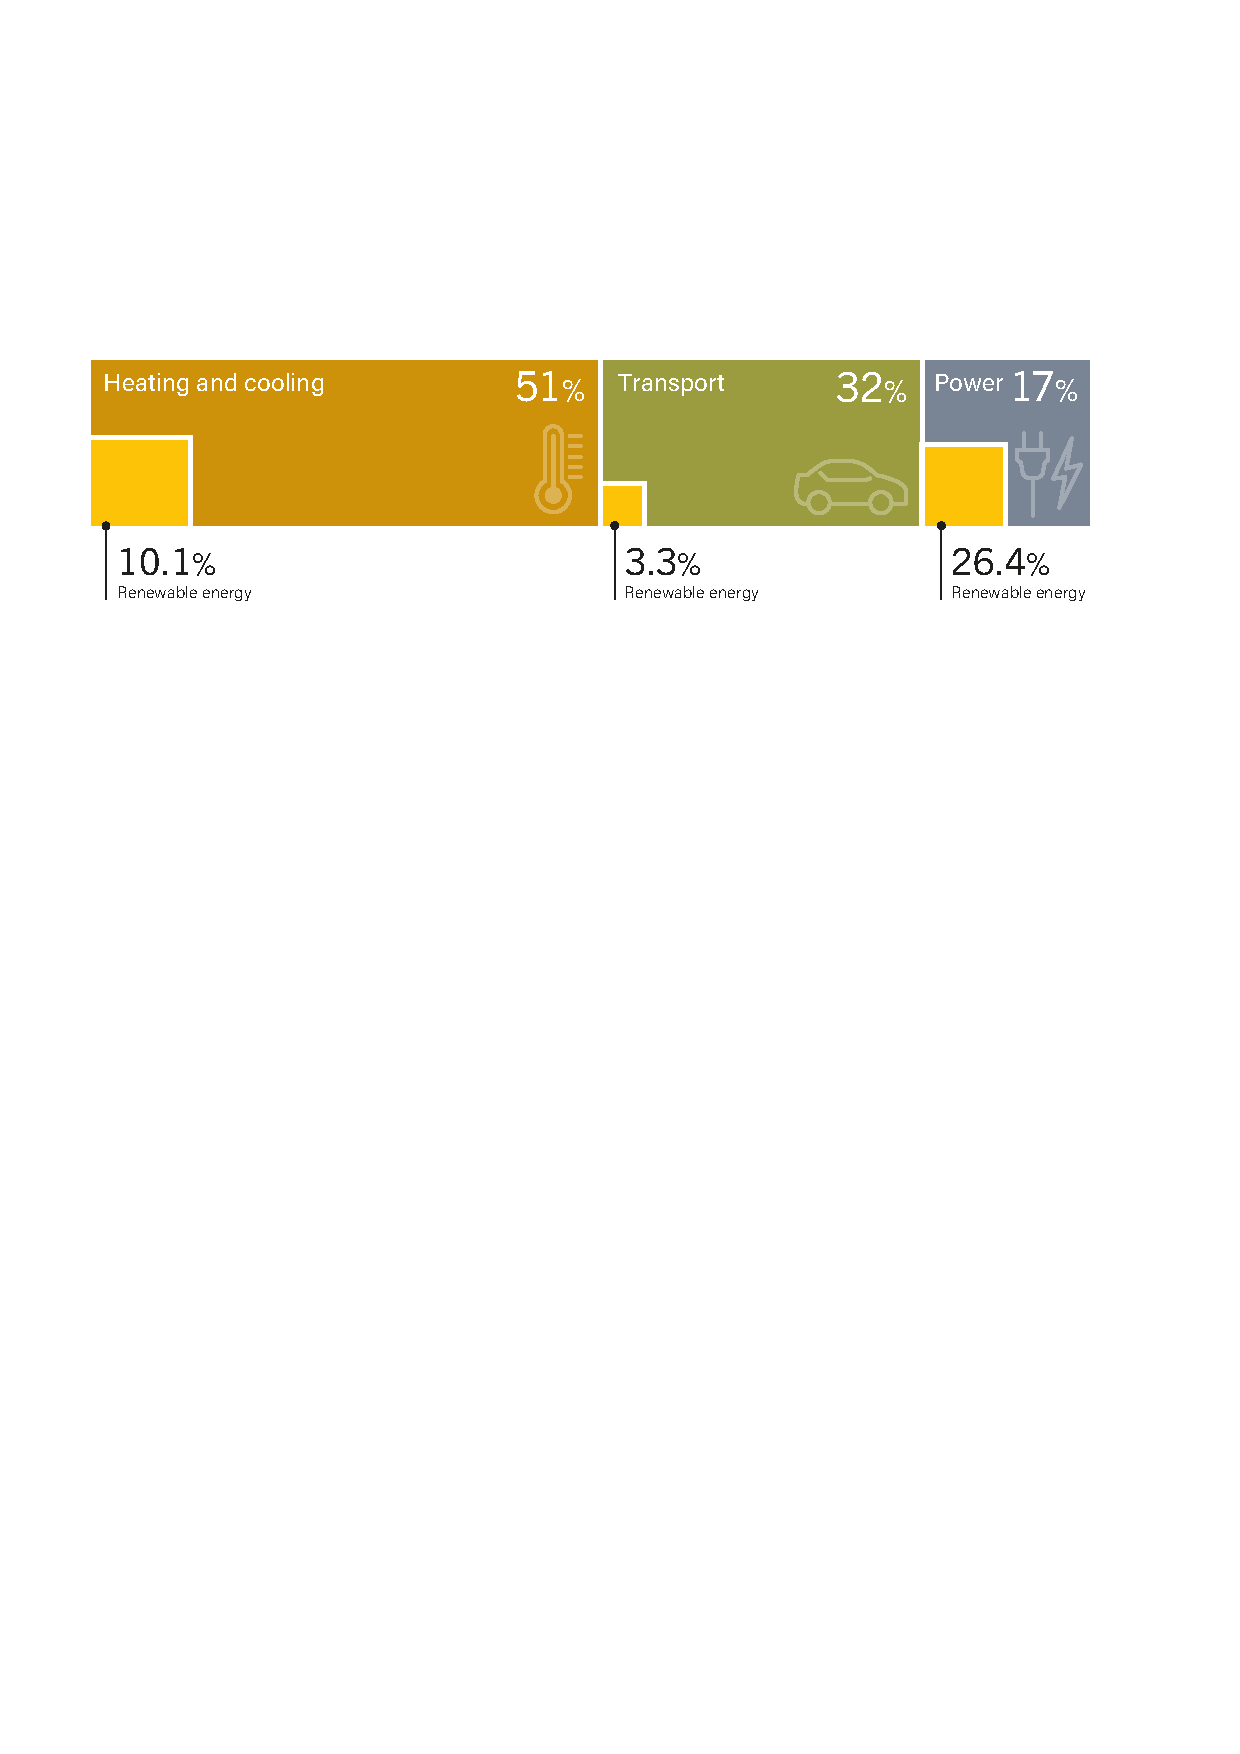
\includegraphics[width=\textwidth]{images/gsr_2020_RE_share.pdf} 
\caption[Renewable Share of Total Final Energy Consumption, by Final Energy Use, 2017]{Renewable Share of Total Final Energy Consumption, by Final Energy Use, 2017. Source: \citet{ren21_renewables_2020} (Based on IEA data)}
\label{fig:ren21_RE_use} 
\end{figure}
In this context, global energy reports highlight the current Covid-19 pandemic as a crucial opportunity to push towards more ambitious RE strategies \cite{iea_world_2020,irena_global_2020,fs-unep_global_2020}. 
The disruption to the energy sector caused by the pandemic exceed any event in history, and the consequences will last for years \cite{iea_world_2020}. 
As governments all around the world are developing huge recovery packages to support their societies and economies, aligning these packages with the medium and long-term goals of the Paris Agreement may lead to a "shift to sustainable, decarbonised economies and resilient inclusive societies" \cite{irena_global_2020}. 
The potential RE generation in urban environments is hereby of high interest, as cities are responsible for a large share of current global greenhouse gas emissions and are expected to host two thirds of the world population by 2050 \cite{irena_rise_2020}. 

Developing effective national and regional strategies to integrate RE into future energy systems requires knowledge of the potential energy generation from the available renewable resources. 
This includes information on \textit{which} technologies may provide a significant amount of energy, \textit{where} RE resources may be exploited and \textit{when} they are available. 
These aspects may be assessed through spatio-temporal modelling, which characterises both the spatial (\textit{"where"}) and temporal (\textit{"when"}) patterns of the energy generation from given RE resource.
The spatio-temporal modelling of RE potentials is however dependent on the availability of sufficient and high-quality data on the natural resources and the environment.
Rapid improvements in the quantity and quality of data collected at national and global levels, for example through satellite imagery, weather stations and land surveys, as well as in computational methods for data handling and analysis allows to assess these potentials in unprecedented ways.

% Paragraph: Switzerland
% Currently, there is no methodology that estimates the large-scale RPV potential at a high spatio-temporal resolution and also addresses the systematic propagation of uncertainties arising from the modelling process.
% This paper contributes to fill this gap by adapting state of the art methods for the assessment of RPV potential in order to quantify and combine different sources of uncertainty. 
% We further use Machine Learning to incorporate information that is only available in parts of the study region of Switzerland.
Motivated by the need for cross-sectoral RE policies, the push for RE incentives as part of  Covid-19-related recovery strategies and the opportunities presented through an increasing amount of energy-related data, this thesis aims to estimate a \textit{hybrid renewable energy potential} (HyREP) for the built environment at national scale. 
\nomenclature[A]{HyREP}{Hybrid Renewable Energy Potential}
The HyREP describes the spatial and temporal patterns of several renewable energy resources for electricity \textit{and} heat generation, which may be combined with other (non)-renewable energy sources to assess potential complementarities between energy sources and their potential for satisfying the energy demand of cities. 

% something about a database, focus on methodological aspects to have a spatially comparable potential, as well as establishing database
This thesis focuses on RE potential within the built environment, since the built environment gives rise to a large amount of the national electricity and heat demand. Directly satisfying this demand where it occurs reduces the need for heat and power transmission over large distances, which reduces losses and can help to reduce supply peaks due to the intermittency of RE resources. 
The focus of the work lies in the spatio-temporal estimation of the technical potential of RE sources at large scale, whereby the technical potential is defined as the maximum energy (heat or electricity) which can be provided using a specific RE technology. 
These resource potentials include physical, geographical and technical limitations and yield results at the scale of individual building or property units, at hourly or monthly temporal resolution for a large geographic area, such as the country of Switzerland. 

We assess the potential energy generation from two renewable resources which have been growing rapidly in Switzerland, namely rooftop solar photovoltaics (RPV) and ground-source heat pumps (GSHPs), which extract shallow geothermal heat at depths of < 400 m. 
The resource assessments form publicly available databases of RE potential, which can be used to study hybrid systems from neighbourhood to country scale based on data that is homogeneous across the country. 
By combining state-of-the-art analytical models of RE technologies with large-scale data processing techniques and advanced statistical methods, including Machine Learning (ML), the HyREP datasets presented in this thesis contain a high level of detail on the natural resources, the built environment and the modelled technologies.
\nomenclature[A]{ML}{Machine Learning}
To demonstrate how the renewable energy databases can be used for the study of hybrid energy systems (HES), this thesis concludes with an analysis of the potential self-coverage and self-sufficiency of urban neighbourhoods across the country through the large-scale deployment of RPV and GSHPs, setting these results in context with the Swiss Energy Strategy for 2050.
\nomenclature[A]{HES}{Hybrid Energy System}

% More specifically, the potential energy generation from two renewable resources is assessed, namely solar and geothermal energy. 
% The potential includes electricity and heat generation from rooftop-mounted solar photovoltaics (PV) and solar thermal collectors (STC), respectively, and heat generation from shallow (<400m) geothermal energy using borehole heat exchangers (BHE). 

% While to date individual aspects have been studied at national scale, no large-scale approach exists to model hybrid potential at high temporal and high spatial resolution to quantify the geographic distribution of storage requirements and maximum energy mismatch. Assessing for the first time the spatio-temporal distribution of hybrid energy potential on national scale can hence give a comprehensive view on the opportunities and risks of hybrid systems and on the regional and national energy balance. 

% Focusing on the Swiss energy landscape, this research aims to quantify the potential for distributed hybrid energy generation using state-of-the-art data-driven methods.

% END WITH SWITZERLAND

\section{A hybrid renewable energy potential for Switzerland}
\label{intro_REN}


Estimation of a hybrid renewable energy potential for Switzerland requires answering the following questions: 
\begin{itemize}
\item Which renewable energy resources are available in Switzerland?
\item How can the potential of these resources be spatially and temporally estimated?
\item What defines a hybrid renewable energy potential?
\end{itemize}

\subsection{Renewable energy in Switzerland}

Two types of renewable energies (RE) will be investigated in this study: solar energy and geothermal energy. These energies are amongst the fastest-growing RE in Switzerland in the last 10 years [1], with growth rates shown in Figure 1. Throughout this study, rooftop-mounted solar installations will be considered for electricity generation from photovoltaic (PV) panels, as well as for heat production for domestic heating and hot water applications from thermal collectors. Geothermal heat generation potential will be calculated for shallow depth (up to 400m) in accordance with current standards for domestic applications. Note that geothermal electricity generation is not considered as this technology is not applied in the domestic sector [2]. 

\begin{figure}[tb] 
\centering 
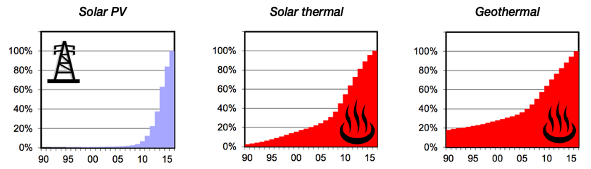
\includegraphics[width=\textwidth]{REN_CH} 
\caption[Growth rates of solar PV, solar thermal and geothermal technology application in Switzerland in the past 25 years.]{Growth rates of solar PV, solar thermal and geothermal technology application in Switzerland in the past 25 years. The data is given in \% of production for 2016 [1].}
\label{fig:ren_ch} 
\end{figure}

\subsubsection{Solar energy from photovoltaics and thermal collectors.}
As solar energy is abundantly available and easy to harvest, solar PV and solar thermal technologies have attracted worldwide interest. Most studies of solar potentials focus on PV potentials, for example in Switzerland [3]–[5], USA [6], Spain [7], [8], Germany [9], [10]. Solar thermal potentials on the large scale are rarely quantified; this may be partly due to a lower interest in solar thermal collectors for residential applications [1] and partly due to the high interdependency between collector efficiency and heat demand [11]. Large-scale potential studies have been carried out for thermal power plants in India [12], and for residential buildings in Switzerland [11]. Potentials are typically computed as monthly or yearly values; there is however no current study estimating the large-scale potential at an hourly timescale, which is necessary to quantify a potential for hybrid energy systems and requirements for energy storage. 

\subsubsection{Shallow geothermal energy from borehole heat exchangers}


\subsection{Spatio-temporal estimation of renewable energy potentials}

%% SOURCE: Research plan
For the computation of large-scale solar energy potentials, related studies widely apply a hierarchical approach [3], [4], [7], [13], illustrated in Figure 2. The first step is the calculation of a physical or theoretical potential, which represents the amount of energy that natural resources in the region of interest can provide (per unit area). In the second step, the geographic or urban potential is calculated, which accounts for the impact of the built environment on the natural resources. It measures the amount of energy that can be collected by the panels or collectors. The third step gives the technical potential and accounts for losses during conversion of the natural resources to domestic heat and electricity. It gives the maximum feasible amount of energy that can be harvested using a given technology. After obtaining the maximum feasible energy output, one may consider additional environmental, economic or social considerations to refine the estimated size of the system. A fourth step may thus be an economic potential focused on sizing the systems under given constraints. Economic considerations such as technology cost are not taken into account in the reviewed large-scale studies. Instead, they have been assessed in separate studies, in smaller-scale case studies as well as in hybrid potential assessments. An analysis of market potential is beyond the scope of this work. 
 
% Figure 2: Hierarchical approach for estimating rooftop PV and solar thermal potentials. [14]

\subsection{Definition of hybrid renewable energy potential}

\section{Research goals}
\label{intro_goals}
% SOURCE: Research plan
The main driver behind this study is the question whether it is possible to cover urban energy demand in Switzerland using a combination of renewable energies, and which level of energy autonomy could be reached in the built environment from this hybrid renewable energy potential. Special interest lies hereby on the spatial and temporal variability of the supply in order to match the seasonal and intra-day variations of the energy demand. With the focus on two types of resources, solar and geothermal energy, the following research questions arise:

\begin{itemize}
\item How can the potential for renewable energy resources in the built environment be estimated on national scale for Switzerland, and what are the related uncertainties?
\item What impact does the combination of multiple renewable resources to hybrid systems have on distributed energy supply?
\item How can data-driven methods and Machine Learning be applied to improve current ways of estimating potential and to facilitate their scalability to national scale?
\end{itemize}

The above questions have been partly addressed in case studies on building and district scale, or as large-scale studies of individual aspects, but no unified approach exists to assess hybrid energy potential for the built environment at high spatial and temporal resolution. Large-scale potential assessment has been performed in most cases in monthly resolution only, or without considering any spatial distribution of potentials. Many case studies have been conducted, but most models are computationally intensive and infeasible for application the large scale. Furthermore, a comprehensive analysis of uncertainties related to estimation and modelling is rarely provided. Machine Learning has been used in some studies, but there is still a huge potential that can be exploited to understand patterns in the available resources, approximate missing data and model system behaviour in a more computationally efficient way.

This study aims to combine methodologies of large-scale potential assessment and small-scale system modelling to quantify hybrid energy potential in the built environment for Switzerland. Data-driven methods and Machine Learning will be used to overcome gaps caused by lack of data and computational efficiency. The proposed assessment will make use of a large variety of environmental data and will present a unified approach that allows to compare the potential of some of the most promising renewable resources in the built environment. These resources will be combined with the energy demand to derive a hybrid potential which complements the demand patterns. The research hypothesis is hereby that hybrid systems in the built environment bring advantages over single-technology systems, and that a significant fraction of the energy demand can be covered by hybrid renewable potential if the energy mix is chosen appropriately.

The study is divided in three phases. The first phase focuses on electricity. It is divided into the computation of hourly solar energy potentials (WP1) and the assessment of hybrid electricity potential based on solar PV and wind energy (WP2). The second phase focuses on heat energy. In this phase, geothermal energy potentials will be evaluated (WP3) and combined with solar thermal potentials to a hybrid heat potential (WP4). A case study for a selected district will be conducted to assess multi-energy potentials and their effect on covering the urban energy demand. Finally, visualization methods for multi-dimensional data will be explored. 

% SOURCE: Research plan 
% The first phase of the study focuses primarily on electricity, i.e. the estimation of solar PV potential and its combination with electricity generation from wind and electricity demand (external inputs). During the second phase, heat systems with geothermal and solar thermal heat generation will be investigated. For the computation of potentials, data-driven modelling using Machine Learning algorithms is combined with parallelisation of analytical models to cope with the high spatial and temporal resolution of the relevant datasets. Geographic information systems (GIS) are further used to handle geographically referenced datasets. Efforts are made to quantify the uncertainty related to several modelling steps throughout the study and to identify the sources of uncertainties, for example caused by modelling or by data noise.

\section{Structure of the thesis}
To address the above research goals, the thesis is structured as follows:

\textbf{Part~\ref{methods}} provides a summary of state-of-the-art analytical and statistical methods used in the thesis and large-scale datasets used in the national REN potential studies. \textbf{Chapter~\ref{methods_physical}} introduces analytical methods for modelling physical processes and technological aspects of RPV and GSHP systems. \textbf{Chapter~\ref{methods_ML}} covers Machine Learning methods used in this work and stastical approaches for uncertainty estimation.  \textbf{Chapter~\ref{data}} provides an overview over the available meteorological, environmental and building-related datasets for Switzerland.

\textbf{Part~\ref{potential} }addresses the estimation of renewable energy potentials. \textbf{Chapter~\ref{solar} } details the developed model for estimating rooftop solar photovoltaic potential at national scale, as well as a  comparison of the resulting potential database with existing estimations for Switzerland. \textbf{Chapter~\ref{geothermal}} provides the estimation of technical potential for shallow geothermal energy, using analytical models at regional scale and Machine Learning for the estimation at national scale. The chapter further shows an approach to expand the model to include thermal regeneration of the geothermal resources through cooling re-injection to the ground with regional-scale application.

\textbf{Part~\ref{hybrid}} demonstrates the application of the potential databases developed in Part~\ref{potential} for modelling hybrid renewable energy systems. \textbf{Chapter~\ref{hybrid_chapter}} outlines a mapping approach for the energy demand of heat and electricity from readily available data, which is a necessary complementary input to perform hybrid system studies. [TO BE CONTINUED].

\textbf{Chapter~\ref{conclusion}} concludes with the main findings of the thesis and a future outlook.




\cleardoublepage

\part{State-of-the-art methods and data}
\label{methods}
% \chapter{Methods and data}

\chapter{Modelling renewable energy technologies}
\label{methods_physical}

\vspace{-15pt} % -15pts for two-line heading, -45pts for single-line heading
\begin{tcolorbox}[enhanced,width=\textwidth,size=fbox,
        sharp corners,colframe=black!5!white,drop fuzzy shadow southeast,
        boxrule=3mm, parbox=false] 
        
This chapter borrows from the articles \citep{walch_big_2020,walch_quantifying_2021}:

\qquad \bibentry{walch_big_2020}

\qquad \bibentry{walch_quantifying_2021}
\end{tcolorbox}

Spatio-temporal modelling of renewable energy potentials integrates physical models of the renewable resources and technologies with geospatial operations using Geographic Information Systems (GIS).
The present chapter introduces state-of-the-art modelling approaches for two types of renewables addressed in this thesis, namely rooftop solar energy (Section \ref{method_solar}) and shallow geothermal energy (Section \ref{geo_method}). 
\nomenclature[A]{GIS}{Geographic Information Systems}
Relevant physical, geographical and technical constraints for both energy resources are outlined and popular modelling approaches are summarized, such as to justify the methods used in the large-scale estimation of rooftop solar potential (Chapter \ref{solar}) and shallow geothermal potential (Chapter \ref{geothermal}).

\section{Rooftop solar energy}
\label{method_solar}
\label{method_solar_hierarchy}
% and solar thermal 

Rooftop solar energy is defined here as the electrical or thermal energy harvested from installations on building rooftops, using solar photovoltaic (PV) panels or solar thermal collectors (STC), respectively. 
While we focus on the estimation of solar photovoltaic (PV) potential, which is currently the most frequently deployed solar technology on rooftops \cite{kaufmann_schweizerische_2017}, most parts of the methodology (except the techological model of the solar PV panels) are transferable to STC. 
\nomenclature[A]{STC}{Solar thermal collector}
\nomenclature[A]{RPV}{Rooftop photovoltaics}
This section reviews state-of-the-art approaches to model the hourly energy yield of rooftop-mounted solar PV systems in the context of large-scale potential studies, and justifies the choice of the empirical models (Section~\ref{phys_models}), geospatial techniques (Section~\ref{GIS_methods}) and the modelling approach for PV panels on flat roofs (Section~\ref{app_flat}) used in the large-scale rooftop PV potential estimation presented in Chapter~\ref{solar}. We hereby do not claim to provide a complete review of existing modelling approaches, but rather give an overview of the relevant modelling steps and outline popular computational methods for each step.

\begin{figure}[tb]
	\centering
	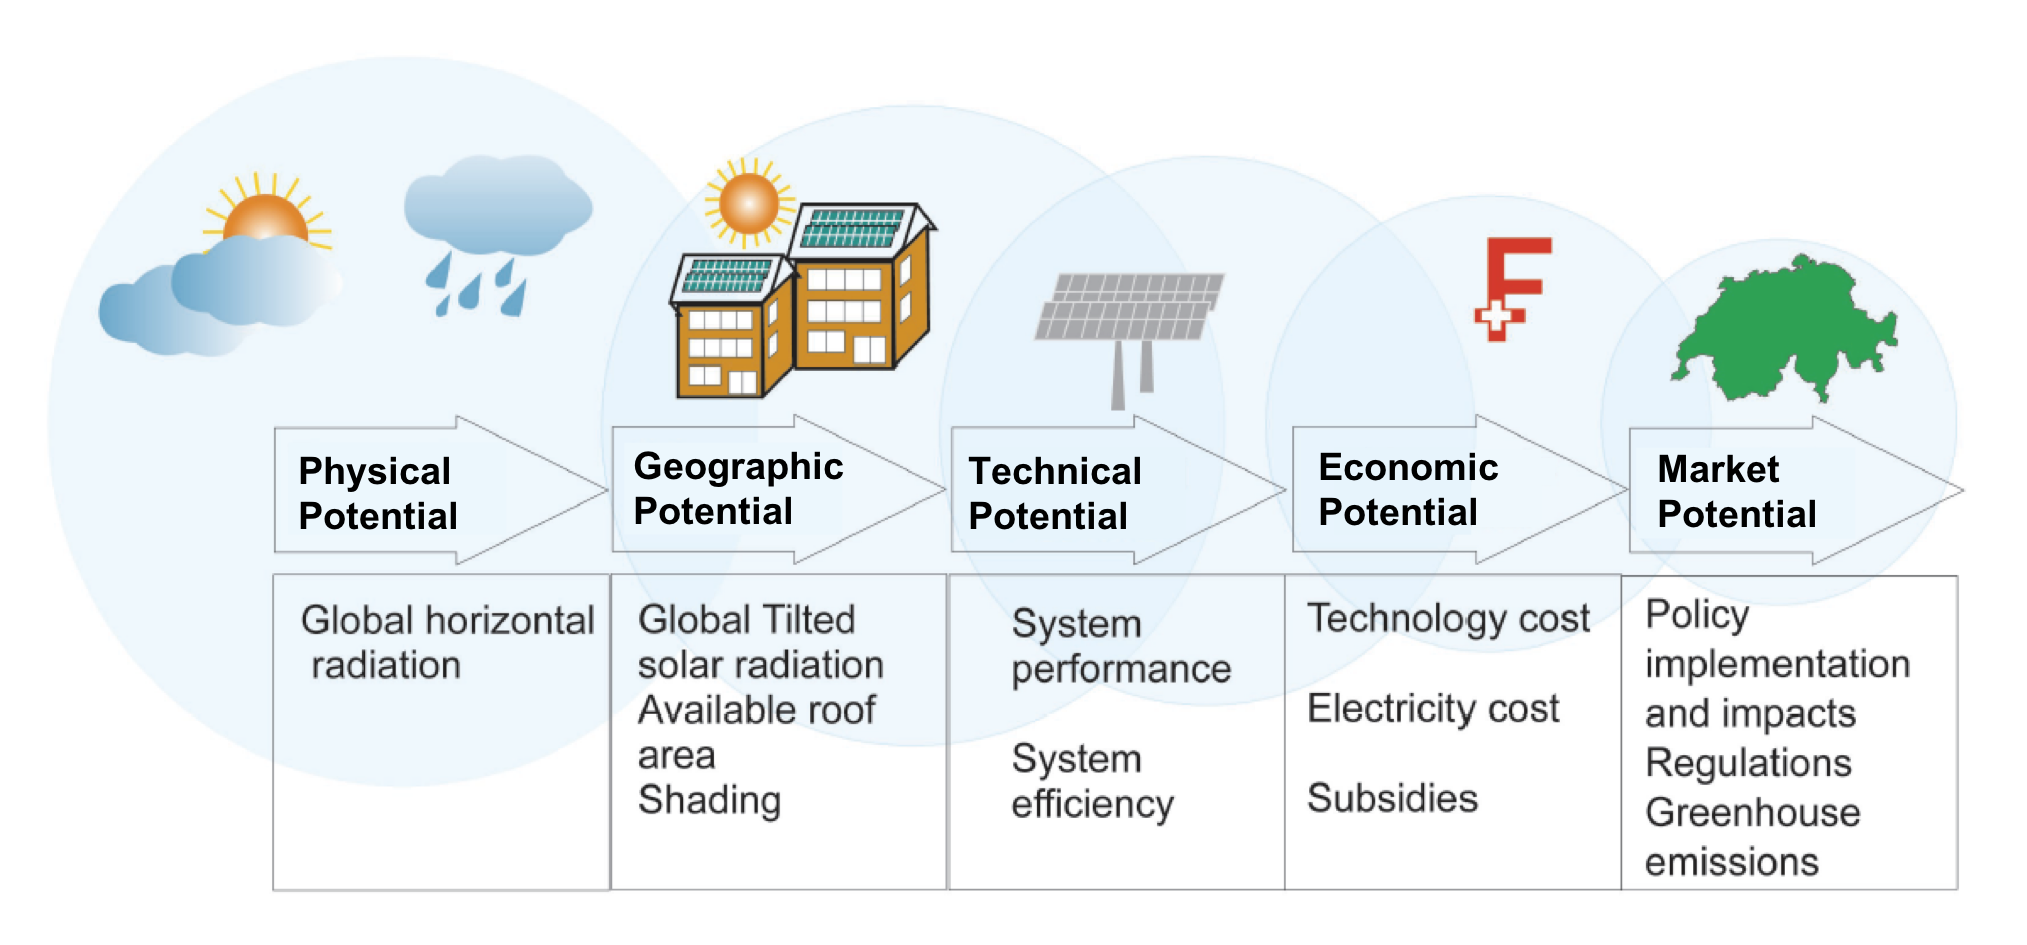
\includegraphics[width=\linewidth]{images/Figs/hierarchy.png}  
	\caption{Hierarchical approach for estimating rooftop PV potential. Source: \citet{assouline_estimation_2017}}
	\label{fig:solar_hierarchy}
\end{figure}

% SOURCE: CISBAT comparison paper
To compute the technical rooftop PV potential,  a hierarchical approach, shown in Fig.~\ref{fig:solar_hierarchy}, has been widely accepted in the literature \cite{assouline_quantifying_2017,ramirez_camargo_spatio-temporal_2015,izquierdo_method_2008,wiginton_quantifying_2010}. It includes (i) \textit{physical potential}, that is, the amount of solar energy reaching the earth’s surface, (ii) \textit{geographic potential}, that is, the amount of solar radiation received by the tilted PV panels, which is affected by the geometry of the panel (slope and aspect), the shading from surrounding buildings and trees and the suitable area for the panel installation, and (iii) \textit{technical potential}, that is, the maximum electricity output considering the technical characteristics of the PV technology (e.g. efficiency and system performance).

After obtaining the maximum feasible electricity output, one may consider additional environmental, economic or social considerations to refine the estimated size of the system. A fourth step may thus be an \textit{economic potential} focused on sizing the systems under given constraints. Economic considerations such as technology cost are not taken into account in most large-scale studies. Instead, these are typically assessed in separate studies that use the technical PV potential as input, in smaller-scale case studies as well as in hybrid potential assessments. An analysis of \textit{market potential} is beyond the scope of this work. 

\textbf{Physical potential.} The incoming solar radiation (also referred to as irradiance, in W/m$^2$), consists of three compotents: (i) a direct or beam component ($G_B$), which describes the direct incoming solar radiation on a horizontal plane, (ii) a diffuse component ($G_D$), which is diffracted for example through the atmosphere and through cloud coverage, and (iii) a surface reflected component $G_R$, which is driven by the ground surface reflectance, also known as albedo ($\rho$), but which can be omitted for horizontal planes \cite{assouline_estimation_2017}. Omitting $G_R$, the global horizontal solar radiation $G_h$ is given by \cite{assouline_estimation_2017}:
\begin{equation}
\label{eq:Gh_method}
G_{h} = G_{B} + G_{D}
\end{equation}
While most large-scale studies of RPV potential use satellite data or station measurements to obtain $G_h, G_B, G_D$ (e.g. \cite{bodis_high-resolution_2019,buffat_scalable_2018,ramirez_camargo_spatio-temporal_2015,calcabrini_simplified_2019}), empirical models exist to derive these from related variables such as the sunshine duration and the extra-terrestrial solar radiation \cite{assouline_estimation_2017}. 
In other cases, (geo)-statistical methods have been developed to estimate solar radiation. 
These include averaging the nearest neighbours \cite{klauser_solarpotentialanalyse_2016}, geostatistical methods such as kriging \cite{alsamamra_comparative_2009,rehman_spatial_2000} as well as machine learning approaches such as Support Vector Machines \cite{assouline_quantifying_2017}, Random Forests \cite{assouline_large-scale_2018} and neural networks \cite{hocaoglu_hourly_2008,notton_neural_2013,sahin_application_2013}. As averaging tends to oversimplify the modelling, and kriging is computationally intensive and requires modelling of anisotropic spatial correlations and stationarity of the process, the data-driven machine learning algorithms have recently gained much attention due to their performance and speed \cite{kanevski_machine_2009}. 
Most models do not estimate the uncertainty related to modelling horizontal irradiance, which is an important aspect if the results are processed further.
A further review of different modelling techniques for horizontal solar radiation is provided in \cite{zhang_review_2018}.

\textbf{Geographic potential.} The solar power received by RPV panels is driven by two factors: (i) the incoming solar radiation on the tilted panels, and (ii) the available area for installing PV, sometimes also quantified as the number of panels that can be installed on a rooftop. As the global horizontal radiation, the tilted radiation ($G_t$) is composed of a direct ($G_{Bt}$), a diffuse ($G_{Dt}$) and a reflected ($G_{Rt}$) component, such that \cite{assouline_estimation_2017}:
\begin{equation}
\label{eq:POA}
G_{t} = G_{Bt} + G_{Dt} + G_{Rt}
\end{equation}

The three components in Eq.~\ref{eq:POA} describe the plane-of-array (POA) radiation, obtained from empirical models (Section~\ref{phys_models}), which represents the radiation received by a fully unshaded PV panel in an open space. 
In urban environments, however, direct shading and a reduced sky visibility from surrounding buildings or other built-up objects, referred to as the sky view factor (SVF), can significantly impact the electricity yield of a PV panel. 
Hence, many studies of rooftop PV potential use geospatial techniques based on 2D or 3D models of the urban environment, detailed in Section~\ref{GIS_methods}, to quantify shading effects and the SVF (e.g.~\cite{desthieux_solar_2018,calcabrini_simplified_2019,wegertseder_combining_2016,jakubiec_method_2013}).
As these are included across the literature in the form of different factors, partially due to different spatial and temporal resolutions of RPV studies, we do not provide a generalised formulation to include these factors in Eq.~\ref{eq:POA}. However, in Chapter~\ref{solar_comparison} we will attempt to formulate such a generalisation for studies carried out in Switzerland.

The available area for installing PV or STC ($A_{PV}$) is potentially the factor that varies most between different studies of RPV potential, as it is strongly dependent on the scale of the study and on the available rooftop data. 
Rooftop available area is either quantified as constant factors (e.g. \cite{iea_potential_2002,wegertseder_combining_2016,portmann_sonnendach.ch:_2016}) or derived from building data (\cite{ramirez_camargo_spatio-temporal_2015,assouline_quantifying_2017,hong_development_2017}) and aerial imagery \cite{mainzer_assessment_2017} using geospatial techniques or image processing. 
As the required geospatial input data may not be available across entire study areas and the computational time for these methods may be prohibitively high, sampling techniques \cite{izquierdo_method_2008}, the use of building prototypes \cite{wegertseder_combining_2016} and extrapolation techniques using ML \cite{assouline_quantifying_2017,assouline_large-scale_2018} based on geospatial methods are frequently used in large-scale studies. 
A review of statistical and geospatial techniques for quantifying the available roof area is provided in Section~\ref{GIS_methods}, differentiating between the quantification of the total roof area, the useful roof area and the roof suitability for PV installations.

\textbf{Technical potential.} The conversion of global radiation to PV potentials is driven by three factors: the efficiency of the PV panel ($\eta_{PV}$), the inverter efficiency ($\eta_\mathit{inv}$) and other losses ($\eta_\mathit{losses}$), which are multiplied with the tilted radiation ($G_t$) and the available area for PV installation ($A_{PV}$):
\begin{equation}
    P_{PV} = G_t \times A_{PV} \times \eta_{PV} \times \eta_\mathit{inv} \times \eta_\mathit{losses}
\end{equation}
While several studies use constant values for panel and inverter efficiencies \cite{assouline_quantifying_2017,wegertseder_combining_2016,romero_rodriguez_assessment_2017,ordonez_analysis_2010,hong_development_2017}, many high-resolution PV potential studies use analytical or empirical models to quantify the efficiencies as a function of radiation, temperature, wind speed and technical characteristics of PV systems. The level of detail of these models ranges from the analytical modelling of invidual cells and their arrangement in a PV panel \cite{buffat_scalable_2018} to entirely coefficient-based empirical models \cite{mainzer_assessment_2017} (see Section~\ref{phys_models}). Other losses, however, are accounted for as constant loss factors in most studies. These may account for panel soiling, degradation, network and wiring losses, partial shading of panels and other factors.

An overview of these parameters used to estimate the physical, geographic and technical PV potential and a summary of popular methods to compute these parameters is provided in Table~\ref{tab:solar_methods_compare}.

\begin{table}[htbp]
\centering
\footnotesize
\caption{Parameters for estimating the physical, geographic and technical potential and a (non-exhaustive) review of methods to compute these parameters.}
\label{tab:solar_methods_compare}
\resizebox{\textwidth}{!}{%
\begin{tabular}{llllll}
\hline
\textbf{Type} & \textbf{Parameters} & \textbf{Unit} & \textbf{Description} & \textbf{Methods (selected)} & \textbf{References} \\ \hline
\multirow{4}{*}{\begin{tabular}[c]{@{}l@{}}\textit{Physical}\\ \textit{potential}\end{tabular}} & \multirow{4}{*}{$G_h, G_B, G_D$} & \multirow{4}{*}{W/m$^2$} & \multirow{4}{*}{\begin{tabular}[c]{@{}l@{}}Global, direct, diffuse\\ horizontal solar radiation\end{tabular}} & Satellite / measured data & \cite{bodis_high-resolution_2019,buffat_scalable_2018,ramirez_camargo_spatio-temporal_2015,calcabrini_simplified_2019} \\
 &  &  &  & Empirical models & \cite{assouline_estimation_2017} \\
 &  &  &  & Kriging &  \cite{alsamamra_comparative_2009,rehman_spatial_2000}  \\
 &  &  &  & Machine Learning & \cite{assouline_quantifying_2017,assouline_large-scale_2018,hocaoglu_hourly_2008,notton_neural_2013,sahin_application_2013} \\ \hline
\multirow{11}{*}{\begin{tabular}[c]{@{}l@{}}\textit{Geographic}\\ \textit{potential}\end{tabular}} & $G_t$ & \multirow{4}{*}{W/m$^2$} & Tilted (POA) radiation & $G_t = G_{Bt} + G_{Dt} + G_{Rt}$ &  \\
 & $G_{Bt}, G_{Rt}$ &  & Direct, reflected component & Geometric projection & \cite{gulin_estimation_2013} \\
 & \multirow{2}{*}{$G_{Dt}$} &  & \multirow{2}{*}{Diffuse component} & Perez model & \cite{perez_modeling_1990, buffat_scalable_2018,jakubiec_method_2013,mainzer_assessment_2017,wegertseder_combining_2016} \\
 &  &  &  & Other (Hay, Liu-Jordan, Klein) & \cite{desthieux_solar_2018,izquierdo_method_2008,singh_estimation_2015, assouline_estimation_2017}  \\ \cline{2-6} 
 & \multirow{3}{*}{\begin{tabular}[c]{@{}l@{}}SVF / \\ Shading\end{tabular}} & \multirow{3}{*}{-} & \multirow{3}{*}{\begin{tabular}[c]{@{}l@{}}Sky view factor /\\ Shaded roof area\end{tabular}} & Fisheye images &  \cite{calcabrini_simplified_2019}\\
 &  &  &  & Digital surface model/LiDaR & \cite{jakubiec_method_2013,desthieux_solar_2018,hong_development_2017,strzalka_large_2012} \\
 &  &  &  & Roof fraction (constant) & \cite{mainzer_assessment_2017,wiginton_quantifying_2010, izquierdo_method_2008} \\ \cline{2-6} 
 & \multirow{4}{*}{APV} & \multirow{4}{*}{m$^2$} & \multirow{4}{*}{Available roof area} & Entire roof area & \cite{ramirez_camargo_spatio-temporal_2015,buffat_scalable_2018,hong_development_2017} \\
 &  &  &  & Roof fraction (constant) & \cite{iea_potential_2002,wegertseder_combining_2016,portmann_sonnendach.ch:_2016,wiginton_quantifying_2010}  \\
 &  &  &  & Derived from geospatial data & \cite{assouline_large-scale_2018,ordonez_analysis_2010, mainzer_assessment_2017} \\
 &  &  &  & Extrapolation to the large-scale & \cite{izquierdo_method_2008, wegertseder_combining_2016,assouline_quantifying_2017} \\ \hline
\multirow{3}{*}{\begin{tabular}[c]{@{}l@{}}\textit{Technical}\\ \textit{potential}\end{tabular}} & \multirow{2}{*}{$\eta_{PV}, \eta_{\mathit{inv}}$} & \multirow{2}{*}{-} & \multirow{2}{*}{\begin{tabular}[c]{@{}l@{}}PV panel, inverter \\ efficiency\end{tabular}} & Empirical model & \cite{jakubiec_method_2013,ramirez_camargo_spatio-temporal_2015,lukac_buildings_2014,buffat_scalable_2018,mainzer_assessment_2017,calcabrini_simplified_2019} \\
 &  &  &  & Constant value &  \cite{wegertseder_combining_2016,romero_rodriguez_assessment_2017,ordonez_analysis_2010,assouline_quantifying_2017,hong_development_2017,bodis_high-resolution_2019} \\
 & $\eta_{\mathit{losses}}$ & - & \begin{tabular}[c]{@{}l@{}}System losses (Soiling, wiring,\\ degradation etc.)\end{tabular} & Constant value & \cite{klauser_solarpotentialanalyse_2016,buffat_scalable_2018,mainzer_assessment_2017,lorenz_regional_2011,bodis_high-resolution_2019} \\ \hline
\end{tabular}
}
\end{table}

\begin{comment}
The panel efficiency is dependent on the selected technology and lies typically between 15-20\%. The performance ratio considers several external factors affecting the system’s performance, such as operating temperature, panel obstruction or converter losses. It can thus be calculated using an analytical formula [9], in most large-scale studies it is however approximated as 80\% [3], [5], [6]. Given the global irradiance on tilted surfaces Gt, the useful rooftop area AR, the power factor PF and the panel efficiency $\eta_{PV}$, the total PV power output per rooftop $P_{PV}$ (in $W$) can hence be calculated as:
\end{comment}

\subsection{Empirical models}
\label{phys_models}

Empirical models are widely used in the modelling of the electricity yield of RPV systems, as they allow to estimate relevant physical variables with little computational effort and from widely available data. 
In particular, empirical models are used in the literature (i) to quantify the plane-of-array (POA) radiation, namely the tilted radiation components ($G_{Bt}, G_{Dt}, G_{Rt}$) incident to the inclined PV panels, and (ii) for modelling solar PV technology, more specifically the efficiency of the PV panel and the inverter, which converts the direct current (DC) PV output to "grid-level" alternating current (AC). 

%% SOURCE: Research plan
%To compute the potential energy output, firstly the amount of solar power reaching a tilted panel/collector surface must be computed. This quantity is defined as global solar irradiance and given in W/m2. It consists of 3 components: a direct or beam component, a diffuse component and a reflected component (see Figure 3a). They are calculated from measurements of global horizontal (GHI), direct normal (DNI) and diffuse horizontal irradiance (DHI). Direct normal irradiance is converted to the tilted beam component via a geographic projection shown in Figure 3b. Diffuse tilted irradiance is more complex to determine due to its diffracted nature. Several models exist with different assumptions and hence varying complexity. Gueymard [15] compared several of these models and compared their approximation errors under different operating conditions. While no model clearly outperforms the other models, his analysis shows the Klucher method [16] amongst the best in most scenarios. The reflected component is given by another geometric conversion based on the ground’s surface reflectance. The mathematical formulae for the conversions are demonstrated for example by Gulin et al. [17].

% Figure 3: a) three solar irradiance components reach a solar panel: direct (beam), diffuse and reflected irradiance; b) geometry for calculating the angle of incidence of direct beam irradiance on a tilted plane;  , : surface tilt & azimuth, z : apparent sun zenith,  : angle of incidence [17]

\subsubsection{Plane-of-array radiation}
\label{app:irrad}

\begin{figure}[tb]
\centering
\begin{subfigure}[t]{.43\textwidth}
  \centering
  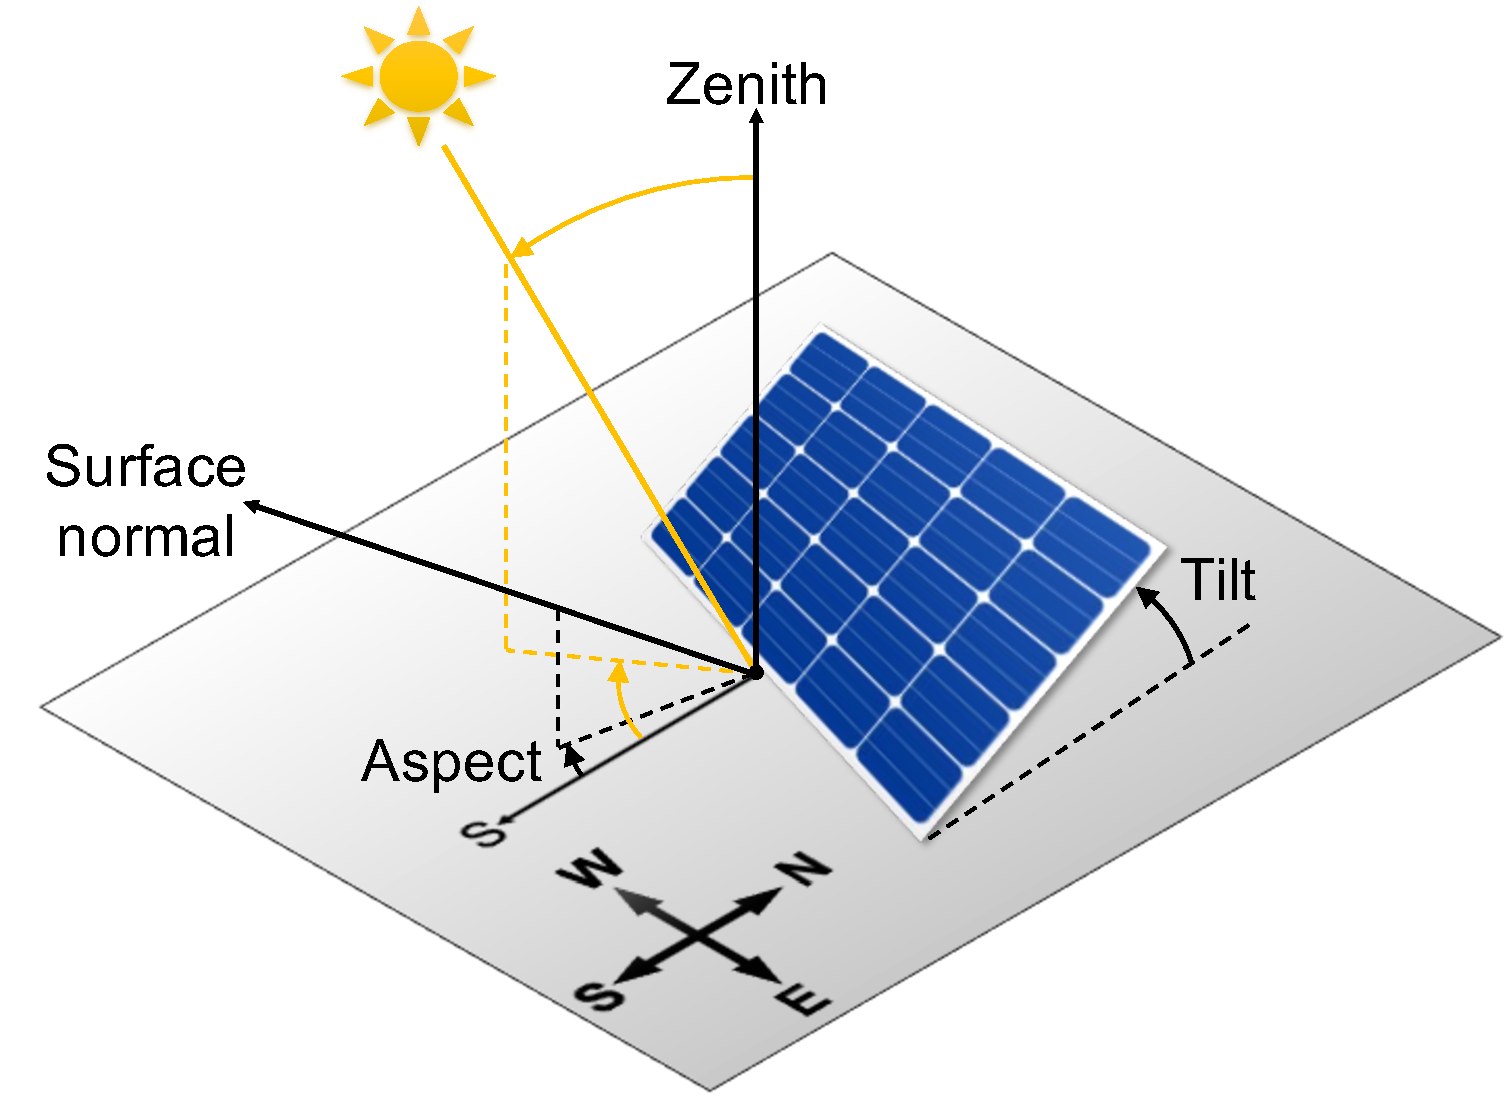
\includegraphics[width=\linewidth]{images/Figs/poa.pdf}  
    \subcaption{}
  \label{figa:solar_geom}
\end{subfigure}
\begin{subfigure}[t]{.53\textwidth}
  \centering
  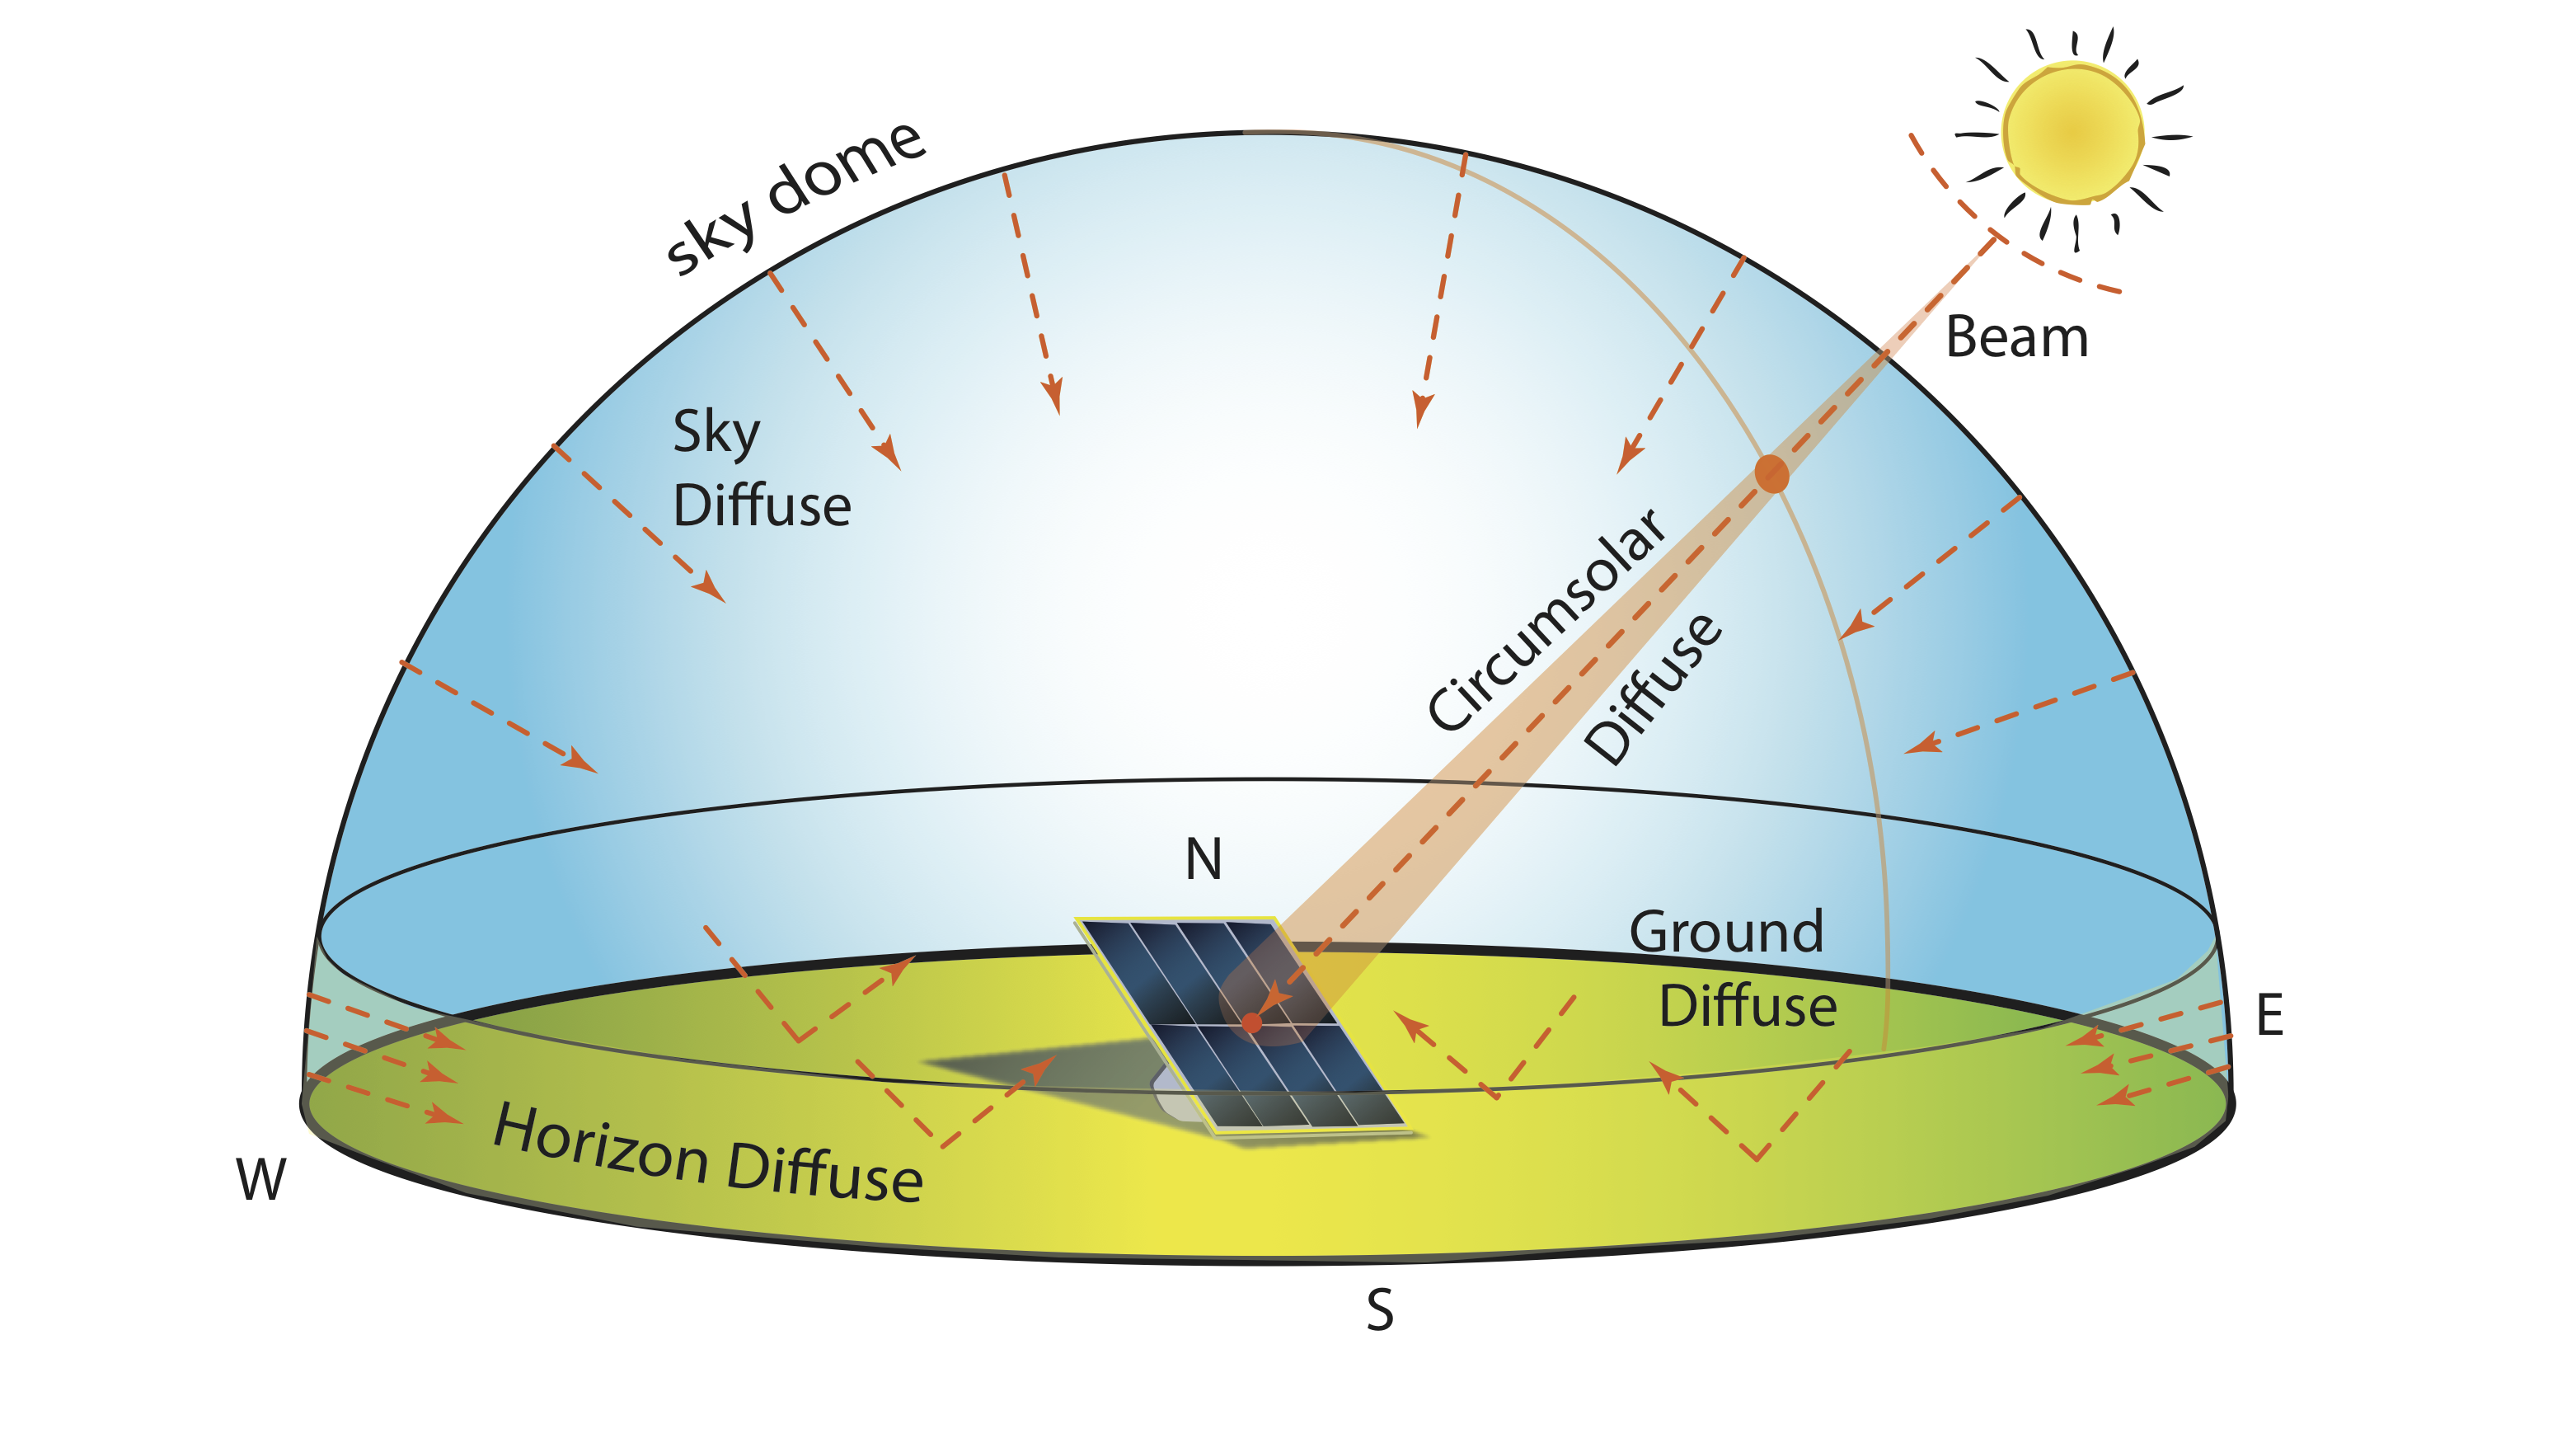
\includegraphics[width=\linewidth]{images/Figs/diffuse_components.png}  
    \subcaption{}
  \label{figb:solar_geom}
\end{subfigure}
\caption{Geometrical models for calculating (a) the angle of incidence of direct beam radiation on a tilted plane, and (b) the isotropic, circumsolar and horizon diffuse components (Source: \citet{brownson_44_nodate}).}
\label{fig:solar_geom}
\end{figure}

To compute the direct, diffuse and reflected tilted irradiance components $G_{Bt}$, $G_{Dt}$ and $G_{Rt}$, empirical and geometrical models are widely accepted in the literature. 
The direct component is obtained from a geometrical projection of the horizontal $G_B$ on the angle of incidence of the sun rays on the tilted panel ($\theta$) (see Fig.~\ref{figa:solar_geom}). Mathematicaly, this projection is defined as \cite{gulin_estimation_2013}:

\begin{equation}
\label{eq:direct}
    G_{Bt} = G_{B} * \max \left( 0, \frac{\cos(\theta)}{\cos(\theta_Z)} \right)
\end{equation}

where
\begin{equation}
\label{eq:dir_angle}
\cos(\theta) = \sin(\beta) \sin(\theta_Z) \cos(\gamma_S - \gamma) + \cos(\beta) \cos(\theta_Z) 
\end{equation}

The angles $\theta_Z$ and $\gamma_S$ describe the sun zenith and azimuth angles, respectively, while roof tilt and aspect are given by $\beta$ and $\gamma$.

Diffuse tilted irradiance is more complex to determine due to its diffracted nature. Several models exist with different assumptions and hence varying complexity. \citet{assouline_estimation_2017} review these different models and compares the temporal resolutions for which they are applicable.
Of the methods listed in \citet{assouline_estimation_2017} , the Perez model ~\cite{perez_modeling_1990} is the most frequently used model in the reviewed literature \cite{buffat_scalable_2018,jakubiec_method_2013,mainzer_assessment_2017,wegertseder_combining_2016}, and will also be used throughout this thesis.
The empirical formula for $G_{Dt}$ using the Perez model is given by~\cite{perez_modeling_1990}:

\begin{equation}
\label{eq:diffuse}
G_{Dt} = G_D * \left[ (1 - F_1) \left( \frac{1 + \cos \beta}{2} \right) 
       + F_1 \frac{ a }{ b }
       + F_2 \sin \beta \right]
\end{equation}

where $F_1$ and $F_2$ are empirically fitted functions for the circumsolar and horizon brightness, and $a$, $b$ are geometric angles. The derivation of these factors is described in \cite{loutzenhiser_empirical_2007}. The three addends in Eq.~\ref{eq:diffuse} represent an isotropic component, a circumsolar component originating from the sun disk (modelled as a point source) and a horizon component respectively, as shown in Fig.~\ref{figb:solar_geom}.

The reflected radiation ($G_{Rt}$) is again obtained from a widely used geometric projection based on the surface albedo $\rho$, which is defined as \cite{duffie_solar_2013}:

\begin{equation}
\label{eq:reflected}
G_{Rt} = G_h * \rho \left( \frac{1-\cos \beta}{2} \right)
\end{equation}

To ease the notation, Equations~\ref{eq:direct}-\ref{eq:reflected} can be referred to as:
\begin{equation}
\label{eq:tilted_irrad_simplified}
G_{Bt} = F_B G_B, \quad G_{Dt} = F_D G_D, \quad G_{Rt} = F_R G_h
\end{equation}



\subsubsection{PV module and inverter efficiency}
\label{app:efficiency}

In contrast to the modelling of the POA radiation, various empirical models exist to compute the electricity yield of PV systems. 
To compute the panel efficency ($\eta_{PV}$), the most detailed models simulate the maximum power point of the PV panel using single-diode current voltage equations \cite{strzalka_large_2012,buffat_scalable_2018}.
Most studies use a more generalised approach, which models $\eta_{PV}$ as a function of $G_t$, the PV cell temperature (derived from the ambient temperature) and the nominal performance rating of the PV panel \cite{jakubiec_method_2013,calcabrini_simplified_2019,singh_estimation_2015,ramirez_camargo_spatio-temporal_2015,mainzer_assessment_2017}. \citet{jakubiec_method_2013} compare PV efficiency models for widely used tools for two test buildings.

A general formulation of the DC power output of a PV panel ($P_{dc}$) is formulated in the \textit{PVWatts} model developed by the National Renewable Energy Laboratory (NREL) \cite{dobos_pvwatts_2014}, which is used in similar formulations for example in \cite{jakubiec_method_2013,ramirez_camargo_spatio-temporal_2015,singh_estimation_2015,calcabrini_simplified_2019}. 
In this work, we follow these studies, modelling the DC power output of a PV panel as:
\begin{equation}
\label{eq:Pdc}
    P_{dc} = \frac{G_{t}}{1000} P_{dc0} (1 + \gamma_\mathit{pdc}(T_\mathit{cell}-T_\mathit{ref}))
\end{equation}
where $G_t$ is the tilted radiation, $P_{dc0}$ is the DC rating of the panel,  $\gamma_\mathit{pdc}$ is its temperature coefficient, $T_\mathit{cell}$ is the cell temperature and $T_\mathit{ref}$ is the reference temperature.
%
We use average panel specifications of mid-range 60-cell mono-crystalline PV modules, the most frequently used technology in Switzerland \cite{buffat_scalable_2018}, from three market-leading manufacturers (JA Solar, Jinko Solar, Trinasolar). The values are reported in Table~\ref{tab:efficiency}.
%
From the DC power output and the area of a PV panel ($A_\mathit{panel}$), the module efficiency $\eta_{PV}$ is computed as:

\begin{equation}
\label{eq:eff}
    \eta_{PV} = \frac{P_{dc}}{G_{t} * A_\mathit{panel} }
\end{equation}
With the exception of \cite{calcabrini_simplified_2019}, the cell temperature is computed in the literature through a linear combination of the ambient temperature $T_\mathit{amb}$ and $G_t$, whereby $G_t$ is multiplied with a constant coefficient based on nominal operating conditions and corrected for the roof absorptivity and radiative heat losses \cite{jakubiec_method_2013}.
%
In this work, we use the \textit{PVSyst} model~\cite{faiman_assessing_2008} to derive $T_{cell}$ from $G_t$ and $T_\mathit{amb}$:

\begin{equation}
    T_\mathit{cell} = T_\mathit{amb} + G_t \frac{\alpha (1 - \eta_m)}{U}
\end{equation}
where $\alpha$ denoted the absorption coefficient, $\eta_m$ denotes the module efficiency and $U$ is the heat transfer component, for which we use default values for rooftop-mounted PV systems as suggested by Sandia National Laboratories \cite{holmgren_pvlib_2018} (Table~\ref{tab:efficiency}).

In contrast to Eq.~\ref{eq:Pdc}, which is based on physical principles, the inverter effiency ($\eta_\mathit{inv}$) is modelled using a fully empirical formula with three free parameters. Out of the various sets of coefficients in the literature \cite{mainzer_assessment_2017,lukac_buildings_2014}, we use the empirical loss formula from \textit{PVWatts}, also used in \cite{buffat_scalable_2018}, for consistency with Eq.~\ref{eq:Pdc}. It is defined as \cite{dobos_pvwatts_2014}:

\begin{equation}
\label{eq:inv}
    \eta_{inv} = \frac{\eta_{nom}}{\eta_{ref}} \left( -0.0162 * \zeta - \frac{0.0059}{\zeta} + 0.9858 \right)
\end{equation}

where $\zeta = P_{dc}/P_{dc0}$, $\eta_{nom}$ is the nominal inverter efficiency and $\eta_{ref}$ is the reference efficiency (see Table \ref{tab:efficiency} for values used in this work). 
%

Multiplying  $\eta_{inv}$ with other system losses $\eta_\mathit{losses}$, including soiling, degradation, mismatch, wiring and connection losses, yields the performance factor (\textit{PF}) \cite{klauser_solarpotentialanalyse_2016}. 
These additional losses are estimated throughout this work as 14\% \cite{dobos_pvwatts_2014}. For computing the POA irradiance and the module and inverter efficiency, we use the \texttt{pvlib} python package developed by Sandia National Laboratories \cite{holmgren_pvlib_2018}.

\begin{table}[htbp]
\centering
\footnotesize
\caption{Parameters used in the PV module and inverter efficiency models \cite{dobos_pvwatts_2014, faiman_assessing_2008}.}
\label{tab:efficiency}

    \begin{tabular}{lll}
    \hline
    \textbf{Parameter} & \textbf{Value}     & \textbf{Description}          \\ \hline
    $P_{dc0}$          & 285 Wp           & Nameplate DC rating           \\
    $\gamma_{pdc}$     & $-0.39$ \%/°C& Temperature coefficient       \\
    $T_{ref}$          & 25 °C       & Cell reference temperature    \\
    $\alpha$           & 0.9                & Absorption coefficient        \\
    $\eta_m$           & 0.17               & Nominal module efficiency     \\
    $U$                & 15 W/m$^2K$        & Heat transfer component       \\
    $A_\mathit{panel}$        & 1.6 m$^2$          & PV panel area                 \\
    $\eta_\mathit{nom}$       & 0.96               & Nominal inverter efficiency   \\
    $\eta_\mathit{ref}$       & 0.9637             & Reference inverter efficiency \\ \hline
    \end{tabular}
\end{table}

\subsection{Geospatial techniques}
\label{GIS_methods}

In the context of large-scale studies of solar PV potential, geospatial methods are used to accurately quantify shading effects, the sky view factor and the available area for PV installation. The primary inputs for these methods are 2D building or roof geometries in vector format, as well as 3D Light Detection and Ranging (LiDaR) point clouds or digital elevation models (DEM) in raster format. While LiDaR data has a higher spatial resolution and is hence used for building or neighbourhood-scale studies, DEMs are mostly used for studies at regional scale for reasons of computational efficiency. 

In the following, we summarize existing methods to compute shading, SVF and available area, with a focus on methods that are scalable to entire cities or regions.
Alternative approaches, including constant-value methods and extrapolation techniques, are reviewed in \cite{assouline_estimation_2017}.

\subsubsection{Shading effects and sky view factor}

\begin{figure}[tb]
	\centering
	\begin{subfigure}[t]{.49\textwidth}
		\centering
		% include second image
		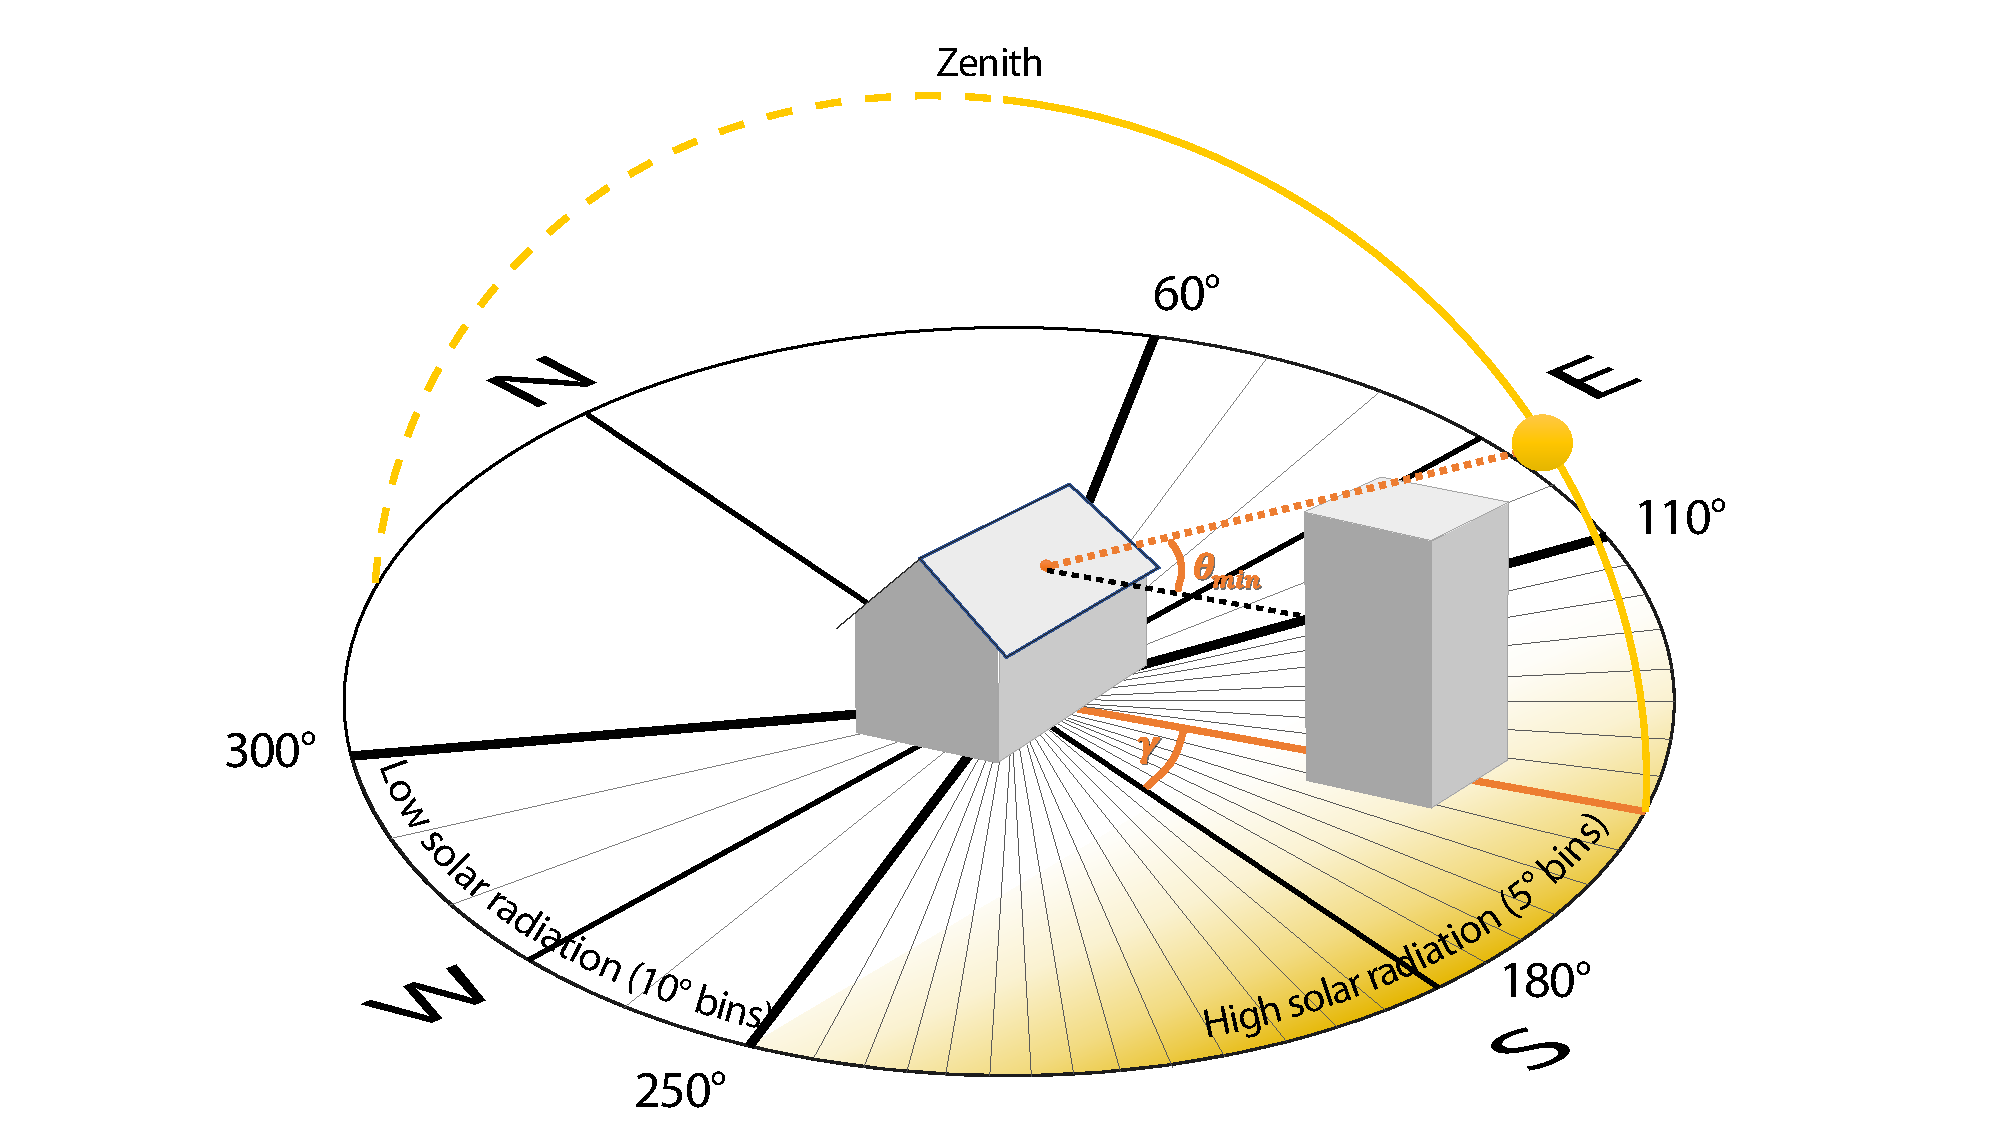
\includegraphics[trim=100 0 130 0, clip, width=.9\linewidth]{Figs/horizon.pdf}  
		\subcaption{}
        \label{figa:horizon_method}
	\end{subfigure}
	\begin{subfigure}[t]{.49\textwidth}
		\centering
		% include second image
		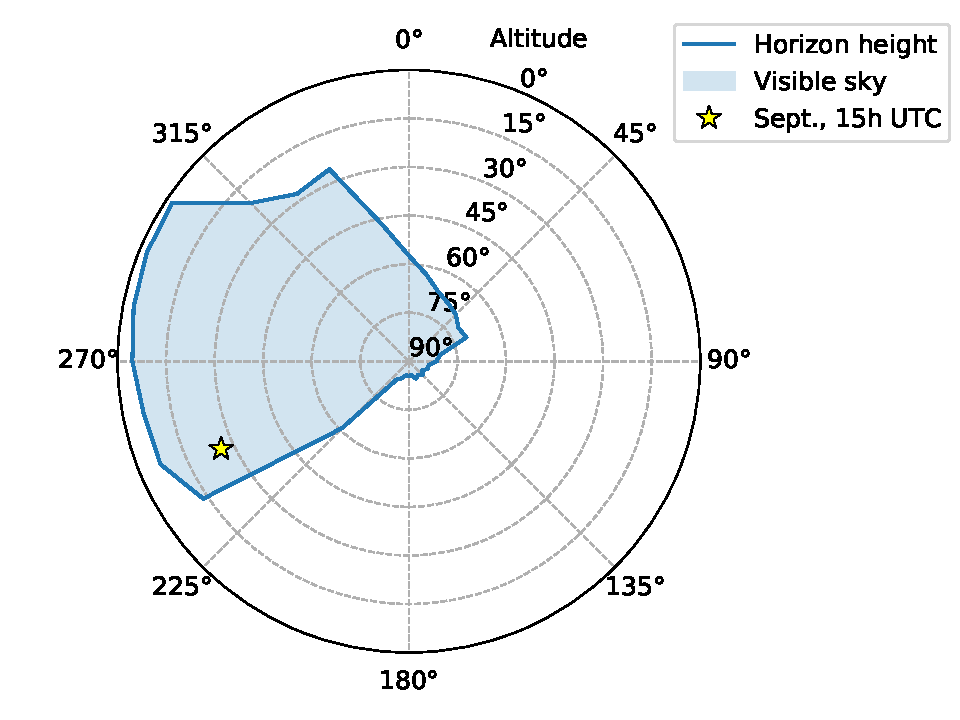
\includegraphics[width=\linewidth]{images/Figs/skyview_point_w_star.pdf}  
		\subcaption{}
		\label{figb:horizon_method}
	\end{subfigure}
	\caption{Horizon modelling for an example roof. (a) Conceptual graph with relevant horizon bins for quantification of shading effects, (b) polar plot of horizon height and visible sky proportion ($\mathit{SVF} = 0.3$), with an example sun position for Switzerland (September, 15h UTC).}
	\label{fig:horizon_method}
\end{figure}

\begin{figure}[htb]
	\centering
	\begin{subfigure}{.49\textwidth}
		\centering
		% include second image
		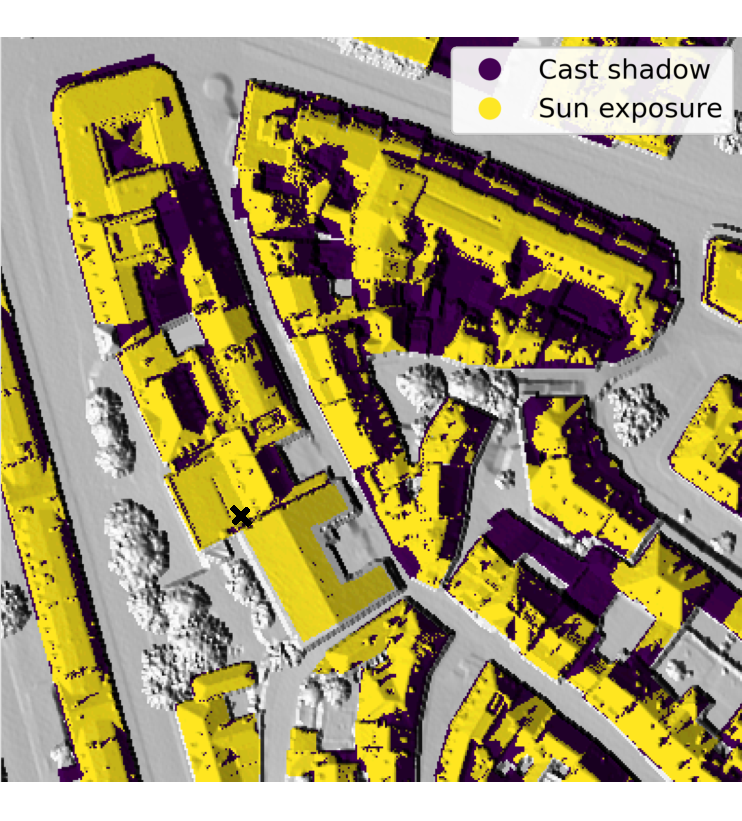
\includegraphics[height=.9\linewidth]{images/Figs/demo_vis_09_15h_w_cross.pdf}  
		\subcaption{}
        	\label{figa:raster_svf_ssh}
	\end{subfigure}
	\begin{subfigure}{.49\textwidth}
		\centering
		% include second image
		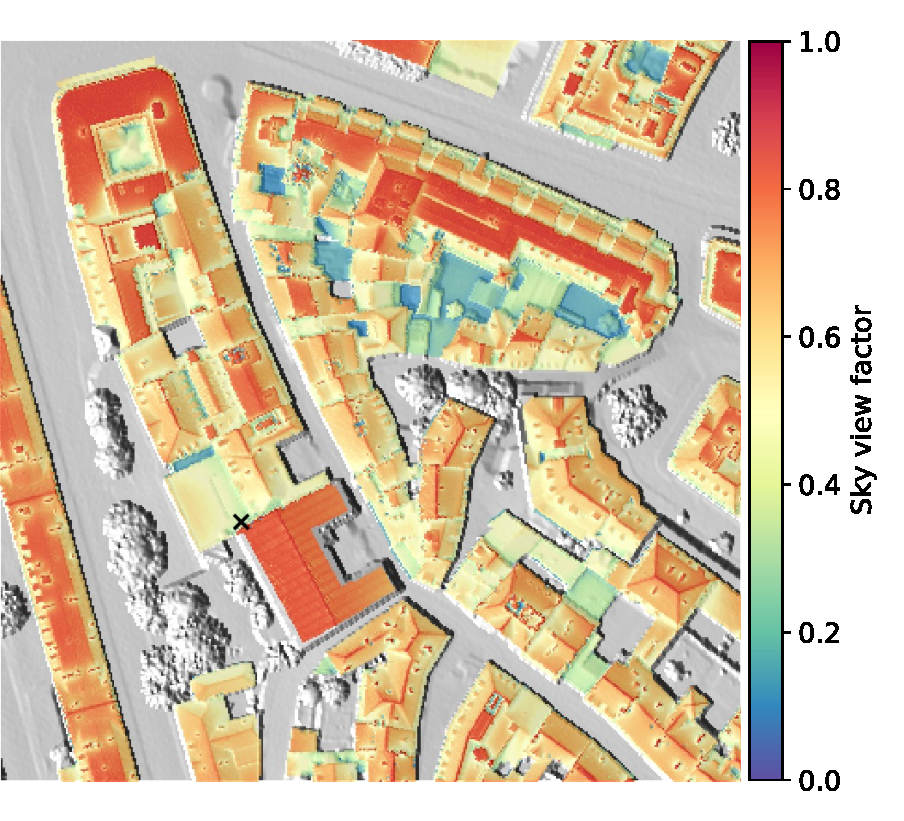
\includegraphics[height=.9\linewidth]{images/Figs/svf_w_legend.pdf}  
		\subcaption{}
        	\label{figb:raster_svf_ssh}
	\end{subfigure}
	\caption{Raster-based (a) cast shadows for one example hour (15h UTC in September, see star in Fig.\ref{figb:horizon_method}) and (b) sky view factor for an area of $200\times200$ m$^2$ in Geneva, Switzerland. The cross on the figures shows the point for which the horizon height is shown in Fig.\ref{figb:horizon_method}.}
	\label{fig:raster_svf_ssh}
\end{figure}

The computation of shading effects and the SVF follow a common 3D modelling approach, known as shadow casting \cite{levinson_solar_2009,desthieux_solar_2018}, ray tracing \cite{jakubiec_method_2013} or viewshed computation \cite{nguyen_incorporating_2012}. 
As shown conceptually in Fig.~\ref{figa:horizon_method}, a 3D model of the environment is used to obtain the horizon height for each aspect angle. 
%
This horizon height ($\theta_\mathit{min}$ in Fig.~\ref{figa:horizon_method}) describes the visible proportion of the sky for a specific aspect angle ($\gamma$ in Fig.~\ref{figa:horizon_method}), and may also be interpreted as the minimum sun elevation angle required to illuminate a given point. 
%
The horizon height for all aspect angles can be visualised as a polar plot, from which the SVF is derived as the visible sky fraction (Fig.~\ref{figb:horizon_method}). The polar plot further indicates whether the given point is shaded during a particular hour of the year based on the sun position (see star in Fig.~\ref{figb:horizon_method}).

While fisheye images \cite{calcabrini_simplified_2019} or LiDaR point clouds \cite{bill_3d_2016,jakubiec_method_2013} may be used for horizon computations, DEMs are by far the most widely used input data, as they enable the computation of horizon heights for an entire region \cite{suri_new_2004}.
Using a DEM to compute the horizon heights yields a set of raster maps, one for each azimuth angle.
From these, maps of cast shadows (Fig.~\ref{figa:raster_svf_ssh}) can be computed for any sun position, by selecting the horizon map corresponding to the sun azimuth angle and applying a binary filter to the raster values, setting all values below the sun altitude to 1 (sun exposure) and all values above the sun altitude to 0 (cast shadow).
%
The sky view factor is obtained from the same set of horizon maps, which are combined to obtain the SVF for each pixel (Fig.~\ref{figb:raster_svf_ssh}). The SVF is independent of the sun position and hence constant with time. 

While some studies compute PV potential at the level of individual pixels \cite{buffat_scalable_2018,ramirez_camargo_spatio-temporal_2015}, the results are often aggregated per building or roof surface \cite{assouline_quantifying_2017,assouline_large-scale_2018,klauser_solarpotentialanalyse_2016}. To aggregate shading effects or the sky view factor per roof, existing methods use 2D building or roof geometries, which are geospatially intersected with the raster maps to average all pixels within a given roof/building. This geospatial overlay further reduces the data storage requirements for the maps of shading and SVF, as all non-relevant areas for rooftop RPV potential are excluded.

In this work, we use the shadow casting and SVF computation method as detailed above. We use the open-source GRASS-GIS computational engine, which supports the computation of horizon heights \cite{suri_new_2004} and the sky view factor \cite{zaksek_sky-view_2011} and which is used in several of the reviewed studies \cite{ramirez_camargo_spatio-temporal_2015,nguyen_incorporating_2012,buffat_scalable_2018}. 
Further details regarding the implementation of the shading and SVF computation for scalability to the national scale for Switzerland are provided Appendix~\ref{app:shade}.

\begin{comment}
\subsection{Solar thermal heat generation}

The computation of the technical potential of a solar thermal collector is more complex to compute, as the solar thermal collector is typically coupled with a heat pump and a hot water tank. In the thermal application, the temperature of the collector and the ambience also play a larger role. Some studies still consider a constant efficiency value [27], while several studies suggest to consider temperature and incident irradiance [11], [28], [29].
\end{comment}

\subsubsection{Available area for solar panel installation}


Based on the an early study of RPV potential in Europe \cite{iea_potential_2002}, we identify three factors of the rooftop available area that are accounted for in different ways in the literature, namely (i) the total roof area, (ii) the roof utilisation and (iii) the roof exposure or suitability. 

The total roof area

The roof exposure/suitability

The roof utilisation

\begin{comment}
% For individual roofs, panels can be custom-fitted based on aerial photographs ~\cite{ordonez_analysis_2010} to realistically estimate the maximum available area, taking into account the rooftop geometry as well as any obstructing objects inhibiting the placement of solar panels (roof superstructures).
% Custom-fitting however is not scalable to entire cities or regions, requiring either image processing \cite{mainzer_assessment_2017} or high-resolution 3D building models \cite{engel_effiziente_nodate} for a detailed estimation of the available area.
% As the required input data is not available for many study areas and the computational time for these methods may be prohibitively high, approximative approaches are widely used in the literature.
These range from using standard tabulated factors based on expert opinions [26], statistical methods [7] and extrapolation techniques based on Machine Learning [3]. Assouline et al. [14] provide a detailed analysis of these methods. 

Focus primarily on radiation: Buffat, Desthieux; compute for individual systems: Calcabrini; 
Wegertseder: 25\% of useful roof area for res., 30\% for housing blocks, 50\% for high-rise towers

strzalka: manually excluding roofs with windows etc., otherwise using all areas

exclude small areas and strongly shaded areas: Hong (per time step)

Thus, many studies employ constant value methods \cite{assouline_estimation_2017}, which assume a constant ratio of available area. 
These ratios may be formulated with reference to territorial areas or population count \cite{izquierdo_method_2008,iea_potential_2002,wiginton_quantifying_2010,bodis_high-resolution_2019}, based on building prototypes \cite{wegertseder_combining_2016} or formulated as a constant fraction of individual roofs~\cite{portmann_sonnendach.ch:_2016}. 
In studies where detailed roof data is available through building cadastres 
Full rooftops \cite{bodis_high-resolution_2019}, rooftop avail area fraction ()

The geospatial algorithm is used to virtually install PV panels on the tilted roofs by projecting rectangular polygons onto these surfaces, as shown in Fig.~\ref{fig:panels}c. 
The starting point for this process are the roof polygons and superstructures (Fig.~\ref{fig:panels}a). Panels are installed on the grey areas in Fig~\ref{fig:panels}b, after superstructures (if applicable) and a buffer of 40cm are removed from the polygons~\cite{assouline_large-scale_2018}. The panels are installed in adjacent rows along the roof aspect, starting from the bottom left corner, as described in Algorithm \ref{alg:panels}. It is implemented using the python \texttt{geopandas} library \cite{kelsey_jordahl_geopandas/geopandas:_2019}.

Virtual PV panels were placed in both horizontal and vertical alignments, as no alignment has technical advantages over the other and both are widespread. The alignment that allows the higher number of panels to be installed on each roof is selected as final panel alignment. 
\end{comment}

\section{Shallow geothermal energy}
\label{geo_method}

ADD REFERENCES

As discussed in Section ~\ref{REN_CH}, ground-source heat pumps (GSHPs) using vertical closed-loop borehole heat exchangers (BHEs) are by far the most widely used technology to extract shallow geothermal energy in Switzerland \cite{blum_statistik_2016}.
%
Focusing on closed-loop BHEs, this section reviews state-of-the-art analytical models to assess the technical geothermal potential of shallow GSHPs. The technical potential is hereby defined as the heat energy that may be annually extracted from a field of BHEs by a GSHP system ($Q_{GSHP}$), which is computed as (cf. \cite{pahud_geothermal_2002}):
\begin{equation}
\label{eq:Q_field_method}
    Q_{GSHP}=q_{max} \times t_{op} \times H \times N_{BHE}
\end{equation}
where $q_{max}$ is the heat extraction rate from the boreholes (in W/m), $t_{op}$ is the operating time of the system (in h), $H$is the borehole depth (in m) and $ N_{BHE}$ is the number of installed BHEs.

To estimate the technical potential, the following factors must be taken into account: 
(i) The depletion of the ground when boreholes are placed too close to each other or too much heat is extracted; (ii) the sizing, geometry and material of the BHE tubes; (iii) the efficiency of the heat pumps that transfer the extracted heat to domestic heating and hot water applications. 
% The interaction of these components is a dynamical process that changes over time, which is described by the thermal response of the BHEs.

\begin{figure}[bt]
    \centering
    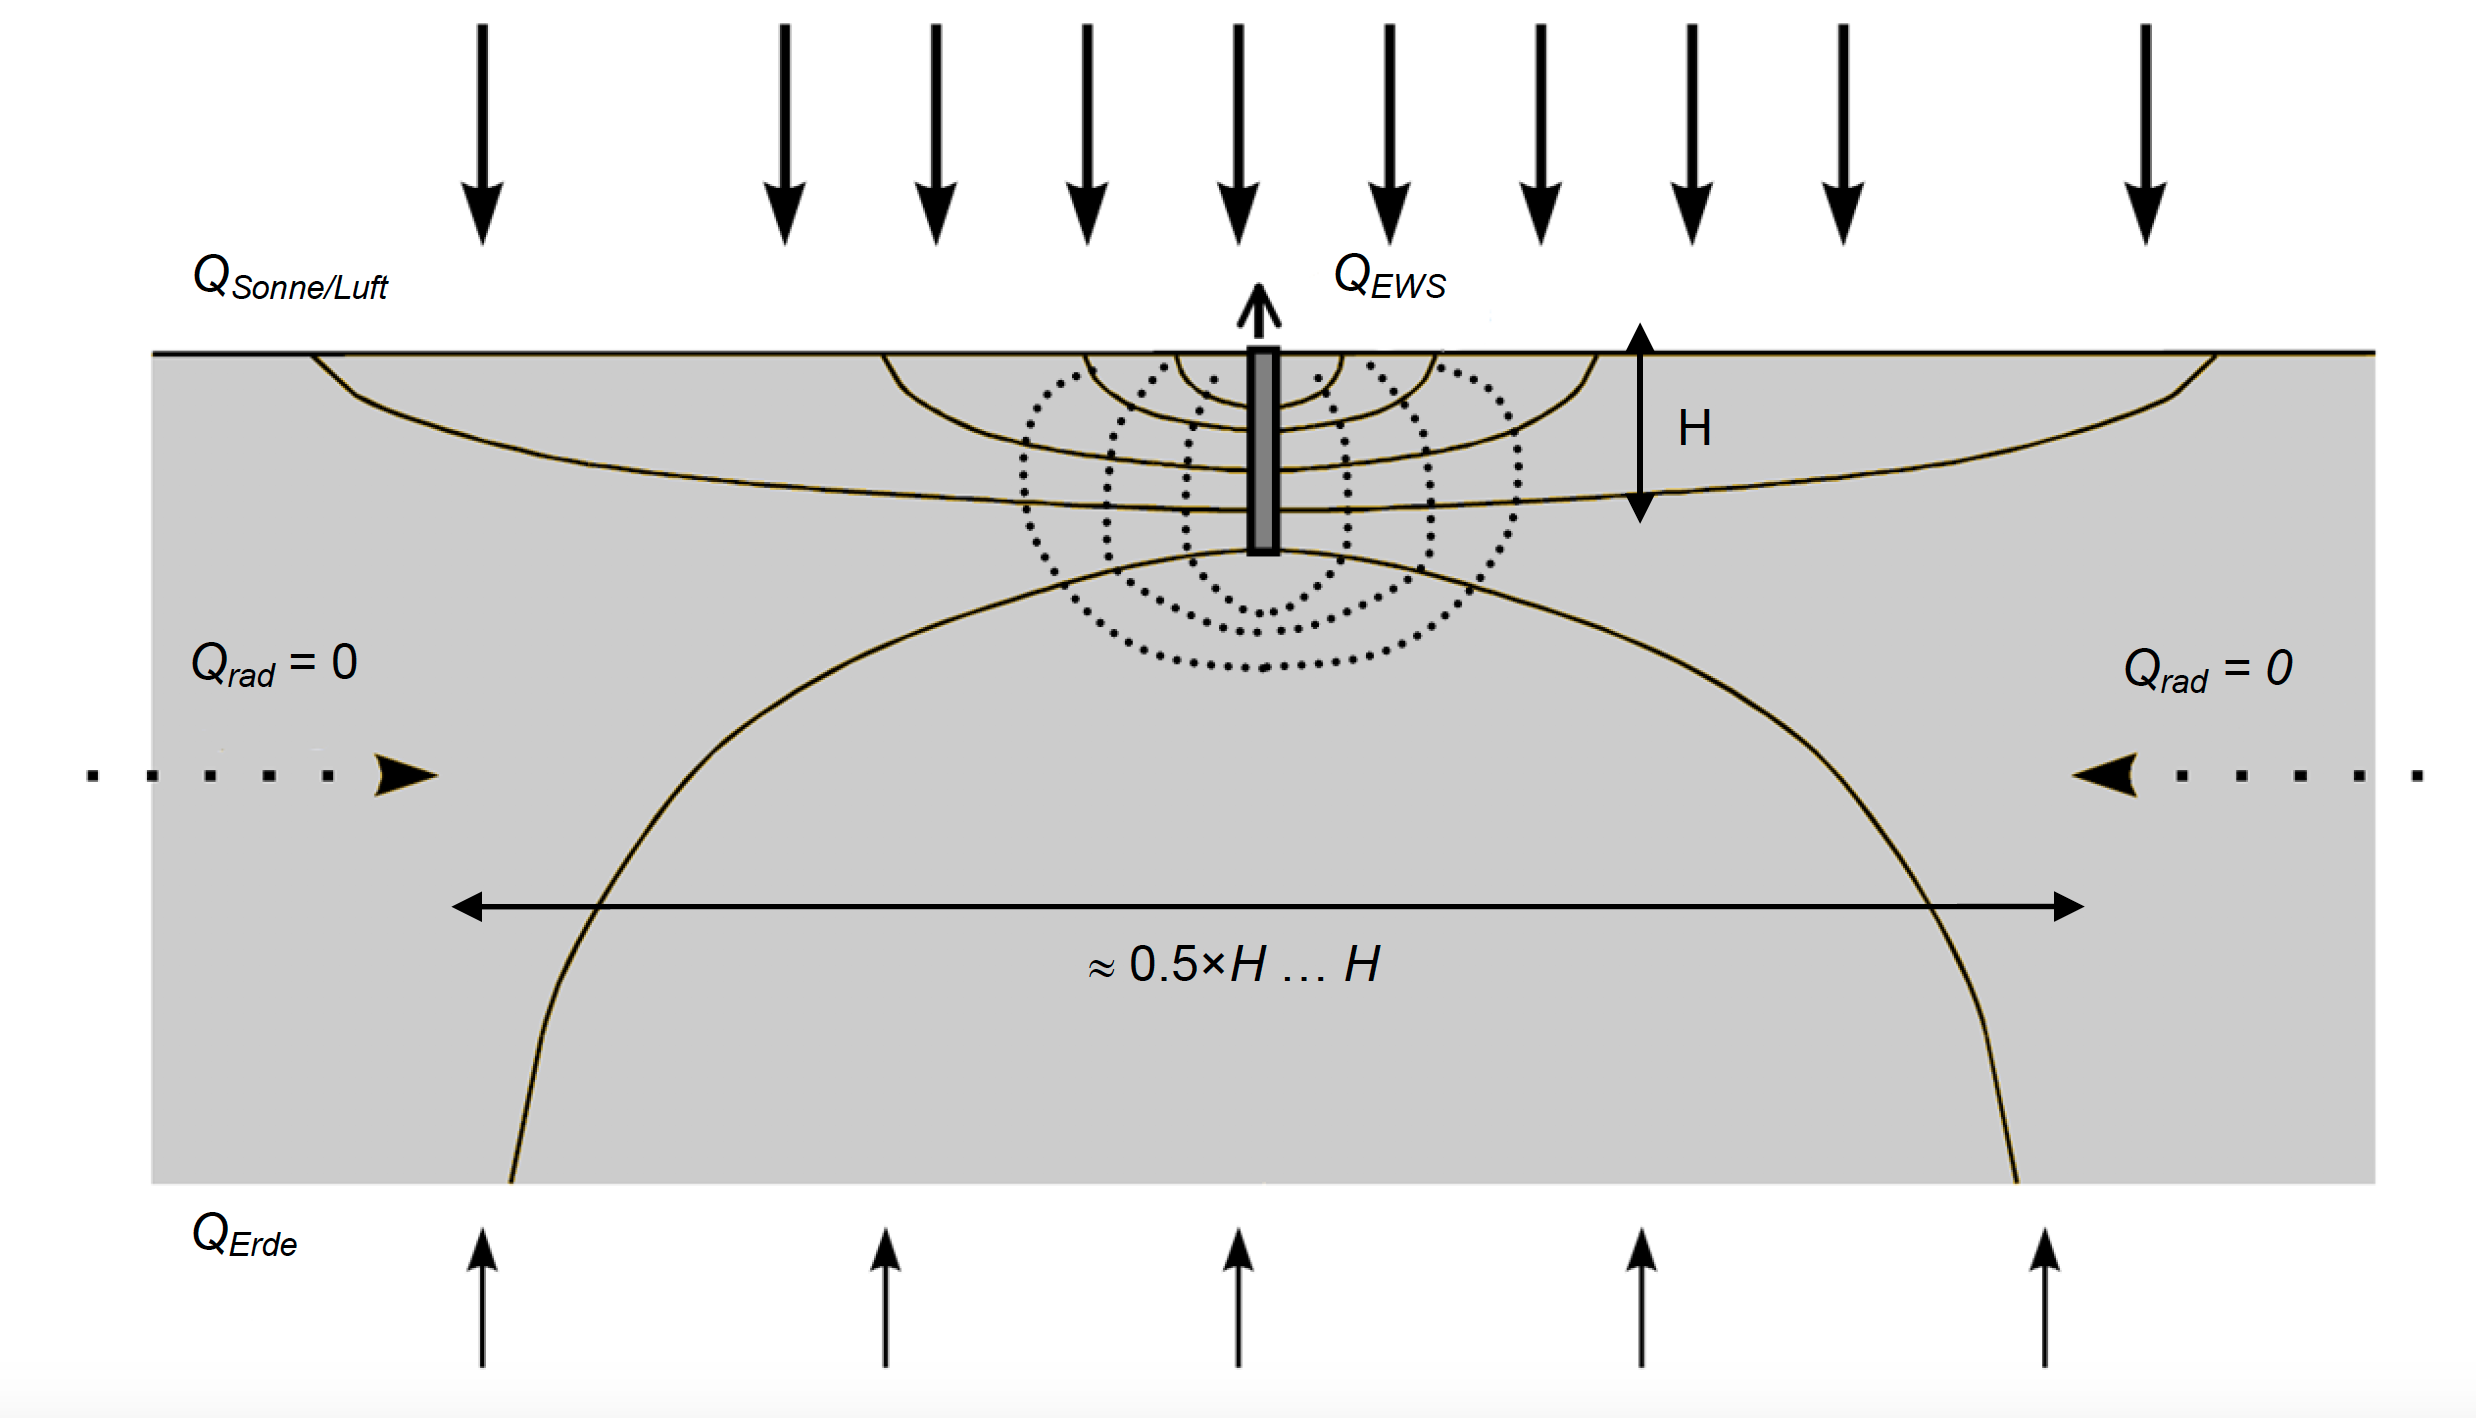
\includegraphics[width=0.7\linewidth]{Figs/BHE_layout.png}
    \caption[Single BHE installation and its effects on the temperature in the ground.]{Single BHE installation and its effects on the temperature in the ground. The arrows on the top indicate the natural heat flux from the environment, those on the bottom indicate the geothermal heat flux. The dashed lines are isothermal lines, while the continuous lines represent the heat flow in the stationary state. Source: \citet{wagner_erdsondenpotenzial_2014}}
    \label{fig:BHE}
\end{figure}

The depletion of the ground is driven by changes in the subsurface temperature, which occur when heat is extracted (or injected) at a faster rate than it is regenerated from the natural heat flux. This heat flux is caused by the heat in the earth's core (geothermal heat flux) and by the heat in the ambient air, as shown in Fig.~\ref{fig:BHE}.
As heat is extracted from the ground, so-called \textit{thermal plumes} are formed around the BHE (dashed lines in Fig.~\ref{fig:BHE}). Their magnitude and extent depends on the borehole design, particularly the depth and heat extraction rate, as well as on the thermal properties of the ground.
%
When boreholes are spaced too close to each other, thermal plumes may overlap, which causes \textit{thermal interference} between these boreholes and leads to an increased cooling of the subsurface. In this work, quantifying the thermal interference is of high importance, as thermal interference significantly reduces the potential borehole installation density.

Thermal interference between boreholes is assessed in the literature using an analytical model, developed by \citet{eskilson_thermal_1987}, which simulates the thermodynamic behaviour of BHEs based on the thermal ground properties as well as the sizing, geometry and material of the BHEs.
%
To formulate a technical potential for closed-loop GSHPs, related studies combine the this analytical model with norms for the current BHE design practice, using primarily the geothermal norms of the Association of German Engineers (VDI) \cite{vdi_vdi_2019} and the Swiss Society of Engineers and Architects (SIA) \cite{sia_sondes_2010}.
The parameters required for the analytical model and their values given by the SIA norm (relevant for Switzerland) will be introduced in Section~\ref{geo_params}.

Both the VDI and SIA norms require the BHEs to be designed and operated such that the mean temperature of the borehole fluid ($T_{mf}$) never drops below its freezing temperature ($T_\mathit{mf,min}=-1.5$ °C \cite{sia_sondes_2010}), such that:

\begin{equation}
\label{eq:T_mf_min}
T_{mf} \geq T_\mathit{mf,min} = -1.5 \text{°C}
\end{equation}

The variables in Eq.~\ref{eq:Q_field_method} ($q_{max}$, $t_{op}$, $H$, $N_{BHE}$) must hence be chosen such as to fulfil this technical requirement.
%
The relationship between these variables and the $T_{mf}$ is expressed by the borehole temperature profile, which describes the temperature changes inside and around a BHE.
A general model of this temperature profile, proposed by \citet{claesson_conductive_1988}, is introduced in Section~\ref{model_intro}, while Section~\ref{geo_models} details the analytical formulas used to estimate the thermodynamic processes in the ground.

While heat extraction is the dominant mode of operation of GSHPs in Europe \cite{lund_direct_2020}, GSHPs can also be used for heat injection, for example for space cooling applications \cite{kavanaugh_geothermal_2014}, whereby the same physical principles (Sections ~\ref{model_intro} and \ref{geo_models}) apply.
As heat injection is not addressed in the SIA or VDI norms, studies addressing the potential of GSHPs for heat injection \cite{aditya_environmental_2020,miglani_methodology_2018,michopoulos_potential_2011} use the standards of the American Society of Heating, Refrigerating and Air-Conditioning Engineers (ASHRAE) \cite{kavanaugh_geothermal_2014} for borehole sizing. For cooling-dominated systems, the temperature requirement from Eq.~\ref{eq:T_mf_min} is inverted, limiting the maximum fluid temperature $T_\mathit{mf,max}$:
\begin{equation}
\label{eq:T_mf_max}
T_{mf} \leq T_\mathit{mf,max}
\end{equation}
In addition to the BHEs, a GSHP system contains a heat pump (HP), which is used to transfer the heat extracted from the ground to the building heating or cooling systems (see Fig. \ref{fig:HP}), as these typically require different temperatures than those provided by the BHE. HPs have a high system efficiency, expressed through the coefficient of performance (COP), making GSHPs a very energy efficient technology for building thermal energy supply. Based on the COP, the heat supplied to the building heating ($Q_\mathit{heat}$) and cooling ($Q_\mathit{cool}$) systems is computed as \cite{kavanaugh_geothermal_2014}: 
\begin{equation}
\label{eq:COP_heat}
Q_\mathit{heat}=Q_\mathit{extr}\ \frac{COP_\mathit{heat}}{\left(COP_\mathit{heat}-1\right)}
\end{equation}

\begin{equation}
\label{eq:COP_cool}
Q_\mathit{cool}=Q_\mathit{inj}\ \frac{COP_\mathit{cool}}{\left(COP_\mathit{cool}+1\right)}
\end{equation}
where $Q_\mathit{extr}$ and $Q_\mathit{inj}$ are the extracted and injected heat from/to the BHEs and $COP_\mathit{heat}$/$COP_\mathit{cool}$ are the COPs for heating and cooling, respectively. In neighbourhood or redional-scale studies of the technical GSHP potential, the COP is typically chosen as a constant value \cite{miglani_methodology_2018,schiel_gis-based_2016,perego_techno-economic_2019}, while for studies at building scale, the COP often is modelled as a function of temperature \cite{fraga_heat_2018,liu_feasibility_2017,stene_residential_2005}.

\begin{figure}[bt]
    \centering
    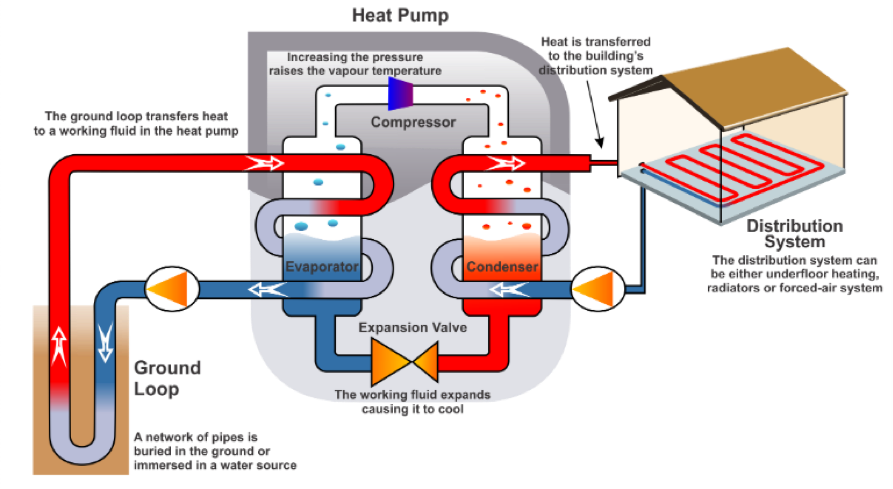
\includegraphics[width=0.7\linewidth]{images/Figs/GSHP.png}
    \caption{Working principle of a GSHP in heating cycle. Cold air is moved from the house to the heat pump, where it is heated from the compressed heat extracted from the ground. The ground loop liquid is cooled and transported back to the ground, where it is again heated. \cite{gns_science_n.z._geothermal_2016}}
    \label{fig:HP}
\end{figure}

\begin{comment}
This section provides an overview of the concept behind the estimation of the technical potential for borehole heat exchangers (BHE). It introduces the parameters used in the estimation (Section \ref{geo_params}) and summarizes the analytical methods for simulating the thermodynamic processes in the ground, which form the basis for the potential estimation (Section X, XX).

With appropriately dimensioned and spaced boreholes, a large-scale potential can be defined in $kWh/m^2$. This potential may be computed at annual temporal scales (using an annual mean heat extraction rate), at monthly scales (using the heat degree days as weighting function) or at hourly scales (using hourly load profiles).
The aim here is to define a maximum amount of energy that can be extracted from the ground without negatively affecting the long-term ground temperature. Energy demand is on purpose not taken into account. 
This is due to the fact that multiple operation modes exist, e.g. individual BHEs or entire fields that are connected to heat distribution networks. The separation between supply and demand also allows to simulate scenarios of "hybrid" systems, where the demand is covered by different sources.

This report summarizes the methods used to quantify the impact of a BHE installation on the short-term and long-term temperature in the ground, and consequently on the temperature of the heat extraction fluid inside the borehole. The case of a single borehole is shown in Fig.~\ref{fig:BHE}. The heat extracted by the borehole of length $H$ (in the center) leads to a temperature drop in the ground. This effect reduces with the distance $r$ to the center of the borehole, as indicated by the dashed lines that represent isothermal conditions. The temperature drop does not happen instantly, but the temperature reduces gradually over the years, until a \textit{steady state} is reached. In the steady state, the extracted heat equals exactly the energy flux from the environment (the air and sun on the surface, and the geothermal heat flux in the ground). The heat flow in this stationary state is shown by the continuous lines in Fig.~\ref{fig:BHE}. As a rule of thumb, the radius around the borehole which is impacted by the temperature drop in steady state is between $H/2$ and $H$. At distances further away from the borehole, the temperature drop can always be neglected \cite{pahud_geothermal_2002}, p. 49.

For typical BHE's of 100-250m, it takes a hundred years or more to reach this stationary state (see formula below). However, typical BHE installations are designed to be decommissioned after 50 years \citep{sia_sondes_2010}. In general, it is hence sufficient to fulfill the temperature requirement (see \ref{definition}) for the first 50 years of operation. This means that in practice it is still possible to install boreholes at distances of less than $H/2$, but numerical models are necessary to accurately quantify a distance which sustains a sufficient ground temperature in the planning horizon of 50 years.

The general intuition for the relationship between the spacing of boreholes, the length of the boreholes, the ground temperature and the heat extraction power is the following:
The closer boreholes are placed to each other, the stronger are they impacting each other, which results in a lower ground temperature. 
This lower ground temperature may cause the temperature of the heat carrier fluid to drop below the minimum allowed value; to prevent that, the heat extraction power must be reduced. 
In order to sustain a given heat extraction power and keep a close spacing between boreholes, the depth of the boreholes can be increased. This increases the ground volume from which heat is extracted, but may not be possible due to the ground materials or regulations. 
On the other side, a shorter borehole length means that heat is extracted at a higher rate, which also increases the temperature drop. This can be compensated by either reducing the heat extraction power (which lowers the efficiency of the system) or by increasing the borehole spacing.

\end{comment}

\subsection{Parameters}
\label{geo_params}
The parameters involved in the modelling of the thermodynamic behaviour of borehole heat exchangers can be divided into three groups: 

\begin{enumerate}
\item \textbf{Physical parameters} are determined by the geological and hydrological conditions of the ground, and are the subject of various large-scale studies \cite{signorelli_regional_2004,majorowicz_estimation_2009,tian_improved_2020}. Seasonal temperature variations in the ground are neglected, as boreholes typically have a length $> 50m$, which is far beyond the penetration depth of seasonal variations in the ground \cite{stauffer_thermal_2013}.

\item \textbf{Technical parameters} are derived from the materials and the technology of the BHEs. In this work, we use norm values found in the literature as constants and do not address the impact of variations in the technical parameters on the BHE potential.

\item \textbf{Design parameters} are related to the sizing of the BHEs and the borehole fields, in order to estimate a technical potential of GSHPs. These parameters and the impact of their variation on the GSHP potential are the main subject of this section. 
\end{enumerate}

We refer to $z$ (in m) for the depth in the ground, $r$ (in m) for the radial distance to the center of a BHE, $t$ (in hours or years) for the time and $T$ (in °C or K) for the temperature. 

\begin{table}[b]
\footnotesize
\caption{Physical parameters. Norm values and ranges for Switzerland are obtained from \citep{sia_sondes_2010}.}
\label{tab:phys_params}

\centering
\begin{tabular}{lllll}
\hline
\textbf{Symbol}             & \textbf{Unit} & \textbf{Description}           & \textbf{Formula}                                      & \textbf{Norm value / range (CH)} \\ \hline
$\lambda$                   & $W/mK$        & Thermal conductivity           &                                                       & $1-4$ (Plateau: $2-3$)           \\
$\alpha$                    & $m^2/s$       & Thermal diffusivity            & $\alpha = \frac{\lambda}{\rho C}$                     & $0.9-1.4 \times 10^{-6}$         \\
$\rho C$                    & $MJ/m^3K$      & Volumetric heat capacity       &                                                       & $1.2-3.5$ (Plateau: $2-2.5$)     \\ \hline
$T_g(z)$                    & $^\circ C$    & Undisturbed ground temperature &                                                       & \textit{Norm}: 10                         \\
$\frac{\Delta T}{\Delta z}$ & $K/m$         & Temperature gradient           & $T_g(z) = T_0 + z * \frac{\Delta T}{\Delta z} $       & Plateau: 0.03, Alps: 0.025       \\
$T_0$                       & $^\circ C$    & Surface temperature            &                                                       & \textit{Norm}: 8.5                        \\ \hline
$\dot{q}_{g}$               & $mW/m^2$      & Geothermal heat flow           & $\dot{q}_{g} = \lambda * \frac{\Delta T}{\Delta z}$   & $40-170$                         \\ \hline
\end{tabular}
\end{table}

\textbf{Physical parameters}. The physical parameters are listed in Table~\ref{tab:phys_params}. The \textit{thermal conductivity} $\lambda$ and \textit{thermal diffusivity} $\alpha$ are used in the analytical models. However, the geological properties of different types of rocks are typically provided as $\lambda$ and the \textit{volumetric heat capacity} $\rho C$. From these parameters, the thermal diffusivity is computed as \cite{pahud_geothermal_2002}:

\begin{equation}
    \alpha = \frac{\lambda}{\rho C}
\end{equation}
In the literature, the values for $\rho C$ and $\lambda$ are either derived from measurement data and interpolated using geostatistical kriging \cite{tian_improved_2020,munoz_estimating_2015} or Machine Learning~\cite{assouline_machine_2019}, obtained from 3D underground models \cite{garcia-gil_gis-supported_2015,groupe_de_travail_pgg_evaluation_2011} or, most frequently, mapped from tabulated values in the literature based on the present rock types~\cite{perego_techno-economic_2019,galgaro_empirical_2015,casasso_g.pot:_2016,gemelli_gis-based_2011}. An overview of typical thermal conductivity and heat capacity values for rock types found in Switzerland are provided in the SIA norm \cite{sia_sondes_2010} and by \cite{pahud_geothermal_2002}.

If hydro-geological data is available, the thermal conductivity can be adjusted to account for conductive heat transfer due to groundwater movement \cite{viesi_gis-supported_2018,assouline_machine_2019}, using the ground saturation level and the darcy velocity as input \cite{viesi_gis-supported_2018}. 
Advective heat transfer is neglected in the model proposed by \citet{eskilson_thermal_1987}.
Analytical models accounting for advective heat transfer have been used for example in \cite{garcia-gil_gis-supported_2015,alcaraz_advection_2016,alcaraz_t-i-ger_2017,attard_novel_2020}.
As the hyrdo-geological input data required for these advective-conductive models is not available at the regional scale for Switzerland, this thesis focuses on the conductive heat transfer model \cite{claesson_conductive_1988}. A similar approximation is applied in most related regional-scale studies, including\cite{perego_techno-economic_2019,galgaro_empirical_2015,casasso_g.pot:_2016,rivera_increased_2017,schiel_gis-based_2016}.

Another important physical parameter is the \textit{undisturbed ground temperature} $T_g(z)$. In particular, the temperature at half of the borehole depth ($z = H/2$) is of interest. If no data is available for estimating $T_g$ directly, it can be extrapolated from the \textit{surface temperature} $T_0$ and the \textit{temperature gradient} $\Delta T/\Delta z$: 
\begin{equation}
\label{eq:Tg}
    T_g(z) = T_0 + z * \frac{\Delta T}{\Delta z}
\end{equation}

\begin{figure}
    \centering
    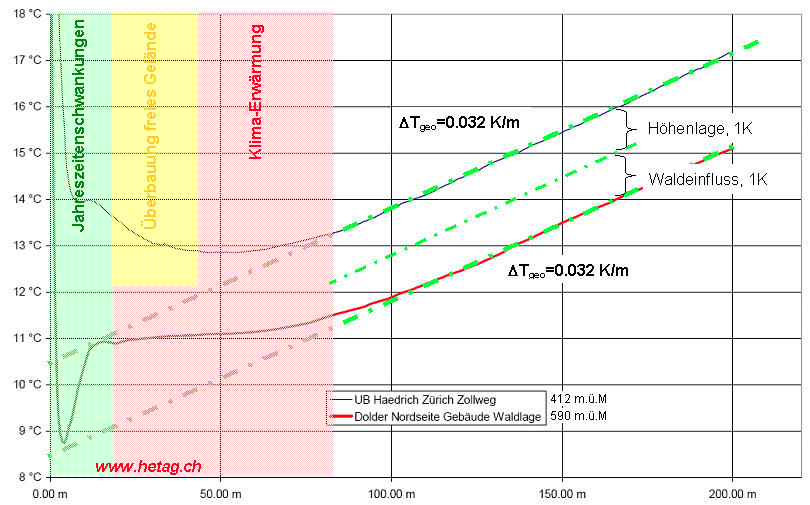
\includegraphics[width=0.6\linewidth]{Figs/ground_temperature.png}
    \caption[Example for the variation in ground temperature for two measurements of ground temperature in Zürich.]{Example for the variation in ground temperature for two measurements of ground temperature in Zürich, showing the influence of altitude (black line) and additional surface heating through the presence of forests (red line). Source: \citet{huber_bodentemperaturen_2014}.}
    \label{fig:T_ground}
\end{figure}
The $T_0$ can be obtained either interpolated based on measurements of the near-surface ground temperature \cite{assouline_machine_2019} or derived from measurements of the ambient temperature ($T_\mathit{amb}$). An analysis of different methods to determine $T_0$ is performed in \citep{signorelli_geoscientific_2004}. In the SIA norm, surface temperatures are  approximated from the mean annual $T_\mathit{amb}$ by adding an altitude-dependent term \cite{sia_sondes_2010}. As the actual $T_0$ may deviate from the approximated value (see Fig.~\ref{fig:T_ground} for an example), the SIA norm instructs the addition of a tolerance ($\Delta T$) of $- 1$ K heating for  $+1$ K for cooling applications.

\begin{comment}
Two examples for an unconsidered variation are shown in Fig.~\ref{fig:T_ground}. The presence of forests (red line) results in the ground temperature being approximately $1K$ lower than that expected from $\overline{T_{amb}}$. \citet{huber_bodentemperaturen_2014} states that, on the other hand, areas with high snow coverage may be up to $4K$ warmer than expected. The second example (black line) shows a case where the actual ground temperature is $1K$ higher than expected due to an altitude difference between the BHE and the weather station. In the Swiss plateau, this difference is approximately $0.47 K$ per $100m$ altitude increase with respect to the weather station \citep{huber_bodentemperaturen_2014}.
As the ground temperature in fact reflects the ambient temperature of the past, historic measurements should be used to determine the annual mean ambient temperature \citep{huber_bodentemperaturen_2014}. 
\end{comment}

While not being directly used in the analytical model of GSHPs, the (undisturbed) \textit{geothermal heat flow} $\dot{q}_{g}$ plays an important role in the quantification of geothermal resources, as it characterises the natural heat flow in the ground. It is given by \cite{huber_bodentemperaturen_2014}:

\begin{equation}
    \dot{q}_{g} = \lambda * \frac{\Delta T}{\Delta z}
\end{equation}
The geothermal heat flow is approximately constant across the outer crust of the earth, but may vary in mountain terrain \citep{huber_bodentemperaturen_2014}. The relationship may further be used to compute $\lambda$ or $ \frac{\Delta T}{\Delta z}$ if other data is unavailable. A map of geothermal heat flows in Switzerland is shown in Fig.~\ref{fig:q_geo}. It was created by Medici and Rybach in 1995 and updated by Sachs and Eberhard in 2010\footnote{Available at:\\ \url{https://opendata.swiss/de/dataset/geothermische-karte-der-schweiz-1-500000}}.

\begin{figure}
    \centering
    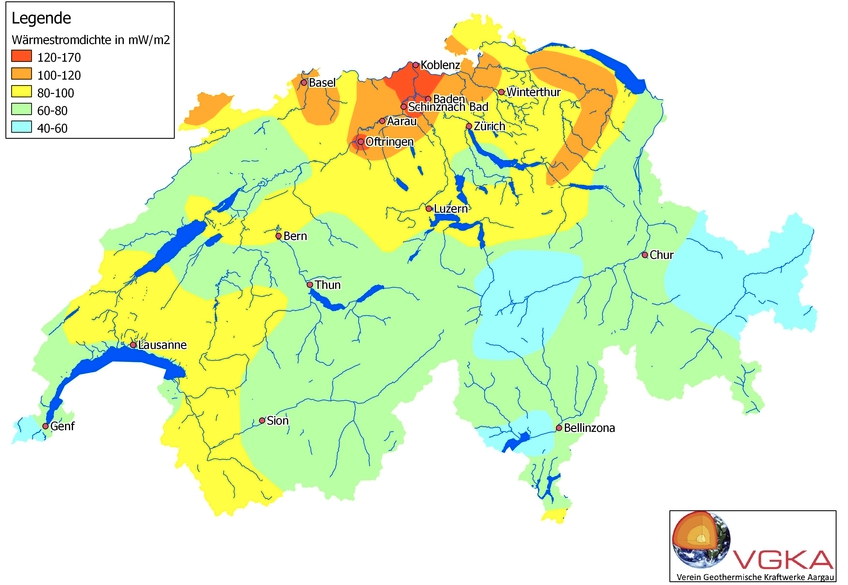
\includegraphics[width=0.6\linewidth]{Figs/q_geo.png}
    \caption[Map of geothermal heat flows in Switzerland]{Map of geothermal heat flows in Switzerland \citep{huber_bodentemperaturen_2014}.}
    \label{fig:q_geo}
\end{figure}

\begin{figure}[b]
    \centering
    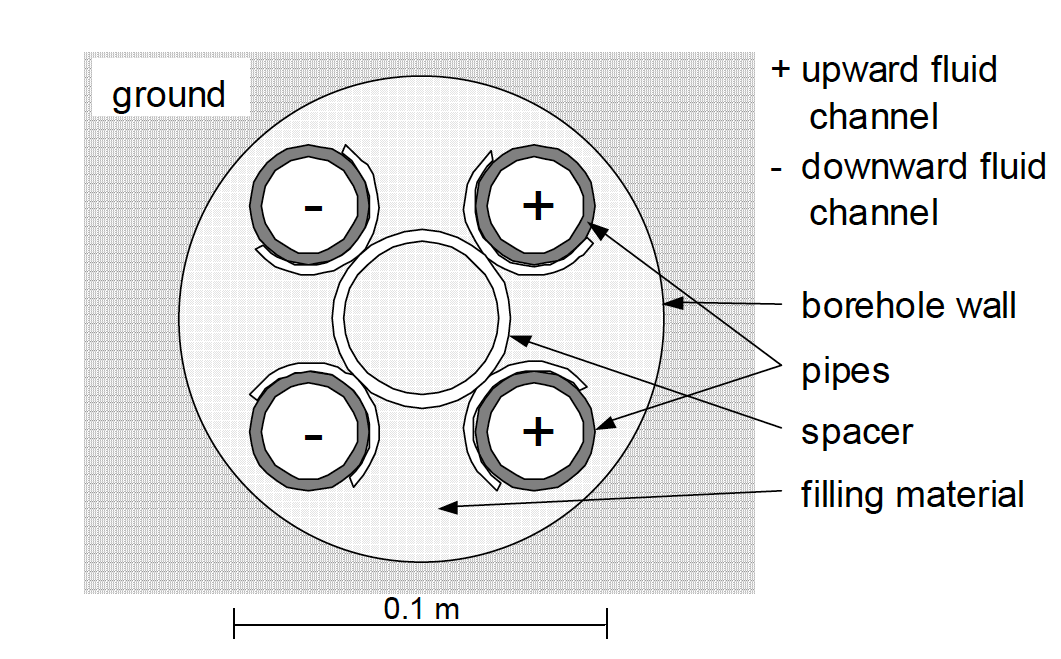
\includegraphics[width=0.4\linewidth]{Figs/BHE_tech.png}
    \caption[Cross-section of a duplex BHE layout.]{Cross-section of a duplex BHE layout \citep{wagner_erdsondenpotenzial_2014}.}
    \label{fig:BHE_cross-sec}
\end{figure}

\textbf{Technical parameters}. The technical parameters required to determine the technical geothermal potential are set as constant values in the literature (e.g. \cite{miglani_methodology_2018,rivera_increased_2017,zhang_critical_2017}). The $T_\mathit{mf,min}$ temperature is set in most reviewed studies to $-1.5^\circ C$ \citet{sia_sondes_2010}.
For $T_\mathit{mf,max}$, no unique value exists across the literature. Instead, \citet{kavanaugh_geothermal_2014} suggests to choose a $T_\mathit{mf,max}$ of $11 - 18$ °C above $T_g$ \cite{spitler_vertical_2016}.
Quantifying the temperature drop inside the borehole further requires knowledge of the borehole radius ($r_B$) as well as the effective thermal resistance of the borehole ($R_b^*$). A typical layout of a duplex system, the most common form of BHE installations (\cite{sia_sondes_2010}), is shown in Fig.~\ref{fig:BHE_cross-sec}. The thermal resistance is determined by the materials and the geometry of the BHE, which are analysed in detail in \citep{huber_erdwarmesonden_2005}. Table~\ref{tab:tech_design_params} summarises the range of parameters found in the literature and the SIA norm values (if applicable).

\textbf{Design parameters}. Two groups of design parameters are relevant to study the multi-fold effects between the geometry of a BHE field and the temperature in the ground, which is typically assessed after a planning horizon $t_{dim}$. 
The first group of parameters are related to the borehole geometry. These include the borehole length/depth ($H$), the horizontal distance between BHEs ($B$) and the distance between the top part of the BHE (where heat is extracted) and the ground surface ($D$). 

A second group of design parameters is related to the heat extraction from the borehole. It includes the heat extraction power ($Q_{HP}$), the maximum heat extraction rate ($q_{max}$), the operating time ($t_{op}$) and the duration of maximum operation ($t_{peak}$). The heat extraction power is related to the power rating of the heat pump (HP), whose typical values are shown in Table~\ref{tab:tech_design_params}. 
% In a large-scale study, however, $Q_{HP}$ is not a technical parameter, as the number of heat pumps in the system is undefined. 
The heat extraction rate is computed from $Q_{HP}$ and $H$ as given in Table~\ref{tab:tech_design_params}. Nominal curves for $q_{max}$ as a function of $\lambda$ and $\rho C$ ($q_{nom}$) are provided in \cite{sia_sondes_2010}. These curves can be approximated as (cf. \cite{sia_sondes_2010}):
\begin{equation}
\label{eq:q_nom}
    q_{nom} \approx \frac{T_g - T_{mf, min}}{11.5} \ \left( 10.6 \lambda + 11.2 + 2 \left( \frac{\lambda}{\alpha} - 2 \right) \right)
\end{equation}
% If these are used, $Q_{HP}$ needs to be computed by rearranging the equation for $q_{max}$. 
The operating time indicates the number of hours in which the heat pump is operating (with power $Q_{HP}$). The norm values, used throughout this work, depend on altitude and location \cite{sia_sondes_2010}.
%. It changes with altitude and location, and the nominal values are shown in Fig.~\ref{fig:t_q_norm}b. 
The duration of the peak extraction pulse ($t_{peak}$) measures the maximum time of non-stop operation of the HP, which impacts the maximum temperature drop in the BHE and is usually taken as 1, 5 or 10 days \cite{pahud_geothermal_2002}.

\begin{table}[t]
\footnotesize
\caption{Technical and design parameters. Norm values are given in \citep{sia_sondes_2010}, while other parameters are obatined from related studies \citep{pahud_geothermal_2002, wagner_erdwarmesonden._2019, claesson_conductive_1988}.}
\centering
\resizebox{\textwidth}{!}{%
\begin{tabular}{lllll}
\hline
\textbf{Symbol} & \textbf{Unit} & \textbf{Description}                   & \textbf{Formula}                                        & \textbf{Norm value / range (CH)} \\ \hline
$T_{f, min}$    & °C   & Minimum mean fluid temperature         & $T_{f} = \frac{T_{in} + T_{out}}{2}$                    & \textit{Norm}: $- 1.5$           \\
$r_b$           & m           & Borehole radius                        &                                                         & $0.055-0.07$                      \\
$R_b^*$         & mK/W        & Effective borehole resistance          &                                                         & $0.08-0.1$                       \\ \hline
$H$             & m           & Borehole depth                         &                                                         & \textit{Norm}: $100$ (mostly $50-200$)          \\
$D$             & m           & Distance between $z=0$ and BHE outlet  &                                                         & $2-5$                              \\
$B$             & m           & Spacing between BHEs                   &                                                         & $>5$ (no effect for B $>$ H)     \\ \hline
$Q_{HP}$        & W           & Heat extraction power during operation &                                                         & $4500-8400$                      \\
$q_{max}$       & W/m         & Maximum heat extraction rate           & $q_{max} = \frac{Q_{HP}}{H}$                            & \textit{Norm} ($q_{nom}$): $20-55$           \\
$t_{op}$        & h           & Annual operation time                  &                                                         & \textit{Norm}: $1850$  \\
$t_{peak}$      & h           & Duration of maximum extraction pulse   &                                                         & $1 - 10$ days                    \\ 
\hline
$t_{dim}$       & years           & Planning horizon for dimensioning the BHE   &                                                         & $50$                    \\ 
\hline
\end{tabular}
}
\label{tab:tech_design_params}
\end{table}

\begin{comment}
\begin{figure}[b]
\centering
\begin{subfigure}{.48\textwidth}
  \centering
  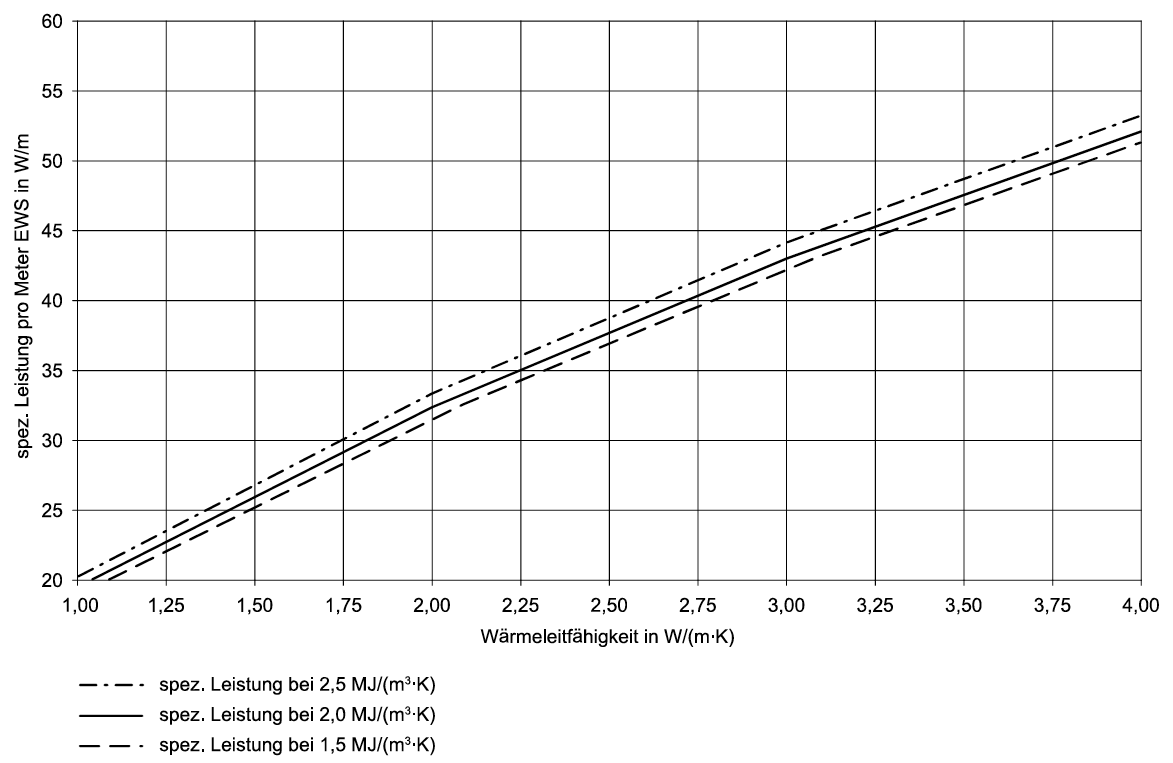
\includegraphics[width=.96\linewidth]{Figs/q_max_norm.png}  
\end{subfigure}
\begin{subfigure}{.48\textwidth}
  \centering
  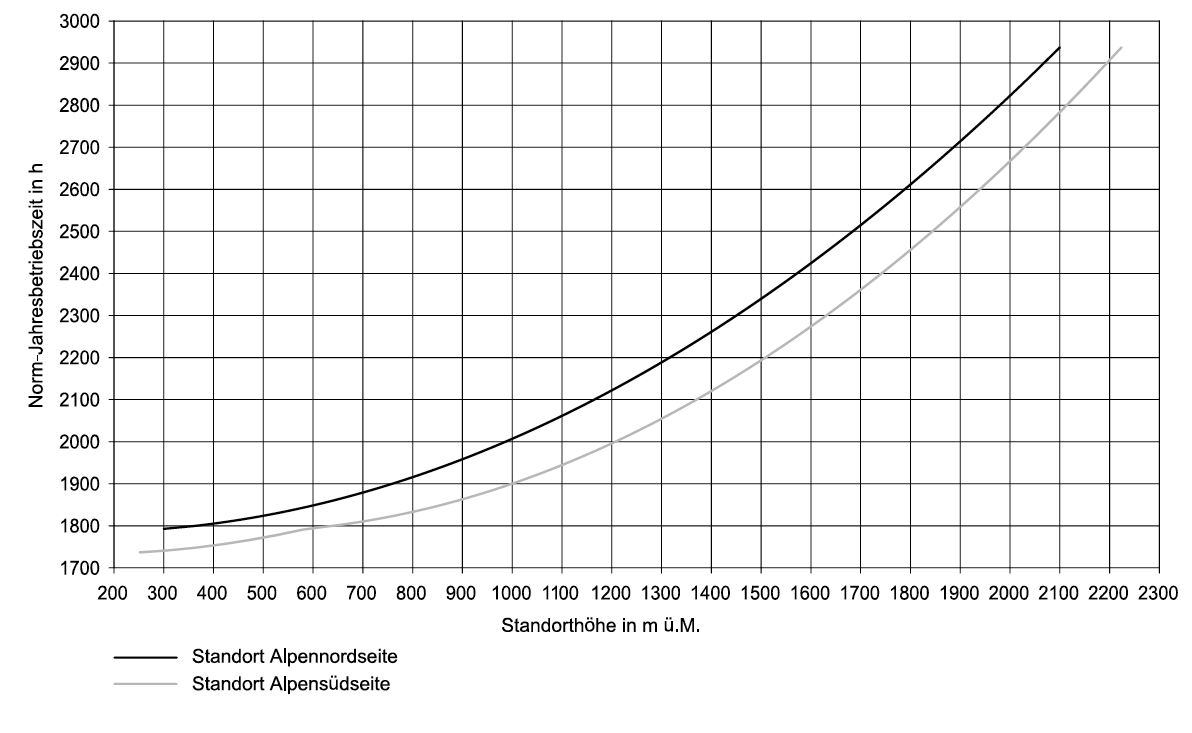
\includegraphics[width=\linewidth]{Figs/t_op_norm.png}  
\end{subfigure}
\caption{a) nominal heat extraction rate ($q_{max}$) for a duplex BHE (32mm) at $H=100m$, $T_g=10$, $t_op = 1850h$ as a function of $\lambda$ and $\rho C$, b) nominal operating time ($t_{op}$) as a function of altitude north and south of the alps \citep{sia_sondes_2010} (Fig. 7 \& 10).}
\label{fig:t_q_norm}
\end{figure}
\end{comment}

\subsection{Temperature profile of a BHE installation}
\label{model_intro}

To quantify the temperature field of a BHE, we distinguish between the processes inside and outside the BHE. The temperature drop inside the BHE, i.e. between the heat carrier fluid at mean temperature $T_f$ and the borehole wall at temperature $T_b$, is a function of the heat extraction rate and the effective thermal resistance of the borehole, such that \citep{claesson_conductive_1988}:

\begin{equation}
\label{eq:T_b}
    T_b(t) - T_f(t) = q_{max}*R_b^*
\end{equation}

\begin{comment}
The inlet temperature of the fluid may be obtained from the following equation \citep{pahud_geothermal_2002}, p. 43:

\begin{equation}
    q_{max} * H = \dot{m} * cp_f * (T_{f, out} - T_{f, in})
\end{equation}

where $Q_{HP}$ is the heat extraction power of the heat pump, $\dot{m}$ is the mass flow rate of the fluid (in $kg/s$), $cp_{f}$ is the thermal capacity of the fluid (in $J/kgK$) and $T_{f,in}$ and $T_{f,out}$ are the inlet and outlet temperatures.
\end{comment}

The temperature at the borehole wall $T_b$ differs from the undisturbed ground temperature $T_g$ by a temperature drop $\Delta T_b$. It varies with depth ($z$), so the average value along the borehole may be obtained by numerical integration ($z = \overline{z}$) or, in a simplified way, by taking $z = H/2$. The borehole wall temperature $T_b$, with $r = r_b$, is hence computed as:
\begin{equation}
    T_b(z, t) = T_g(z) - \Delta T_b(z, t)
\end{equation}

\begin{figure}
    \centering
    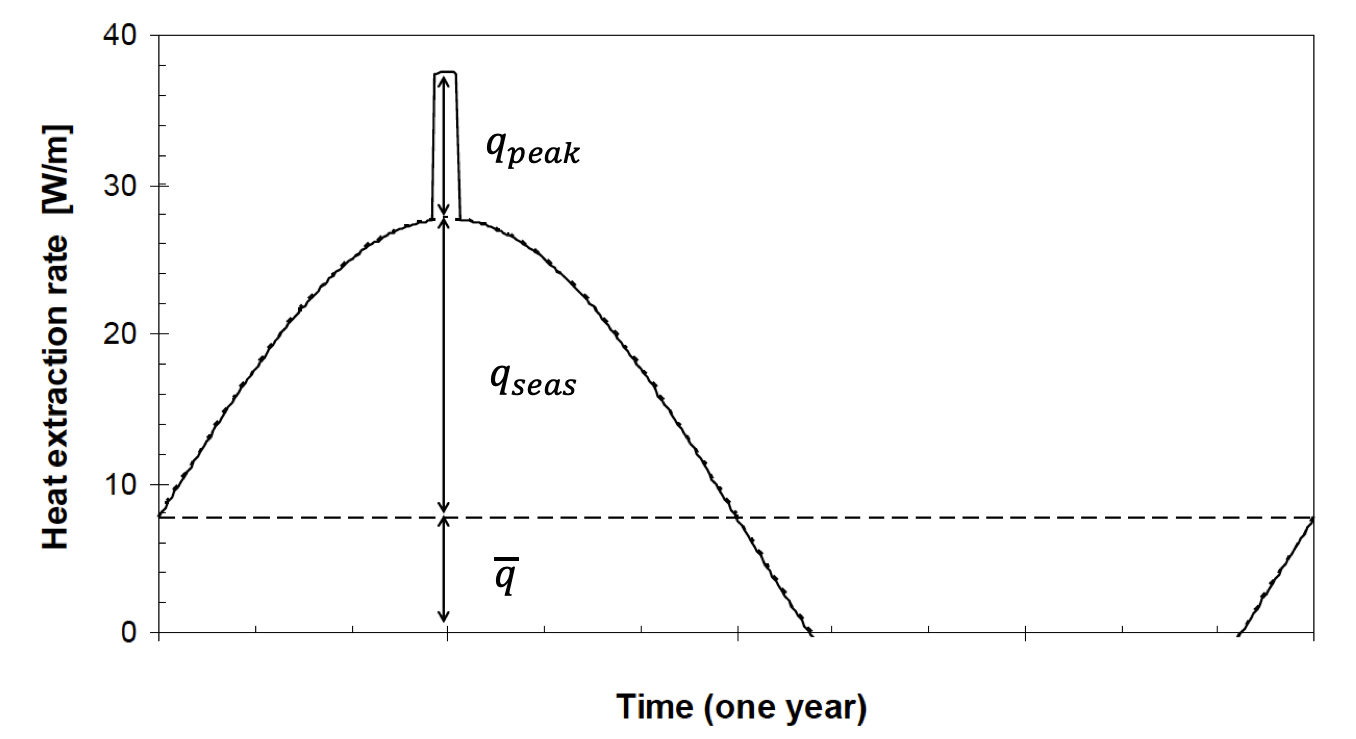
\includegraphics[width=.6\linewidth]{Figs/q_seasonal.png}
    \caption{"Simplified heat extraction rate evolution for a typical year (constant + periodic + pulse)" \citep{pahud_geothermal_2002}.}
    \label{fig:q_seasonal}
\end{figure}

The analytical model proposed by \citet{eskilson_thermal_1987} is based on the principles of temporal and spatial superposition, which assumes that $\Delta T_b$ is the sum of the temperature drops due to heat extraction pulses of different duration and from any neighbouring borehole, whereby boreholes at distances greater than $H/2$ can be neglected \cite{pahud_geothermal_2002}.

The principle of temporal superposition implies that $\Delta T_b(z, t)$ can be modelled as a long-term (\textit{LT}), a seasonal (\textit{seas}) and a short-term (\textit{peak}) component \citep{claesson_conductive_1988}, as shown in Fig.~\ref{fig:q_seasonal}.
%
% A method to model these effects, shown in Fig.~\ref{fig:q_seasonal}, is suggested in  and summarized in \cite{pahud_geothermal_2002}. 
%
Long-term effects are represented by a constant heat extraction rate $\overline{q}$, which is typically assessed for a planning horizon ($t_{dim}$) of 20 or 50 years \cite{pahud_geothermal_2002,miglani_methodology_2018}. 
Seasonal effects are represented as a sinusoidal heat extraction with peak rate $q_\mathit{seas}$ and period $t_\mathit{seas}$ of 1 year.
% , so that the annual integral is zero.
The peak extraction, which occurs at maximum seasonal extraction, has a duration $t_\mathit{peak}$ (typically 1-10 days). The energy extracted from this pulse is neglected \cite{claesson_conductive_1988}. 
To obtain $\Delta T_b$, each heat extraction rate is multiplied with a respective thermal resistance ($R_{LT},R_\mathit{seas},R_\mathit{peak}$) \cite{claesson_conductive_1988}:
\begin{equation}
\label{eq:dT_b}
    \textstyle \Delta T_b(z, t) = \overline{q} * R_{LT}(z, t) + q_{seas} * R_{seas}(z,t) + q_{peak} * R_{peak}(z, t)
\end{equation}
where
\begin{equation*}
    \overline{q} = \frac{t_{op}}{365*24} * q_{max}, \quad q_\mathit{seas} = w_\mathit{seas} * q_{max}, \quad q_\mathit{peak} = q_{max} - \overline{q} - q_\mathit{seas}
\end{equation*}
and $w_\mathit{seas}$ is the seasonal system load, given as a dimensionless constant.

Equation~\ref{eq:dT_b} can be used to simulate the temperature variation at the borehole wall for any time $t$. 
For GSHP system sizing and to assess the potential long-term heat extraction from the ground, the worst-case $\Delta T_b$ and consequently the lowest $T_{mf}$ (or highest, for heat injection) must be calculated and substituted in Eqs.~\ref{eq:T_mf_min} (heat extraction) or \ref{eq:T_mf_max} (heat injection).
To obtain the $T_{mf}$, the temperature drop along the entire borehole is of interest, denoted as $H$ (the borehole depth).
Using this notation, a combination of Eqs.~\ref{eq:T_b}-\ref{eq:dT_b} gives the following equation for the lowest/highest $T_{mf}$:
\begin{equation}
   T_{mf}(t) =  \textstyle T_g\left(\frac{H}{2}\right) - \overline{q} * R_{LT}(H, t_{dim}) - q_{seas} * R_{seas}(t_\mathit{seas}) - q_{peak} * R_{peak}(t_\mathit{peak}) - q_{max}*R_b^*
\end{equation}
For reasons explained in Section~\ref{app:models}, only the $R_{LT}$ is a function of the borehole depth $H$.
This equation is valid for the cases of heat extraction (e.g. space heating) and heat injection (e.g. space cooling). The difference between the two modes of operation is that the heat extraction rates ($q$) are positive for heat extraction and negative for heat injection and that their magnitude may vary depending on the length of the heating/cooling seasons and the respective demand.

The principle of spatial superposition implies that the temperature drops due to the heat extraction from neighbouring BHEs is added to the temperature drop at the borehole wall. 
%
As the seasonal and peak effects are of a short duration and have a penetration radius of less than the minimum borehole distance $B_{min} = 5$m \cite{pahud_geothermal_2002}, the seasonal and peak components of neighboring boreholes hence do not interfere with each other.
%
% and can be approximated as functions of the technical and physical parameters only (i.e. $r_b, \lambda, \alpha$). Their penetration radius is a few meters and lies below the minimum borehole distance $B_{min} = 5m$, so seasonal and peak effects of neighboring boreholes do not interfere with each other. Consequently, $R_{seas}$ and $R_{peak}$ are "quasi-constants" in the large-scale geothermal potential estimation. The analytic formulas for both components are given in Section~\ref{seas_peak}. 
%
The long-term temperature drop ($\Delta T_{LT}$), however, may be impacted by surrounding boreholes. Fig.~\ref{fig:T_field} shows the long-term $\Delta T$ for different times, a) at the borehole wall as a function of $z$ and b) integrated along $z$ (denoted as $\overline{z}$ in Fig.~\ref{fig:T_field}b) as a function of distance to the borehole. Most of the temperature drop occurs during the first 10 years of operation, while the temperature drop after the planning horizon of 50 years is small.

\begin{comment}
Consequently, the long-term thermal resistance of the ground at the wall of borehole $i$ consists of the thermal resistance caused by this borehole, and the thermal resistances caused by any surrounding boreholes, such that:

\begin{equation}
\label{eq:R_field}
    R_{LT,i}(\overline{z}, t_{dim}) = R_{LT}(\overline{z}, t_{dim}, r_b) + \sum_{i \neq j} R_{LT}(\overline{z}, t_{dim}, r_j)
\end{equation}
where $R_{LT}(\overline{z}, t_{dim}, r_b)$ denotes the long-term thermal resistance of borehole $i$ at its borehole wall ($r_b$) and $R_{LT}(\overline{z}, t_{dim}, r_j)$ denotes the thermal resistance at a distance $r_j$ from any surrounding borehole.
\end{comment}
% While in most studies of GSHP potential the borehole depth and dimensioning horizon are considered as constants \cite{}, this formulation

\begin{comment}
% Figure~\ref{fig:T_field}a shows that the approximation of $z=H/2$ quantifies the worst-case temperature drop along the borehole. The rules of thumb given in \citep{pahud_geothermal_2002}, p. 50, state that the temperature drop is small at a horizontal distance of $r>H/2$ from the center of the BHE, and negligible for $r>H$. This is confirmed by Fig.~\ref{fig:T_field}b. 
We refer to the long-term temperature drop as $\Delta T_{LT}$ and include $r$ as variable, as also distances $r>r_b$ are of interest:

\begin{equation}
    \Delta T_{LT}(r, z, t) = \overline{q} * R_{LT}(r, z, t)
\end{equation}
\end{comment}

\begin{figure}
    \centering
    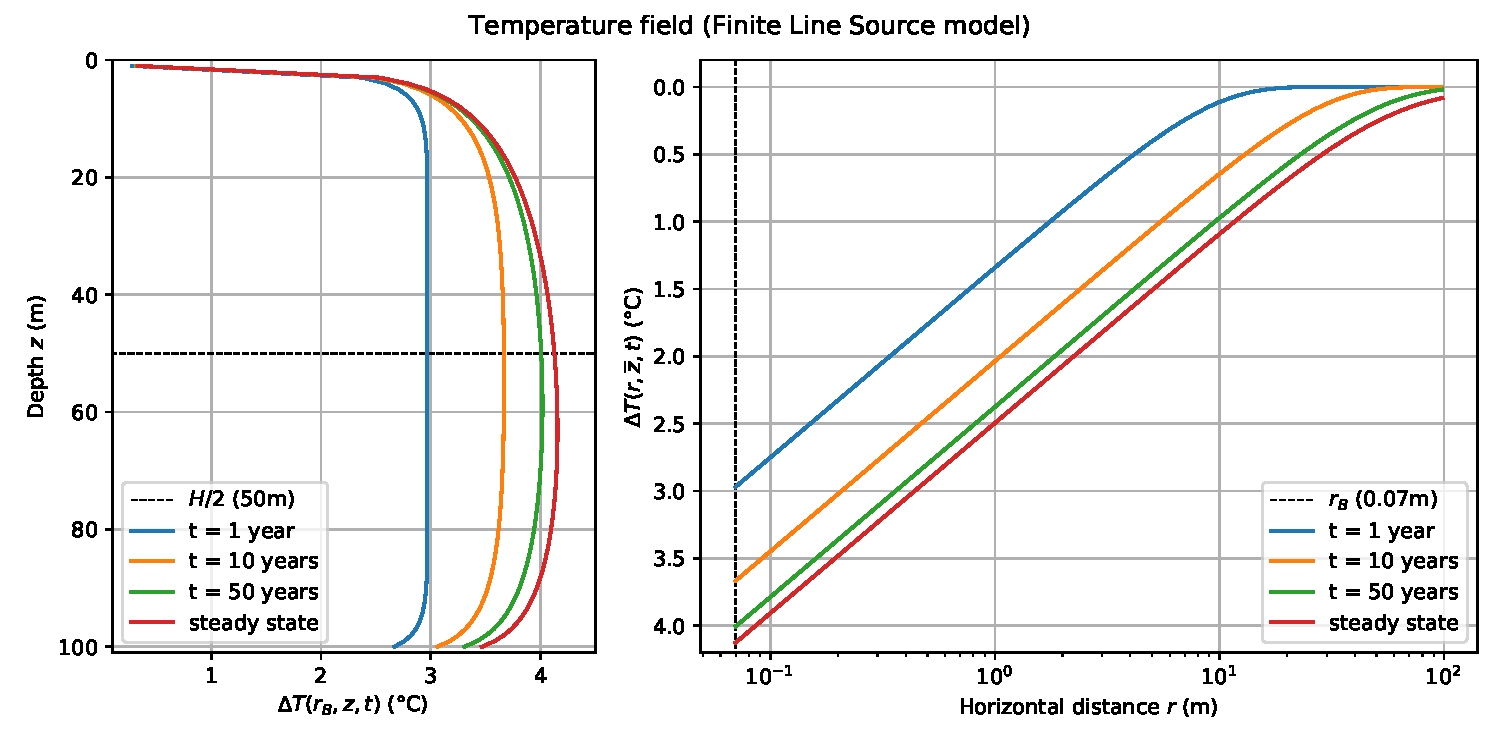
\includegraphics[width=.9\linewidth]{Figs/temp_field_FLS.pdf}
    \caption{a) Long-term variation of the ground temperature at the borehole wall ($\Delta T_{LT}(r_b, z, t)$) as a function of depth ($z$), b) Integration of $\Delta T_{LT}(r_b, z, t)$ along $z$ ($\Delta T_{LT}(r, \overline{z}, t)$) as a function of distance to the BHE ($r$).}
    \label{fig:T_field}
\end{figure}

\subsection{Analytical models for thermal resistance}
\label{geo_models}
\label{app:models}

In the model of \citet{claesson_conductive_1988}, the heat transfer of a BHE is modelled with good accuracy as a purely conductive process in a homogeneous medium. 
% This means that convective heat transfers are negligible. 
This implies that the thermal conductivity $\lambda$ of stratified ground with multiple layers may be approximated as a weighted average of the properties of the layers. 
\citet{claesson_conductive_1988} also argue that the undisturbed ground temperature $T_g(z)$ along the borehole can be approximated without loss of accuracy by the undisturbed ground temperature at half the borehole depth. 

To ease the notation fot the computation of thermal resistances ($R$), \citet{eskilson_thermal_1987} has introduced the concept of \textit{g-functions}. They are are dimensionless step-response functions characterizing the thermodynamic behaviour of the ground, from which $R$ is obtained as \cite{eskilson_thermal_1987}:

\begin{equation}
    R = \frac{1}{2 \pi \lambda} \, \mathrm{g}\left( \frac{t}{t_s}, \frac{r}{H} \right), \quad \frac{t}{t_s} > 0
\end{equation}

The g-function is a function of the ratio between the time $t$ and the BHE's time constant $t_s$, as well as the ratio between the horizontal distance to the BHE center $r$ ($r_b$ for a single borehole) and the borehole length $H$. The ratio $t/t_s$ may also be referred to as Eskilson's number (Es) \citep{pahud_geothermal_2002}. 
% For simplicity, only the variables (i.e. $r, z, t$, not the parameters $t_s, H$) are indicated in the argument of the g-function (where relevant). 
The time constant $t_s$, typically between $35-140$ years, is defined as:

\begin{equation}
    t_s = \frac{H^2}{9 \alpha}
\end{equation}
The time constant marks the transition from the transient state, in which ground temperatures are decreasing logarithmically, to the steady state, which represents the new thermal equilibrium of the ground with a constant heat extraction (red line in Fig.~\ref{fig:T_field}).
Since the dimensioning horizon of BHEs lies typically below $t_s$, the transient state solutions for the heat transfer equation are of primary interest for the modelling of BHEs. A complete overview of transient and steady-state models is provided by \citet{pahud_geothermal_2002}.
% This steady state is fully reached when $\ln{(t/t_s)} = 2$, i.e. $t_{ss} = e^2 t_s \approx 7.5 t_s$ \citep{wagner_erdsondenpotenzial_2014}. 

\subsubsection{Finite Line Source (FLS)}
The BHE is modelled by \citet{claesson_conductive_1988} as a finite line source (FLS) of length $H$. The analytical model is
% The FLS describes the most accurate analytic model used in the literature. It is 
a solution to the heat conduction equation that satisfies the boundary conditions $T(r, z=0, t=0) = 0$. 
The temperature changes along the BHE are modelled by the integral of the FLS solution along the vertical axis ($z$).
A computationally efficient solution for this integral (in transient state) has been proposed by \citet{claesson_analytical_2011}:
% The g-function of the transient solution is given by \citep{pahud_geothermal_2002}:
%To compute the mean $R_{LT}$ along the borehole length at a radial distance $r$ from the BHE, we have implemented an efficient solution for the integration of the FLS model along the vertical axis proposed in \cite{claesson_analytical_2011}:

\begin{equation}
\label{eq:FLS_int}
     g_{FLS}(r, H) = \frac{1}{2} \int_{\frac{1}{\sqrt{4 \alpha t}}}^{\infty}  e^{- r^2 s^2} \ \frac{I_{ls}(Hs, Ds)}{H s^2} \ ds
\end{equation}

where
\begin{equation*}
    I_{ls}(h, d) = 2\ \mathrm{ierf}(h) + 2\ \mathrm{ierf}(h + 2d) - \mathrm{ierf}(2h + 2d) - \mathrm{ierf}(2d)
\end{equation*}
\begin{equation*}
    \mathrm{ierf}(x) = \int_0^x \mathrm{erf}(u) du 
                     = x \ \mathrm{erf}(x) - \frac{1}{\sqrt{\pi}} (1 - e^{-x^2})
    \qquad
    \mathrm{erf}(x) = \frac{2}{\sqrt{\pi}} \int_0^x e^{-\mu^2} d \mu 
\end{equation*}

and $t$ equals the planning horizon $t_{dim}$. $D$ is the distance between the BHE outlet and the ground surface, which is set to $D = 2m$ as suggested in \cite{pahud_geothermal_2002}. The transient and steady-state solutions of the FLS model at any depth $z$ are provided in Appendix~\ref{app:allModels}.

\begin{comment}

\begin{equation}
\label{eq:FLS}
    \mathrm{g}_{FLS}(r, z, t) = \frac{1}{2} \int_{D}^{D+H} \left( \frac{1}{r_+} \mathrm{erfc}\left(\frac{r_+}{\sqrt{4 \alpha t}}\right) - \frac{1}{r_-}\mathrm{erfc}\left(\frac{r_-}{\sqrt{4 \alpha t}}\right) \right) ds
\end{equation}

where
\begin{equation*}
    r_+ = \sqrt{r^2 + (z - s)^2}, \quad r_- = \sqrt{r^2 + (z + s)^2}
\end{equation*}

\begin{equation*}
   \mathrm{erfc}(x) = \frac{2}{\sqrt{\pi}} \int_{x}^{\infty} e^{-\mu^2} d\mu
\end{equation*}

The steady-state solution (valid for $t > t_{ss}$) is defined as:

\begin{equation}
\label{eq:FLS_ss}
    \mathrm{g}_{FLS,ss}(r, z) = \frac{1}{2} \int_{D}^{D+H} \left( \frac{1}{r_+} - \frac{1}{r_-} \right) ds
\end{equation}

For many borehole applications, the mean temperature along the borehole length is of interest. This can be obtained by integrating $\mathrm{g}_{FLS}(r, z, t) $ along the $z$-axis. \citet{claesson_analytical_2011} provide the following analytical solution for this integration, which is very computationally efficient: 

\begin{equation}
\label{eq:FLS_int}
    \mathrm{g}_{FLS}(r, \overline{z}, t) = \frac{1}{2} \int_{\frac{1}{\sqrt{4 \alpha t}}}^{\infty}  e^{- r^2 s^2} \ \frac{I_{ls}(Hs, Ds)}{H s^2} \ ds
\end{equation}

where
\begin{equation*}
    I_{ls}(h, d) = 2\ \mathrm{ierf}(h) + 2\ \mathrm{ierf}(h + 2d) - \mathrm{ierf}(2h + 2d) - \mathrm{ierf}(2d)
\end{equation*}

\begin{equation*}
    \mathrm{ierf}(x) = \int_0^x \mathrm{erf}(u) du 
                     = x \ \mathrm{erf}(x) - \frac{1}{\sqrt{\pi}} (1 - e^{-x^2})
    \qquad
    \mathrm{erf}(x) = \frac{2}{\sqrt{\pi}} \int_0^x e^{-\mu^2} d \mu 
\end{equation*}

\begin{figure}[t]
    \centering
    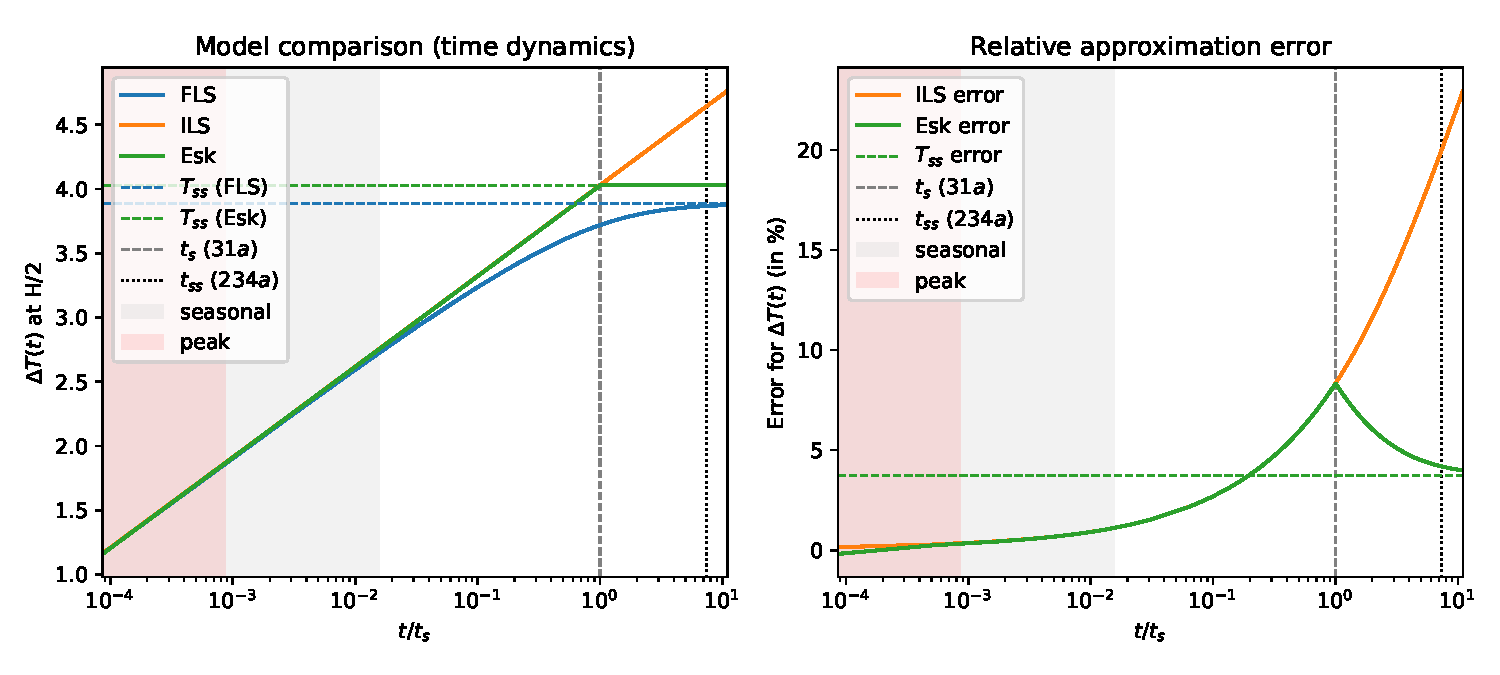
\includegraphics[width=.9\linewidth]{Figs/FLS_ILS_Esk_compare_ts.pdf}
    \caption{a) Temporal dynamics of the temperature variation along the borehole (shape of the "g-function") for the Finite Line Source (FLS), Infinite Line Source (ILS) and asymptotic (Esk) models, b) relative error for the temperature variation, as percentage of the $\Delta T_{FLS}$. The time duration of peak (red) and seasonal (grey) effects are highlighted.}
    \label{fig:T_dynamics}
\end{figure}
\end{comment}

\subsubsection{Approximations and errors}

The FLS can be simplified under certain assumptions by simpler models, namely the infinite line source model (ILS) and an asymptotic approximation of the FLS model, which are described in Appendix~\ref{app:allModels}.
% A comparison of all methods is provided in Section~\ref{comparison}.
These models, used in the literature for example in \cite{alcaraz_advection_2016,alcaraz_t-i-ger_2017,casasso_g.pot:_2016}, show a negligible deviation from the FLS model for time spans below 1 year (see Fig. \ref{fig:T_dynamics})b and are hence well-suited for modelling seasonal and peak effects (see Appendix~\ref{app:allModels} for details).
%
For larger time spans of several years, the deviation of the approximations from the FLS solution becomes non-negligible.
% While the ILS solution does not achieve a steady state due to its infinite length, the error of the Esk approximation peaks around the time constant $t/t_s=1$, leading to a maximum deviation of around 8\% and an error of around 4\% in the steady state (dashed line in Fig. \ref{fig:T_dynamics}b).
% As the dimensioning horizon typically lies in the order of magnitude of $t_s$ (34 years for a BHE of length 100 m), these deviations are accumulated to significant errors when spatial superposition is applied.
This leads to a significant accumulation of errors when superposition is applied.
Throughout this work, the FLS is hence used to model long-term thermal resistances, similar to other studies accounting for spatial superposition \cite{miglani_methodology_2018,rivera_increased_2017}.

\begin{comment}
\textbf{Infinite Line Source (ILS)}. The ILS approximation is defined as \citep{poppel_grenzabstande_2017}:

\begin{equation}
\label{eq:ILS}
    \mathrm{g}_{ILS}(r, t) = \frac{1}{2} \int_\frac{r^2}{4 \alpha t}^\infty \frac{e^{-u}}{u}du 
                  = \frac{1}{2} E_1\left(\frac{r^2}{4 \alpha t}\right)
\end{equation}

The error between the ILS and FLS is negligible for $t < 0.1 t_s$ \citep{claesson_conductive_1988}, making it particularly suitable for short and medium-term analyses. For $t<t_s$, it is accurate with a bounded error (see \ref{comparison}), but as it does not reach a steady state (due to the assumed infinite length), it is not suitable for modelling ground temperature at $t>t_s$.
\\

\textbf{Eskilson's approximation (Esk)}.
\citet{eskilson_thermal_1987} proposes to model the temperature drop along the borehole as a function of the two asymptotes of the FLS model. The lower asymptote is valid for $t < t_s$ and represents the transient behaviour ($\mathrm{g}_{Esk, trans}$). For $t > t_s$, the upper asymptote represents the (quasi) steady-state ($\mathrm{g}_{Esk, qss}$). The g-function of the asymptotic approximation is hence defined as:

\begin{equation}
    g_{Esk}(r, t) = \left\{
        \begin{matrix}
            \mathrm{g}_{Esk, trans} & t_{min} < t < t_s   \\ 
            \mathrm{g}_{Esk, qss}    & t > t_s           
        \end{matrix} 
\right.
\end{equation}

The \textit{transient asymptote} is an approximation of the ILS \citep{wagner_erdwarmesonden._2019}. Two equivalent formulations of $\mathrm{g}_{Esk, trans}$ exist. The first is derived from the mathematical approximation of the exponential integral $E_1$ in Eq.~\ref{eq:ILS}, while the second represents the physical process. The expressions are \citep{pahud_geothermal_2002}: 

\begin{equation}
\label{eq:Esk_trans}
    \mathrm{g}_{Esk, trans}(r, t) = \frac{1}{2} \left(\ln\left(\frac{4 \alpha t}{r^2}\right) - \gamma\right)
                                  = \ln\left(\frac{H}{2 r}\right) + \frac{1}{2} \ln\left(\frac{t}{t_s}\right), \quad
    t_{min} < t < t_s
\end{equation}

While the second expression is more intuitive, the first provides more information on the validity of the approach. It is derived from the following approximation of the exponential integral:

\begin{equation}
\label{eq:apx}
    E_1\left(x\right) \approx \ln\left(\frac{1}{x}\right) - \gamma, \quad x \ll 1
\end{equation}

where $\gamma$ is Euler's constant (0.57221...). To obtain Eq.~\ref{eq:Esk_trans}, we substitute Eq.~\ref{eq:apx} in Eq.~\ref{eq:ILS}.
Equation~\ref{eq:apx} approximates the ILS for all $x < 0.05$ with negligible error. For $x = r^2/(4 \alpha t)$ and $r = r_b$ (the borehole wall), this gives a minimum time for the transient asymptote of:

\begin{equation}
    t_{min} = \frac{5 r_b^2}{\alpha}, \quad r_b \ll H
\end{equation}

The values of $t_{min}$ typically lie below $6h$, so the condition is fulfilled for all timescales of interest.

If the temperature at larger distances from the borehole is of interest ($r \gg r_b$), for example for modelling borehole fields, the condition for the validity of Eq.~\ref{eq:Esk_trans} becomes:

\begin{equation}
\label{eq:r_cond}
    r < \sqrt{(0.2 \alpha t )}
\end{equation}

The interaction between boreholes is only of interest in the long term. On this temporal scale, we obtain $r_{dim} < 18m$ for the planning horizon of 50 years, $r_{qss} < 0.15H$ for $t_s$ and $r_{ss} < 0.4H$ for $t_{ss}$.

The \textit{steady-state asymptote} approximates the steady-state solution of the FLS (Eq.~\ref{eq:FLS_ss}). We refer to it as \textit{quasi steady-state}. According to \citet{eskilson_thermal_1987}, the quasi steady-state is given by:

\begin{equation}
\label{eq:Esk_qss}
    \mathrm{g}_{Esk, qss}(r) = \ln\left(\frac{H}{2 r}\right), \quad t > t_s
\end{equation}

From Eqs.~\ref{eq:Esk_trans} and \ref{eq:Esk_qss} it is easy to see that the two asymptotes intersect at $t = t_s$.
As the Esk model is practically equivalent to the ILS solution for $t_{min} < t < t_s$ (provided Eq.~\ref{eq:r_cond} is fulfilled), the transient asymptote has a negligible error with respect to the FLS for $t < 0.1 t_s$, and a bounded error for $t = t_s$. The transient asymptote also has a bounded error with respect to the FLS.

\subsubsection{Model comparison}
\label{comparison}

As mentioned above, the approximations of the FLS model are valid under certain assumptions, but may significantly speed-up the modelling time (even though the formulation in Eq.~\ref{eq:FLS_int} is already much faster than Eq.~\ref{eq:FLS}). To understand the ranges of validity and the error induced by the use of the approximations, we compare the different models for different time scales and distances to the borehole. All examples are shown for a borehole of 100m length, but the patterns are nearly identical for longer BHE's. In general, the temperature drop ($\Delta T$) along the borehole is smaller for larger $H$, hence leading to smaller absolute, but similar relative errors. 

Figure~\ref{fig:T_dynamics} shows a comparison between the models for different time scales at the borehole wall ($r = r_b$). We can see that for short time scales (red/grey), all models have a negligible error (up to $1\%$). 
Hence, any approximation may be used to model both peak and seasonal effects. At larger time scales, the ILS model starts to diverge from the FLS solution. 
This is expected, as the ILS never reaches a steady-state due to its infinite length. In this context, \citet{bandos_finite_2009} provide a formulation for a semi-infinite line source (SILS), which does reach a steady state. 

The Esk model is quasi-equivalent to the ILS for $t_{min} < t < t_s$, and reaches its steady-state for $t > t_s$. The figure shows that the upper asymptote overestimates the steady-state temperature by $3.7\%$, with the largest error occurring around $t = t_s$ ($\approx 8\%$). These percentages are valid for all borehole lengths. 
For typical boreholes of $H=100-200m$, the time scales with the maximum error (around $t_s$) correspond to the time scales of highest interest. 
As the absolute difference is relatively small, this may not have a large impact for modelling individual boreholes, and the asymptotic steady-state $\mathrm{g}_{Esk, qss}$ can be safely used. For modelling large borehole fields, however, the error accumulates, which can lead to significant differences in the estimated potential. For large-scale studies, the exact FLS solution should hence be used.

\begin{figure}[t]
    \centering
    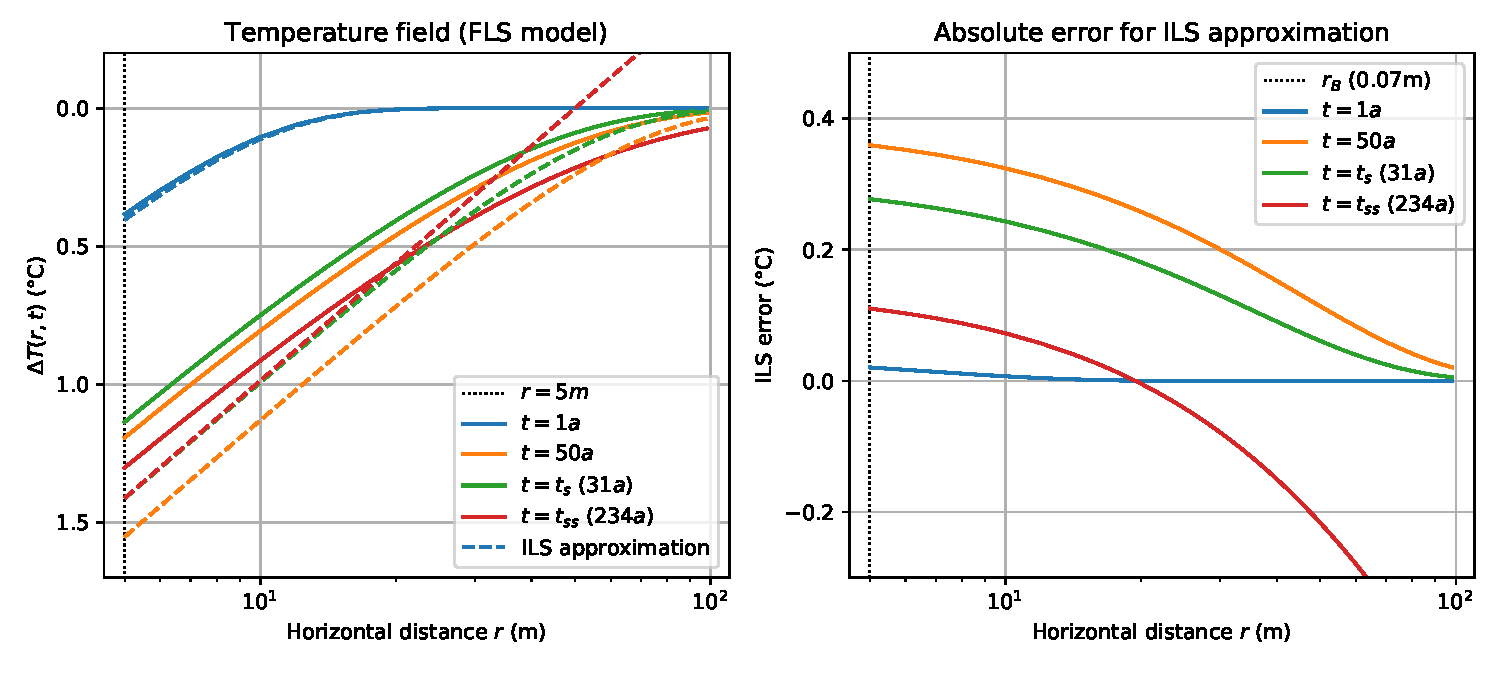
\includegraphics[width=.9\linewidth]{Figs/FLS_ILS_compare_r.pdf}
    \caption{a) Temperature field with distance to the BHE (length 100m) on logarithmic scale. The Infinite Line Source (with $\mathrm{g}_{Esk, qss}$ for $t = t_{ss}$) is shown for comparison (dashed lines). b) Absolute error (in $\circ$C) for the ILS model. The example shows a BHE of 100m length.}
    \label{fig:r_field}
\end{figure}

To assess the effect of adjacent boreholes, the temperature fields at large distances from the borehole ($5m < r < H$) are of interest. As seasonal and peak effects have a penetration depth that is lower than the minimum borehole distance of $5m$, only long-term effects are relevant. Figure~\ref{fig:r_field} shows the temperature drop in the ground for three long-term time intervals: the typical planning horizon ($t_{dim}$) for BHEs of 50 years, the quasi-steady-state $t_s$, where the temperature drop has reached around $95\%$ of its final value, and the actual steady state ($t_{ss}$). For comparison, also a short horizon of 1 year is shown.

While the temperature drop increases logarithmically for small distances, it trails off for distances that approach the borehole length $H$. In this range, Eq.~\ref{eq:apx} is no longer valid, so the transient asymptote cannot be used. This can be seen by the unrealistic steady-state solution, which represents the Esk steady-state asymptote (see Eq.~\ref{eq:Esk_qss}). It reaches a value of $0$ at $H/2$ and has negative values after, which is infeasible.

As Fig.~\ref{fig:T_dynamics} suggests, the error between the ILS and the FLS model increases with time, up to $0.1-0.3 ^\circ$C for the radii of interest. While this may  be negligible for a single neighbor, the error accumulates for borehole fields.  The exact FLS solution should hence be used for modelling large-scale geothermal potentials.
\end{comment}

\subsubsection{Long-term, seasonal and peak effects}
\label{seas_peak}

Based on the analytical models described above, mathematical formulations for the thermal resistance of the peak, seasonal and long-term components shown in Fig.~\ref{fig:q_seasonal} ($R_{LT},R_{seas},R_{peak}$) can be derived. 
% As it was shown in Fig.~\ref{fig:q_seasonal}, the minimum temperature at the borehole wall consists of a long-term, a seasonal and a peak component, each obtained by multiplying the respective heat extraction rate ($\overline{q}, q_{seas}, q_{peak}$) with its thermal resistance ($R_{LT},R_{seas},R_{peak}$, see Eq.~\ref{eq:dT_b}). 

\textbf{Long-term effects} are assessed at $t = t_{dim}$ using the FLS solution for an accurate model of the spatial superposition \cite{miglani_methodology_2018,rivera_increased_2017}.
% (typically 50 years), at quasi steady-state ($t = t_s$) or at steady state ($t = t_{ss}$). It is common to use the quasi steady-state asymptote for a conservative approximation of a \textit{single borehole}, as it overestimates the maximum temperature drop (see Fig.~\ref{fig:T_dynamics}). Examples for this approach are \cite{claesson_conductive_1988} and \cite{pahud_geothermal_2002}. 
%
Applying the principle of spatial superposition, 
% For \textbf{multiple boreholes}, the g-functions of each borehole are superposed. As we saw in Section \ref{comparison}, only the exact FLS is appropriate for a realistic superposition of multiple BHEs, as an accumulation of the error should be avoided.
the long-term resistance of borehole $i$ surrounded by $N$ boreholes may be expressed as (cf. \cite{claesson_analytical_2011}):

\begin{equation}
\label{eq:R_LT_superposed}
    R_{LT, i}(H) = \frac{1}{2 \pi \lambda} \mathrm{g}_{FLS}(r_b, H) + \frac{1}{2 \pi \lambda} \sum_{j=1}^N \mathrm{g}_{FLS}(r_{i,j}, H) 
\end{equation}
where $i \neq j$, $\mathrm{g}(r, H)$ is obtained from Eq.~\ref{eq:FLS_int} and $r_{i,j}$ denotes the distance between borehole $i$ and the surrounding borehole $j$. If a single borehole is considered, only the first term of the addition is relevant. To ease the notation, the argument $t = t_{dim}$ has been omitted from Eq.~\ref{eq:R_LT_superposed}.

\textbf{Seasonal effects} are modelled in this work as a periodic heat extraction. Effects from neighboring boreholes can be ignored if the minimum spacing ($B_{min}$) fulfills the following condition:

\begin{equation}
    B_{min} > 0.7 \sqrt{\alpha t_{seas}}
\end{equation}

As the minimum spacing is defined as 5 m in the SIA norm \cite{sia_sondes_2010}, this criterion is fulfilled for the period of the seasonal variation ($t_{seas} = 1$ year). The thermal diffusivities in Switzerland (see Table~\ref{tab:phys_params}) result in $B_{min} \approx 3.5-4.5$ m. The maximum periodic thermal resistance is given by \citep{claesson_conductive_1988, pahud_geothermal_2002}:

\begin{equation}
    R_{seas}(t_\mathit{seas}) = \frac{1}{2 \pi \lambda} \sqrt{\left(\ln(2/r_{pb}^\prime \right) - \gamma)^2 + \pi^2/16}
\end{equation}

where
\begin{equation*}
    r_{pb}^\prime = r_b \sqrt{2}/\delta < 0.1, \quad \delta = \sqrt{ \alpha t_\mathit{seas} / \pi}
\end{equation*}
The $R_{seas}$ is based on the ILS model, and hence it is independent of the borehole depth $H$.
The penetration depth of the temperature drop is denoted as $\delta$, which is around $3-4$ m for Switzerland. Seasonal effects hence do not impact adjacent boreholes. 

\textbf{Short-term effects} are represented by a heat extraction pulse at $q_{max}$ for a duration $t_\mathit{peak}$, typically 1-10 days (see Table~\ref{tab:tech_design_params}). Due to the short duration of the pulse, the ILS approximation is valid with negligible error (see Appendix \ref{app:allModels}). Thermal effects have an even smaller penetration depth than seasonal effects, so no surrounding boreholes need to be considered. The thermal resistance can hence be obtained as:

\begin{equation}
    \mathrm{R}_\mathit{peak}(t_\mathit{peak}) = \frac{1}{2 \pi \lambda} \ \mathrm{g}_{ILS}(r_b, t_\mathit{peak})
\end{equation}
where $\mathrm{g}_{ILS}$ is obtained from Appendix \ref{app:allModels}.
While peak effects are relevant when modelling the operation of GSHP systems \cite{miglani_methodology_2018}, they are frequently neglected in studies of the long-term technical geothermal potential, as a back-up heating system is available in most cases to cover peak extractions which may violate the temperature constraint (Eq.~\ref{eq:T_mf_min}). We follow this approach and neglect peak heat extraction throughout this work. 


%\section{Hybrid system optimization}

\cleardoublepage
\chapter{Machine Learning and \mbox{uncertainties}}
\label{methods_ML}

\vspace{-15pt} % one line spacing corresponds approx to 15 pts
\begin{tcolorbox}[enhanced,width=\textwidth,size=fbox,
        sharp corners,colframe=black!5!white,drop fuzzy shadow southeast,
        boxrule=3mm, parbox=false] 
        
This chapter borrows from the article \citep{walch_big_2020}:

\qquad \bibentry{walch_big_2020}

and the conference proceedings \cite{walch_spatio-temporal_2019, walch_fast_2019}:

\quad \bibentry{walch_spatio-temporal_2019} 

\quad \bibentry{walch_fast_2019}
\end{tcolorbox}

The large-scale estimation of HyREP at high spatial and temporal resolution challenges the analytical and geospatial models from Chapter~\ref{methods_physical}, for three main reasons.
First, some data required to perform the analytical and geospatial modelling may not be available across the entire region for which the HyREP is computed.
Second, the resolution or quality of some of the input datasets may be insufficient to assure a high-resolution potential estimation, but it could be improved through the use of additional information.
Third, these physics-based approaches may be too computationally intensive, inhibiting their application at the large scale.
The use of Machine Learning (ML) as a method to address the above limitations of "classical" physics-based models has attracted increasing attention in recent years \cite{willard_integrating_2020}. 

In this thesis, we use ML to address several of the above-mentioned limitations for the national-scale estimation of RPV (Chapter~\ref{solar}) and GSHP (Chaper~\ref{geothermal}) potential. 
The ML models hereby % To this aim, ML is used in two contexts: 
% (i) To 
learn and predict the relationship between a set of input data (\textit{features}) and output variables (\textit{targets}), known as \textit{supervised learning}, 
% and (ii) to group data based on similarities in its features and to identify outliers, known as \textit{clustering}. 
as summarized in Section~\ref{ML_supervised}.
For an in-depth introduction to Machine Learning, interested readers may refer for example to \citet{bishop_pattern_2006}.
\nomenclature[A]{ML}{Machine Learning}

The use of data-driven methods further requires the estimation of \textit{uncertainties} related to the ML predictions, which are essential for decision-making processes \cite{knusel_argument-based_2020}. 
Uncertainties may arise for example from noise in input data sources or from the modelling approaches themselves, and their quantification is a vast field of research \cite{willard_integrating_2020,knusel_argument-based_2020}.
We model uncertainties arising from data noise and from ML models in the form of standard deviations, which we propagate through the analytical models presented in Chapter~\ref{methods_physical}. 
% The following sections will provide an overview of the supervised learning  and clustering techniques used in this thesis, as well as 
Section~\ref{unc} provides an overview of the applied methods for a systematic quantification of uncertainties through combined physics-based and data-driven modelling approaches. 

\section{Supervised learning}
\label{ML_supervised}

Supervised learning algorithms are trained on a set of input features and corresponding output targets, such as to minimise the error between an algorithm's prediction and the "true" target.
Several design choices can influence the performance of supervised learning algorithms: (i) the choice of the input features, (ii) the choice of an appropriate ML model for a given problem, and (iii) the
choice of the parameters defining the model structure (hyper-parameters).
The selection of suitable input features varies largely between different ML applications and is often based on expert knowledge. 
The full set of available features, obtained using expert knowledge or otherwise, may however contain features which are redundant or even detrimental to the ML model's performance.
Feature exploration and selection techniques may hence be used to enhance the quality of the feature set (Section~\ref{ML_features}).

The choice of an appropriate ML model depends on the structure of the problem and the available data. Regression algorithms are used to model continuous targets, while classification algorithms are used for binary or multi-class targets (see Section~\ref{ML_models}). Furthermore, some algorithms such as Support Vector Machines (SVM) may be better suited for high-dimensional feature sets (i.e. many features), while other algorithms such as Extreme Learning Machines (ELM) are optimized for very large datasets. For image or natural language processing, convolutional neural networks (CNNs) have gained high popularity in recent years.
% For many applications, however, multiple algorithms may be appropriate and their performance should be compared to choose the best model.

For any ML model, the optimization of its hyper-parameters is performed during the so-called \textit{tuning} procedure in the training phase. For model training, the labelled data (all data samples for which both features and targets are known) are divided into three random subsets: 
(i) The \textit{training} set, which is used to fit the model, (ii) the \textit{validation} set, which is used to assess the performance during model tuning, and (iii) the \textit{test} set, which is excluded from the tuning procedure and used for the final model evaluation.
The test set usually contains $20 - 33\%$ of the labelled data. The remaining data is then split again, keeping another $20 - 33\%$ for model validation.
To reduce the randomness in the splitting of the data into training and validation sets, a $k$-fold cross-validation (CV) procedure is widely applied in the literature. 
For this, the training data is randomly split into $k$ subsets (folds), from which $k$ ML models are trained. Each model uses ($k$ – 1) folds for training and the last fold for validation. 
Unless mentioned otherwise, we use a 5-fold cross-validation ($k$ = 5) throughout this work.
% 
% Often regarded as black-box models, ML algorithms are trained based on a set of input data (called features), such as to predi ct an output (the target or label). 
% The architecture of each model is determined through a tuning procedure in the training phase, where the parameters defining the model structure (hyper-parameters) are optimized in order to minimize the difference between the prediction and the target. 

\subsection{Feature exploration and selection techniques}
\label{ML_features}

A vast variety of methods exist in the literature for the exploration, analysis and selection of appropriate features for ML models, which are often highly dependent on the application. In this section we introduce five concepts for designing ML feature sets which have proven useful for the ML applications presented in this thesis.

\textbf{Correlation analysis} provides insights into potential redundancies between different features, and allows to obtain a first quantitative measure of the relevance of each feature towards predicting the target variable(s).
In addition to the widely used Pearson correlation coefficient, which measures linear correlations, other measures of non-linear dependencies between variables may be used, such as Spearman's rank correlation coefficient \cite{kokoska_crc_1999} or mutual information \cite{kozachenko_statistical_1987}. While low correlations are desirable between the different features, indicating low redundancy within the feature set, high correlations between the features and the target suggest a high importance towards predicting this target.

\textbf{Feature transformation} includes the normalisation of the features, typically to zero mean and unit variance, but it may further refer to non-linear transformations of the features or the target. While normalisation is standard practice and required for many ML algorithms, the suitability of non-linear transformations depends on the data. For example, log-transformations may significantly improve the predictions for features at exponential scale. Feature visualisation through histograms or scatterplots can provide insights into suitable transformations.

\textbf{Principal Component Analysis (PCA)} \cite{tipping_probabilistic_1999} is an advanced feature transformation technique which yields a set of independent (principal) components. These components are ranked according to the percentage of explained variance in each component. To select features using PCA, the minimum percentage of explained variance may be defined, such that the last-ranked components up to the required percentage of explained variance are discarded. 
The advantage of this method is that it yields only independent components, which is favourable for the performance of many ML models, and it can drastically reduce the number of features in high-dimensional problems. However, the PCA is based on the features only and contains no information on the relevance of the features to predicting the target. It further requires all available features as input, so it cannot be used to reduce the number of input variables.

\textbf{Sequential backward selection (SBS) }\cite{ferri_comparative_1994} is one method that can be applied to reduce the number of features. Its advantage is that it can be applied to any ML algorithm, using any metric of evaluation. 
Starting from the complete feature set, the SBS iteratively excludes one feature at a time and computes the error for the prediction using the reduced feature set. The feature whose exclusion causes the lowest change in prediction error ($\Delta_{err}$) is permanently removed from the set of features. This procedure is repeated until only one feature remains, and the $\Delta_{err}$ is recorded for each iteration.
To reduce the number of features, a threshold for $\Delta_{err}$ can be applied, selecting all features that keep $\Delta_{err}$ below the threshold.
% is chosen, which represents the maximum tolerable increase in prediction error. The selected features are those which form the smallest feature set that keeps $\Delta_{err}$ below its threshold. 
As the number of iterations increases with the number of features, this procedure may not be applicable for high-dimensional problems.
%
In this work, feature selection is performed using the k-Nearest Neighbour algorithm (see Section~\ref{ML_models}) due to its fast computational time, and using the mean-squared error (MSE, Table~\ref{tab:error_metrics}) as performance metric in a 5-fold CV (see above).
% Any metric eor the selection is the mean-squared error (MSE) between the target (annual $G_t$) and the predicted value, which is obtained using 5-fold CV (see above). 

\textbf{Feature importance.} In addition to the above methods, which provide some insights into the importance of the features towards predicting the target, some ML algorithms provide a measure of feature importance as part of their algorithm's design.
Notably, decision tree algorithms (e.g. Random Forests) provide such a measure of feature importance. As the dataset is split at each node of the decision tree (see~\ref{fig:rf}) based on a threshold for one feature, the reduction of the impurity (or variance) in the targets due to each feature can be quantified \cite{breiman_random_2001}.
As redundancy between features may lead to misleading importance scores, this measure of feature importance should be combined with other analysis techniques.

\subsection{Regression and classification models}
\label{ML_models}
\label{RF}

\subsubsection{Regression}

\begin{table}[b]
\footnotesize
\centering
\caption{Error metrics in regression problems for a data set of $n$ samples, where $y_i$ is the target, $\hat{y}_i$ is the predicted value for sample $i$, $\bar{y}$ is the mean of $y_i$ and $\epsilon$ is a small positive number to avoid undefined MAPEs.} %  ($\bar{y}=\frac{1}{n} \sum_{i=0}^{n-1} y_{i}$)
\label{tab:error_metrics}
% \resizebox{\textwidth}{!}{%
\begin{tabular}{lcl}
\hline
\textbf{Metric} & & \textbf{Definition} \\ \hline
&&\\[-2ex]
\textit{R$^2$} &=& $\displaystyle 1-\frac{\sum_{i=0}^{n-1}\left(y_{i}-\hat{y}_{i}\right)^{2}}{\sum_{i=0}^{n-1}\left(y_{i}-\bar{y}\right)^{2}}$ \\[3ex]
\textit{MSE} &=& $\displaystyle \frac{1}{n} \sum_{i=0}^{n-1}\left( y_i - \hat{y}_i \right)^2$ \\[3ex]
\textit{RMSE} &=& $\displaystyle \left(\frac{1}{n} \sum_{i=0}^{n-1}\left( y_i - \hat{y}_i \right)^2\right)^{1/2}$ \\[3ex]
\textit{MAE} &=& $\displaystyle \frac{1}{n} \sum_{i=0}^{n-1}\left| y_i - \hat{y}_i \right| $ \\[3ex]
\textit{MAPE} &=& $\displaystyle \frac{1}{n} \sum_{i=0}^{n-1} \frac{\left| y_i - \hat{y}_i \right|}{\max(\epsilon,y_i)}$ \\[3ex]
\textit{MBE} &=& $\displaystyle \frac{1}{n} \sum_{i=0}^{n-1}\left( y_i - \hat{y}_i \right) $\\[3ex]
\textit{logMSE} &=& $\displaystyle \frac{1}{n} \sum_{i=0}^{n-1}\left( \log(1 + y_i) - \log(1 + \hat{y}_i) \right)^2$ \\[2ex] \hline
\end{tabular}
% }
\end{table}

Regression algorithms are used to predict continuous variables, such as solar radiation or shallow geothermal heat. 
During model training, the (internal) parameters of the regression algorithms are optimized such as to minimise the error between the continous targets and the predictions of the model.
This error (also referred to as the loss function) is typically defined as the mean squared error (MSE), i.e. the mean of the squared difference between the predictions and the "true" targets.
%
For model tuning and performance evaluations, further error metrics are widely used (see Table~\ref{tab:error_metrics}).
These include (i) the R$^2$-coefficient of determination, indicating the goodness of fit between predictions and targets, (ii) the root-mean-squared error (RMSE), which has the same unit as the target, (iii) the mean average error (MAE), (iv) the mean average percentage error (MAPE), (v) the mean bias error (MBE), and (vi) the mean squared logarithmic error (logMSE), which is useful for targets with an exponential growth \cite{pedregosa_scikit-learn:_2011}.


\subsubsection{Classification}
Classification algorithms are used for predicting discrete targets, either in a binary format (0 or 1) or as multiple classes, for example to differentiate between roof shapes \cite{mohajeri_city-scale_2018}.
The discrete nature of the targets requires different metrics to assess the prediction results. 
In classification tasks, the loss-functions used in the training procedure are either cross-entropy, also known as negative log-loss \cite{bishop_pattern_2006}, or the gini impurity \cite{breiman_classification_1984}. Both measures are designed to maximise the likelihood of a correct classification result, whereby the gini impurity is primarily used in classification trees.

For model tuning and performance evaluation, the number of correct and incorrect predictions is evaluated and displayed in a so-called confusion matrix, shown in Table~\ref{tab:conf_matrix} for the case of binary classification. From this confusion matrix, several evaluation scores can be derived. These include (i) the overall accuracy (OA), namely the total number of correct classifications over the total number of samples, (ii) the precision, namely the correct predictions over the total predictions of a given class, (iii) the recall, i.e. the correct predictions over all true labels in a given class, and (iv) the f1-score, which is the weighted average of precision and recall ($2*\text{\textit{precision}}*\text{\textit{recall}}/(\text{\textit{precision}}+\text{\textit{recall}})$).
Assessing the ensemble of these error metrics is particularly relevant for cases of imbalanced classification, where the number of samples in one class is very small compared to the other class. 
%In these cases the OA may be close to 1, which is very misleading if the 
 
\begin{table}[tb]
\footnotesize
\centering
\caption{Structure of confusion matrix for binary classification and evaluation metrics derived from the confusion matrix, namely precision, recall and accuracy (italic font), with $\sum = TN+TP+FN+FP$.}
\label{tab:conf_matrix}
\begin{tabular}{llccc}
\hline
 &  & \multicolumn{2}{c}{\textbf{Predicted class}} & \multirow{2}{*}{\textit{\textbf{Recall}}} \\
 &  & \textbf{0} & \textbf{1} &  \\ \hline
\multirow{2}{*}{\textbf{True class}} & \textbf{0} & True negatives (TN) & False positives (FP) & $TN/(TN + FP)$ \\
 & \textbf{1} & False negatives (FN) & True positives (TP) & $TP/(TP + FN)$ \\ \hline
\textit{\textbf{Precision}} & \textit{} & $TN/(TN + FN)$ & $TP/(TP + FP)$ & \textit{\textbf{OA} $= TP+TN/\sum$} \\ \hline
\end{tabular}
\end{table}

\subsubsection{ML model architectures}

Throughout this work, we use and compare the performance of six supervised ML models from different families of algorithms: (i) Linear Regression (LIN), (ii) K-Nearest Neighbors (KNN), (iii) Support Vector Machines (SVM), (iv) Random Forests (RF), Artificial Neural Networks (ANN), and (iv) Extreme Learning Machine Ensembles (ELM-E). The description of the algorithms provided below focuses on regression problems, which dominate in the use of ML throughout this thesis. All algorithms can however be equally applied to classification problems. The architecture of the six considered algorithms is shown in Fig. \ref{fig:ml_algorithms}.
\nomenclature[A]{LIN}{Linear Regression}
\nomenclature[A]{KNN}{K-Nearest Neighbours}
\nomenclature[A]{SVM}{Support Vector Machine}
\nomenclature[A]{RF}{Random Forest}
\nomenclature[A]{ANN}{Artificial Neural Network}
\nomenclature[A]{ELM}{Extreme Learning Machine}
\nomenclature[A]{ELM-E}{ELM Ensemble}


\begin{figure}[tb] % !
\centering
\makebox[\linewidth][c]{
\begin{subfigure}[t]{.3\textwidth}
  \centering
  \fbox{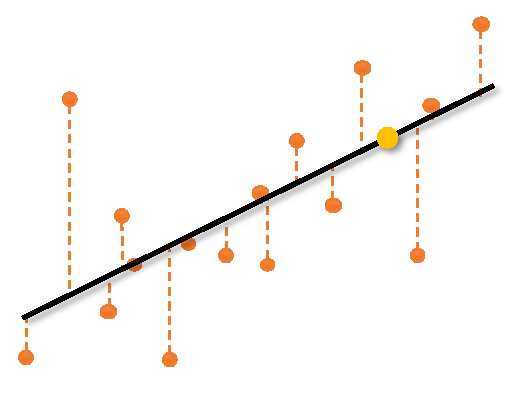
\includegraphics[width=.9\linewidth]{images/Figs/lin.pdf} } 
  \subcaption{\textbf{LIN}}
  \label{fig:lin}
\end{subfigure}
\begin{subfigure}[t]{.35\textwidth}
  \centering
  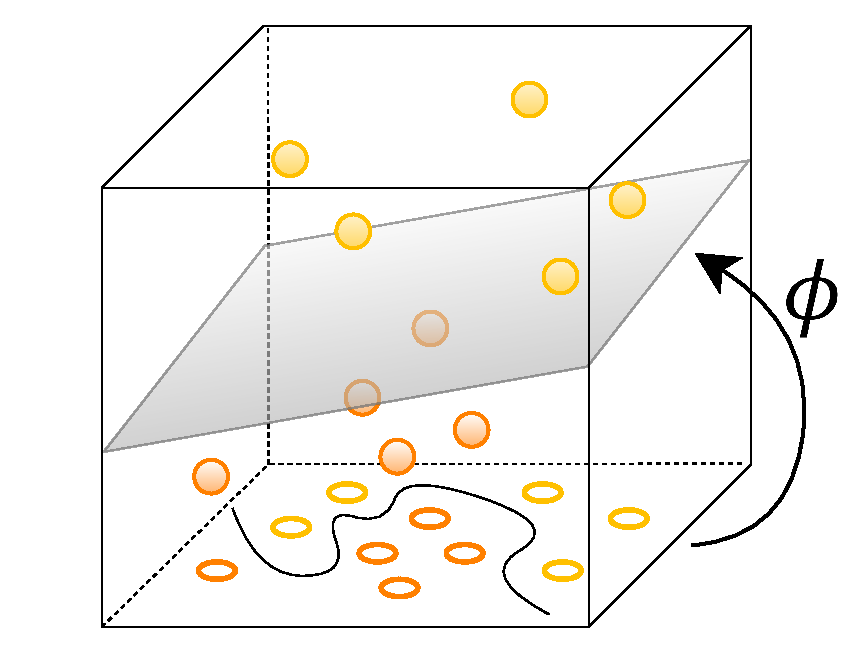
\includegraphics[width=.9\linewidth]{images/Figs/SVM.pdf} 
  \subcaption{\textbf{SVM}}
  \label{fig:svm}
\end{subfigure}
\begin{subfigure}[t]{.35\textwidth}
  \centering
  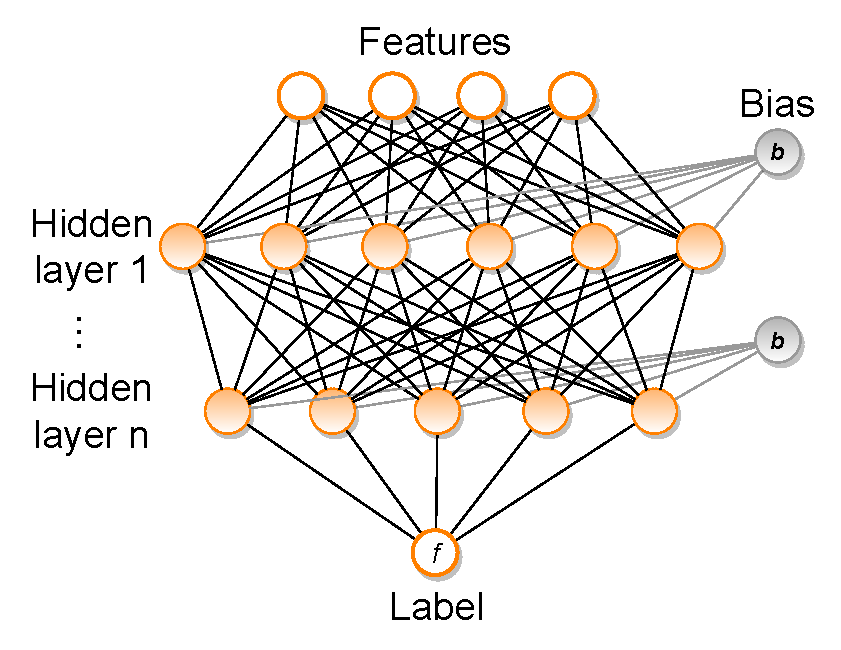
\includegraphics[width=.95\linewidth]{images/Figs/ANN.pdf}
  \subcaption{\textbf{ANN}}
  \label{fig:ann}
\end{subfigure}
} \\ \vspace{.25cm}
\makebox[\linewidth][c]{
\begin{subfigure}[t]{.3\textwidth}
  \centering
  \fbox{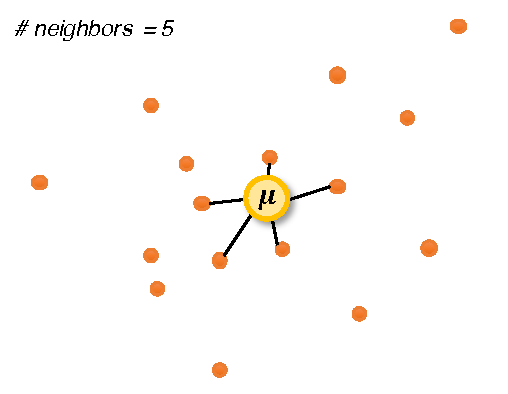
\includegraphics[width=.9\linewidth]{images/Figs/knn.pdf} }
  \subcaption{\textbf{KNN}}
  \label{fig:knn}
\end{subfigure}
\begin{subfigure}[t]{.35\textwidth}
  \centering
  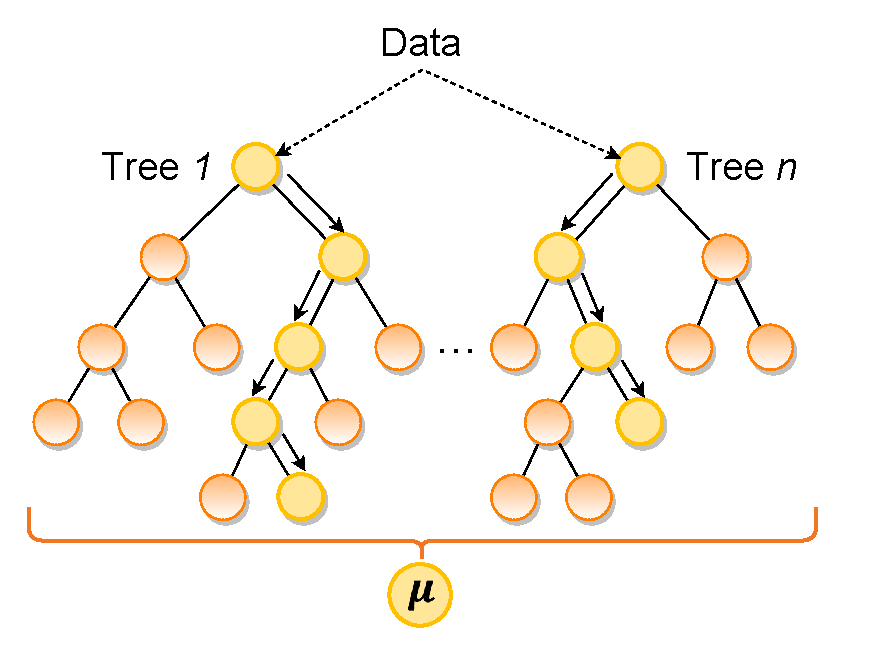
\includegraphics[width=.95\linewidth]{images/Figs/RF.pdf}
  \subcaption{\textbf{RF}}
  \label{fig:rf}
\end{subfigure}
\begin{subfigure}[t]{.35\textwidth}
  \centering
  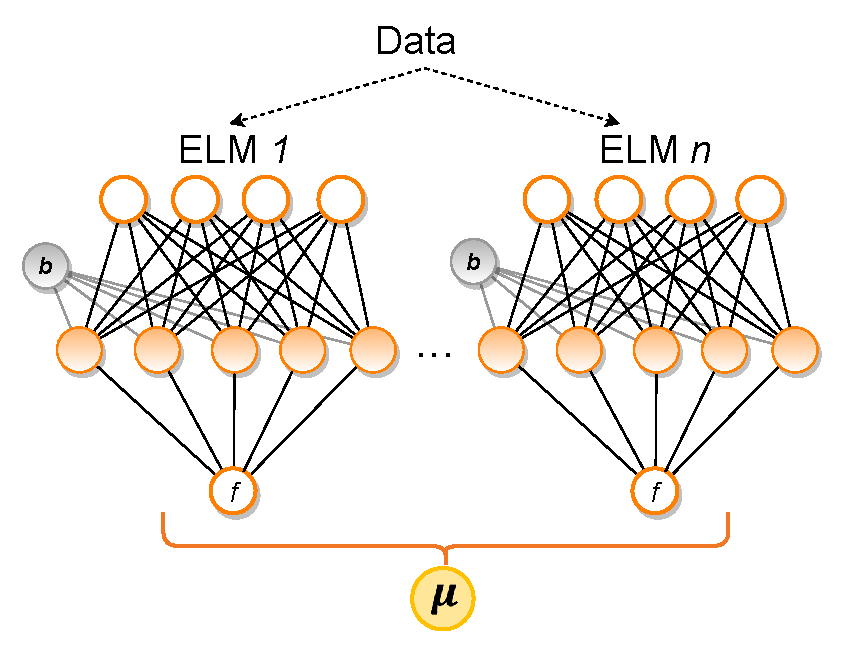
\includegraphics[width=.95\linewidth]{images/Figs/ELM_E.pdf}
  \subcaption{\textbf{ELM-E}}
  \label{fig:elme}
\end{subfigure}
}
\caption{Visualisation of ML algorithms used in this work. The selected algorithms are (a) Linear regression (LIN), (b) K-Nearest Neighbor Regression (KNN), (c) Support Vector Machine (SVM), (d) Random Forest (RF), (e) Artificial Neural Network (ANN), (f) Extreme Learning Machine Ensemble (ELM-E).}
\label{fig:ml_algorithms}
\end{figure}

\textbf{Linear Regression }(Fig. \ref{fig:lin}) assumes that the target is a linear function of the inputs. The prediction is obtained from the linear combination of the features which minimizes the residual sum of squares between the target and predicted values. It is fast and requires no tuning of hyper-parameters but shows a low accuracy for non-linear problems. The equivalent classification apporach for the linear regression is logistic regression, which estimates the probability of a data sample to belong to a specific class.

\textbf{K-nearest Neighbor Regression} (Fig. \ref{fig:knn}) is an interpolation algorithm, which computes a prediction as the average of the targets of the $k$ training samples whose features are closest to the given inputs. In classification, the average is replaced by a "majority voting" of the $k$ neighbours. The training dataset works as a look-up table for the predictions, which makes it effective for low-dimensional problems but inefficient for large datasets. We use the Euclidean distance as a measure of “closeness” and tune the number of neighbors ($k$).

\textbf{Support Vector Machine} (Fig. \ref{fig:svm}), introduced by \citet{cortes_support-vector_1995}, is the most popular algorithm in the family of kernel methods. It exploits the \textit{kernel trick}, which projects the features to a higher-dimensional space that allows for linear modelling. Its structure makes it particularly effective for high-dimensional problems, but it does not scale well with the number of samples. In this work, we use $\varepsilon$-Support Vector Regression with a radial basis function as kernel and tune the kernel coefficient ($\gamma$), the penalty parameter (C) and the error tolerance ($\varepsilon$).

\textbf{Random Forest} (Fig. \ref{fig:rf}) is an ensemble (i.e. an aggregation) of decision trees, which was proposed by \citet{breiman_random_2001}. Each of the decision trees in the ensemble pass a training sample along a set of nodes based on a threshold (defined during training) until a leaf node is reached. The prediction of each tree is obtained by averaging (or majority voting) the target values in the respective leaves. It is a popular algorithm due to its good predictive power and high robustness. Its main hyper-parameters are the number of features considered for the optimization of each threshold ($m_{ftrs}$), the minimum number of samples in each leaf ($m_{leaf}$) and the number of trees in the ensemble ($n_{est}$).
% A COMMENT ON FEATURE IMPORTANCE

\textbf{Artificial Neural Networks} (Fig. \ref{fig:ann}) consist of multiple layers of neurons, which are connected to the previous and the next layer through edges \cite{rumelhart_learning_1986}. From the input layer, which contains one neuron for each input, the data samples are passed through one or more hidden layers to the output layer with one neuron for each output. Each neuron computes a weighted linear combination of all nodes of the previous layer (for fully connected networks), which is then passed through a non-linear activation function. The weights within the network are optimised using a backpropagation procedure \cite{lecun_efficient_2012}. The hyperparameters of the ANN include the network architecture, namely the number of hidden layers and the number of neurons in each layer, the selected nonlinear activation function and a regularisation term.  

\textbf{Extreme Learning Machine Ensemble }(Fig. \ref{fig:elme}) is a collection of single-layer neural networks (ELMs), which were developed by \citet{huang_extreme_2006}. Each ELM consists of a single hidden layer, which is trained a more efficient way than traditional neural networks (see above) by a single-step optimization using a least-squares approach, which avoids the need for back-propagation. This results in a faster training time and a low number of hyper-parameters. The aggregation of $n$ ELMs in an ensemble further increases the robustness of the model and reduces the risk of overfitting \cite{huang_trends_2015}. 
It further enables the estimation of uncertainties, as described in Section~\ref{unc_ML}.

To train the ELM ensemble, we apply a bootstrap-aggregating (bagging) approach \cite{breiman_bagging_1996} where each ensemble member is trained on one bootstrapped resample of the training data. Each bootstrap replicate is obtained by resampling the $N$ training samples $N$ times uniformly and with replacement. At the output, the predictions of each ELM are averaged to give the final estimation.
The main hyper-parameters to tune in the ELM-E are the size of the hidden layer ($m_{ELM}$) and the number of ELMs in the ensemble ($n_{ELM}$). Throughout this work, we use a sigmoid activation function, which is a common choice for regression problems \cite{huang_trends_2015}.

We use the ML implementations of the \texttt{scikit-learn} library for python \cite{pedregosa_scikit-learn:_2011} for all models except the ELM-E. As no functional open-source code for the ELM-E was available when this work was carried out, we have implemented the ELM-E ourselves (regression only) using the ELM model of the \textit{HPELM} package for python \cite{akusok_high-performance_2015}, which supports computational acceleration on graphical processing units (GPUs). 
\nomenclature[A]{GPU}{Graphical Processing Units}


% A SUBSECTION ON ENSEMBLES, OR SIMPLY TWO PARAGRAPHS

\begin{comment}
% SOURCE: ICAE conference paper
Extreme Learning Machines, as proposed by Huang et al. [11], are single-layer feed-forward neural networks which are trained using a single-step optimization. The training process of ELM is up to hundreds of times faster than the training of other machine learning algorithms [11]. For our model we aggregate \textit{M} ELM to an ensemble, as shown in Fig. 1. This is known to improve the generalization performance by reducing the risk of overfitting [6,9,12], and allows to estimate the uncertainty as described in Section 2.2. At the hidden layer of each ELM, the training points $x_i$ of dimensionality d are multiplied by the randomly chosen input weights w and added to the random bias b. An activation function ƒ( ) is applied to the resulting random projections for modelling nonlinear behaviour of the data. We use a sigmoid activation function in this study, which is a common choice for regression problems [12]. The hidden layer is multiplied by the output weights $\beta$ and summed to give the model output $\hat{y}i$ (see Eq.1). During training, only $\beta$ needs to be optimized.

For ensemble training, we apply a bootstrap-aggregating (bagging) approach [13] where each ensemble member is trained on one bootstrapped resample of the training data. Each bootstrap replicate is obtained by resampling the N training samples N times uniformly and with replacement. On average, every replicate contains 63.2\% of the original data, with some duplicated samples. At the output, the predictions $\hat{y}_\mathrm{i}^\mathrm{m}$ of each ELM are averaged to give the final estimation $\hat{y}_i$ as shown in Eq. 2. The generation of M bootstrap replicates comes at a computational cost. For the implementation of each ELM, we therefore use the python toolbox \textit{hpelm} with GPU acceleration [14]. This showed significant speed-up in performance compared to the standard CPU implementation. This implementation allows us to train and to test ELM ensembles with a large number of hidden neurons on our large environmental dataset.

\begin{equation}
\label{eq:elm}
\hat{y}_{i}^{m}=\sum_{j=1}^{L} \beta_{j}^{m} f\left(\mathbf{w}_{j}^{m} \mathbf{x}_{i}+b_{j}^{m}\right), \quad \mathbf{x}_{i} \in \mathbb{R}^{d}, \mathbf{w}^{m} \in \mathbb{R}^{L \times d}, \quad i=1, \ldots, N, \quad m=1, \ldots, M
\end{equation}

\begin{equation}
\label{eq:elm_mean}
\hat{y}_{i}=\frac{1}{M} \sum_{m=1}^{M} \hat{y}_{i}^{m}, \quad i=1, \ldots, N
\end{equation}

\section{Clustering}
\textbf{K-means clustering.}

\textbf{Density-Based Spatial Clustering of Applications with Noise (DBSCAN).}
\end{comment}


\section{Uncertainties}
\subsection{Uncertainty estimation for ensemble models}
\label{unc_ML}

% SOURCE: Initial submission PV paper
The ensemble structure of both ML ensemble algorithms used in this work (RF and ELM-E) permits the estimation of uncertainties arising from the modelling process (model uncertainty, $\hat{\sigma}_M$). The remaining residuals after the subtraction of the model variance are further used to estimate the uncertainty related to the data noise (data uncertainty, $\hat{\sigma}_D$) \cite{akusok_per-sample_2019,guignard_uncertainty_2020}. 
% This approach enables a specific characterization of the uncertainty for each spatio-temporal point.
It has been previously used to estimate for example wind speeds for wind power generation~\cite{wan_probabilistic_2014}.

The ensemble method is based on a bagging (bootstrap-aggregating) approach, which introduces randomness into the model  \cite{breiman_bagging_1996}.
Every ensemble member is trained on one bootstrapped resample of the training data, which is
obtained by sampling the training set uniformly and with replacement.
On average, every such resample contains 63.2\% of the original data, with some duplicated samples \cite{breiman_bagging_1996}. 
The model uncertainty is quantified as the standard deviation of the predictions of all model in the ensemble, which is computed as \cite{heskes_practical_1997}:

\begin{equation}
\label{eq:model_unc}
  \hat{\sigma}_M^2 (\mathbf{x}_i) = \frac{1}{N} \sum_{n=1}^N (\hat{y}_i^n - \hat{y}_i)^2, \quad i=1,...,L
\end{equation}

where $\hat{\sigma}_M$ denotes the model standard deviation, referred to as model uncertainty, $N$ denotes the ensemble length, $\hat{y}_i$ is the ensemble prediction for sample $\mathbf{x}_i$ and $\hat{y}_i^n$ is the prediction of ensemble member $n$.

Additionally to the model variance, we estimate the variance of the data noise by modelling the remaining residuals. They are derived by subtracting the model variance from the squared difference between $\hat{y}_i$ and the targets $t_i$, as shown below.
In order to reduce bias, the out-of-bag (OOB) model output are used, which is the mean of the ensemble members for which a given training data point was not considered (due to bootstrapping) \cite{heskes_practical_1997}. 

\begin{equation}
\label{eq:data_unc}
  \hat{\sigma}_D^2 (\mathbf{x}_i) = \max \left\{ (t_i - \hat{y}_i)^2 - \hat{\sigma}_M^2 (\mathbf{x}_i) , 0 \right\}, \quad i=1,...,L
\end{equation}
 
 where $\hat{\sigma}_D$ denotes the standard deviation of data noise, referred to as data uncertainty, and $t_i$ is the target value for sample $\mathbf{x}_i$. 
$\hat{\sigma}_D$ can only be computed if $t_i$ is known. Thus, a second ML model is trained from the residuals to predict $\hat{\sigma}_D$ for points with unknown targets. Unless mentioned otherwise, the same hyper-parameters are used in both models.

The total variance of a variable that is estimated using a ML model is the squared sum of its model uncertainty and its data uncertainty: 

\begin{equation}
\label{eq:total_unc}
\sigma^2 (\mathbf{x}_i) = \hat{\sigma}_M^2 (\mathbf{x}_i) + \hat{\sigma}_D^2 (\mathbf{x}_i), \quad i=1,...,L
\end{equation}

% Source: ICAE paper
% Applying bagging to the ELM ensemble increases the quality of the prediction and it also allows to compute the model uncertainty $\hat{\sigma}M$, derived from the variance ${\hat{\sigma}}_M^2$ of the M model outputs ${\hat{y}}_\mathrm{i}^\mathrm{m}$ (see Eq. 3) [9,15]. Afterwards, remaining residuals are derived by subtracting the model variance from the squared difference between the model outputs and the targets ti, as visible in Eq. 4. We compute these residuals for the training data, which are used to train a second ELM ensemble. The output is the data noise variance ${\hat{\sigma}}_D^2$, and the standard deviation $\hat{\sigma}D$ quantifies the data uncertainty. Adding model and data noise variance provides a qualitative estimate of the uncertainty on the predictions.

\begin{comment}
\subsubsection{Uncertainty for GIS methods}

The uncertainty for the GIS-derived and bias corrected quantities, namely $S_{sh}$ and $SVF$, is estimated from the residuals between the values computed using the $(2 \times 2)m^2$ and the $(0.5 \times 0.5)m^2$ resolution DSM in Geneva. The latter is considered the "true" surface model. 
The error in the GIS-derived quantities is treated as a random variable, whose first and second moments are estimated from the mean and the variance of the discrepancy. The mean is used for the bias correction, as explained in Sections \ref{shade} and \ref{svf}, while the variance represents the uncertainty.

It should be noted that the error of the GIS methods for $C_{sh}$ and $C_{pv}$ are not computed in the way described here, as they form part of the data uncertainty estimated by the subsequent ML models.
\end{comment}

\subsection{Uncertainty propagation}
\label{method_unc_prop}

For the estimation of renewable resource potential, different sources of uncertainties must be combined and propagated through physicals models. 
For this propagation of uncertainties, the correlation among the random variables plays a key role.
%
% SOURCE: Initial submission PV paper
% The correlation among the random variables plays a key role in the propagation of uncertainty. 
If statistical independence can be assumed, the mean and variance of the resulting variables can be computed from the mean and variance of each parameter only, which greatly simplifies the uncertainty propagation.
However, this assumption does not always hold, in which case correlations between random variables must be taken into account.
% As the uncertainty is computed separately for each spatio-temporal data point, we assume statistical independence between meteorological and building related parameters, namely between $G_h, G_B, G_D$ and $S_{sh}, SVF, A_{PV}$. This is valid as the uncertainty of the horizontal radiation is dominated by the meteorological conditions, while those of $S_{sh}(t), SVF, A_{PV}$ are related to the GIS and ML methods. These are independent and uncorrelated processes.
In the context of this thesis, we consider the propagation of uncertainties over a set of sums and products of random variables using error propagation theory \cite{jcgm_evaluation_2008, goodman_variance_1962}. This section summarises the error propagation formulas for summations and multiplications, applied in the following chapters, in their general form.

% In error propagation theory~\cite{jcgm_evaluation_2008, goodman_variance_1962}, the uncertainty on any final measurand is the result of the propagation over a set of sums and products of its variables. 
In error analysis, the variance of the sum of $N$ randomly distributed variables $X_i$ is given by:

\begin{equation}
\label{eq:unc_sum}
\mathrm{Var}\left(\sum_{i=1}^N X_i\right) = \sum_{i=1}^N\mathrm{Var}(X_i) + 2\sum_{i < j}\mathrm{Cov}(X_i, X_j)
\end{equation}
which simplifies to the sum of the variances of $X_i$ if the random variables are statistically independent.
%
The variance of the product of two random variables $X$ and $Y$ is defined as:

\begin{align}
\label{eq:var_mult_corr}
\mathrm{Var}(X Y)&=E\left(X^{2} Y^{2}\right)-E(X Y)^{2} \\
&= \mathrm{Cov}\left(X^{2}, Y^{2}\right)+\left[\mathrm{Var}(X)+\mathrm{E}(X)^{2}\right] \left[\mathrm{Var}(Y)+\mathrm{E}(Y)^{2}\right]-[\mathrm{Cov}\left(X, Y\right)+\mathrm{E}(X)  \mathrm{E}(Y)]^{2} \nonumber
\end{align}

If statistical independence between the random variables $X$ and $Y$can be assumed, the terms $\mathrm{Cov}\left(X^{2}, Y^{2}\right)$and $\mathrm{Cov}\left(X, Y\right)$ can be omitted, such that Eq.~\ref{eq:var_mult_corr} becomes a function of the variances of $X$ and $Y$ and their expected value:
\begin{equation}
\label{eq:unc_prod}
\mathrm{Var}(XY) = \mathrm{Var}(X)\mathrm{Var}(Y) + \mathrm{Var}(X) \mathrm{E}(Y)^2 + \mathrm{Var}(Y) \mathrm{E}(X)^2
\end{equation}
%% ADD FULL EQUATION WITH COVARIANCES
\cleardoublepage
\chapter{Large-scale datasets for Switzerland}
\label{data}

% SOURCE: PV paper (original draft)
% Using big data mining techniques for the estimation of large-scale RPV potential requires the availability of accurate and high-resolution environmental and building datasets. Spatial and temporal resolutions of these data are rapidly increasing, but the highest-quality information is frequently not available for a large spatial coverage. Switzerland has been selected as case study area for this approach, as large amounts of data at different resolutions and spatial coverage exist for solar radiation, the building stock and digital surface models.

The spatio-temporal modelling of solar photovoltaic and shallow geothermal energy potentials at national scale for Switzerland requires the availability of high-resolution data on the existing building stock, meteorological data and data on the subsurface geology. 
As most of these data are used several times throughout this work and may play an important role in the choice of suitable modelling approaches, the relevant large-scale datasets used throughout this thesis and relevant pre-processing steps are detailed in the following.

\section{Building and landscape data}
A large amount and variety of building and landscape data is available for Switzerland. These include statistics related to the existing building stock and their use for the residential and service sector, the geometries of building footprints, rooftops and other built-up areas, as well as high-resolution digital elevation models. Most of this data can be accessed freely on the mapping platform of the Swiss Confederation\footnote{\url{https://map.geo.admin.ch/}}.  Table~\ref{tab:bld_landscape} shows an overview of all building and landscape data used throughout this thesis, with a short explanation of each of the datasets provided below.

\begin{table}[tb]
\centering
\footnotesize
\caption{Overview of building and landscape datasets and the relevant chapters where the data is used. \textit{CH}: Entire Switzerland, \textit{GE, LU}: Cantons of Geneva and Luzern.}
\label{tab:bld_landscape}
\resizebox{\textwidth}{!}{%
\begin{tabular}{lllllll}
\hline
\textbf{Type}                                   & \textbf{Dataset}     & \textbf{Coverage} & \textbf{Spatial res.} & \textbf{Creation} & \textbf{Source} & \textbf{Chapter} \\ \hline
\multirow{2}{*}{\textit{Statistics}}                     & RBD                  & CH                & Building                    & 2015/2019         & FSO \cite{bundesamt_fur_statistik_bfs_eidgenossisches_2015}            & \ref{solar},\ref{hybrid_chapter}         \\
                                                & STATENT              & CH                & $100 \times 100 m^2$        & 2018              & FSO \cite{bfs_statistik_2018}            & \ref{hybrid_chapter}               \\ \hline
\multirow{5}{*}{\begin{tabular}[c]{@{}l@{}}\textit{Building /} \\ \textit{landscape} \\ \textit{geometries}\end{tabular}} & Building footprints  & CH             & Building                    & 2017              & swisstopo  \cite{swisstopo_swisstlm3d_2018}       & \ref{solar},\ref{geothermal}, \ref{hybrid_chapter}    \\
                                                & Building parcels     & CH (ex. LU)       & Parcel                      & various           & Cantons*        & \ref{geothermal}, \ref{hybrid_chapter}    \\
                                                & Roof surfaces        & CH                & Rooftop                     & 2010-2016      & Sonnendach.ch   \cite{klauser_solarpotentialanalyse_2016}       & \ref{solar},\ref{hybrid_chapter}      \\
                                                & Roof superstructures & GE                & Rooftop                     & 2005-2011  & SITG  \cite{sitg_superstructures_2019}          & \ref{solar}                \\
                                                & TLM                  & CH                & various                     & 2017              & swisstopo \cite{swisstopo_swisstlm3d_2018}      & \ref{geothermal}           \\ \hline
\multirow{3}{*}{\begin{tabular}[c]{@{}l@{}}\textit{Digital} \\ \textit{elevation} \\ \textit{models}\end{tabular}}       & DTM                  & CH                & $2 \times 2 m^2$            & 2010-2016         & swisstopo  \cite{swisstopo_swissalti3d_2017}     &\ref{solar}             \\
                                                & DSM                  & CH                & $2 \times 2 m^2$            & 2000-2008         & swisstopo   \cite{swisstopo_dsm_2005}    & \ref{solar}                \\
                                                & DSM                  & GE                & $0.5 \times 0.5 m^2$        & 2013              & SITG  \cite{sitg_mns_2018}          & \ref{solar}   \\ \hline
\multicolumn{7}{l}{* Data has been collected from individual cantonal offices for all cantons except Luzern (see Appendix \ref{app:canton_parcels})}                                           
\end{tabular}%
}
\end{table}

\subsection{Building and enterprise statistics}
\label{data_rbd_statent}
\textbf{Registry of Buildings and Dwellings (RBD).} The RBD, published and continously updated by the Swiss Federal Statistical Office (FSO) \cite{bundesamt_fur_statistik_bfs_eidgenossisches_2015}, contains 2.2 million registered buildings in Switzerland.
It lists a large amount of building-related attributes, including building coordinates, floor area, construction period, number of floors, number of dwellings, and information on the building use (e.g. residential/service sector/industrial). 
The RBD further contains a registry of 4.6 million dwellings, amongst other listing the dwelling's area, number of rooms and dwelling use.
\nomenclature[A]{RBD}{Registry of Buildings and Dwellings}
As the attributes in the RBD are missing for some buildings and dwellings, we estimate the missing characteristics in order to estimate RE potentials for the entire building stock. Details for the pre-processing steps to fill missing data are described in Appendix \ref{app:rbd}.

\textbf{Structural Business Statistic (STATENT).} In addition to the RBD, the STATENT provides information on the number of enterprises and employees in each of the service and industrial sectors, at a resolution of $100 \times 100 m^2$ pixels for Switzerland \cite{bfs_statistik_2018}. The sectors are divided according to the Swiss General Classification of Economic Activities (NOGA) into 88 NOGA codes \cite{bfs_noga_2008}, which we group to 19 sub-sectors as described in Appendix \ref{app:noga}.
\nomenclature[A]{STATENT}{Structural Business Statistic}
\nomenclature[A]{NOGA}{General Classification of Economic Activities}

\subsection{Building and landscape geometries}
\label{data_geometry}

\textbf{Building footprints.} 
Geometries of the building footprints for the entire Swiss building stock are available as 3.7 million vector polygons. 
The polygons are part of the Topographic Landscape Model (TLM) of Switzerland published by the Swiss Federal Office of Topography (swisstopo) \cite{swisstopo_swisstlm3d_2018}. 
The footprints are based on a 3D model of the Swiss building stock, which is created using a photogrammetric capturing method and has a high precision of $\pm 0.3 m$.
% SOURCE: PV paper (original draft)
% We compute the RPV potential per roof surface, based on a national-scale dataset of building rooftops.
\nomenclature[A]{TLM}{Topographic Landscape Model}
%\nomenclature[A]{swisstopo}{Swiss Federal Office of Topography}

\textbf{Parcel geometries.}
In contrast to the building footprints, information on the boundaries of property units (parcels) are not collected at national level for Switzerland. 
Parcel geometries, which are vector polygons derived from official mensuration data, are instead available from cantonal geoinformation services. 
As parcel data provides valuable insights in the attribution of surrounding land to building footprints, we have collected parcel geometry data for 25 of the 26 Swiss cantons separately.
In most cantons, this data is entirely available, while some areas are missing for a small number of cantons (see Appendix \ref{app:canton_parcels} for an overview of the data sources and availability). Only for the canton of Luzern it was not possible to obtain parcel data.
% The parcel boundaries are vector representations of the official mensuration data for around 100,000 property units, obtained from the cantonal geoinformation services of Vaud (ASIT-VD) \cite{asit_vd_cadastre_2019} and Geneva (SITG) \cite{sitg_parcelles_2020}.
%\nomenclature[A]{ASIT-VD}{Geoinformation service (Vaud)}
%\nomenclature[A]{SITG}{Geoinformation service (Geneva)}

\textbf{Roof surfaces.}
This dataset contains 9.6 million vector polygons which are derived from a national 3D building model (LOD~2) by swisstopo \cite{klauser_solarpotentialanalyse_2016}.
The roof polygons represent the roofs of the 3.7 million building footprints in Switzerland and contain information  on the tilt, aspect and tilted area of each roof.
This data has has been published as part of a previous study of RPV potential in the Switzerland, carried out by the Swiss Federal Office of Energy (SFOE), titled and referred to throughout this study as "Sonnendach.ch" \cite{klauser_solarpotentialanalyse_2016}.
%\nomenclature[A]{SFOE}{Swiss Federal Office of Energy}

\textbf{Roof superstructures.}
In the Canton of Geneva, where detailed city GML data (LOD~4) exists, an additional dataset of roof superstructures is available through SITG~\cite{sitg_superstructures_2019}. %NEED TO ADD SOURCE
These superstructures are vector polygons which represent objects on rooftops such as dormers and chimneys. 
Furthermore, small roof shapes such as dormers, which are generally unsuitable for installing PV, are partly represented as separate roof polygons in the LOD~4 dataset.
For this reason, we convert all surfaces smaller than $8m^2$ are converted to superstructures. 
As the superstructure dataset has been derived from LiDAR data, building-integrated objects such as windows or already existing solar panels are not considered. 
Furthermore, roofs without any superstructure information are excluded from the analysis, as a visual inspection showed that this data is missing on a large part of the rooftops. Using only rooftops where superstructure information is available yields a dataset of 37.7K roofs in the Canton of Geneva. 

\textbf{Topographic Landscape Model (TLM).}
In addition to the building footprints, the TLM \cite{swisstopo_swisstlm3d_2018} and contains a detailed 3D representation of various landscape objects in vector form. 
These include built-up areas (e.g. roads, railways, parking lots, sports facilities etc.), natural (e.g. lakes, rivers) and artificial (e.g. pools) water bodies and land cover data (e.g. forests, wetlands, agricultural use, glaciers), protected areas, and more
\footnote{See \url{https://www.swisstopo.admin.ch/en/geodata/landscape/tlm3d.html} for a full list of attributes}.
The TLM has a precision of $0.2-1.5m$ for well-defined objects such as roads or buildings, and of $1 - 3m$ for other landscape features such as forests \cite{swisstopo_swisstlm3d_2018}. 
To create a homogeneous dataset of vector polygons, relevant line data, namely roads and railways, are buffered (expanded) by their width (see Appendix \ref{app:roads}).
Other TLM objects used in Chapter \ref{geothermal} are buffered by $1m$ to account for the imprecision of the TLM.

\subsection{Digital Elevation models}
\label{data_DEM}
\textbf{Digital Terrain Model.} Two types of surface datasets are used for the estimation of PV potential: A Digital Terrain Model (DTM) and a Digital Surface Model (DSM) of Switzerland. The DTM is a high-resolution surface model, without considering vegetation and constructions. It is available at national scale as pixels of $2\times2$ m$^2$ resolution. The DTM is derived from Light Detection and Ranging (LiDaR) data that was collected in the period from 2000-2008 and has been updated from 2010-2016.
%
It contains information on coordinates (x,y) and altitude (z). In addition, we consider several spatial features derived from the DTM at various spatial scales, including terrain slope and curvature (see Table \ref{tab:DTM_ftrs} for a complete list). These features have been computed by \citet{robert_spatial_2012} for an aggregation level of $250 \times 250$ m$^2$.

\begin{table}[htb]
\centering
\footnotesize
\begin{tabular}{cll}
\hline
\textbf{Coordinates} & \textbf{Derived features} & \textbf{Scales} \\ \hline
x                    & slope                           & 250m (small)    \\
y                    & directional slope (NS, EW)      & 1.75km (med)    \\
z                    & curvature (DoG)                 & 3.75km (big)    \\ \hline
\end{tabular}
\caption{Spatial features of the DTM (x,y,z) and additional features derived from the DTM. All derived features are available for each scale~\cite{robert_spatial_2012}.}
\label{tab:DTM_ftrs}
\end{table}

\textbf{Digital Surface Model.} The DSM is a complete model of the landscape, including all visible landscape elements. As the DTM it is available  in $(2\times2)m^2$ resolution from LiDaR data that was collected in the period from 2000-2008, but contrary to the DSM is has not been updated. More recent DSMs have however been created for individual cantons in Switzerland at a resolution of $0.5\times0.5$ m$^2$. 
%
We use the higher-resolution and more updated DSM for the canton of Geneva to improve the estimation of RPV potential.
This has two-fold reasons. Firstly, the spatial resolution of the updated DSM is 16 times higher, and secondly, the newer period of construction accounts for some buildings which have been built after the completion of the first DSM.
An analysis of the RBD shows that 9.32\% of buildings in Switzerland have been constructed in the period of 2006-2015, corresponding approximately to the time span between the two studies. In Geneva, this fraction is comparable (7.28\%).

\nomenclature[A]{DTM}{Digital Terrain Model}
\nomenclature[A]{DSM}{Digital Surface Model}
\nomenclature[A]{LiDaR}{Light Detection and Ranging}

\section{Meteorological data}
\label{data_meteo}
Meteorological data is available from the Swiss Federal Office of Meteorology and Climatology (MeteoSwiss) as gridded data and for a network of measurement stations across the country. 
Gridded data is preferred over data from measurement stations as it provides a better spatial coverage with an increased spatial resolution and has a very low missing data ratio ($<1\%$). 
For the potential studies in Part~\ref{potential}, we have used solar radiation and temperature data for Switzerland. We further derive heating and cooling degree days (HDD/CDD), which are used to estimate monthly variations of heating and cooling demands \cite{stadler_contribution_2018}. The meteorological datasets are summarised in Table~\ref{tab:meteo}.
%\nomenclature[A]{MeteoSwiss}{Swiss Federal Office of Energy}
\nomenclature[A]{HDD}{Heating Degree Days}
\nomenclature[A]{CDD}{Cooling Degree Days}

\begin{table}[tb]
\centering
\footnotesize
\caption{Overview of meteorolgical datasets and the relevant chapters. }
\label{tab:meteo}

\begin{tabular}{lllllll}
\hline
\textbf{Type}                    & \textbf{Dataset}            & \textbf{Spatial res.} & \textbf{Time} & \textbf{Range} & \textbf{Source} & \textbf{Chapter}   \\ \hline
\multirow{3}{*}{\begin{tabular}[c]{@{}l@{}}\textit{Solar} \\ \textit{radiation}\end{tabular}} & GHI & $1.25$ deg. min.*   & hourly        & 2004-2015      & MeteoSwiss \cite{stockli_daily_2013}     & \ref{solar}              \\
                                 & DIR & $1.25$ deg. min.*   & hourly        & 2004-2015      & MeteoSwiss  \cite{stockli_daily_2013}    & \ref{solar}              \\
                                 & Albedo              & $1.25$ deg. min.*   & hourly        & 2004-2015      & MeteoSwiss \cite{stockli_daily_2013}     & \ref{solar}              \\ \hline
\multirow{3}{*}{\textit{Temperature}}     & Max. temp.   & $1 \times 1 km^2$    & daily         & 2004-2015      & MeteoSwiss \cite{meteoswiss_daily_2017}     & \ref{solar}              \\
                                 & HDD                 & $200 \times 200m^2$  & daily         & averaged      & Eq.~\ref{eq:hdd}     & \ref{geothermal}, \ref{hybrid_chapter} \\
                                 & CDD                 & $200 \times 200m^2$  & daily         & averaged      & Eq.~\ref{eq:cdd}    & \ref{geothermal}         \\ \hline
\multicolumn{7}{l}{* Deg. min.: degree minutes on a longitude-latitude grid (1.25 deg. min. $\approx 1.6 \times 2.3$ km$^2$)}   
\end{tabular}
\end{table}


\subsection{Solar radiation}
\label{data_solarRad}

\begin{figure}[tb]
\centering
\begin{subfigure}{.49\textwidth}
  \centering
  % include second image
  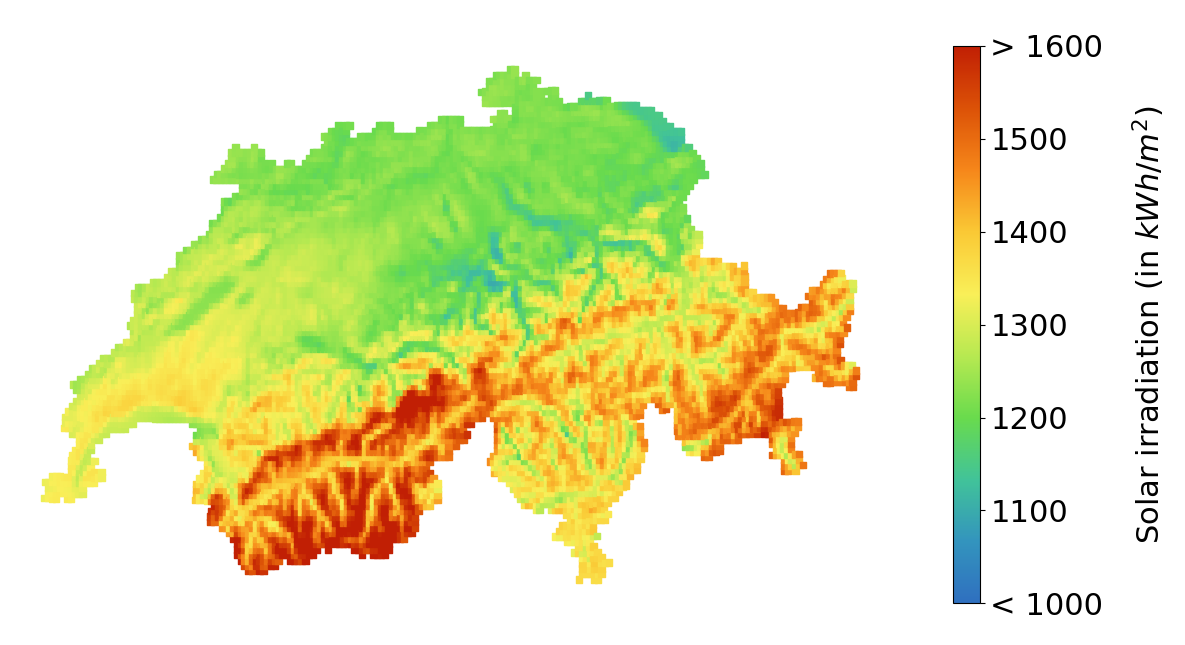
\includegraphics[width=\linewidth]{Figs/yr_raw.png}  
  \caption{}
  \label{figa:GHI_patterns}
\end{subfigure}
\begin{subfigure}{.49\textwidth}
  \centering
  % include first image
  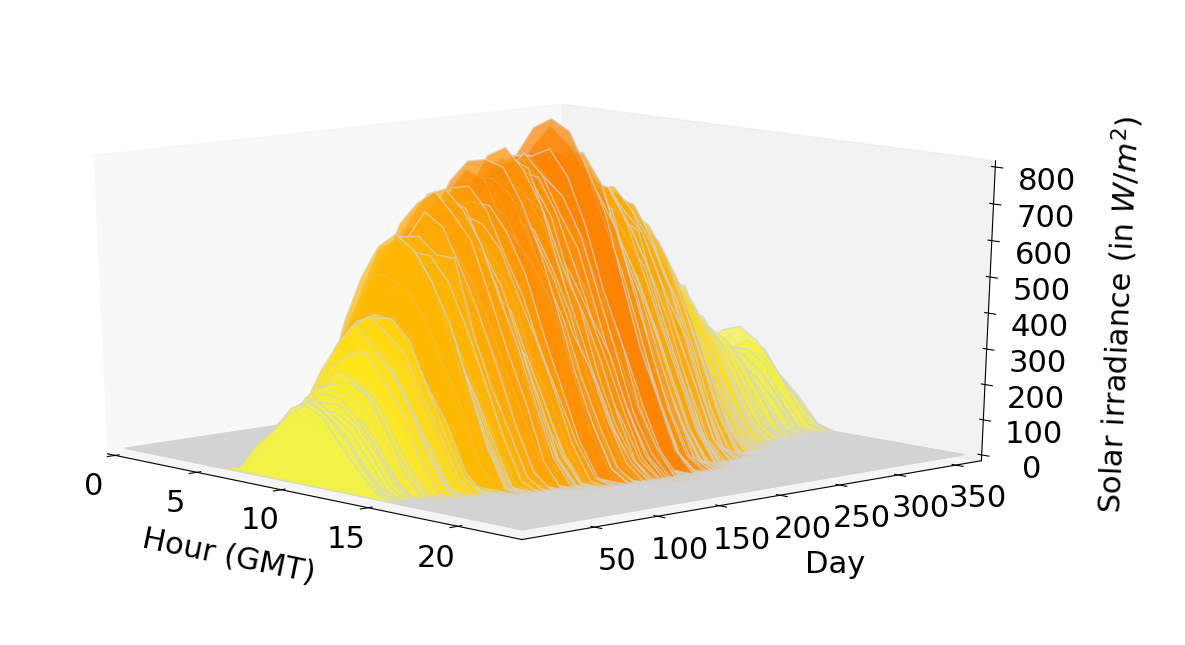
\includegraphics[width=\linewidth]{Figs/hours.png}  
  \caption{}
  \label{figb:GHI_patterns}
\end{subfigure}
\caption{(a) Yearly global solar irradiation from satellite data, (b) hourly distribution of global solar radiation at selected location, averaged for 2004-2015.}
\label{fig:GHI_patterns}
\end{figure}

% SOURCE: PV paper (original draft)
\textbf{Global and direct horizontal radiatio (GHI/DIR).} To estimate RPV potential for Switzerland, we use satellite data for global horizontal radiation (GHI), also known as surface incoming shortwave radiation, and direct beam radiation (DIR) provided by MeteoSwiss\cite{stockli_daily_2013}. The radiation describes the total solar power at the earth's surface, given in W/m$^2$. The solar energy is referred to as irradiation, given in Wh/m$^2$. The data are available as hourly values for the period from 2004-2015 on a longitude-latitude grid of 1.25 degree minutes, equivalent to approximately $1.6 \times 2.3$ km$^2$ (see Fig.~\ref{figa:GHI_patterns}).  
\nomenclature[A]{GHI}{Global horizontal radiation}
\nomenclature[A]{DIR}{Direct beam radiation}

We average the 12 years of satellite data in order to obtain an average year in hourly resolution, i.e. $12 \times 365$ time steps for 11,243 satellite pixels (see Fig.~\ref{figb:GHI_patterns}). This reduces the variability of the radiation data, and furthermore allows the estimation of long-term RPV potential without bias due to extreme meteorological events of a specific year. Furthermore, all hours with constantly zero GHI measurements are removed (i.e. night hours). The remaining 10-17 day hours result in $\sim~3-6$ million hourly values for GHI and DIR per month, depending on the month. 

\textbf{Surface albedo.} A dataset for surface reflectance, also referred to as surface albedo, is available at the same spatio-temporal resolution as the global and direct horizontal radiation. In particular in Switzerland, where a large part of the country is covered by mountains, the surface albedo plays an important role in the quantification of the reflected solar radiation component \cite{kahl_bright_2019}. As the surface albedo shows low variations throughout the day, the data is aggregated to daily values, before being averaged across the 12 years as described above. 

All solar radiation data has been derived by MeteoSwiss from Meteosat Second Generation (MSG) satellite observations using the Heliomont algorithm~\cite{stockli_heliomont_2017}. It was developed to improve the quality of the results, particularly in Switzerland's Alpine territories. 
\citet{ineichen_long_2014} performed a comprehensive validation of various satellite-based products against measurement data, and found a negligible bias of the hourly satellite data across 18 measurement stations. 
The standard deviation for hourly global and direct radiation is 19\% and 39\%, respectively.

\subsection{Temperature}

\textbf{Maximum daily air temperature.} Air temperature data, including the daily mean, maximum and minimum air temperature, is available from MeteoSwiss on a grid of $1 \times 1$ km$^2$ for Switzerland \cite{meteoswiss_daily_2017}. 
In contrast to the solar radiation, MeteoSwiss uses near-surface air temperature measurements from meteorological stations, which are interpolated in three dimensions, with further adjustments to account for temperatures in high mountain areas \cite{meteoswiss_daily_2017}.
For coherence with the solar radiation data described above, we collect daily air temperature data for the years of $2004-2015$. 
We use maximum air temperature in the estimation of RPV potential (Chapter~\ref{solar}) as the maximum solar yield occurs around midday when temperatures are near their daily maximum, resulting in a conservative estimate of the PV panel efficiency.

\textbf{Heating degree days (HDD).}
\label{app:HDD}
The HDD is defined in the norm SIA 2028 as the sum of the heating degrees for each month $m$, averaged across 20 years, such that \cite{sia_klimadaten_2010}: 

\begin{equation}
\label{eq:hdd}
    HDD = \frac{1}{20} \sum_{y=1}^{20} \sum_{d=1}^{d_m} (20 - T_{m}(d, m, y)) \quad \forall T_{m} (d, m, y) \leq 12 ^\circ C. 
\end{equation}

where $d_m$ is the number of days of each month and $T_{m}$ is the daily mean temperature on day $d$ in month $m$ of year $y$. 
We use gridded daily mean air temperature data for 20 years ($1991-2011$) \cite{meteoswiss_daily_2017} to compute the HDD for each of the $1 \times 1$  km$^2$ pixels of the temperature grid (see above). The time span of  $1991-2011$ is chosen such as to yield results that are comparable to the tabulated HDD in \cite{sia_klimadaten_2010}.
The HDD is then spatially interpolated to a resolution of $200 \times 200$ m$^2$ using a Random Forest algorithm (see Section \ref{RF}) with the pixel coordinates and the altitude (obtained from DTM) as features.

\textbf{Cooling degree days (CDD).} In contrast to the HDD, no Swiss norm exists for the computation of CDD. We hence obtain the CDD from \cite{christenson_climate_2006} using a reference temperature of $18 ^\circ C$:
\begin{equation}
\label{eq:cdd}
    CDD = \frac{1}{20} \sum_{y=1}^{20} \sum_{d=1}^{d_m} (T_{m}(d, m, y)-18) \quad \forall T_{m} (d, m, y) \geq 18 ^\circ C. 
\end{equation}
for the same timespan ($1991-2011$) and spatial resolution ($1 \times 1$ km$^2$) as the HDD, which is then interpolated to pixels of $200 \times 200$ m$^2$ as described above.

\section{Subsurface data [\textit{PRELIMINARY}]}
\label{data_geo}

The geothermal cadastres, provided by ASIT-VD \cite{asit_vd_cadastre_2019-1} and SITG \cite{sitg_cadastre_2019}, contain information on (i) restriction zones for geothermal installations within the case study area, (ii) thermal ground properties, and (iii) over 4,400 existing installations with $\sim 10,800$ BHEs.

\subsection{Geological characteristics}
\textbf{Geological Maps (GK500).}

\textbf{Depth of unconsolidated deposits.}

\subsection{Thermal ground properties}

\textbf{Thermal conductivity.}

\textbf{Thermal diffusivity.}
The ground data provided in the cadastres include the thermal conductivity ($\lambda$) and the heat capacity ($\rho C$, Geneva only), from which the diffusivity is obtained as $\alpha = \lambda / \rho C$ \cite{pahud_geothermal_2002}.
The $\lambda$ and $\rho C$ are computed as the average of the ground properties of each rock layer weighted by % weighted
its thickness, which is given by 3D models of the subsurface \cite{groupe_de_travail_pgg_evaluation_2011-1}.
The ground data exists for depths in the range of $50-300m$ as pixels of $50m$ spatial resolution in all 3 dimensions. 
Constrained by this spatial resolution and $H_{max}$, we obtain four scenarios for the borehole depth $H$ (see Table ~\ref{tab:data}).
To obtain $\lambda$ and $\rho C$ for all scenarios of $H$ in the entire study region, we compute any missing values as weighted averages using
tabulated data \cite{groupe_de_travail_pgg_evaluation_2011-1, sia_sondes_2010}. 
The resulting maps for $\lambda$ and $\alpha$ for a borehole depth of $H = 100m$ are shown in Fig. \ref{fig:lambda} and \ref{fig:alpha}.

\textbf{Ground temperature.}
The data for $T_0$ has been provided by \citet{assouline_machine_2019} for pixels of $200m$ resolution.
The data is estimated from ground measurements using Machine Learning \cite{assouline_machine_2019}.
To minimise the impact of the built environment on these measurements, we use the annual average ground temperature at a depth of $1m$.
Its interpolated values at the resolution of $\lambda$ and $\alpha$ is shown in Fig.~\ref{fig:T0}.
The temperature gradient in the Swiss plateau is approximately constant at $0.03K/m$ \cite{sia_sondes_2010}.

\subsection{Restrictions for geothermal installations}

The restriction zones are divided into three categories, shown in Fig.~\ref{fig:lims}, which indicate whether the installation of BHEs is permitted, limited, or prohibited.
Prohibited zones are excluded from the study. 
The permitted and limited zones are overlaid with information from existing installations to derive $H_{max}$, as no data on the allowed drilling depth is available.
Based on these considerations,
we choose $H_{max}$ as the $75^{th}$ percentile of the depth of the existing BHEs, yielding values of $200m$ and $150m$ for the "permitted" and "limited" zones, respectively. 

\cleardoublepage

\part{Spatio-temporal estimation of renewable energy potentials}
\label{potential}
\chapter{Solar energy potential}
\label{solar}

\vspace{-45pt} % one line spacing corresponds approx to 15 pts
\begin{tcolorbox}[enhanced,width=\textwidth,size=fbox,
        sharp corners,colframe=black!5!white,drop fuzzy shadow southeast,
        boxrule=3mm, parbox=false] % other options: fontupper=\large\bfseries
This chapter is based on the article \citep{walch_big_2020}:

\qquad \bibentry{walch_big_2020}

Several limitations and aspects of further work highlighted in \cite{walch_big_2020} are addressed based on the conference proceedings \cite{walch_critical_2019, walch_quantification_2021, castello_quantification_2021, walch_fast_2019}: 
% walch_spatio-temporal_2019,

% \quad \bibentry{walch_spatio-temporal_2019} - % \textit{Section~\ref{irrad}} 

\quad \bibentry{walch_critical_2019} - \textit{\textbf{Section~\ref{solar_comparison}}} 

\quad \bibentry{walch_quantification_2021} - \textit{\textbf{Section~\ref{scenario_EW}}} 

\quad \bibentry{castello_quantification_2021} - \textit{\textbf{Section~\ref{scenario_area}}} 

\quad \bibentry{walch_fast_2019} - \textit{\textbf{Section~\ref{solar_application}}} 
\end{tcolorbox}

% SOURCE: Introduction ICAE paper
\begin{comment}
We use an Extreme Learning Machine (ELM) ensemble algorithm that allows to predict solar irradiance at an hourly time granularity for a high spatial resolution ($250 \times 250$) m$^2$ grid over Switzerland and to estimate the uncertainty related to the model and the data. The main advantages of this algorithm are (i) its fast training time and (ii) its ability to learn and to model complex non-linear phenomena with the desired precision. Hence this algorithm is well suitable for the analysis and modelling of large datasets [6,9,10].
\end{comment}

As rooftop photovoltaic (RPV) electricity plays a key role in the decarbonisation of the Swiss energy sector (see Chapter \ref{intro_REN}), the development of a database of the RPV electricity generation potential at hourly temporal resolution for the Swiss building stock is one objective of this thesis.
This chapter presents a big data mining approach, shown in Figure \ref{fig:graphical_abstract_RPV}, to estimate these RPV potentials at the national scale for Switzerland. 
The presented work adapts state of the art methods for the assessment of RPV potential and quantifies and combines different sources of uncertainty, which are systematically propagated throughout the modelling process.
% The presented work adapts state of the art methods for the assessment of RPV potential and 
% further addresses the systematic propagation of uncertainties arising from the modelling process. 
%To this aim, we adapt state of the art methods for the assessment of RPV potential in order to quantify and combine different sources of uncertainty. 
We further use Machine Learning to incorporate data that is only partly available in Switzerland.

In the following, we review related literature on the large-scale estimation of RPV potential and its uncertainty (Section~\ref{solar_literature}), describe the big data mining methodology as proposed in \cite{walch_big_2020} (Section \ref{solar_method}) and present the results for Switzerland (Section \ref{solar_results}).
The method and results from Sections \ref{solar_method} and \ref{solar_results} are compared to those of five other studies of RPV potential for Switzerland (Section~\ref{solar_comparison}), and validated against real-world data in two case studies (Section \ref{solar_scenarios}). 
For the validation, we consider 
% Expanding on the method from Section \ref{solar_method}, we further  
% Addressing some of the limitations discussed in Chapter \ref{discussion_pv}, we 
two arrangements of PV panels on flat roofs, 
% which are validated against measurements, 
and propose an image-based approach to quantify the available area for PV panel installation. 
To motivate the application of the national-scale RPV potential dataset for studies in areas with similar geographic and meteorological conditions as Switzerland, we outline a Machine Learning approach to predict rooftop solar irradiation (Section \ref{solar_application}).
% An application of the national-scale RPV potential dataset for RPV studies in areas with similar geographic and meteorological conditions as Switzerland, based on a Machine Learning approach, is outlined in Section
% , and discuss the methodological and practical contributions and limitations of this study (Section \ref{discussion_pv}). 
% The resulting new scenarios for the RPV potential in Switzerland are compared and discussed in the context of the Swiss energy strategy. 
Finally, we discuss the methodological and practical contributions, limitations and applications of the work presented in this chapter (Section \ref{discussion_pv}) 
% outline a Machine Learning approach to use the data generated within this chapter for studies of RPV potential in areas with similar geographic and meteorological conditions (), 
and summarize the main findings (Section \ref{solar_conclusion}).
For reasons of coherence, some repetition with respect to  previous chapters is possible.

\begin{comment}
% SOURCE: PV Paper
The decarbonisation of the energy system plays an important role in fulfilling the ambitious emission targets set by the Paris Agreement \cite{peters_key_2017}. 
In this context, the large-scale deployment of rooftop-mounted photovoltaics (RPV) has attracted increasing attention in recent years \cite{jager-waldau_pv_2018}.
A quantitative assessment of the potential electricity generation from RPV is essential to formulate
%
effective incentive policies for their integration in the built environment. This requires accurate input data at a high spatial and temporal resolution in order to characterize regional differences and to assess the seasonal and intra-day variation of the generation \cite{bodis_high-resolution_2019}.
In addition, the analysis of RPV potential involves several uncertainties, which need to be quantified to facilitate interpretation of the results for policy making. 
 
Currently, there is no methodology that estimates the large-scale RPV potential at a high spatio-temporal resolution and also addresses the systematic propagation of uncertainties arising from the modelling process.
This paper contributes to fill this gap by adapting state of the art methods for the assessment of RPV potential in order to quantify and combine different sources of uncertainty. 
We further use Machine Learning to incorporate information that is only available in parts of the study region of Switzerland.

\end{comment}

\begin{figure}[tb]
\centering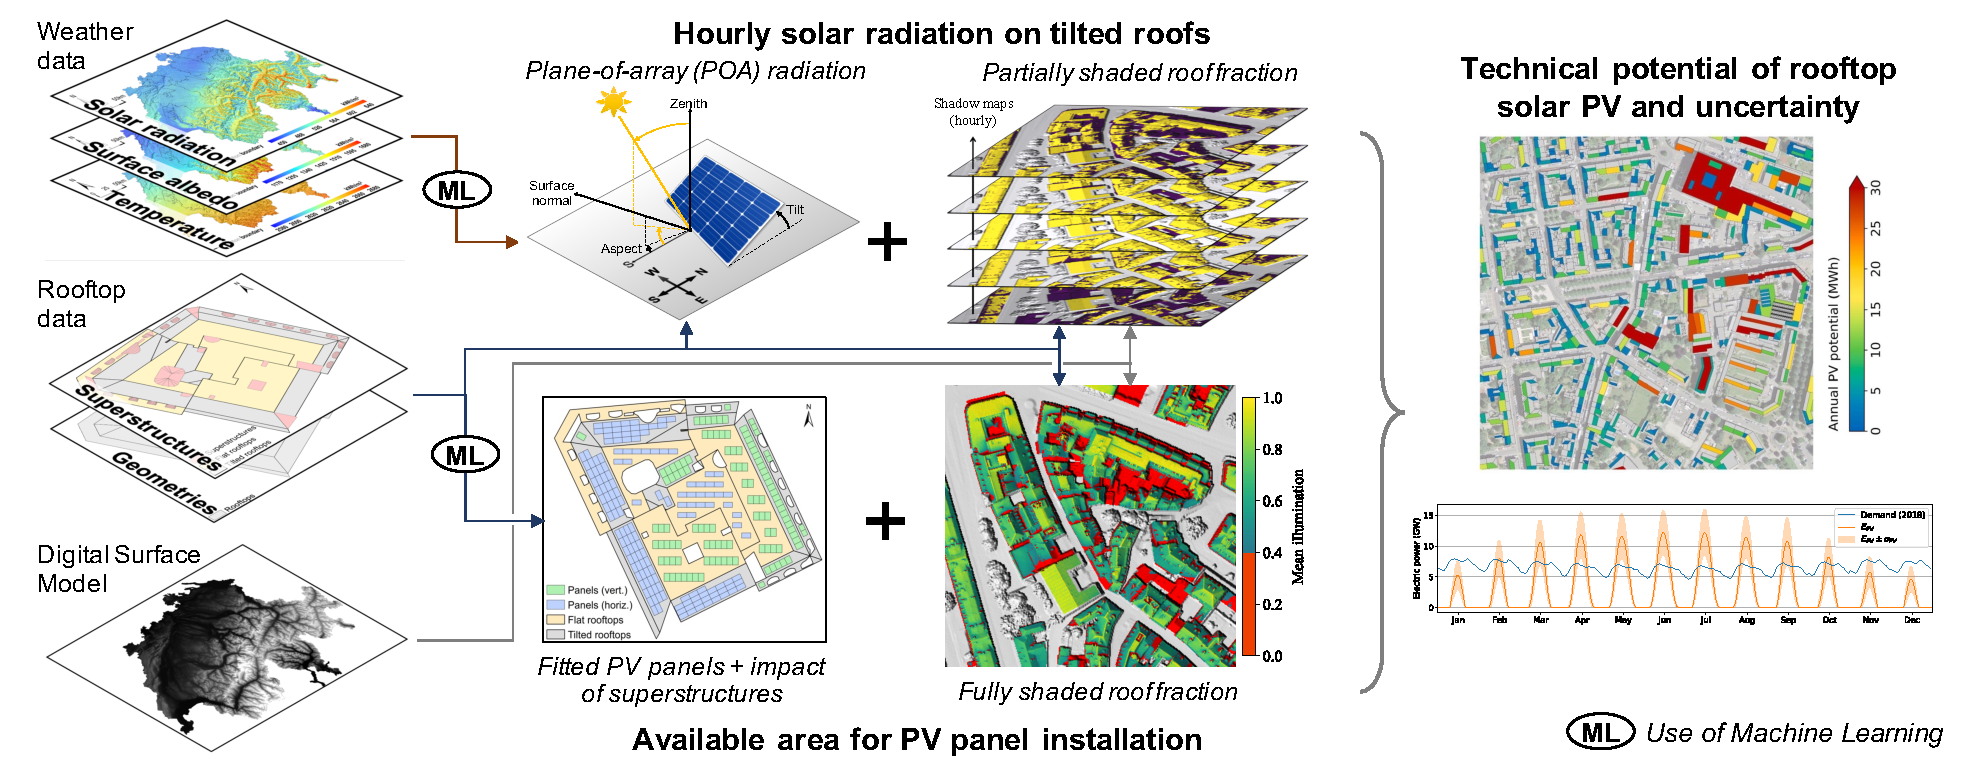
\includegraphics[width=1.0\linewidth]{Figs/graphical_abstract_RPV.pdf}
\caption{Graphical abstract for the large-scale estimation of hourly solar PV potential}
\label{fig:graphical_abstract_RPV}
\end{figure}

\section{Related literature}
\label{solar_literature}
% SOURCE: PV Paper
Constrained by the availability of building and environmental data at a high spatial resolution, most existing studies on RPV potential are carried out at district or city scale only, including case studies in the US \cite{levinson_solar_2009}, Canada \cite{nguyen_incorporating_2012}, Portugal~\cite{santos_applications_2014} or Germany \cite{strzalka_large_2012}. 
Few studies analyse an entire region or country, for example in the US \cite{phillips_data_2019, kodysh_methodology_2013}, Spain \cite{schallenberg-rodriguez_photovoltaic_2013}, or Saudia Arabia \cite{khan_rooftop_2017}. 
%
Many PV assessment studies use monthly or yearly solar radiation data in order to derive a large-scale PV potential \cite{ordonez_analysis_2010}. This data is used to quantify the available area to install PV \cite{mansouri_kouhestani_evaluating_2019} and to discuss the economic feasibility of PV scenarios \cite{romero_rodriguez_assessment_2017}.
While these granularities provide a relatively accurate estimation of the annual RPV potential, an hourly or higher temporal resolution is needed to assess the intra-day variation of the generation. Such temporal resolutions are used at the scale of cities or municipalities \cite{hong_development_2017, singh_estimation_2015} and serve to validate the estimations against measurements \cite{jakubiec_method_2013}, to compare PV technologies \cite{lukac_buildings_2014}, or to simulate energy systems with high shares of PV~\cite{wegertseder_combining_2016}. However, an hourly resolution is rarely used at regional or national scale, in which case the available area for PV is not addressed \cite{buffat_scalable_2018}.

Reasons for the lack of national-scale studies at an hourly temporal resolution are the computational challenges associated with the processing of the required input datasets as well as
the handling of missing data and data that is not available in the entire study region.
State of the art data processing techniques for estimating RPV potentials include physical models, geographic information systems (GIS), image processing and Machine Learning (ML). 
Physical models are used to compute the solar radiation on tilted surfaces, as well as the module and inverter efficiencies \cite{ramirez_camargo_spatio-temporal_2015}. 
GIS is applied to estimate shading effects and the sky view factor \cite{klauser_solarpotentialanalyse_2016, desthieux_solar_2018}.
The available area for installing PV is estimated in some studies using image recognition \cite{mainzer_assessment_2017, palmer_gis-based_2018}, while other methods use ML \cite{assouline_quantifying_2017, assouline_large-scale_2018}. 
These recent advances enable the integration of all mentioned aspects in high-resolution PV assessments at the national scale.
%
Missing data, in particular for predicting the available area for installing PV, is typically handled using constant coefficients and expert knowledge \cite{iea_potential_2002} or sampling techniques~\cite{wiginton_quantifying_2010}. Data with partial spatial coverage, i.e. information that is available only in parts of the study area, is successfully used in \cite{assouline_quantifying_2017, assouline_large-scale_2018} by applying ML. 
This method can be further improved by using different urban features and a larger training dataset.

To date, little research has quantified uncertainties for RPV potential assessments. Some studies address the uncertainties related to photovoltaic yield predictions for individual case studies \cite{thevenard_estimating_2013, gueymard_direct_2009}. In large-scale studies, confidence intervals are used in \cite{buffat_scalable_2018} to quantify the uncertainty related to the solar radiation, while they are used in \cite{assouline_large-scale_2018} to assess the available area for installing PV. 
The combination of different sources of uncertainty has been addressed through a scenario-based analysis for a local case study \cite{kreifels_uncertainty_2016} or by means of a sensitivity analysis \cite{martins_sensitivity_2016}. \citet{izquierdo_method_2008} provide a statistical propagation of uncertainty, which however focuses only on the available area for PV installation.
To the best of our knowledge, currently no methodology exists which quantifies and combines different sources of uncertainty related to the solar radiation and the available area that yields an uncertainty estimate on the technical RPV potential.

Our big data mining approach contributes to the existing literature by providing a methodology for a large-scale RPV potential and uncertainty estimation in hourly temporal resolution and a spatial resolution of individual roof surfaces. 
For this purpose, we combine state of the art physical models and GIS processing techniques with ML, 
which allows us to extract useful information from data that is only available in parts of the study area.
Our approach is used to quantify
(i) the spatio-temporal variation of the horizontal radiation, 
(ii) the effects of surrounding trees and buildings on roof shading and the sky view factor, 
(iii) the impact of roof geometry and roof superstructures, for example dormers and chimneys, on the available area for installing PV panels, 
and (iv) the temperature dependence of the PV module efficiency. 
We further present a systematic quantification of the uncertainties by treating each variable involved in the modelling process as a randomly distributed variable.
This allows to combine the uncertainties using their statistical distribution in order to obtain a total uncertainty on the technical potential estimate. 
The application of our method to 3.7 million buildings in Switzerland results in the first national-scale dataset of PV potential and uncertainty in hourly temporal resolution for individual rooftops. 

\begin{comment}
The paper is structured as follows. 
Section~\ref{data} introduces the datasets used in the study. 
Section~\ref{workflow_PV} describes the methodology for the computation of the RPV potential and the uncertainty propagation.
Section~\ref{solar_results} presents the results of the individual processing steps as well as the final technical RPV potential. A sensitivity analysis is performed to identify the most impactful steps of the estimation process.
Section~\ref{discussion_pv} discusses the methodological and practical contribution of the work and outlines its limitations and applications. 
Section~\ref{solar_conclusion} presents the conclusions and gives an outlook to future applications of the developed method.
\end{comment}

\begin{comment}
% SOURCE: Introduction ICAE paper
Current climate and environmental policies in Switzerland and worldwide aim at a strong reduction of CO$_{2}$ emissions in the next decades by transitioning from fossil fuels to renewable energy. Harvesting solar energy using photovoltaic (PV) and solar thermal technologies is one promising approach to achieve the ambitious emission targets. To determine the potential for large-scale deployment of solar technologies and to assess the requirements for a successful integration into the built environment, an accurate modelling of the spatial and temporal patterns of solar irradiance is essential. In this study, we present a methodology for modelling environmental variables at high spatial and temporal resolution by using large satellite datasets. We apply it to predict hourly global horizontal irradiance (GHI) on a ($250 \times 250$) m$^2$ grid, in order to be able to estimate PV potential at the neighborhood scale in Switzerland. 
Several data-driven methods exist to model solar irradiance. These include averaging the nearest neighbors [1], geostatistical methods such as kriging [2] as well as machine learning approaches such as Support Vector Machines [3], Random Forests [4] and neural networks [5,6]. As averaging tends to oversimplify the modelling, and kriging is computationally intensive and requires modelling of anisotropic spatial correlations and stationarity of the process, the data-driven machine learning algorithms have recently gained much attention due to their performance and speed [7]. Most studies however focus either on a high spatial or temporal resolution and frequently do not consider the uncertainty that is intrinsic to the modelling [8]. 

% SOURCE: Research plan
Several methods exist in the literature to map horizontal irradiance to obtain a physical solar energy potential. These include averaging the nearest neighbours [5], geostatistical methods such as kriging [18], [19] as well as machine learning approaches such as Support Vector Machines [3], Random Forests [20] and neural networks [21]–[23]. As averaging tends to oversimplify the modelling, and kriging is computationally intensive and requires modelling of anisotropic spatial correlations and stationarity of the process, the data-driven machine learning algorithms have recently gained much attention due to their performance and speed [24]. Most models do not estimate the uncertainty related to modelling horizontal irradiance, which is an important aspect if the results are processed further.
For an estimation of the geographic potential in urban environments, the most significant factors are shading effects and the determination of the area available for the installations [3]. Several methods exist to compute these in a detailed fashion, including image analysis and 3D modelling [25]. There are two main issues with computing urban factors for a large geographic area: 1) high-resolution datasets are typically not available everywhere, and 2) the computational time for exact methods is prohibitively high [7]. Different methods exist to approximate urban factors. These range from using standard tabulated factors based on expert opinions [26], statistical methods [7] and extrapolation techniques based on Machine Learning [3]. Assouline et al. [14] provide a detailed analysis of these methods. 
\end{comment}

\section{Methodology}
\label{solar_method}

\begin{figure}[tb]
\centering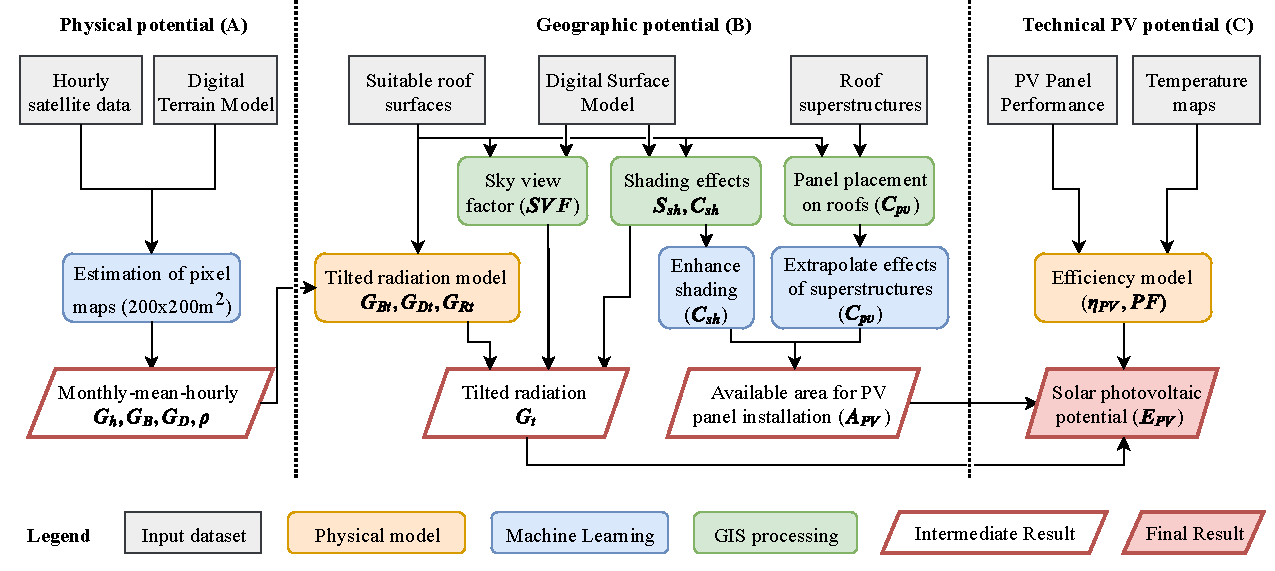
\includegraphics[width=1.0\linewidth]{Figs/solar_workflow.pdf}
\caption{Workflow for modelling of hourly solar PV potential. \textit{Input datasets }are described in Chapter~\ref{data}. \textit{Physical models} are provided in Chapter~\ref{phys_models}. \textit{Machine Learning} algorithms are summarised in Chapter~\ref{ML_supervised}. \textit{Geospatial (GIS) processing} methods are introduced in Chapter~\ref{GIS_methods}.}
\label{fig:workflow_PV}
\end{figure}

To estimate the RPV potential and its uncertainty, we propose a methodology that combines Machine Learning, GIS processing and physical models for the treatment of large spatio-temporal datasets, such as those presented in Chapter~\ref{data}.
Uncertainties are quantified from the statistical distribution of the variables involved in the potential estimation in the form of standard deviations.
They are assessed for various modelling steps and combined in order to obtain an uncertainty on the PV potential.

The method, illustrated in Fig. \ref{fig:workflow_PV}, is based entirely on open-source software and adopts the hierarchical approach summarized in Chapter~\ref{method_solar_hierarchy}. Its steps include 
(i) the \textit{physical potential}, driven by the horizontal solar radiation, 
(ii) the \textit{geographic potential}, accounting for the impact of the built environment, and
(iii) the \textit{technical potential}, defined as the potential electricity generation.
The variables involved in each stage of the model and their relationships are explained below. The following subsections will detail the methodological contributions for the individual processing steps and the proposed quantification of uncertainty.

The physical potential is defined as the horizontal solar radiation at the earth's surface ($G_h$) for each time step $t$. The $G_h$ is composed of a direct beam component ($G_B$) and a diffuse component ($G_D$) such that \cite{loutzenhiser_empirical_2007}:

\begin{equation}
\label{eq:Gh}
G_{h}(t) = G_{B}(t) + G_{D}(t)
\end{equation}

The horizontal radiation is computed at a monthly-mean hourly (MMH) temporal resolution and a spatial resolution of $200 \times 200$ m$^2$, 
which is chosen as a trade-off between topographic detail and computational complexity as suggested in \cite{izquierdo_method_2008, assouline_large-scale_2018}. 
Each MMH time step represents an average value at a given hour of each month, across all days of the month. This leads to 288 distinct time steps, i.e. 24 hours for each of the 12 months. 
Using MMH values instead of 8760 hourly time steps allows to reduce the computational cost by a factor of 30, while preserving the daily and seasonal patterns of the average PV potential.
Any deviation from the MMH values is however covered by their uncertainty.

The geographic potential accounts for the rooftop geometry, for superstructures, for shading effects and for the sky visibility. It is estimated for each roof surface considering the tilted radiation ($G_t$) and the available roof area for PV panel installation ($A_{PV}$)  \cite{assouline_large-scale_2018}, such that:

\begin{equation}
\label{eq:irrad}
% G_{t}(t) = (1-S_{sh}(t)) * R_{B}(t)  G_{B}(t) + SVF * R_D(t)  G_{D}(t) + R_R(t)  G_h(t)
G_{t}(t) = (1-S_{sh}(t)) * G_{Bt}(t) + \mathit{SVF} * G_{Dt}(t) + G_{Rt}(t)
\end{equation}
\begin{equation}
\label{eq:area}
A_{PV} = A_{t} * C_{\mathit{pv}} * (1 - C_{sh})
\end{equation}

where $G_{Bt}$, $G_{Dt}$ and $G_{Rt}$ are direct, diffuse and reflected tilted radiation components, $\mathit{SVF}$ is the sky view factor, $A_{t}$ is the tilted roof area, $C_{\mathit{pv}}$ referred to as the \textit{panelled area coefficient} and $C_{sh}$ and $S_{sh}$ are referred to as the \textit{shaded area coefficient} and the \textit{hourly shading fraction} of the unshaded area, respectively.
%
The $C_{sh}$ represents the fraction of roof surface that is unshaded in less than 40\% of the daylight hours and is hence unsuitable for PV installation (see Section~\ref{shade}). The $S_{sh}(t)$ denotes the portion of the remaining roof area ($1 - C_{sh}$) that is shaded at each time step $t$. 
We treat $C_{sh}$ and $C_{\mathit{pv}}$, the proportion of roof area available to install PV panels, as independent factors. They are separately computed and it is assumed that no relevant overlap exists between the two factors. 
%
State of the art hourly physical models, described in Chapter~\ref{app:efficiency} (orange boxes in Fig.~\ref{fig:workflow_PV}), are used to obtain the tilted radiation components ($G_{Bt}, G_{Dt}, G_{Rt}$) 
We use the anisotropic Perez model \cite{perez_modeling_1990} to estimate $G_{Dt}$ , which is the overall most accurate diffuse radiation model \cite{noorian_evaluation_2008, loutzenhiser_empirical_2007}. 
The $G_{Rt}$ is computed using monthly mean albedo data (see Section~\ref{irrad}). This allows to account for snow cover in high-altitude locations, where a large albedo increases the PV production on steep roofs~\cite{kahl_bright_2019}.

The technical potential ($E_{PV}$) is the electricity output of each roof surface. It is obtained from the geographic potential, the panel efficiency ($\eta_{PV}$) and the performance factor ($\mathit{PF}$), which accounts for inverter efficiency and other losses such as soiling or degradation, such that \cite{assouline_large-scale_2018}:

\begin{equation}
\label{eq:pv}
E_{PV} = G_t(t) * A_{PV} * \eta_{PV}(t) * \mathit{PF}(t)
\end{equation}
The module efficiency and performance factor are calculated for each time step $t$ from the tilted radiation and the ambient temperature using the \textit{PVWatts} model~\cite{dobos_pvwatts_2014} detailed in Chapter \ref{app:efficiency}. We use daily maximum temperature (see Table~\ref{tab:meteo}) to obtain a conservative estimate of the panel efficiency. 

Table \ref{tab:vars} summarizes the variables used above and the method applied to model each of them. 

\begin{table}[tb]
\centering
\footnotesize
\caption{Summary of the parameters used in the estimation of technical RPV potential. The dimension refers to $P$ for pixels of $200 \times 200$ m$^2$, $R$ for roof surfaces and $t$ for time steps. PM denotes the use of physical models.}
\label{tab:vars}
\begin{tabular} {lccccccc} % X[-1,c] X[-1,c] X[-1,c]
\hline 
  & $G_{h,B,D}$ & $G_{Bt,Dt,Rt}$ & $S_{sh}$   & $\mathit{SVF}$  & $C_{sh}$  & $C_{\mathit{pv}}$ & $\eta_{PV}, \mathit{PF}$     
  \\
\hline 
Dimension & $P \times t$ & $R \times t$ & $R \times t$ & $R$   & $R$     & $R$      & $R \times t$  
\\
Unit     & W/m$^2$    & W/m$^2$  & -                          & -                  & -                    & -                     & -                             
\\
Method      & ML & PM & GIS & GIS & GIS+ML & GIS+ML & PM \\
Thesis section      & \ref{irrad}  & \ref{app:irrad}     & \ref{shade}       & \ref{svf} & \ref{shade} & \ref{panels} & \ref{app:efficiency} 
\\  
\hline 
\end{tabular}
\end{table}

\begin{comment}
\subsection{Physical models}
\label{phys_models}

State of the art hourly physical models are used to (i) obtain the tilted radiation components ($G_{Bt}, G_{Dt}, G_{Rt}$) and (ii) to quantify the module and inverter efficiency. Both models, shown as orange boxes in Fig.~\ref{fig:workflow_PV}, are summarized in \ref{app:irrad}.
We use the anisotropic Perez model \cite{perez_modeling_1990} to estimate $G_{Dt}$ , which is the overall most accurate diffuse radiation model \cite{noorian_evaluation_2008, loutzenhiser_empirical_2007}. 
The $G_{Rt}$ is computed using monthly mean albedo data (see Section~\ref{irrad}). This allows to account for snow cover in high-altitude locations, where a large albedo significantly increases the PV production on steep roofs~\cite{kahl_bright_2019}.
The efficiencies are calculated for each time step $t$ from the tilted radiation and the ambient temperature using the \textit{PVWatts} model~\cite{dobos_pvwatts_2014}. We use daily maximum temperature (see Table~\ref{tab:meteo}) to obtain a conservative estimate of the panel efficiency. 


%%%%%%%%%%%%%%%%%%%%%%%%%%%%%%%%%%%%%%%%%%%%%%%%%%%%%%%

\subsection{Machine Learning}
\label{ML}

Machine Learning is used here  
(i) to obtain the horizontal radiation and the albedo at the $200 \times 200$ m$^2$ output grid from lower-resolution satellite data, 
(ii) to estimate the $C_{sh}$ and 
(iii) to account for the roof area covered by superstructures in the estimation of $C_{\mathit{pv}}$. 
We use supervised regression algorithms, which learn from a training set that contains pairs of inputs (features) and their known output values (targets). 
The models are then applied to predict unknown outputs for a new set of features.

We consider two ML algorithms, namely Random Forests (RF) \cite{breiman_random_2001} and Extreme Learning Machine Ensembles (ELM-E) \cite{huang_extreme_2006, wang_extreme_2015}. 
Both are ensemble algorithms which predict a target variable by averaging the results of multiple estimators (decision trees/ELMs) that have been trained on random re-samples of the training data \cite{breiman_bagging_1996}. 
Ensembles are well-suited for the estimaiton of uncertainties, which give a useful indication of the model's accuracy \cite{heskes_practical_1997}. 
%
The ELM-E is very efficient at modelling large datasets~\cite{de_freitas_viscondi_systematic_2019}, so we use this algorithm to estimate the hourly solar radiation and the monthly albedo. Preliminary work has shown that the RF outperforms the ELM-E for higher-dimensional datasets with less training data. The RF is hence used to estimate $C_{sh}$ and $C_{\mathit{pv}}$.

To optimize the performance of each ML model, it is necessary to firstly select its features, and secondly to choose the parameters defining the structure of each model through hyper-parameter tuning. 
In the following sections, we will focus on the feature selection and the performance of the optimized ML models. Information regarding the tuning of the algorithms is provided in \ref{app:tuning}.

%%%%%%%%%%%%%%%%%%%%%%%%%%%%%%%%%%%%%%%%%%%%%%%%%%%%%%%
\end{comment}

\subsection{Horizontal solar radiation and albedo}
\label{irrad}

We propose an ML-based approach to estimate the horizontal radiation and the surface albedo for pixel maps of $200 \times 200$ m$^2$ resolution, as presented in the blue box in Fig.~\ref{fig:workflow_PV}-A.
The ML models yield the global ($G_h$) and direct ($G_B$) horizontal radiation for each MMH time step $t$ and the albedo ($\rho$) as monthly mean values. 
The diffuse radiation ($G_D$) is obtained from the estimated $G_h$ and $G_B$ by applying Eq.~(\ref{eq:Gh}). 
Using ML, we can model complex spatial patterns while being more efficient than other spatial interpolation methods such as kriging~\cite{rehman_spatial_2000}. 

The targets for the ML models of $G_h$ and $G_B$ are the satellite-derived global and direct radiation, which are split into 12 monthly subsets (see Chapter~\ref{data_solarRad}).
The initially considered set of features are the mean hour of each month, the geographic coordinates (x, y) as well as several terrain features including altitude (z), terrain slope and curvature \cite{robert_spatial_2012} (see Table~\ref{tab:DTM_ftrs}). 
A DTM (Chapter \ref{data_DEM}) is used to derive these terrain features for the satellite data and for the $200 \times 200$ m$^2$ output grid. 
To better model the spatio-temporal patterns of $G_h$ and $G_B$, we analyze the spatial features for each time step using the RF feature importance score~\cite{pedregosa_scikit-learn:_2011}.
Figure \ref{fig:ftrs_phys} shows their pattern for the months of June and December.
The feature importance exhibits a strong intra-day variation for x, y and z, which may be explained by the impact of the Swiss alpine terrain. All other features have a low importance throughout the day, and including these in the model does not improve its performance further.
Four features are hence selected for the final model: hour, x, y, z.
Figure \ref{fig:ftrs_phys} refers to $G_h$, but $G_B$ shows a similar trend.

Separate ELM-E are trained for each month for $G_h$ and $G_B$. % For model training, the $G_h$ and $G_B$ for 80\% of the 11,243 satellite pixels ($\approx 9,000$) are used for training, while the rest are kept for the test set. 
Their tuning procedure and the resulting hyper-parameter values of the models are provided in Appendix \ref{app:tune_ELM}. 
Table \ref{tab:G_train} shows the MSE between the targets and predictions for a random 20\% of the satellite coordinates (test set), which are excluded from training.
% , while Fig.~ \ref{figc:ELM_training} shows the fit of the predictions and the targets ($G_h$ only). 
Each entry represents one trained monthly ELM-E.
The model performance is overall better for $G_h$ than for $G_B$, as it is harder to model $G_B$ from the given set of features.
% 
To estimate $\rho$ from the satellite-derived daily albedo measurements, we train one ELM-E with similar features as described above, namely x, y, z and month. The model is tuned in a similar fashion as that of $G_h$ and $G_B$ and yields a test MSE of 0.10, which lies in the range of the values obtained for $G_h$.

\begin{figure}[tb]
\centering
\begin{subfigure}{.4\textwidth}
  \centering
  % include second image
  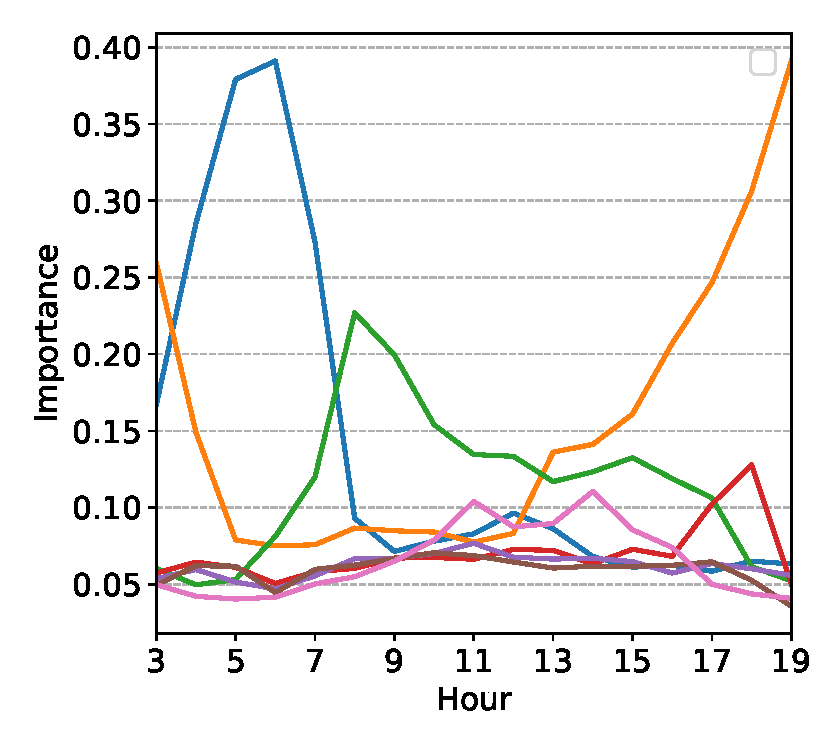
\includegraphics[width=\linewidth]{Figs/importance_July.pdf}  
\end{subfigure}
\begin{subfigure}{.4\textwidth}
  \centering
  % include first image
  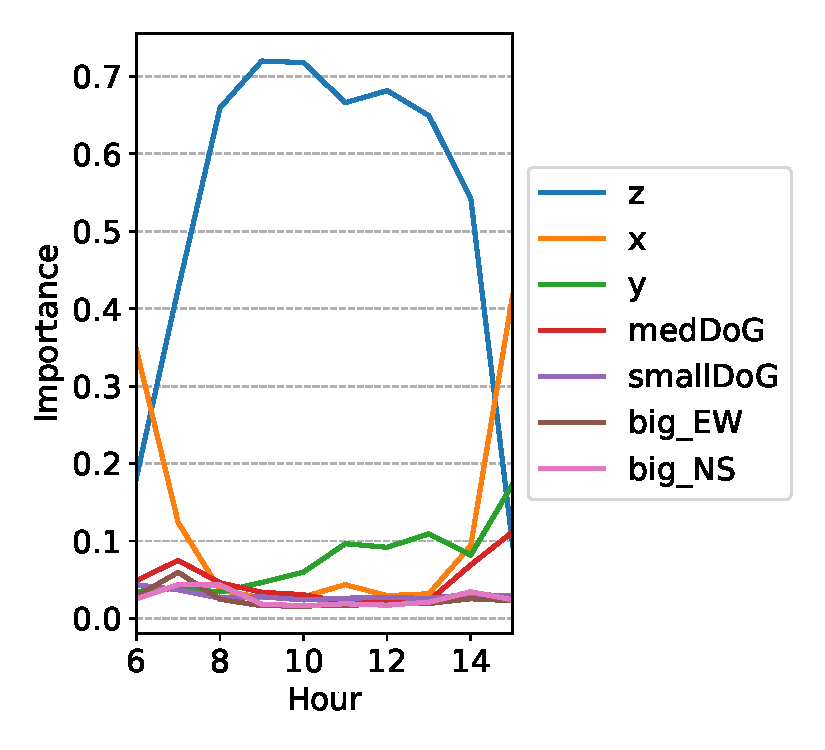
\includegraphics[width=\linewidth]{Figs/importance_December.pdf}  
\end{subfigure}
\caption{Feature importance per hour for $G_h$ for June (a) and December (b) for six terrain features, namely altitude (z), longitude (x), latitude (y), medium-scale curvature (medDoG), small-scale curvature (smallDoG), terrain slope in east-west (big\_EW) and north-south (big\_NS) direction.} %(c) Fit of predictions and targets for $G_h$ per month (test set) and the linear regression curve (black line) fitted on targets and predicted values.}
\label{fig:ftrs_phys}
\end{figure}

\begin{comment}
\begin{subfigure}{.32\textwidth}
  \centering
  % include second image
  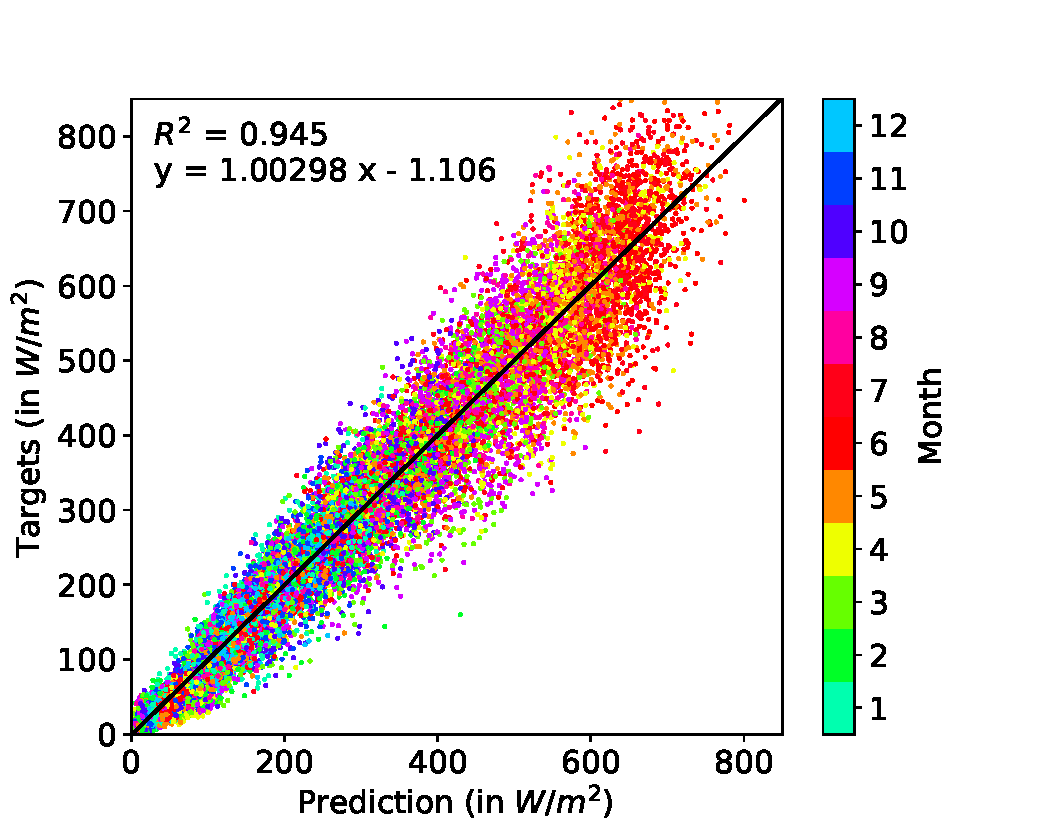
\includegraphics[width=\linewidth]{Figs/corr_test_data.pdf}  
  \caption{}
  \label{figc:ELM_training}
\end{subfigure}
\end{comment}

\begin{table}[tb]
\centering
\footnotesize
\caption{Test mean-squared error (MSE) for the estimation of $G_h$ and $G_B$.}
\label{tab:G_train}
\begin{tabular}{lcccccccccccc}
\hline 
 \textbf{MSE}   & Jan  & Feb  & Mar   & Apr   & May   & Jun   & Jul   & Aug   & Sep   & Oct  & Nov  & Dec  \\
\hline 
$G_h$  & 0.10 & 0.07 & 0.07  & 0.06  & 0.06  & 0.04  & 0.06  & 0.05  & 0.12  & 0.10 & 0.10 & 0.06 \\
$G_B$  & 0.17 & 0.12 & 0.18 & 0.17 & 0.21 & 0.14  & 0.18  & 0.12 & 0.26 & 0.16 & 0.21 & 0.11 \\
\hline 
\end{tabular}
\end{table}

%%%%%%%%%%%%%%%%%%%%%%%%%%%%%%%%%%%%%%%%%%%%%%%%%%%%%%%%%%%%%%%%%

\subsection{Available area for PV panel installation}
\label{panels}

The \textit{panelled area coefficient} $C_{\mathit{pv}}$ describes the available roof area for PV installation considering the roof geometry and superstructures. To compute $C_{\mathit{pv}}$, we use a geospatial algorithm in combination with ML, as represented by the green and blue box yielding $C_{\mathit{pv}}$ in Fig.~\ref{fig:workflow_PV}-B.
%
The geospatial algorithm, detailed in \ref{app:virtualPV}, virtually installs PV panels by projecting rectangular polygons onto the tilted roofs as shown in Fig.~\ref{fig:panels}. The $C_{\mathit{pv}}$ is then obtained from the number of installed panels.
The panels are installed in both horizontal and vertical alignments, as no alignment has technical advantages over the other and both are widespread. The configuration with a higher number of panels is selected for each roof.

\begin{figure}[tb]
\centering
\begin{subfigure}{.5\textwidth}
  \centering
  % include first image
  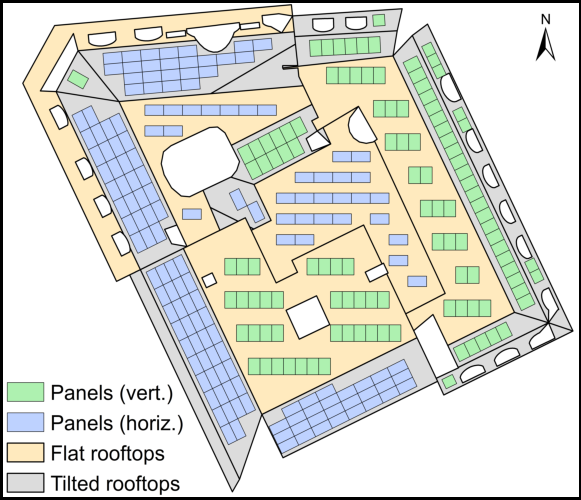
\includegraphics[width=.8\linewidth]{Figs/panels3.pdf}  
\end{subfigure}
\caption{Output of the virtual installation of PV panels after removing roof superstructures. The best configuration of vertically and horizontally oriented panels is selected. Panels on flat roofs are placed in south-facing rows and tilted at an optimal angle of 30$^\circ$.}
\label{fig:panels}
\end{figure}

The data on roof superstructures is however only available in one of Switzerland's 26 cantons (Geneva). We hence train an ML model to estimate the change in $C_{\mathit{pv}}$ due to the area covered by superstructures, which is applied to the rooftops of the remaining 25 cantons.
%
In our case, the training of the ML model is performed using the rooftop dataset with superstructure information in the Canton of Geneva (see Chapter~\ref{data_geometry}).
The fraction of their area on which virtual panels are installed provides the target for the ML algorithm ($C_{\mathit{pv}}^T$).
In addition, we define $C_{\mathit{pv}}^F$ as the fraction of the area on which virtual panels can be installed if no superstructures are removed from the roof polygons. This $C_{\mathit{pv}}^F$ is one feature of the ML model. %
The full set of the considered features is listed in Table \ref{tab:features}. 
Figure~\ref{fig:RF_Cpv} shows the feature importance for all inputs. 
While the top six features have the highest importance, 
the complete set of features is used for modelling $C_{\mathit{pv}}$ as this has been found to improve the estimation precision.

\begin{table}[b]
\centering
\footnotesize
\caption{Features considered in the ML models to estimate $C_{\mathit{pv}}$ and $C_{sh}$. $^1$The building density is computed as the number of building coordinates within a 100 m radius of each roof. $^2$The roof perimeter, shape index (perimeter per area) and vertex count are derived from the polygon data.}
\label{tab:features}
\begin{tabular}{lll}
\hline
\textbf{Computed features}               & \textbf{Roof features} & \textbf{Building features} \\
\hline
$C_{\mathit{pv}}^F$ / $C_{sh}^F$ & Tilted area                          & Footprint area                              \\
Panel tilt   & Tilt angle                          & Building type                              \\
(not used for $C_{sh}$)      & Aspect angle                        & Construction period          \\
Build. density$^1$                    & Perimeter$^2$                       & Number of floors                             \\
                                 & Shape index$^2$                       &   \\
 & Vertex count$^2$ & \\ 
\hline                                
\end{tabular}
\end{table}

Table~\ref{tab:errors_Cpv} reports the residuals between $C_{\mathit{pv}}^F$ and $C_{\mathit{pv}}^T$ (baseline), as well as the cross-validation error between the estimated $C_{\mathit{pv}}$ and the target $C_{\mathit{pv}}^T$ in the case of additive bias correction (MBE+) and for using the tuned RF model (see \ref{app:tune_RF} for details).
The bias correction is performed by adding the mean bias error (MBE) between $C_{\mathit{pv}}^F$ and $C_{\mathit{pv}}^T$  to all samples. 
We compare the root mean squared error (RMSE), mean absolute error (MAE), MBE and the R$^2$ coefficient of determination. All methods remove the negative baseline bias of 17\%. The RF outperforms the bias correction, as it achieves lower errors and a higher R$^2$. It is hence used to estimate the $C_{\mathit{pv}}$ used in Eq.~(\ref{eq:area}).

\begin{figure}[tb]
\centering
  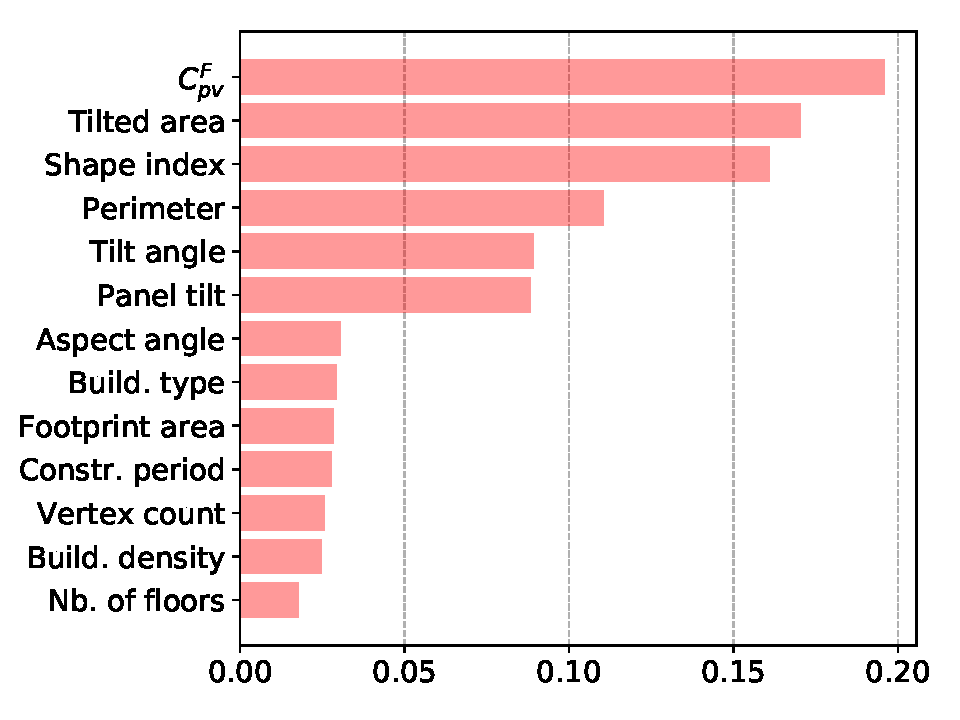
\includegraphics[width=.5\linewidth]{Figs/Feature_importance_panels.pdf}
\caption{Feature importance of all features considered for the estimation of $C_{\mathit{pv}}$.
}
\label{fig:RF_Cpv}
\end{figure}

\begin{table}[tb]
\centering
\footnotesize
\caption{Errors for estimating $C_{\mathit{pv}}$. We compare the residuals between $C_{\mathit{pv}}^F$ and $C_{\mathit{pv}}^T$ (baseline) with the cross-validation error between the estimated $C_{\mathit{pv}}$ and the target $C_{\mathit{pv}}^T$ in the case of bias correction (MBE+) and for using the Random Forest model (RF).}
\label{tab:errors_Cpv}
\begin{tabular}{lcccc}
\hline
      & \textbf{Baseline} & \textbf{MBE+}  & \textbf{RF}   \\ \hline
RMSE  & 0.23     & 0.15  & 0.12 \\
MAE   & 0.17     & 0.12  & 0.09 \\
MBE   & -0.17    & 0.00  & 0.00 \\
R$^2$ & -0.10    & 0.52  & 0.69 \\ \hline
\end{tabular}
\end{table}

%%%%%%%%%%%%%%%%%%%%%%%%%%%%%%%%%%%%%%%%%%%%%%%%%%%%%%%%%%%%%%%%%%%%%%%%%

\subsection{Shading effects and sky view factor}
\label{shade}
\label{svf}

To quantify shading effects from surrounding buildings and trees, we use a shadow casting approach \cite{buffat_scalable_2018, desthieux_solar_2018, klauser_solarpotentialanalyse_2016, ramirez_camargo_spatio-temporal_2015}. 
In contrast to the existing studies, we account for the shading effects in two ways:
First, strong shading effects may render parts of a roof unsuitable for installing PV. 
Second, some of the suitable area may be shaded at particular hours and reduce the PV potential for these hours. We hence distinguish between the \textit{shaded area coefficient} ($C_{sh}$), the fraction of roof area which is unsuitable due to shading, and the \textit{hourly shading fraction} ($S_{sh}(t)$), which is computed for each hour as the shaded portion of the remaining roof. 

The shadow casting approach (green box in Fig.~\ref{fig:workflow_PV}-B) models shadows on building roofs for each pixel of a DSM at a given sun position. It is used to produce hourly shadow maps for the representative day of each month (close to day 15~\cite{desthieux_solar_2018}) and hence yields results at the same temporal resolution as the solar radiation.
Figure~\ref{fig:horizons}a shows an example of these maps. They are binary maps, with a 0 (dark areas) representing a cast shadow and a 1 (yellow areas) indicating direct sun exposure. The shadow maps are averaged for all daylight hours, resulting in the mean illumination map shown in Fig.~\ref{fig:horizons}b. Its values represent the percentage of time steps for which each pixel is unshaded.

All areas with a mean illumination lower than the average value across all roofs (red areas) are considered unsuitable. 
We compute this average value as 42.7\% and hence use a rounded threshold of 40\% mean illumination to exclude unsuitable areas.
Dividing the red areas in Fig.~\ref{fig:horizons}b by the total roof area yields $C_{sh}$, while $S_{sh}$ is the fraction of zeros in Fig.~\ref{fig:horizons}a on the suitable (non-red) surfaces at time $t$. The GIS algorithm for shading effects is given in \ref{app:shade}. 

\begin{figure}[tb]
	\centering
	\begin{subfigure}{.52\textwidth}
		\centering
		% include first image
		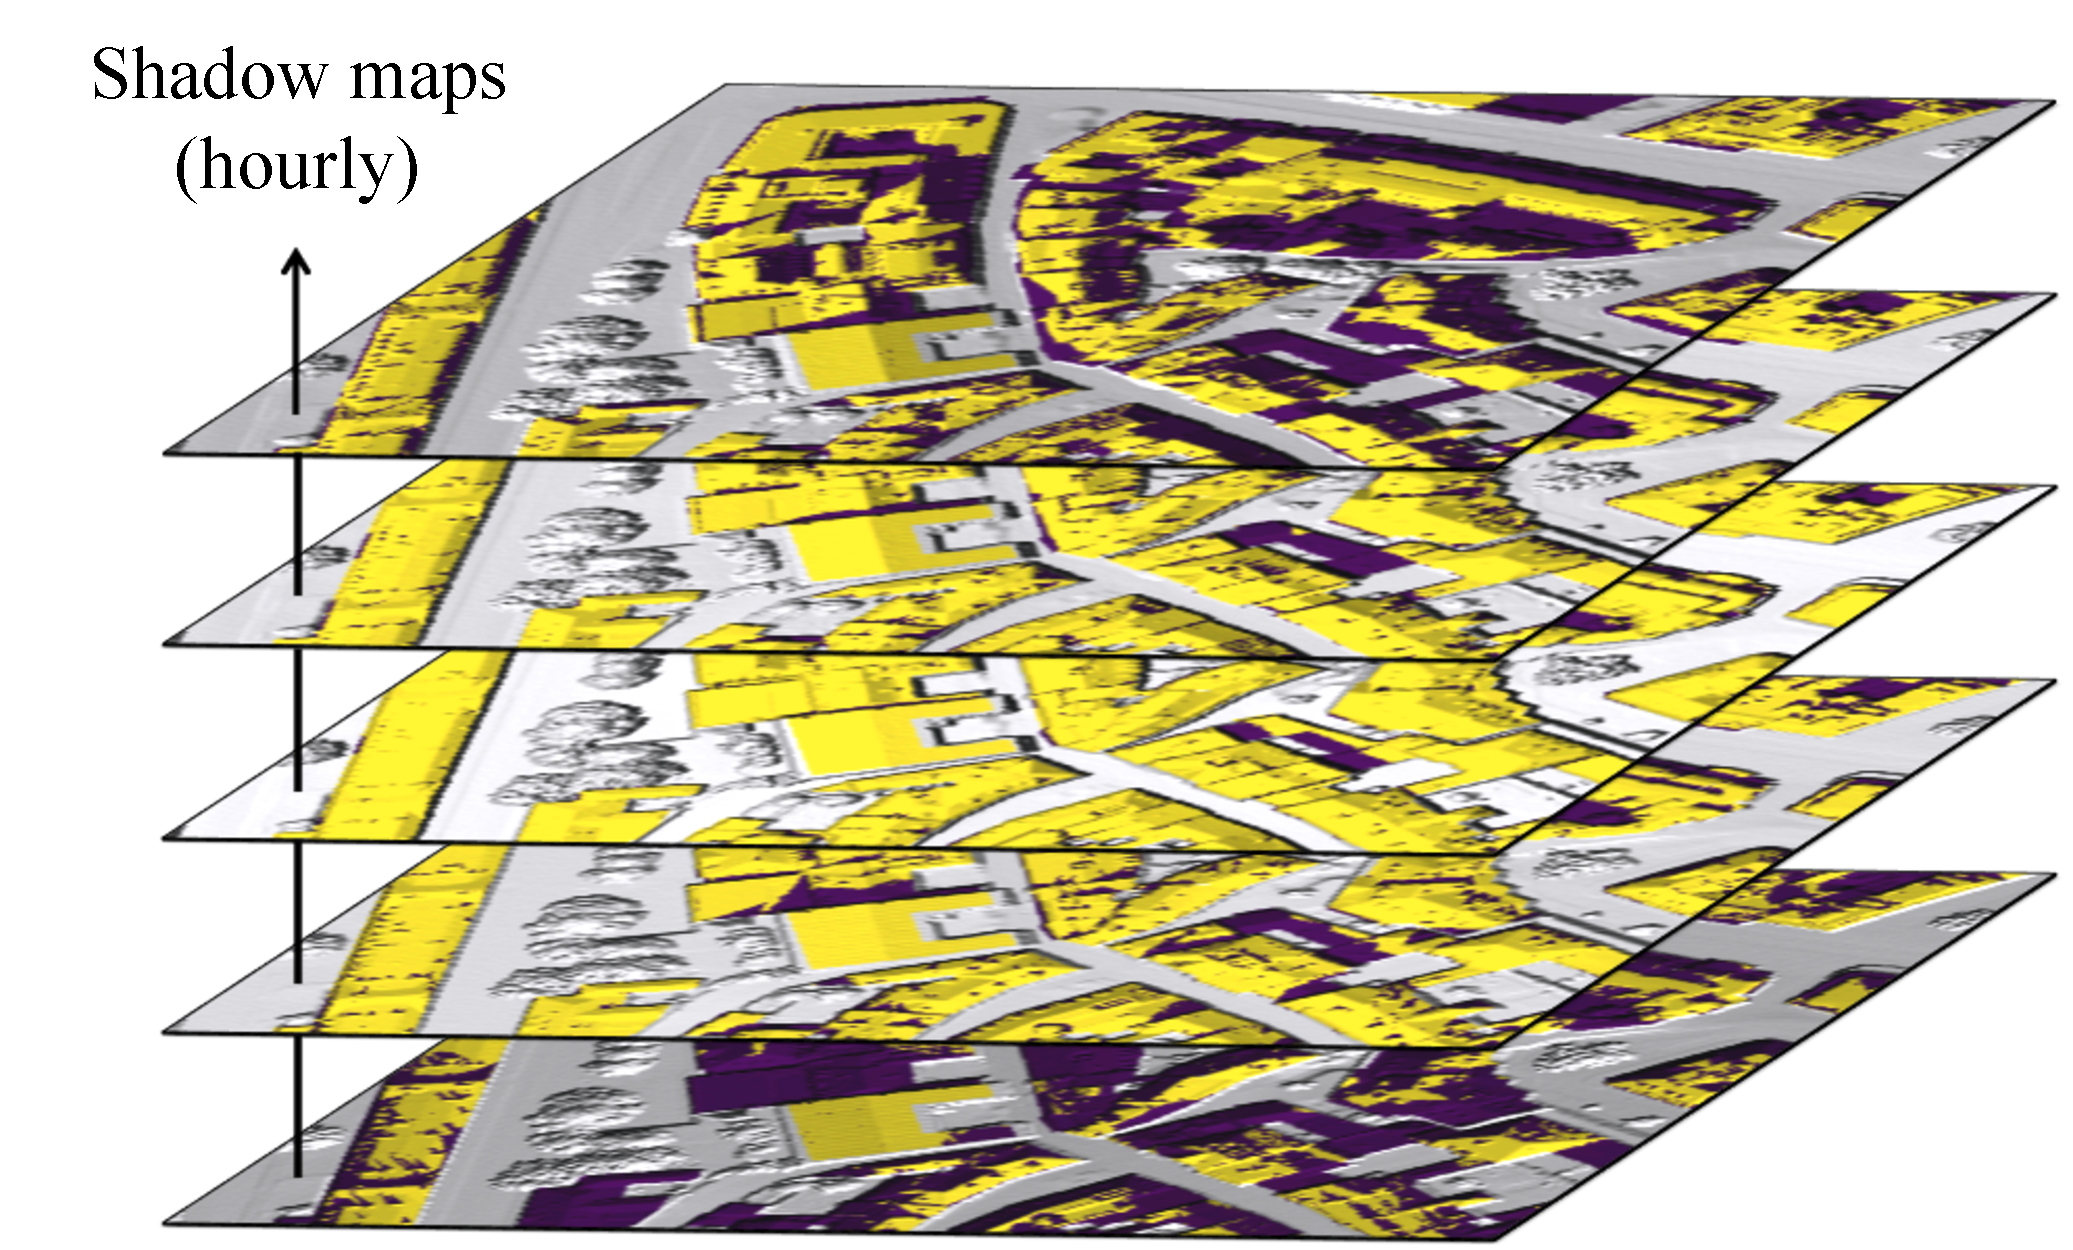
\includegraphics[trim=25 0 10 0, clip, width=.8\linewidth]{Figs/3d_shade.pdf} 
		\subcaption{}
	\end{subfigure}
	\begin{subfigure}{.44\textwidth}
		\centering
		% include first image
		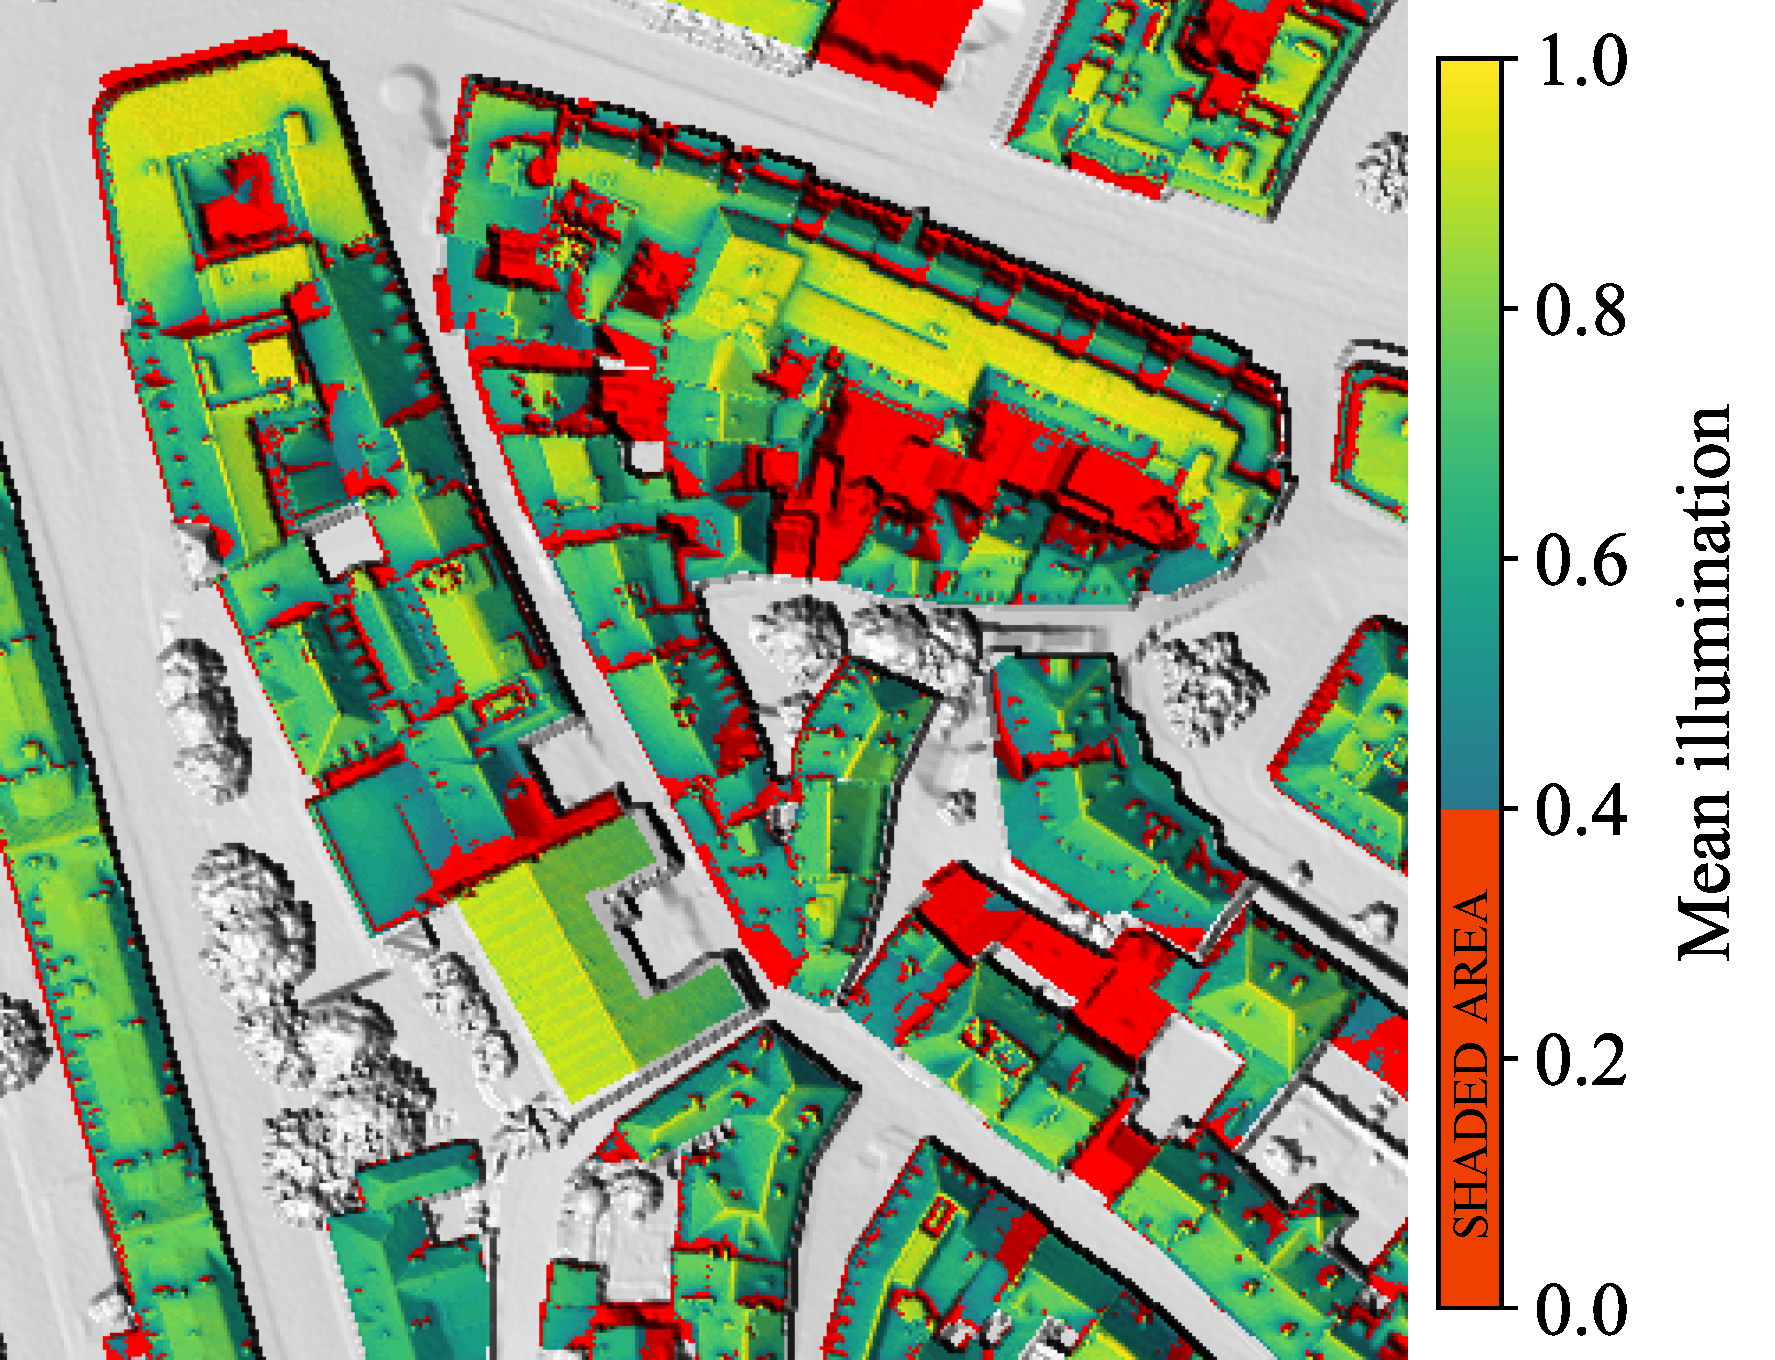
\includegraphics[width=.8\linewidth]{Figs/shade_mean.pdf}  
		\subcaption{}
	\end{subfigure}
	\caption{a) binary shadow maps used to derive $S_{sh}$, for 5 example time steps (0: cast shadow, 1: sun exposure). b) mean illumination map used to compute $C_{sh}$ (red areas).}
	\label{fig:horizons}
\end{figure}

Two datasets are available to compute $C_{sh}$ and $S_{sh}$: the national DSM$_{2\text{m}}$ and the DSM$_{50\text{cm}}$ for the canton of Geneva (see Table~\ref{tab:bld_landscape}). Our method aims at enhancing the national-scale $C_{sh}$ and $S_{sh}$ from the DSM$_{2\text{m}}$ based on knowledge extracted from the DSM$_{50\text{cm}}$, which is more recent and detailed. For this task, we denote the values extracted from the DSM$_{2\text{m}}$ as $C_{sh}^F$, $S_{sh}^F$ (features) and those obtained from the DSM$_{50\text{cm}}$ as $C_{sh}^T$, $S_{sh}^T$ (targets).
%
Their comparison yields an MBE of 2.7\% between $S_{sh}^F$ and $S_{sh}^T$ and of 8.9\% between $C_{sh}^F$ and $C_{sh}^T$. As the MBE for $S_{sh}$ is small compared to the order of magnitude of other uncertainties, we use an additive bias correction (MBE+) to correct $S_{sh}^F$ at the national scale, applied separately for each time step. 

The $C_{sh}$ shows a larger bias, so $C_{sh}^F$ systematically underestimates the shaded area coefficient. This leads to an overestimation of available area. 
As a mean bias correction (MBE+) increases the MAE (see Table~\ref{tab:errors_Csh}), we apply an ML model (RF) to estimate $C_{sh}$, illustrated by the blue box yielding $C_{sh}$ in Fig.~\ref{fig:workflow_PV}-B. 
The features that are used to estimate  $C_{sh}$ are listed in Table~\ref{tab:features}.
Figure~\ref{fig:RF_Csh} shows the feature importance for $C_{sh}$. Interestingly, the building type has a high importance. This may be due to the different objects that cause shading on buildings. 

The errors for estimating $C_{sh}$ are shown in Table~\ref{tab:errors_Csh}. While the improvement of the MAE when using ML is relatively small, we do observe a large improvement in the R$^2$ coefficient.
Unpredictable factors, such as discrepancies between the DSM$_{2\text{m}}$ and the DSM$_{50\text{cm}}$ or mismatches between the roof polygons and the DSMs, keep even the improved R$^2$ coefficient rather low. 
These errors will be reflected in the results by an increased uncertainty.

\begin{figure}[tb]
\centering
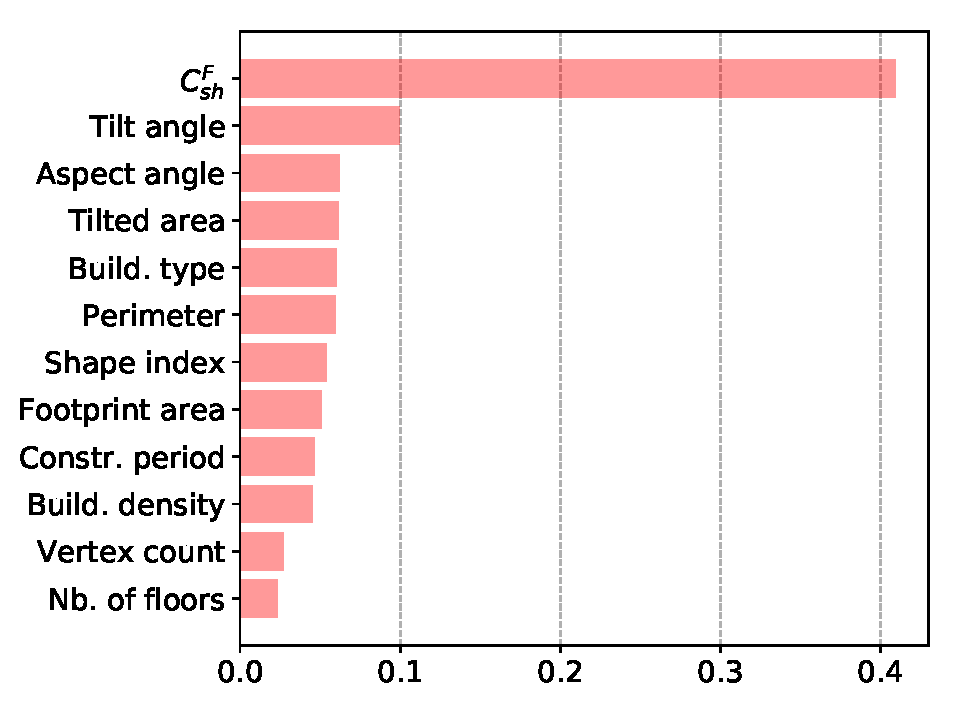
\includegraphics[width=.5\linewidth]{Figs/Feature_importance_shade.pdf}  
\caption{Feature importance of all features considered for the estimation of $C_{sh}$.}
\label{fig:RF_Csh}
\end{figure}

\begin{table}[tb]
\centering
\footnotesize
\caption{Errors for estimating $C_{sh}$. Baseline is the error between $C_{sh}^F$ and $C_{sh}^T$, for MBE+ and RF models.}
\label{tab:errors_Csh}
\begin{tabular}{lcccc}
\hline
      & \textbf{Baseline} & \textbf{MBE+} & \textbf{RF}   \\ \hline
RMSE  & 0.23     & 0.21  & 0.18 \\
MAE   & 0.13     & 0.14  & 0.12 \\
MBE   & 0.09     & 0.00  & 0.00 \\
R$^2$ & 0.12     & 0.25  & 0.44 \\ \hline
\end{tabular}
\end{table}

The sky view factor (SVF), representing the visible proportion of the sky, is computed by combining the vertical elevation angles of the horizon for a discretized set of directions \cite{zaksek_sky-view_2011}. We find 32 equally spaced directions to be sufficient for a precise estimation of the SVF, which we have implemented according to \ref{app:shade}.
Using the DSM$_{2\text{m}}$ and the DSM$_{50\text{cm}}$, we compute a national $\mathit{SVF}^F$ and a "true" $\mathit{SVF}^T$ in Geneva, respectively. The MBE between the two variables is 7.16\%.  
As the error of $\mathit{SVF}^F$ with respect to $\mathit{SVF}^T$ follows no identifiable pattern given the available features, we apply bias-correction (MBE+) to adjust the $\mathit{SVF}^F$ at national scale based on data from the high-resolution DSM$_{50\text{cm}}$, similar to $S_{sh}$ in Section~\ref{shade}.

%%%%%%%%%%%%%%%%%%%%%%%%%%%%%%%%%%%%%%%%%%%%%%

\subsection{Flat rooftops}
\label{flat}

For a more realistic representation of PV panels on flat roofs, we assume PV panels to be installed in individual south-facing rows instead of placing them in consecutive rows along the roof aspect. Some spacing is left between the rows to reduce mutual shading effects between them (see Fig~\ref{fig:panels}).
The tilt angle and row spacing is chosen as a trade-off between the total PV output and the capacity factor, which is a proxy of the economic feasibility.
We have simulated different configurations and found a technically optimal trade-off for a tilt angle of $30^\circ$ and a spacing of one panel height at the Swiss latitude.

The installation strategy on flat roofs impacts the PV potential in multiple ways: (i) tilted radiation increases due to the panel tilt of $30^\circ$, (ii) $C_{\mathit{pv}}$ decreases due to the spacing of the rows, (iii) mutual shading between adjacent rows of panels increases the hourly shaded fraction and (iv) the sky view factor is reduced. The $S_{sh}$ and the $\mathit{SVF}$ of flat roofs are hence multiplied with an additional hourly shading factor ($S_{\mathit{flat}}(t)$) and sky view factor ($\mathit{SVF}_{\mathit{flat}}$), respectively, which we have simulated using the geometric model explained in Appendix~\ref{app_flat}. 

%%%%%%%%%%%%%%%%%%%%%%%%%%%%%%%%%%%%%%%%%%%%%%%%%%%%%%%

\subsection{Uncertainty}
\label{unc}

The technical potential depends on multiple variables, as shown in Fig.~\ref{fig:workflow_PV}. 
The best estimate for each variable is given by their first and second order moments, which may be used to combine various uncertainties using statistical methods.
%
Uncertainties arise from different sources and are unknown in some cases. 
In this work, we consider only those uncertainties for which information can be extracted from the statistical analysis of our data. Further potential sources of uncertainty will be discussed in Section~\ref{limitations_pv}.

\subsubsection{Uncertainty for ML methods}

To estimate the uncertainties for the output variables of the ML models, namely $G_h, G_B, \rho, C_{sh}$ and $C_{\mathit{pv}}$, we follow the two-stage approach presented in Chapter~\ref{unc_ML}. 
It distinguishes between the uncertainty arising from the modelling process (model uncertainty, $\sigma_M$) and the uncertainty related to the data noise (data uncertainty, $\sigma_D$) \cite{wan_probabilistic_2014}. 
The data uncertainty may also represent errors introduced by previous processing steps, for example using GIS. 

The model uncertainty is estimated as the standard deviation of the predictions from each ensemble member of the RF or ELM-E \cite{heskes_practical_1997, wan_probabilistic_2014}. 
To quantify the data uncertainty, a second ML model is trained on the remaining residuals of the out-of-bag training data~\cite{breiman_bagging_1996}, which are derived from the squared difference between the targets and predictions~\cite{heskes_practical_1997, wan_probabilistic_2014}. This second ML model is used to predict $\sigma_D$ for each predicted output (see Chapter~\ref{unc_ML} for details). In this work, we use the same hyper-parameters for the residual model as we use for the respective primary ML model (i.e. $G_h, G_B, \rho, C_{sh}$ and $C_{\mathit{pv}}$), reported in Appendix \ref{app:tuning}.
% Further information regarding our implementation of this method is provided in Chapter~\ref{unc_ML}.
The total uncertainty of a variable estimated using ML is then the squared sum of its model uncertainty and its data uncertainty.

% SOURCE: ELM PAPER
\begin{comment}
The observed spread represents the intrinsic data uncertainty which we measure using the residuals. For modelling these residuals, an analysis equivalent to the one presented above is conducted, giving optimal model hyper-parameters of L = 500 and M = 50.
\end{comment}

\subsubsection{Uncertainty for GIS methods}

The uncertainty for the GIS-derived and bias corrected quantities ($S_{sh}$ and $\mathit{SVF}$) is estimated from the residuals between the values computed using the national DSM$_{2\text{m}}$ ($S_{sh}^F$, $\mathit{SVF}^F$) and the "true" values extracted from the DSM$_{50\text{cm}}$ ($S_{sh}^T$, $\mathit{SVF}^T$) in Geneva.
The error is treated as a random variable, whose first and second moments are computed as the mean and the variance of these residuals. The mean is used for the bias correction, as explained in Sections \ref{shade} and \ref{svf}, while the variance represents the uncertainty.

\subsubsection{Uncertainty propagation}
\label{unc_prop}

The propagation of uncertainty is performed by treating Eqs.~(\ref{eq:Gh})-(\ref{eq:pv}) as functions of randomly distributed variables with statistical errors. 
To compute the variances of their output variables from a combination of the means, variances and covariances of their inputs (summarized in Table~\ref{tab:vars}), we make the following assumptions:
First, statistical independence is assumed between the solar radiation ($G_{h, B, D}$) and the DSM-derived variables ($S_{sh}, \mathit{SVF}$). 
This is valid as the uncertainty of $G_{h, B, D}$ is dominated by the meteorological variability, while that of $S_{sh}(t)$ and $\mathit{SVF}$ is related to errors in the GIS methods. These are independent and uncorrelated processes. 
By contrast, $G_h$ and $G_B$, as well as $S_{sh}$ and $\mathit{SVF}$, exhibit a mutual correlation, as Table~\ref{tab:covrr} shows. Therefore, their covariances must be considered in the uncertainty propagation. 
Second, we assume that $G_t$ and $A_{PV}$, and $C_{\mathit{pv}}$ and $C_{sh}$, are independent as their correlation coefficients are negligible (see Table~\ref{tab:covrr}).
Third, we neglect the uncertainties of $\rho$ and of the temperature data, as these have a low impact on the final results.
Fourth, we do not account for the uncertainty related to the physical models of $G_{Dt}$, $\eta_{PV}$ and $\mathit{PF}$ (Chapter~\ref{phys_models}), due to a lack of data on their performance and the expected errors. This limitation will be discussed in Section \ref{limitations_pv}.

\begin{table}[tb]
\centering
\footnotesize
\caption{Linear correlation coefficients for pairs of potentially correlated random variables. $^1$ denotes a spatio-temporal mean, $^2$ indicates a mean across all time steps $t$.}
\label{tab:covrr}
\begin{tabular}{lc}
    \hline
                        & \textbf{Correlation}  \\ \hline
    $G_h$, $G_B$ $^1$    & 0.87                  \\
    $S_{sh}$, $\mathit{SVF}$ $^2$  & 0.36                  \\ 
    $G_t$, $A_{PV}$ $^2$  & 0.04                  \\
    $C_{\mathit{pv}}$, $C_{sh}$    & 0.02                  \\   \hline 
\end{tabular}
\end{table}

\begin{table}[tb]
\centering
\footnotesize
\caption{Summary of the uncertainties for each variable in the RPV potential estimation. The dimension (dim) of the uncertainties refers to $R$ as roof surfaces and $t$ as time steps.}
\label{tab:uncs}
\begin{tabular} {lcccccccc}
\hline 
\textit{Variable}  & $G_{h,B,D}$  & $S_{sh}$  & $\mathit{SVF}$ & $C_{sh}$ & $C_{\mathit{pv}}$ & $G_t$  & $A_{PV}$ & $E_{PV}$                  \\
\hline 
Uncertainty    & $\sigma_{Gh,B,D}$    & $\sigma_{\mathit{Ssh}}$     & $\sigma_{\mathit{SVF}}$     & $\sigma_{\mathit{Csh}}$  & $\sigma_{\mathit{Cpv}}$    & $\sigma_{Gt}$   & $\sigma_{A}$     & $\sigma_{PV}$                     \\
Dim. of $\sigma$ & $R \times t$ & $t$ & $1$   & $R$     & $R$     & $R \times t$ & $R$    & $R \times t$ \\
\hline 
\end{tabular}
\end{table}

Table~\ref{tab:uncs} summarizes all variables for which uncertainties are considered, as well as the dimensions along which these are derived.
Based on the above assumptions and given the uncertainties in Table~\ref{tab:uncs}, the variances of $G_D$ ($\sigma^2_{GD}$) and $G_t$ ($\sigma^2_{Gt}$) are derived from Eqs.~(\ref{eq:Gh}) and (\ref{eq:irrad}) using the error propagation theory summarized in Chapter~\ref{method_unc_prop}, such that:

\begin{equation}
\label{eq:unc_GD}
\sigma^2_{GD} = \sigma^2_{Gh} +  \sigma^2_{GB} - 2 \mathrm{Cov}(G_h, G_B) 
\end{equation}
%
\begin{equation}
\label{eq:irrad_unc}
\sigma^2_{Gt} = \sigma^2_{B} +  \sigma^2_{D} +  \sigma^2_{R} + 2 (\mathrm{Cov}(B, D) + \mathrm{Cov}(B, R) + \mathrm{Cov}(D, R))
\end{equation}

where the direct, diffuse and reflected components of $G_t$ are denoted as $B=(1 - S_{sh}) * G_{Bt}$, $D=\mathit{SVF} * G_{Dt}$ and $R=G_{Rt}$. The expressions for their variances ($\sigma^2_{B}, \sigma^2_{D}, \sigma^2_{R}$) and covariances are provided in \ref{unc_Gt}. 

The variances of $A_{PV}$ ($\sigma^2_A$) and $E_{PV}$ ($\sigma^2_{PV}$) are derived from Eqs.~(\ref{eq:area}) and (\ref{eq:pv}), respectively:

\begin{equation}
\label{eq:area_unc}
% Definition of variance of diffuse component     
\sigma^2_{A}  = A_{t}^2 (\sigma^2_{\mathit{Csh}} C_{\mathit{pv}}^2 + \sigma^2_{\mathit{Cpv}} (1-C_{sh})^2 + \sigma^2_{\mathit{Csh}} \sigma^2_{\mathit{Cpv}}) 
\end{equation}
%
\begin{equation}
\label{eq:pv_unc}
% Definition of variance of diffuse component     
\sigma^2_{PV}  = \eta_{PV}^2 \mathit{PF}^2 (\sigma^2_{A} G_{t}^2 + \sigma^2_{Gt} A_{PV}^2 + \sigma^2_{Gt} \sigma^2_{A}) 
\end{equation}

%%%%%%%%%%%%%%%%%%%%%%%%%%%%%%%%%%%%%%%%%%%%%%%%%%%%%%%
%%%%%%%%%%%%%%%%%%%%%%%%%%%%%%%%%%%%%%%%%%%%%%%%%%%%%%%

\begin{comment}

\subsection{Prediction and uncertainties}

After defining the model parameters and training the model on the satellite data, we predict the monthly-mean-hourly GHI on a dense grid over Switzerland and estimate the model uncertainty from the ELM ensemble variance and the data uncertainty from the second ELM ensemble trained on the remaining residuals. Table 2 shows the monthly mean predictions and satellite data, as well as model and data uncertainty. All values were summed over the respective time span (month or year) and averaged across all locations. We observe that the predicted monthly mean values are slightly above the satellite data. However, the total difference amounts to 0.2\% of yearly predicted GHI, which is negligible compared to the yearly model uncertainty of 0.94\% of GHI. Overall, data uncertainty dominates with a total of 14.45\% of GHI. Figure 4 shows the high-resolution spatial prediction and the spatial distribution of the uncertainties, summed to yearly values. Note that the scale for the prediction is equivalent to Fig. 2(a). The spatial patterns follow the ones observed in the satellite data, but with much higher precision. In the low-altitude regions of Switzerland, spanning from the west to the north-east of the country, the total potential is low, and so is the model uncertainty. In the high-altitude regions of the Swiss alps with high predicted irradiance, as well as near the borders we can observe a higher model uncertainty, with some peaks at the summits of high mountains. These peaks may be due to spatial extrapolation and a lack of data at these altitudes, as the satellite data is the mean over a pixel. The data uncertainty shows some correlation with the altitude profile of Switzerland and is largest in the south-western part of the country. This can be an indication that the weather in this region is least predictable.
% IN PROCESS: Transfer conference paper ICAE
\end{comment}

\section{Results}
\label{solar_results}

\subsection{Physical potential estimation}
\label{phys}

\begin{table}[b]
\centering
\footnotesize
\caption{Results for the estimation of $G_h$, $G_B$ and $G_D$, showing the monthly predicted values (in kWh/m$^2$) and the model ($\sigma_M$) and data ($\sigma_D$) uncertainties (no distinction for $G_D$), as percentage of the monthly radiation.}
\label{tab:G_results}
% \resizebox{\textwidth}{!}{%
\begin{tabular}{lcccccccccccc} % {X[-1,l] X[-1,c] X[-1,c] X[-1,c] X[-1,c] X[-1,c] X[-1,c] X[-1,c] X[-1,c] X[-1,c] X[-1,c] X[-1,c] X[-1,c]}%  
\hline 
      & \textbf{Jan}  & \textbf{Feb}  & \textbf{Mar}   & \textbf{Apr}   & \textbf{May}   & \textbf{Jun}   & \textbf{Jul}   & \textbf{Aug}   & \textbf{Sep}   & \textbf{Oct}  & \textbf{Nov}  & \textbf{Dec}  \\
\hline 
$G_h$ & 44.9 & 66.1 & 114 & 145 & 168 & 180 & 183 & 151 & 115 & 77.1 & 45.5 & 36.6 \\
$\sigma_{M} (\%)\ $ & 1.32 & 1.02 & 1.01  & 1.27  & 1.09  & 1.16  & 1.32  & 1.12  & 1.36  & 1.15 & 0.97 & 1.03 \\
$\sigma_{D} (\%)\ $  & 19.1 & 15.8 & 15.7  & 13.8  & 13.6  & 11.8  & 13.7  & 12.9  & 19.9  & 18.4 & 19.0 & 14.0 \\
\hline 
$G_B$ & 22.1 & 35.2 & 62.3 & 79.6 & 87.6 & 101 & 107 & 89.7 & 68.2 & 43.1 & 23.3 & 17.8 \\
$\sigma_{M} (\%)\ $ & 2.28 & 1.60 & 1.55 & 1.91 & 1.91 & 2.10  & 2.23  & 1.93 & 2.04 & 1.83 & 1.82 & 2.18 \\
$\sigma_{D} (\%)\ $  & 30.1 & 23.1 & 26.8 & 26.2 & 29.2 & 23.2  & 26.0  & 22.5 & 32.9 & 26.3 & 31.8 & 26.2 \\
\hline 
$G_D$ & 22.8 & 30.9 & 51.8 & 65.3 & 80.1 & 79.6 & 75.4 & 60.9 & 47.0 & 34.0 & 22.2 & 18.8 \\
$\sigma_{GD} (\%)$ & 19.0 & 17.0 & 17.3 & 16.1 & 15.8 & 14.6  & 18.3  & 16.7  & 24.7  & 20.9 & 19.3 & 13.5 \\
\hline
$\rho$ & 0.52 & 0.50 & 0.41 & 0.32 & 0.26 & 0.22 & 0.19 & 0.19 & 0.22 & 0.27 & 0.36 & 0.48 \\
\hline
\end{tabular}
% }
\end{table}

\begin{figure}[tb]
\centering
\begin{subfigure}{.49\textwidth}
  \centering
  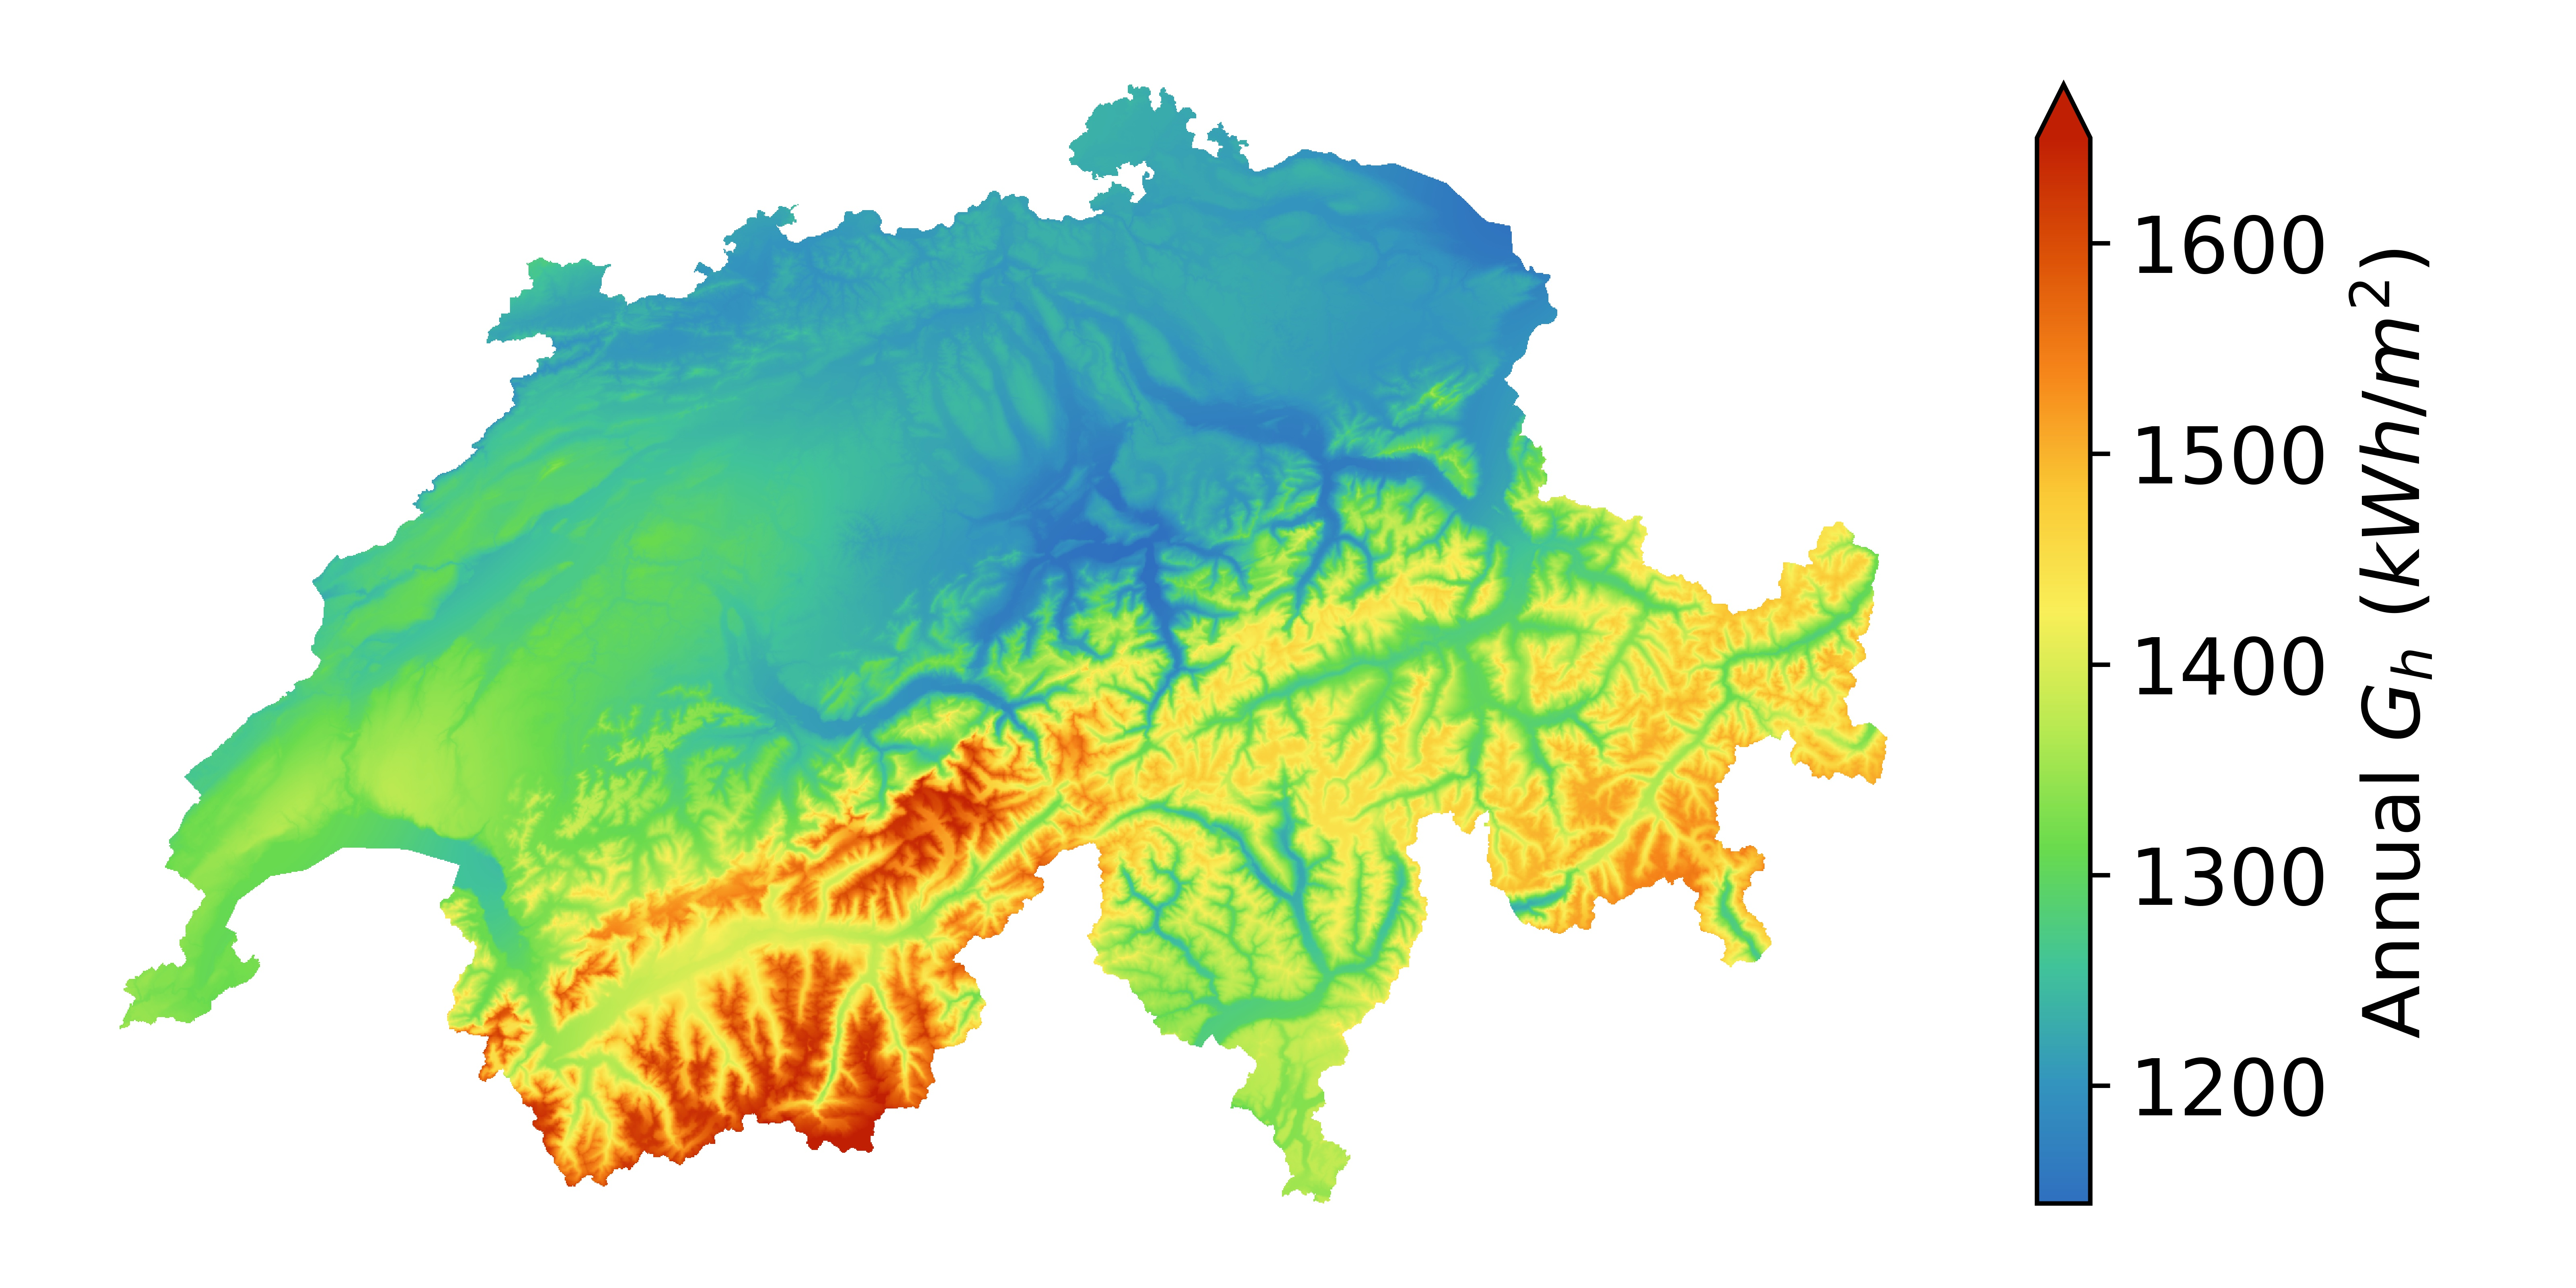
\includegraphics[width=\linewidth]{Figs/SIS_annual.jpg}  
  \subcaption{}
\end{subfigure}
\begin{subfigure}{.49\textwidth}
  \centering
  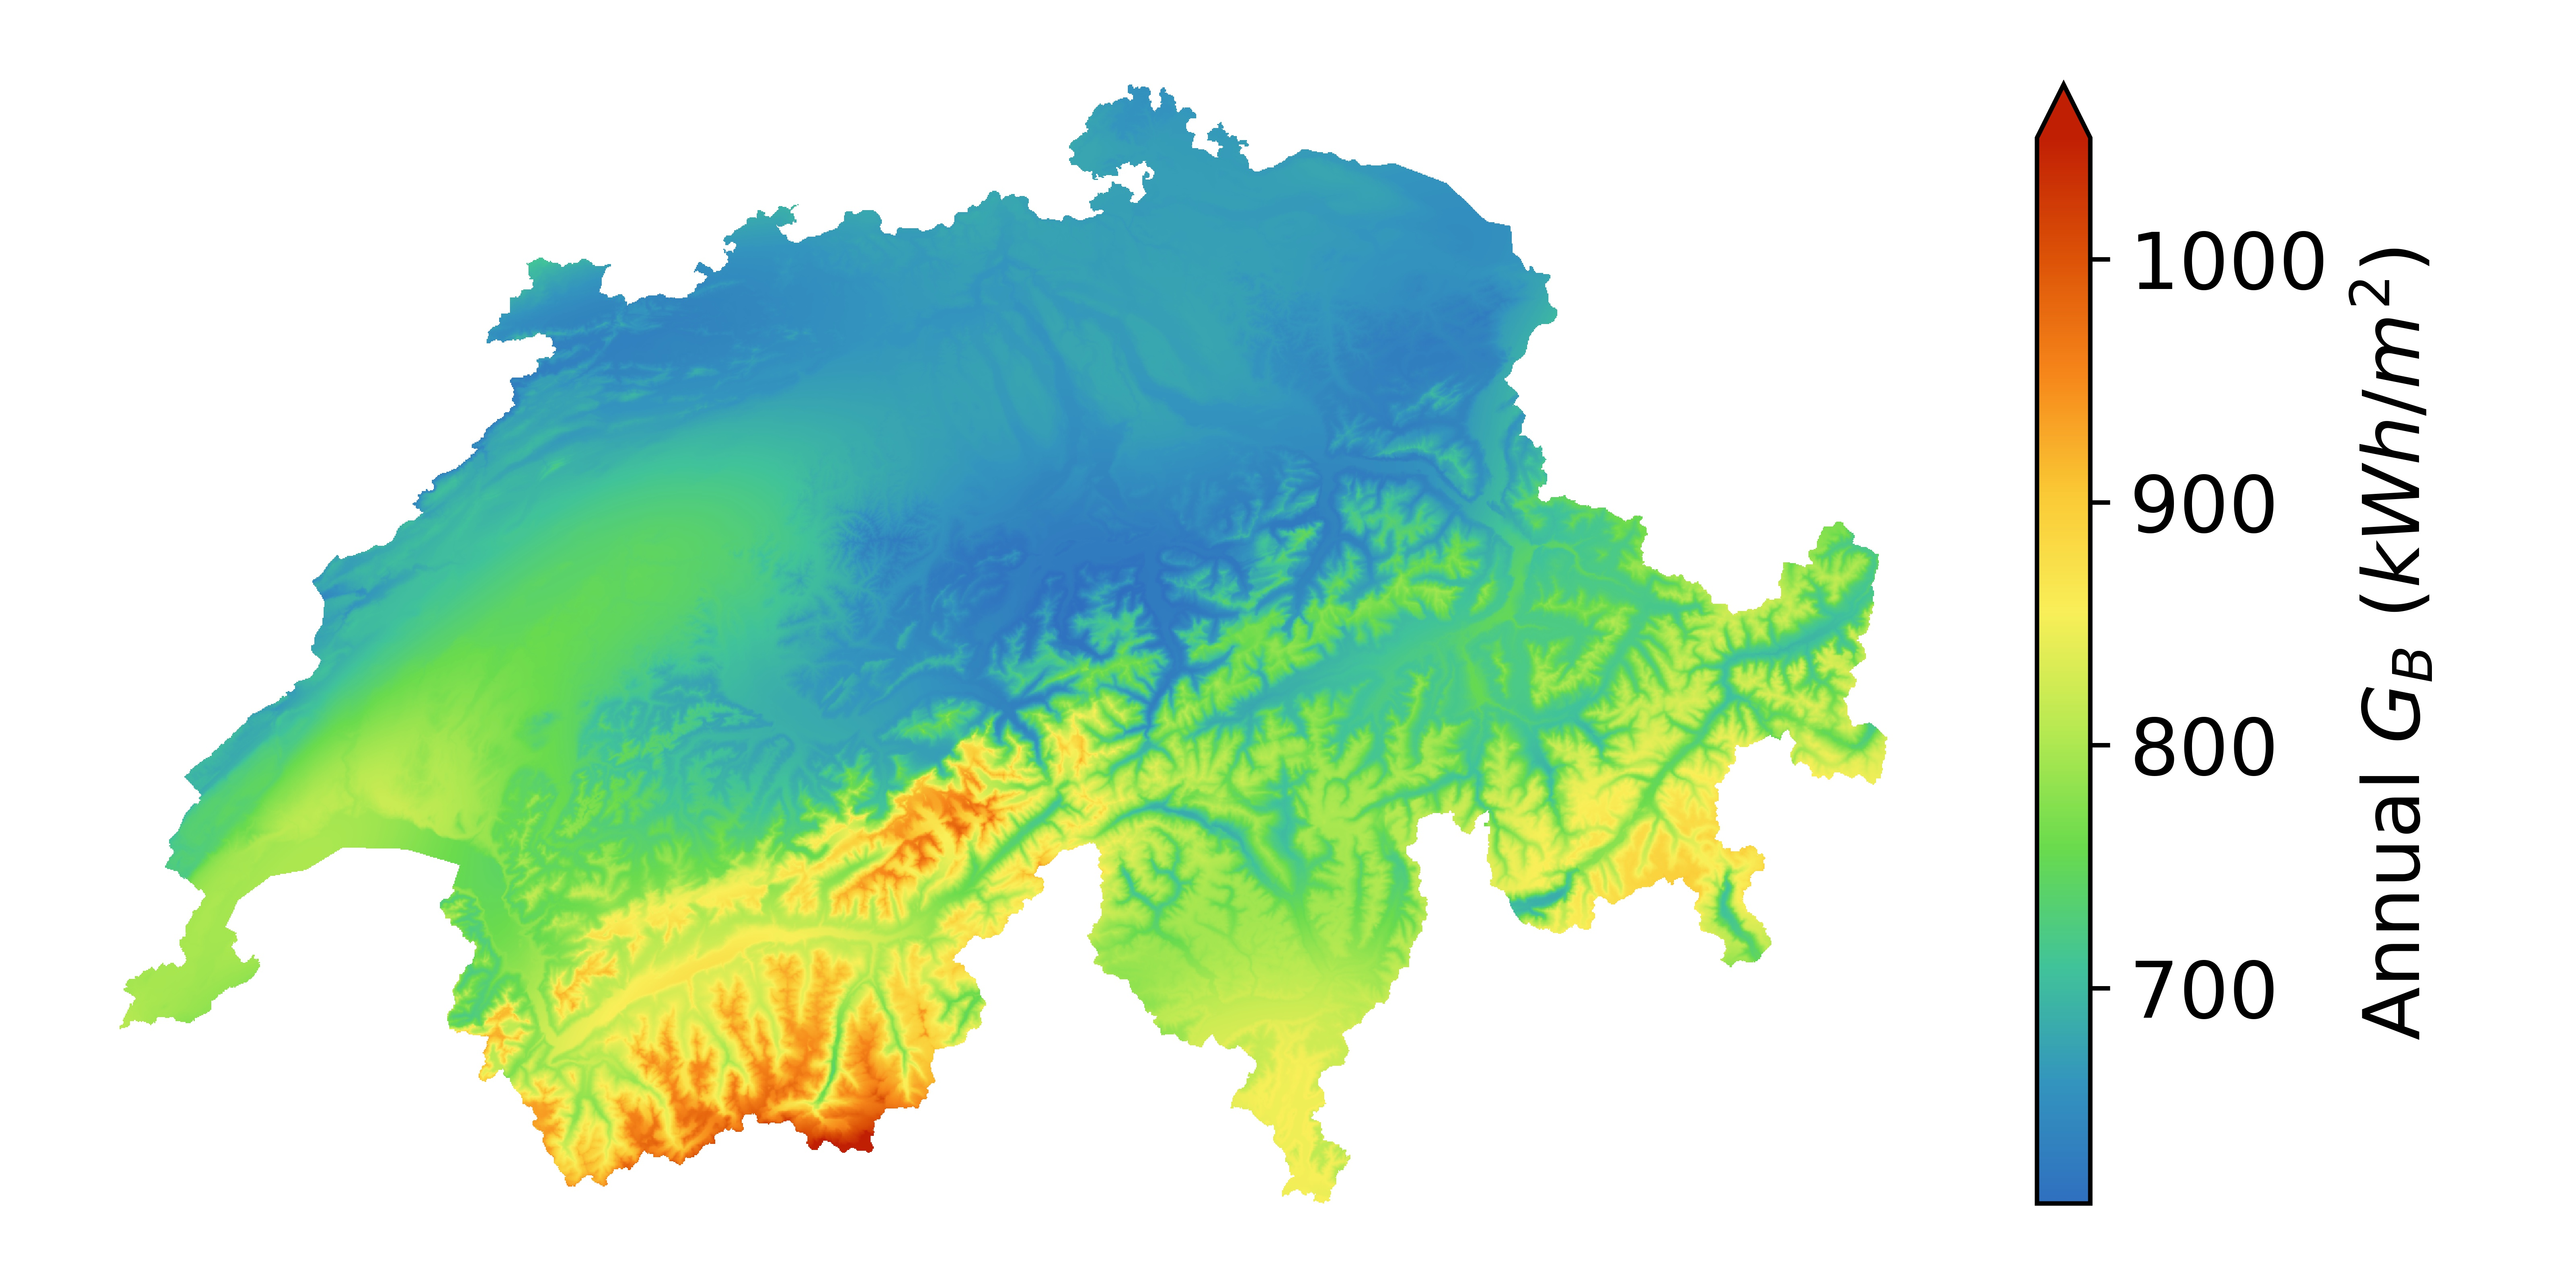
\includegraphics[width=\linewidth]{Figs/SISDIR_annual.jpg}  
  \subcaption{}
\end{subfigure}
\begin{subfigure}{.49\textwidth}
  \centering
  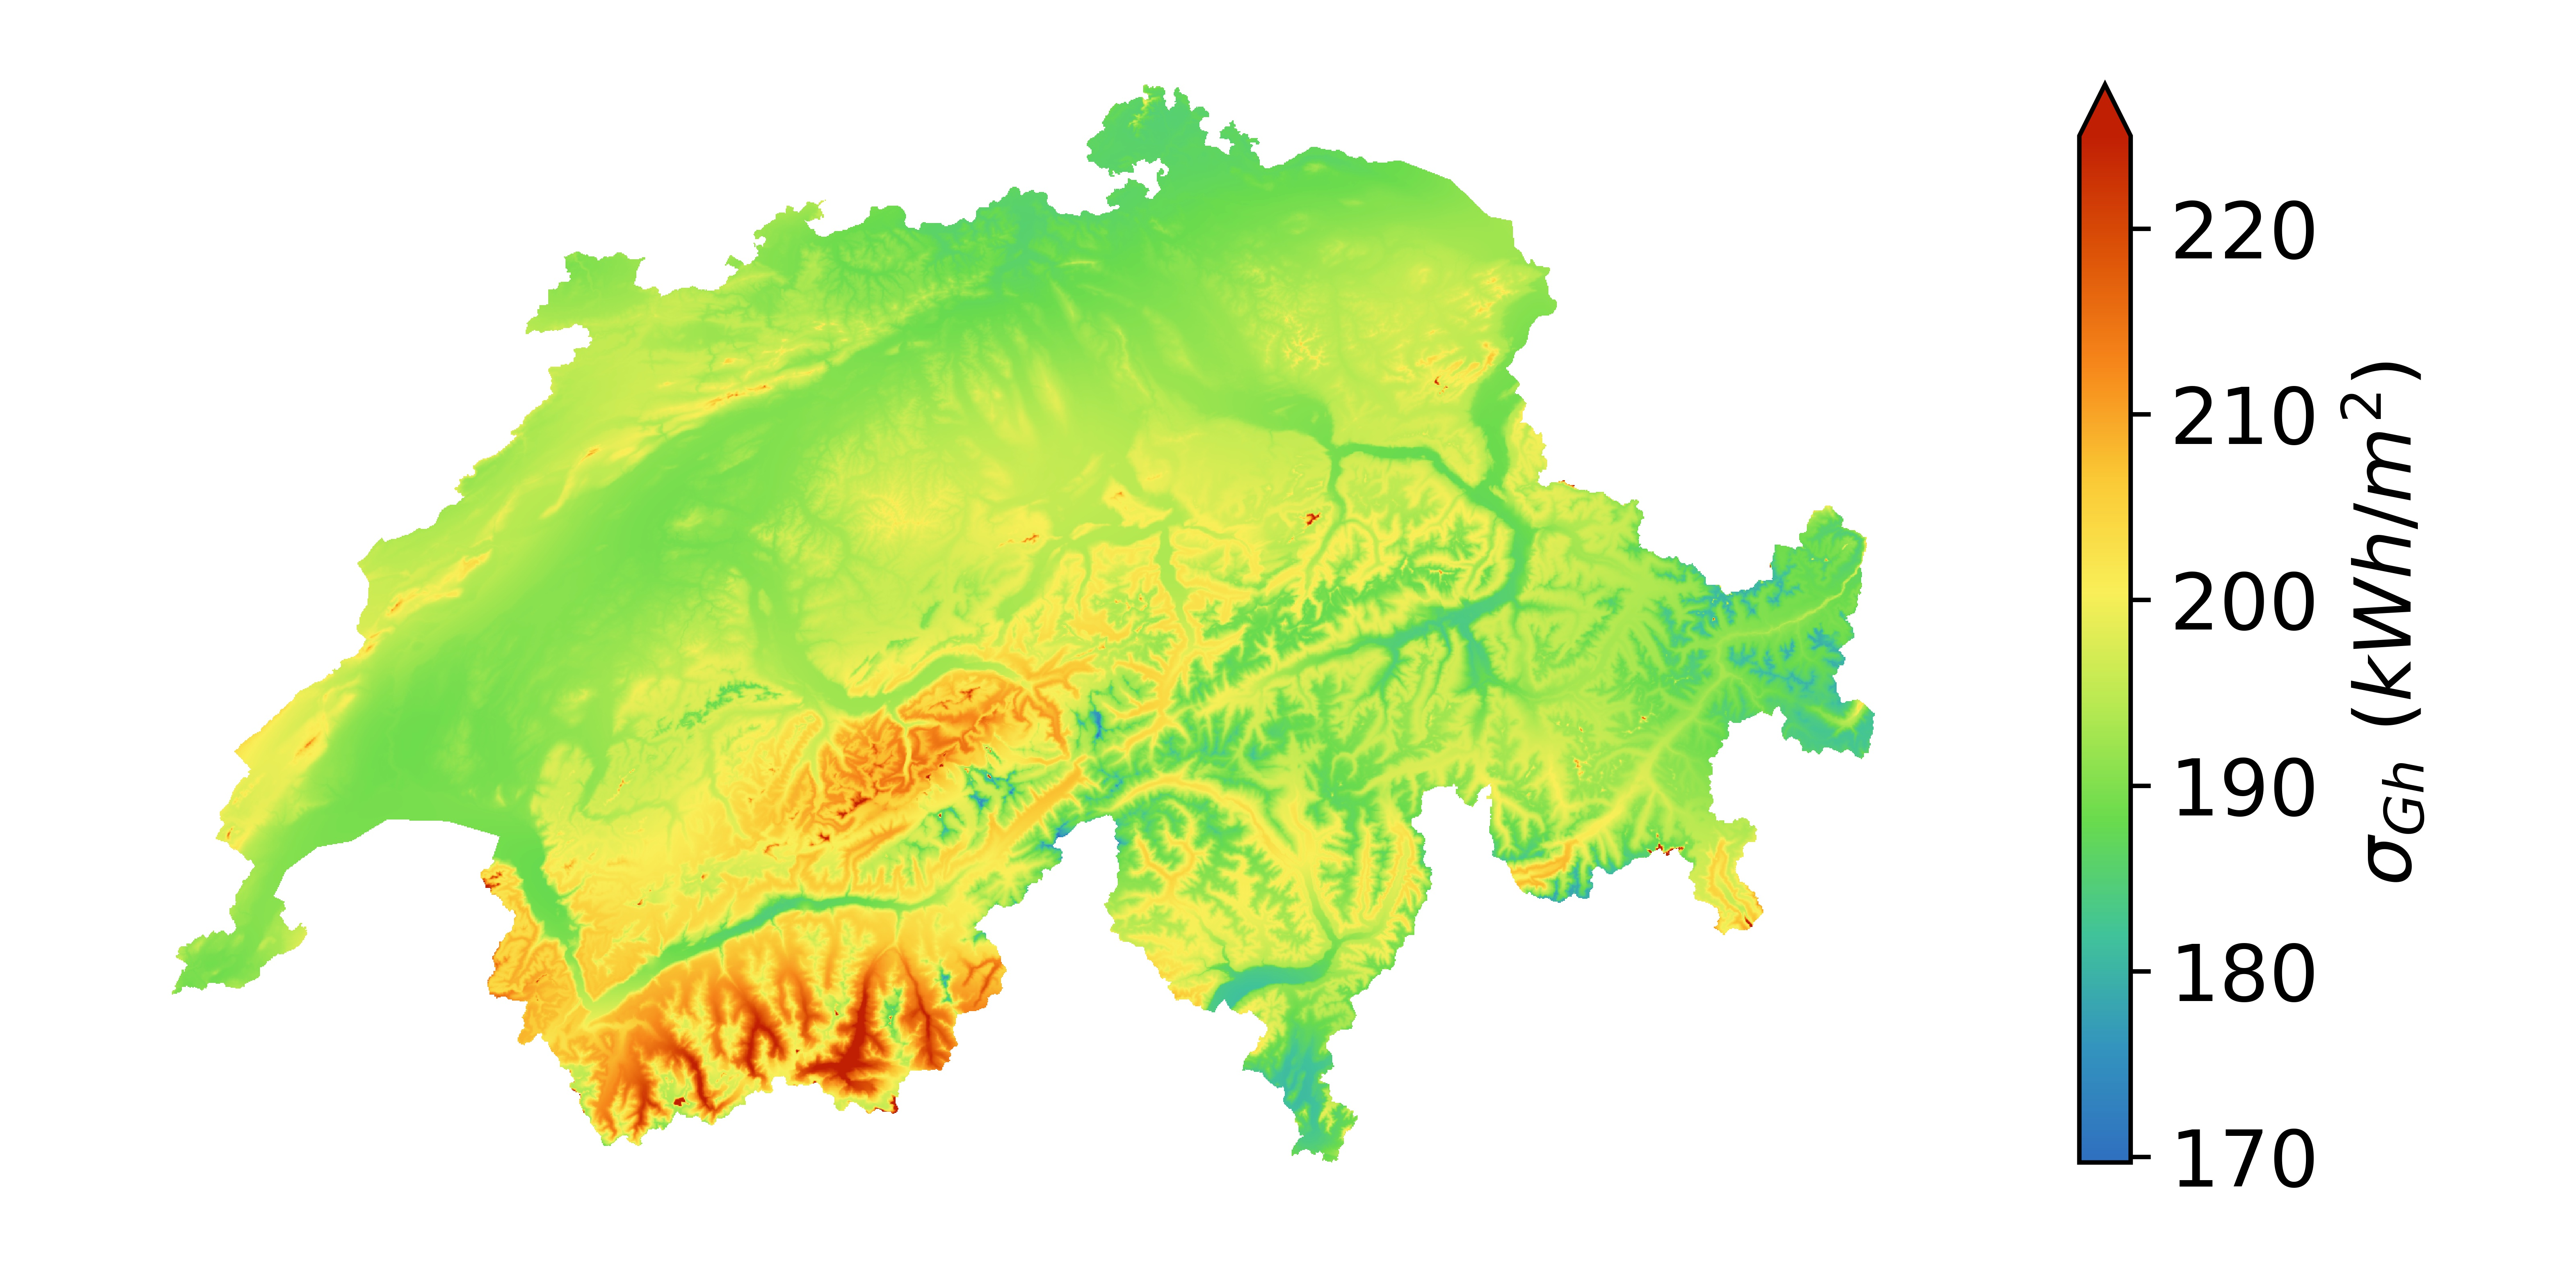
\includegraphics[width=\linewidth]{Figs/SIS_unc_annual.jpg} 
  \subcaption{}
\end{subfigure}
\begin{subfigure}{.49\textwidth}
  \centering
  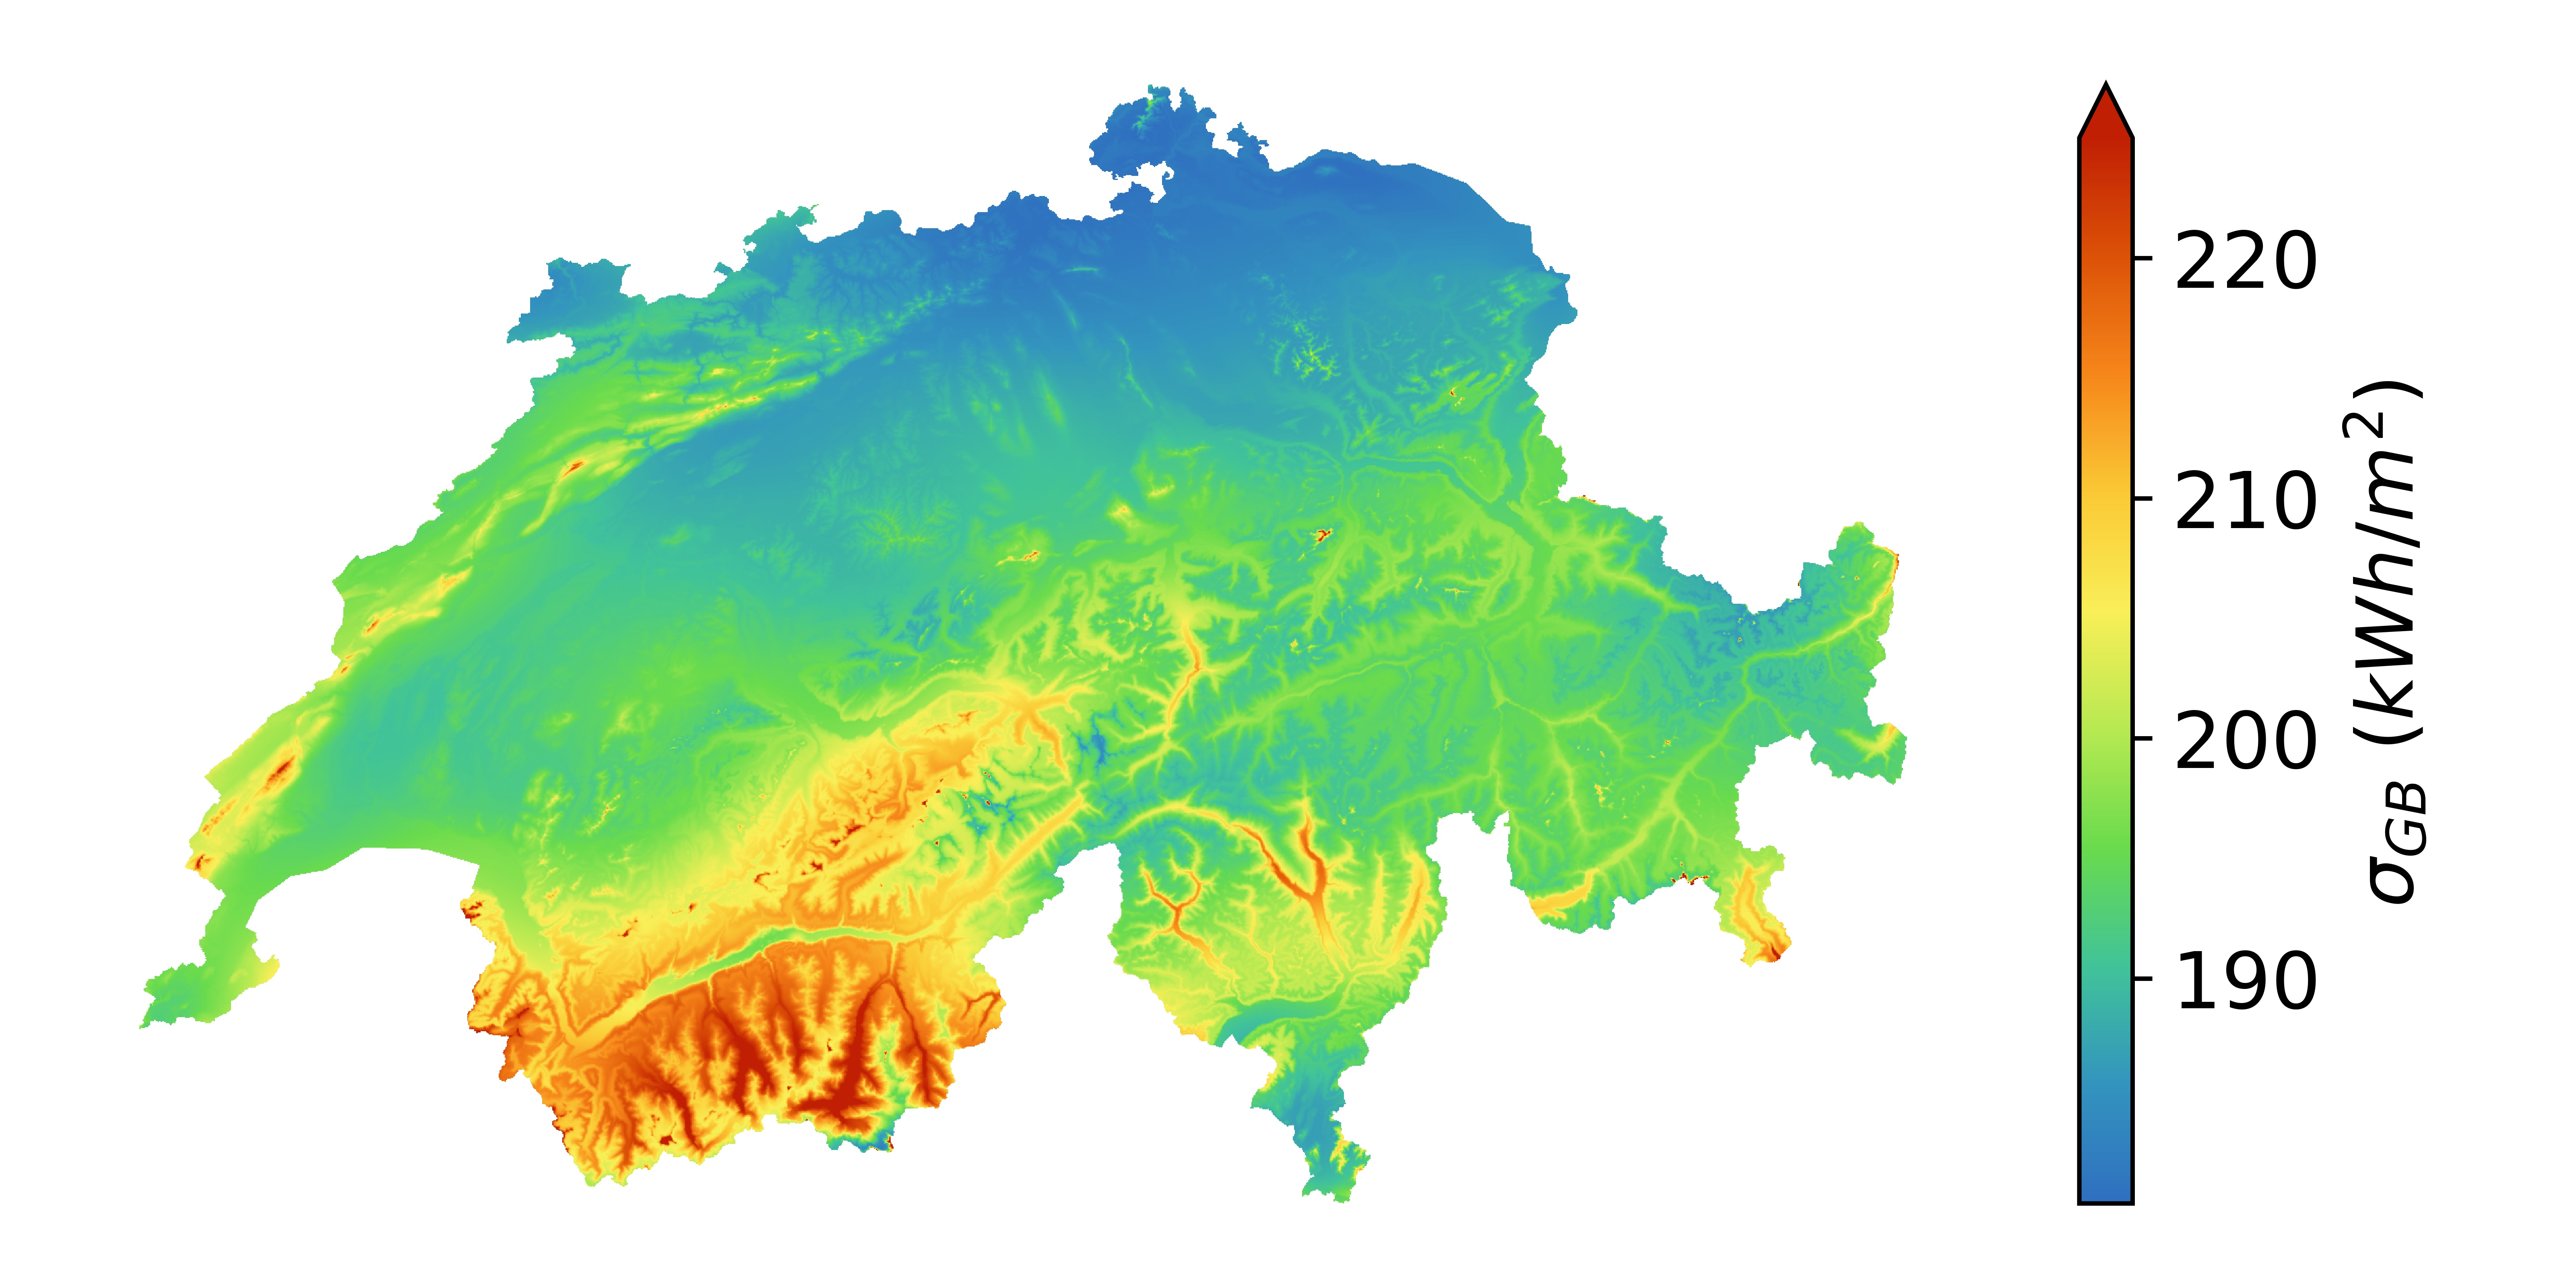
\includegraphics[width=\linewidth]{Figs/SISDIR_unc_annual.jpg}  
  \subcaption{}
\end{subfigure}
\caption{Spatial distribution of annual predicted $G_h$ (a) and $G_B$ (b) for Switzerland, and the total uncertainties $\sigma_{Gh}$ (c) and $\sigma_{GB}$ (d).}
\label{fig:Gh_GB}
\end{figure}

The models of Section~\ref{irrad} are used to predict the MMH solar horizontal radiation and the monthly albedo for each pixel of the $200\times200$ m$^2$ output grid in Switzerland. 
The results, as well as the estimated model and data uncertainties (Section \ref{unc}), are reported in Table~\ref{tab:G_results} as monthly sums, averaged across all pixels. The uncertainty of $\rho$ is not shown as it is neglected in the uncertainty propagation.
For $G_h$ and $G_B$, the model uncertainty $\sigma_M$ is negligible compared to the data uncertainty $\sigma_D$ due to the large amount of training data.
The model performs better for the prediction of $G_h$ than $G_B$. This may be explained by the large relative data uncertainty of $G_B$ (up to 32\%), indicating that its hourly variability is higher than that of $G_h$. 
The results for $\rho$ are close to the standard value of 0.2 in the summer and reach up to 0.5 on average in the winter due to snow coverage at high altitudes in the Swiss alps.

Figure \ref{fig:Gh_GB}a and b show the spatial distribution of $G_h$ and $G_B$ for Switzerland, while Fig. \ref{fig:Gh_GB}c and d show $\sigma_{Gh}$ and $\sigma_{GB}$, which are dominated by the data uncertainty. The highest solar radiation and the largest uncertainty is found at high altitudes in the south of the country where weather extremes are frequent. The majority of buildings are however located at lower altitudes in the Swiss plateau, which spans from the north-west to the north-east of the country. The uncertainty tends to be low here, so the weather patterns are more predictable. In the plateau, also the values for $\rho$ (not shown in Fig.~\ref{fig:Gh_GB}) lie below the averages quoted in Table~\ref{tab:G_results} with a low uncertainty, which shows that $\rho$ mostly impacts the potential at high altitudes.

%%%%%%%%%%%%%%%%%%%%%%%%%%%%%%%%%%%%%%%%%%%%%%%%%%%%%%%

\subsection{Geographic potential estimation}
\label{solar_geo}

%%%%%%%%%%%%% APV %%%%%%%%%%%%%%%%%%%%%%

The available area for PV panel installation ($A_{PV}$) is obtained from the \textit{shaded area coefficient} ($C_{\mathit{pv}}$) and the \textit{panelled area coefficient} ($C_{sh}$) using Eq.~(\ref{eq:area}). Its uncertainty $\sigma_{A}$ is derived from $C_{\mathit{pv}}, C_{sh}$ and their total uncertainties ($\sigma_{\mathit{Cpv}}, \sigma_{\mathit{Csh}}$) using Eq.~(\ref{eq:area_unc}).

\begin{figure}[tb]
\centering
\begin{subfigure}{.49\textwidth}
  \centering
  % include second image
  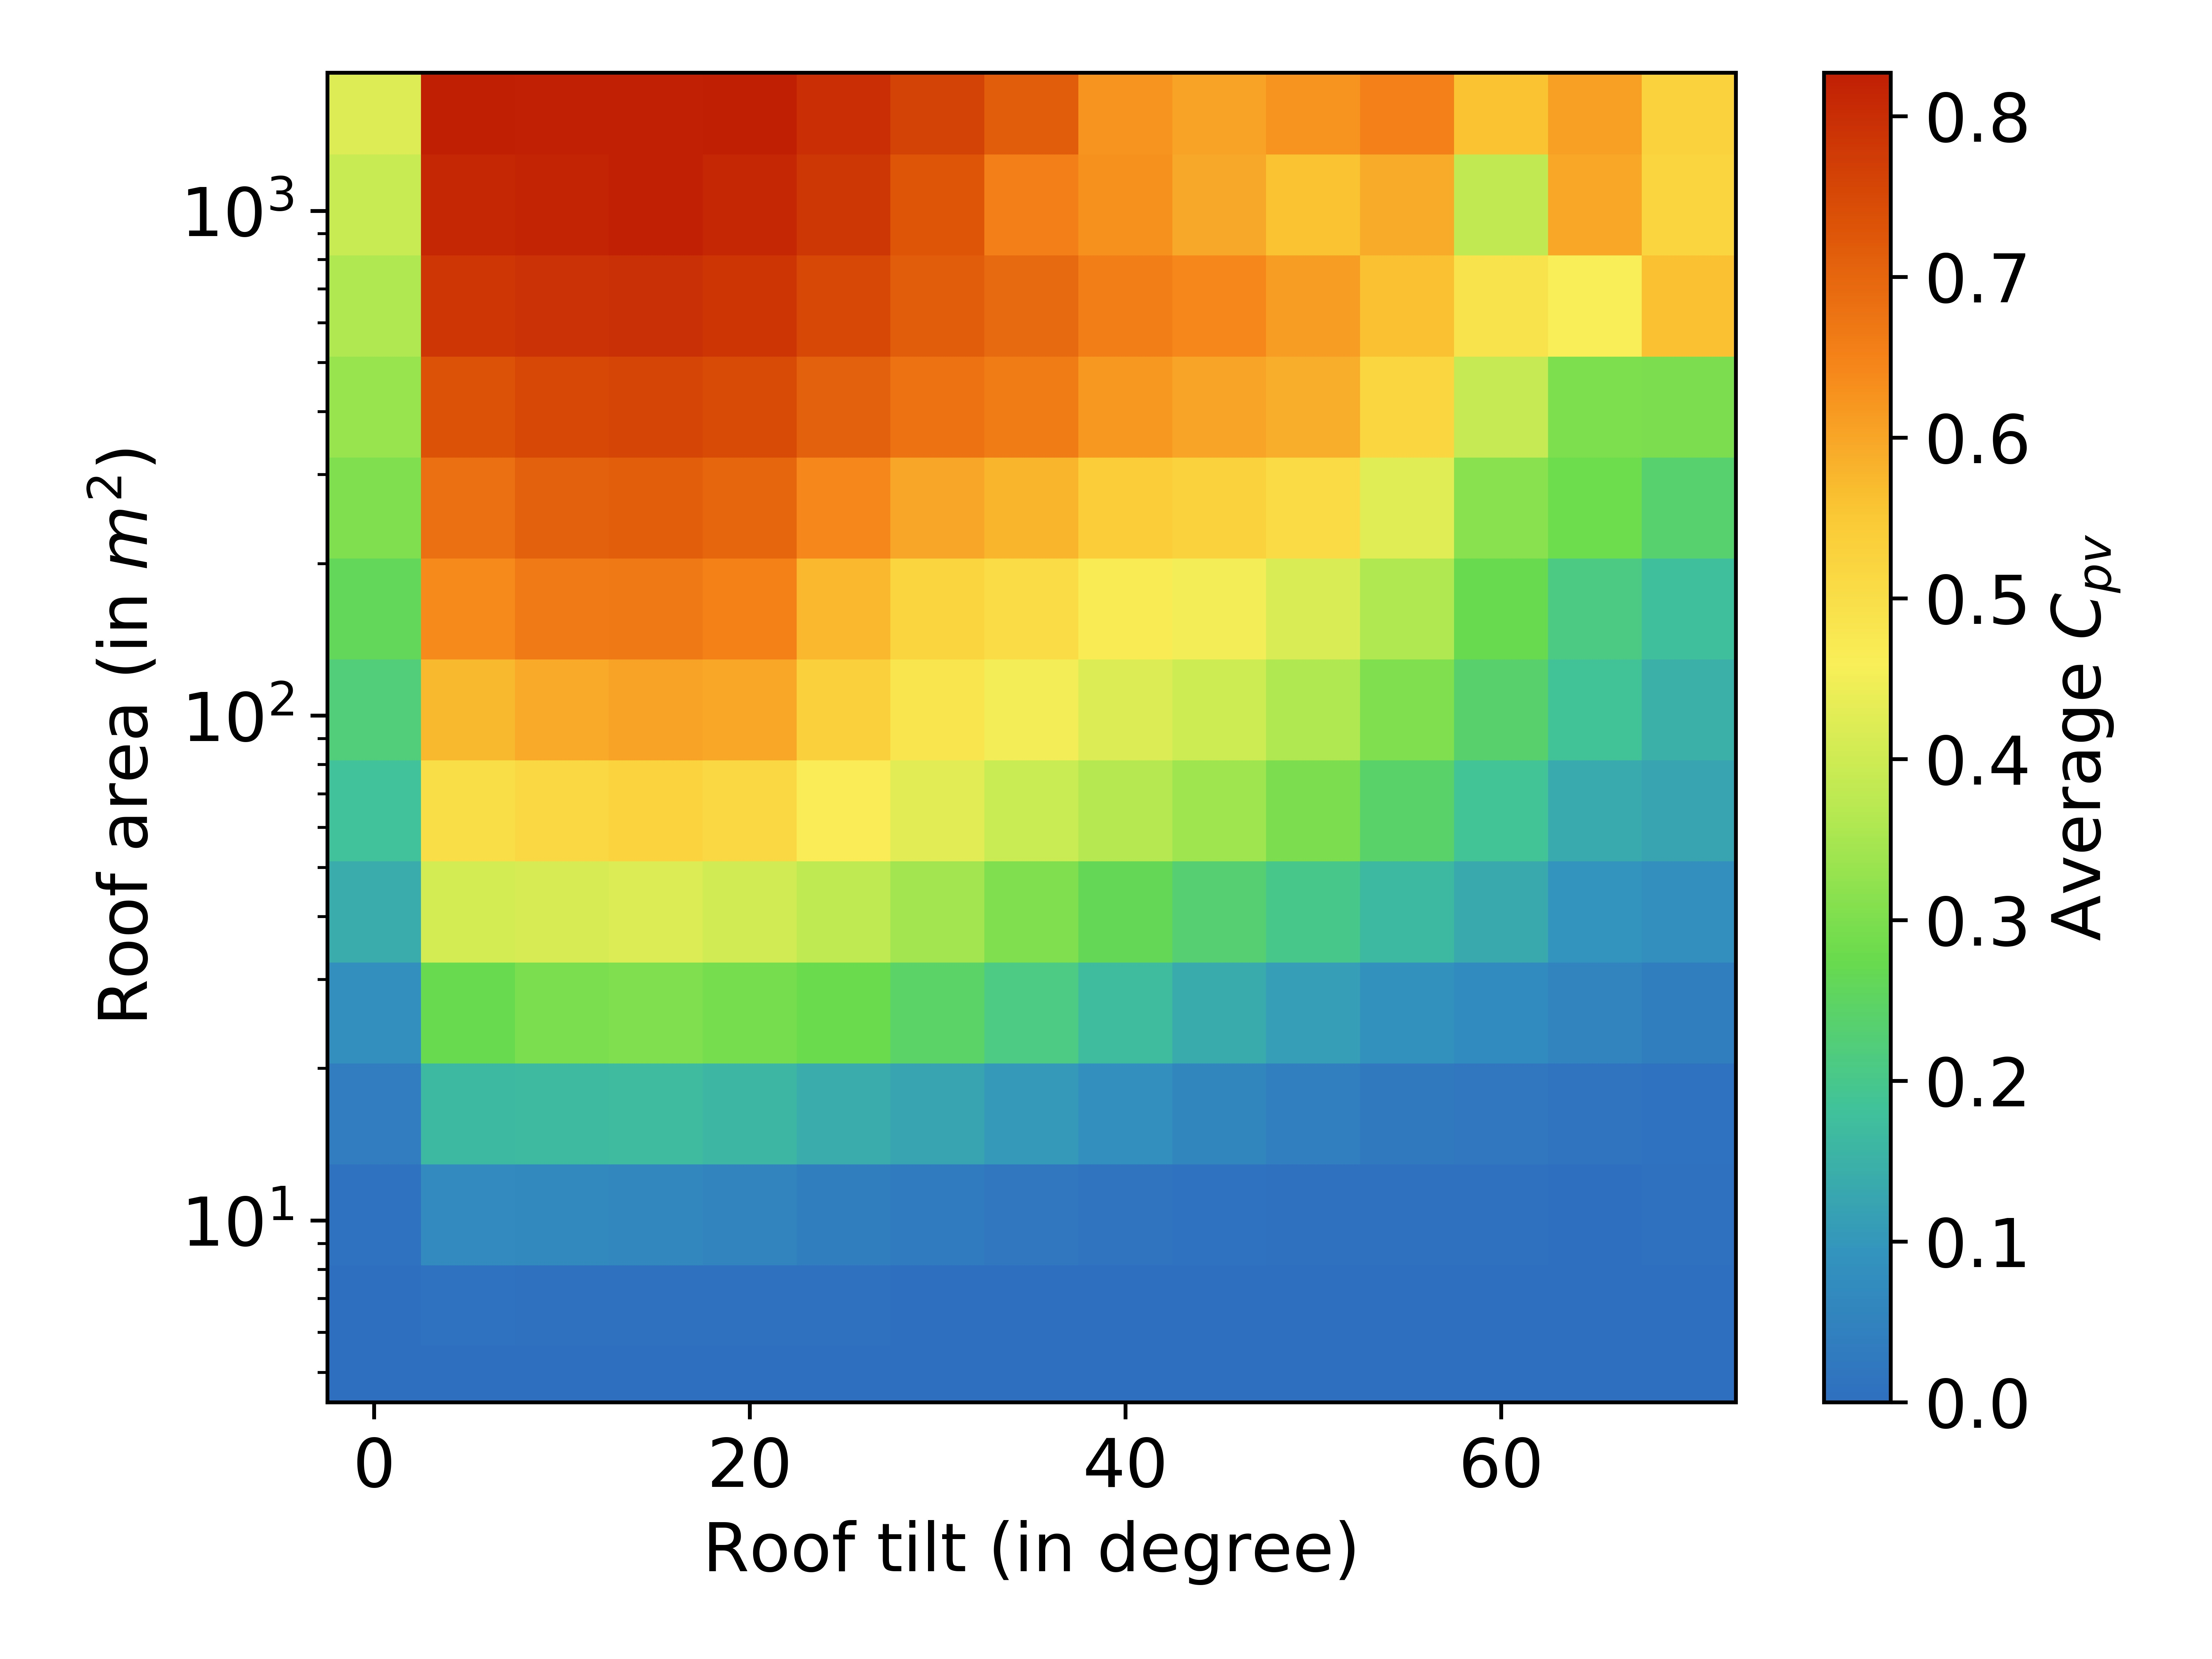
\includegraphics[width=0.9\linewidth]{Figs/panelled_area_ratio.jpg}
  \subcaption{}
\end{subfigure}
\begin{subfigure}{.49\textwidth}
  \centering
  % include first image
  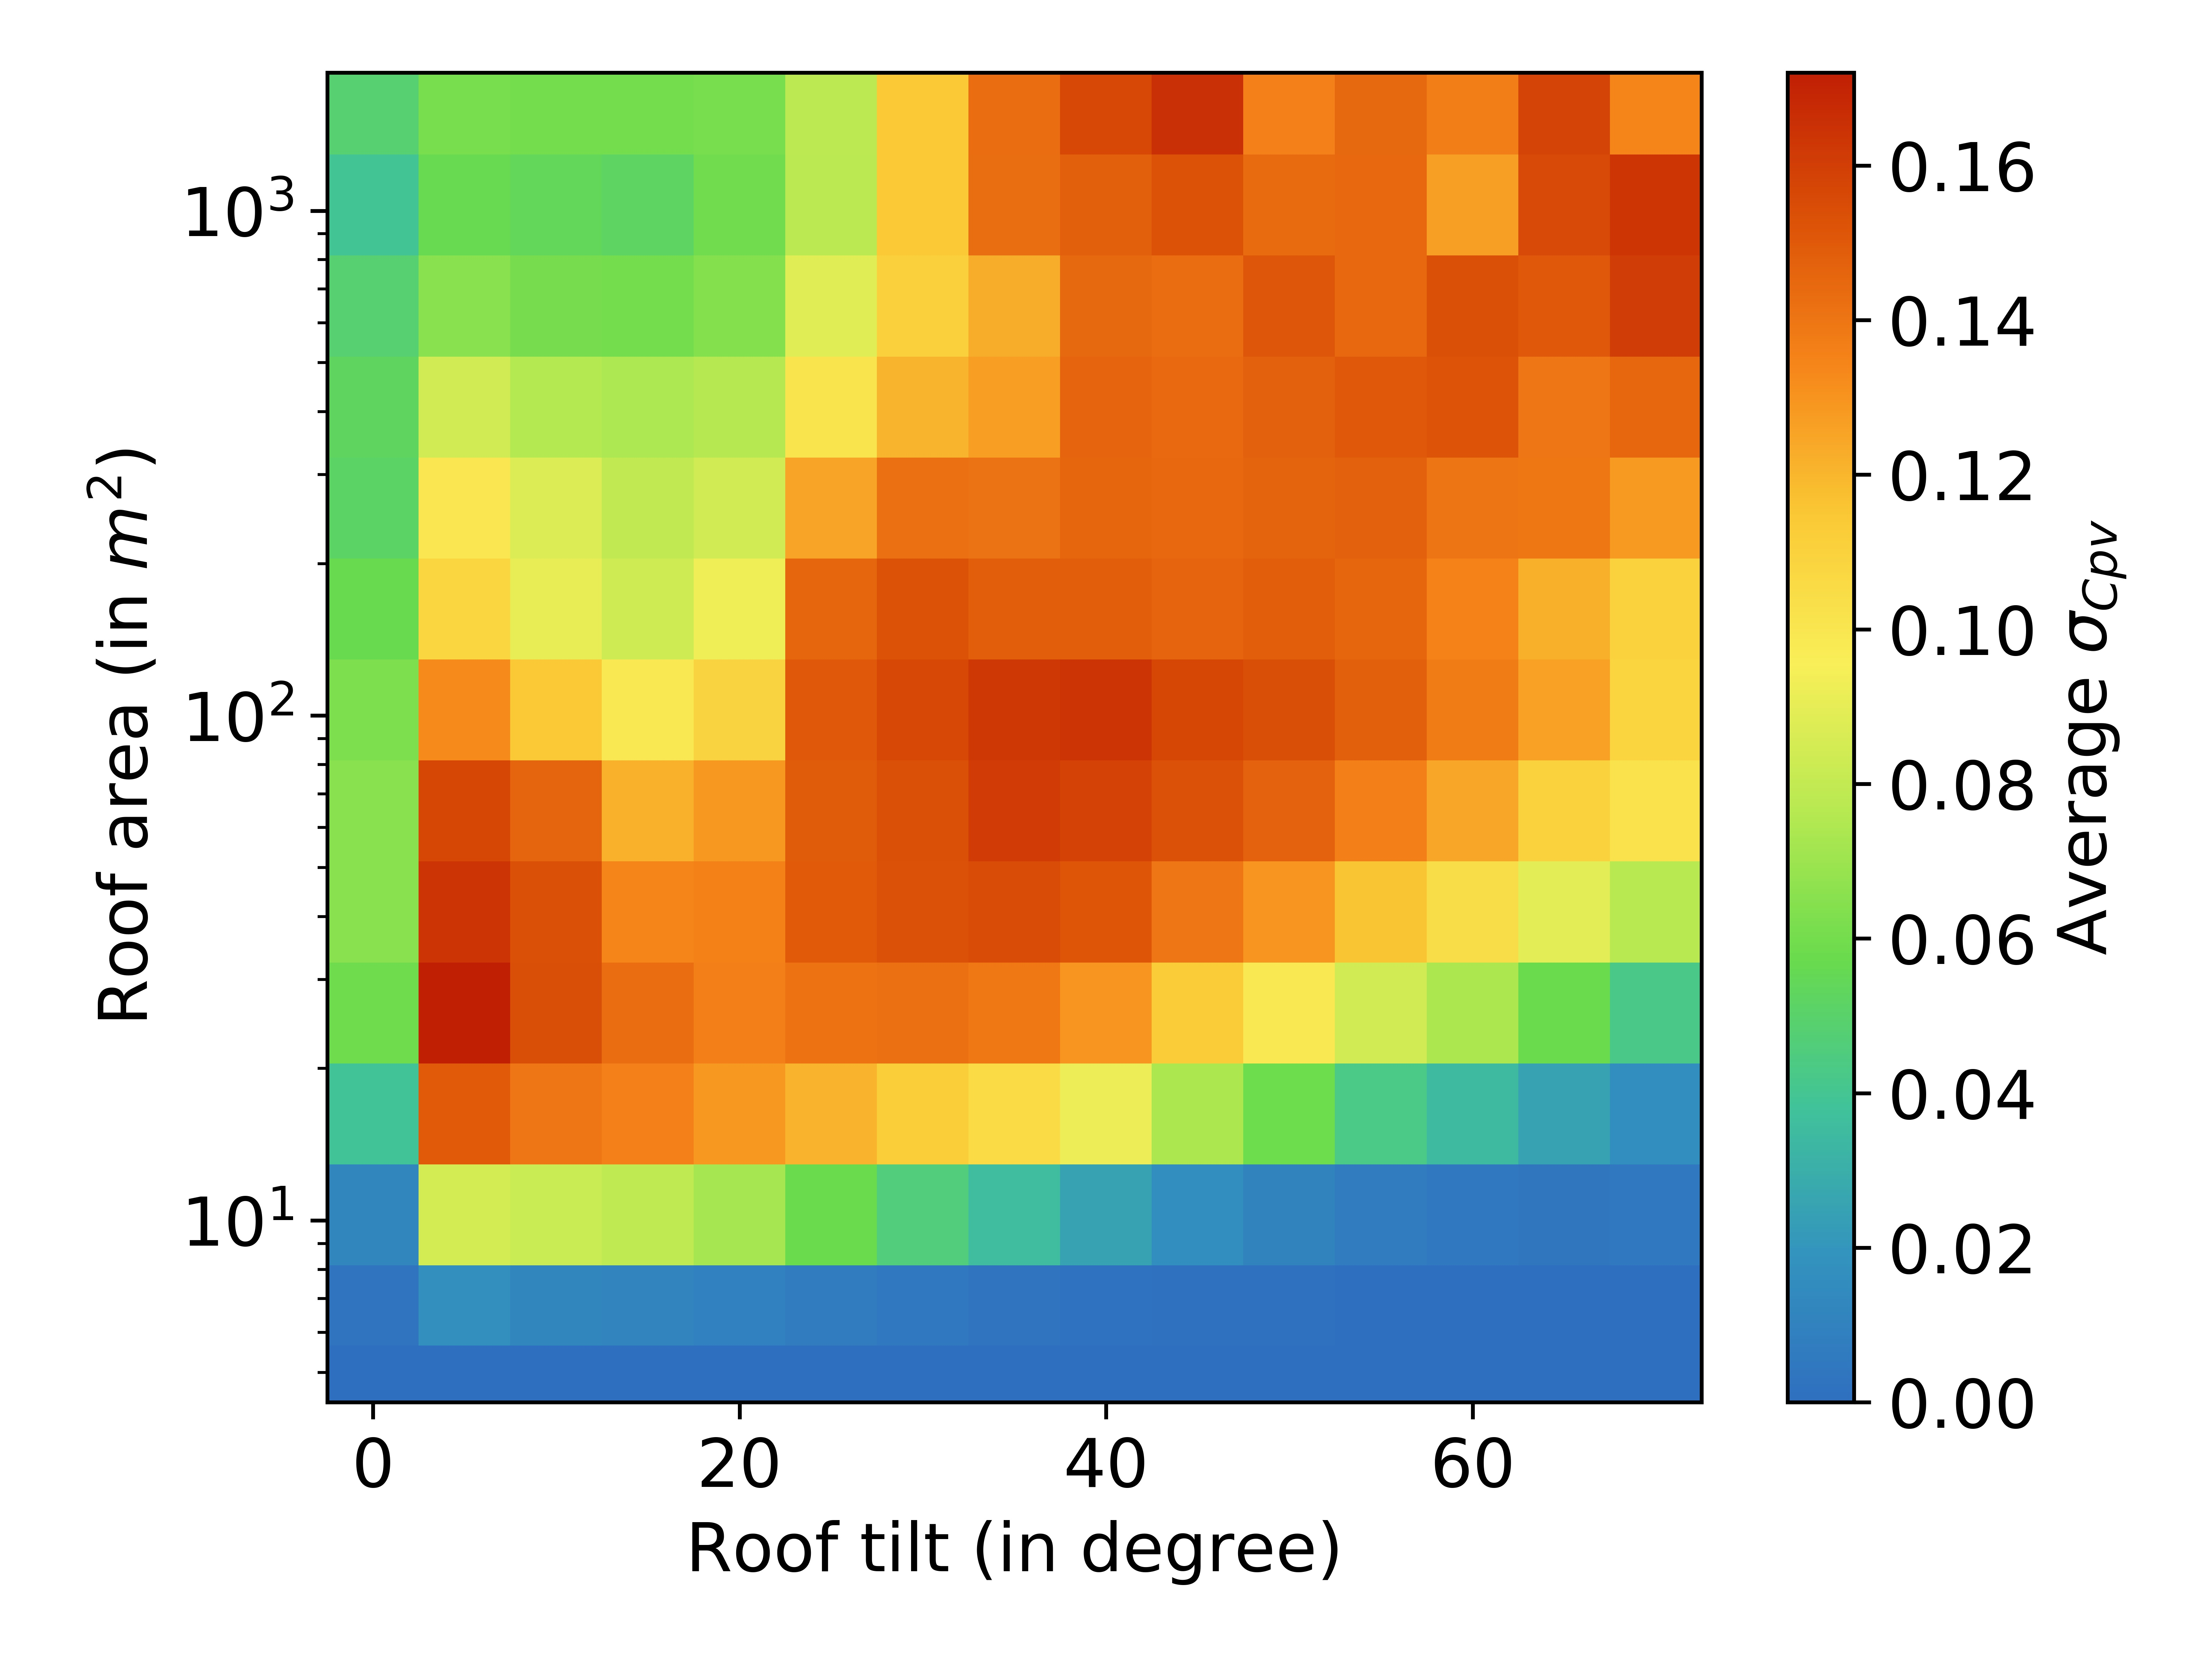
\includegraphics[width=0.9\linewidth]{Figs/panelled_area_unc.jpg}  
  \subcaption{}
\end{subfigure}
\caption{a) Panelled area coefficient $C_{\mathit{pv}}$ and b) associated uncertainty $\sigma_{\mathit{Cpv}}$, per roof tilt and roof area.}
\label{fig:C_pv}
\end{figure}

Figure~\ref{fig:C_pv} shows the final values for $C_{\mathit{pv}}$ (a) and $\sigma_{\mathit{Cpv}}$ (b) as a function of roof tilt and roof area, which is shown on a logarithmic scale. 
Large areas with a low tilt have the highest $C_{\mathit{pv}}$ (70-80\%) and a small uncertainty.
This is due to the high number of installed panels, which reduces the relative effects of the roof shape and the presence of superstructures on $C_{\mathit{pv}}$. Large roofs with a steep tilt have a high uncertainty, as they are rare.
Due to the panel placement strategy for flat roofs (see Section~\ref{flat}), these tend to have a lower $C_{\mathit{pv}}$. 
The highest uncertainty appears for medium-sized roofs (10-100 m$^2$) with $C_{\mathit{pv}}$ in the range of 0.3-0.6. In this range, exact roof shapes as well as the favourable or unfavourable location of superstructures may change the number of installed panels considerably.
Very small areas ($< 10$ m$^2$) have nearly zero available area and a low uncertainty, as the roof shape is frequently unsuitable for the installation of the rectangular panels.

\begin{figure}[tb]
\centering
\begin{subfigure}{.49\textwidth}
  \centering
  % include second image
  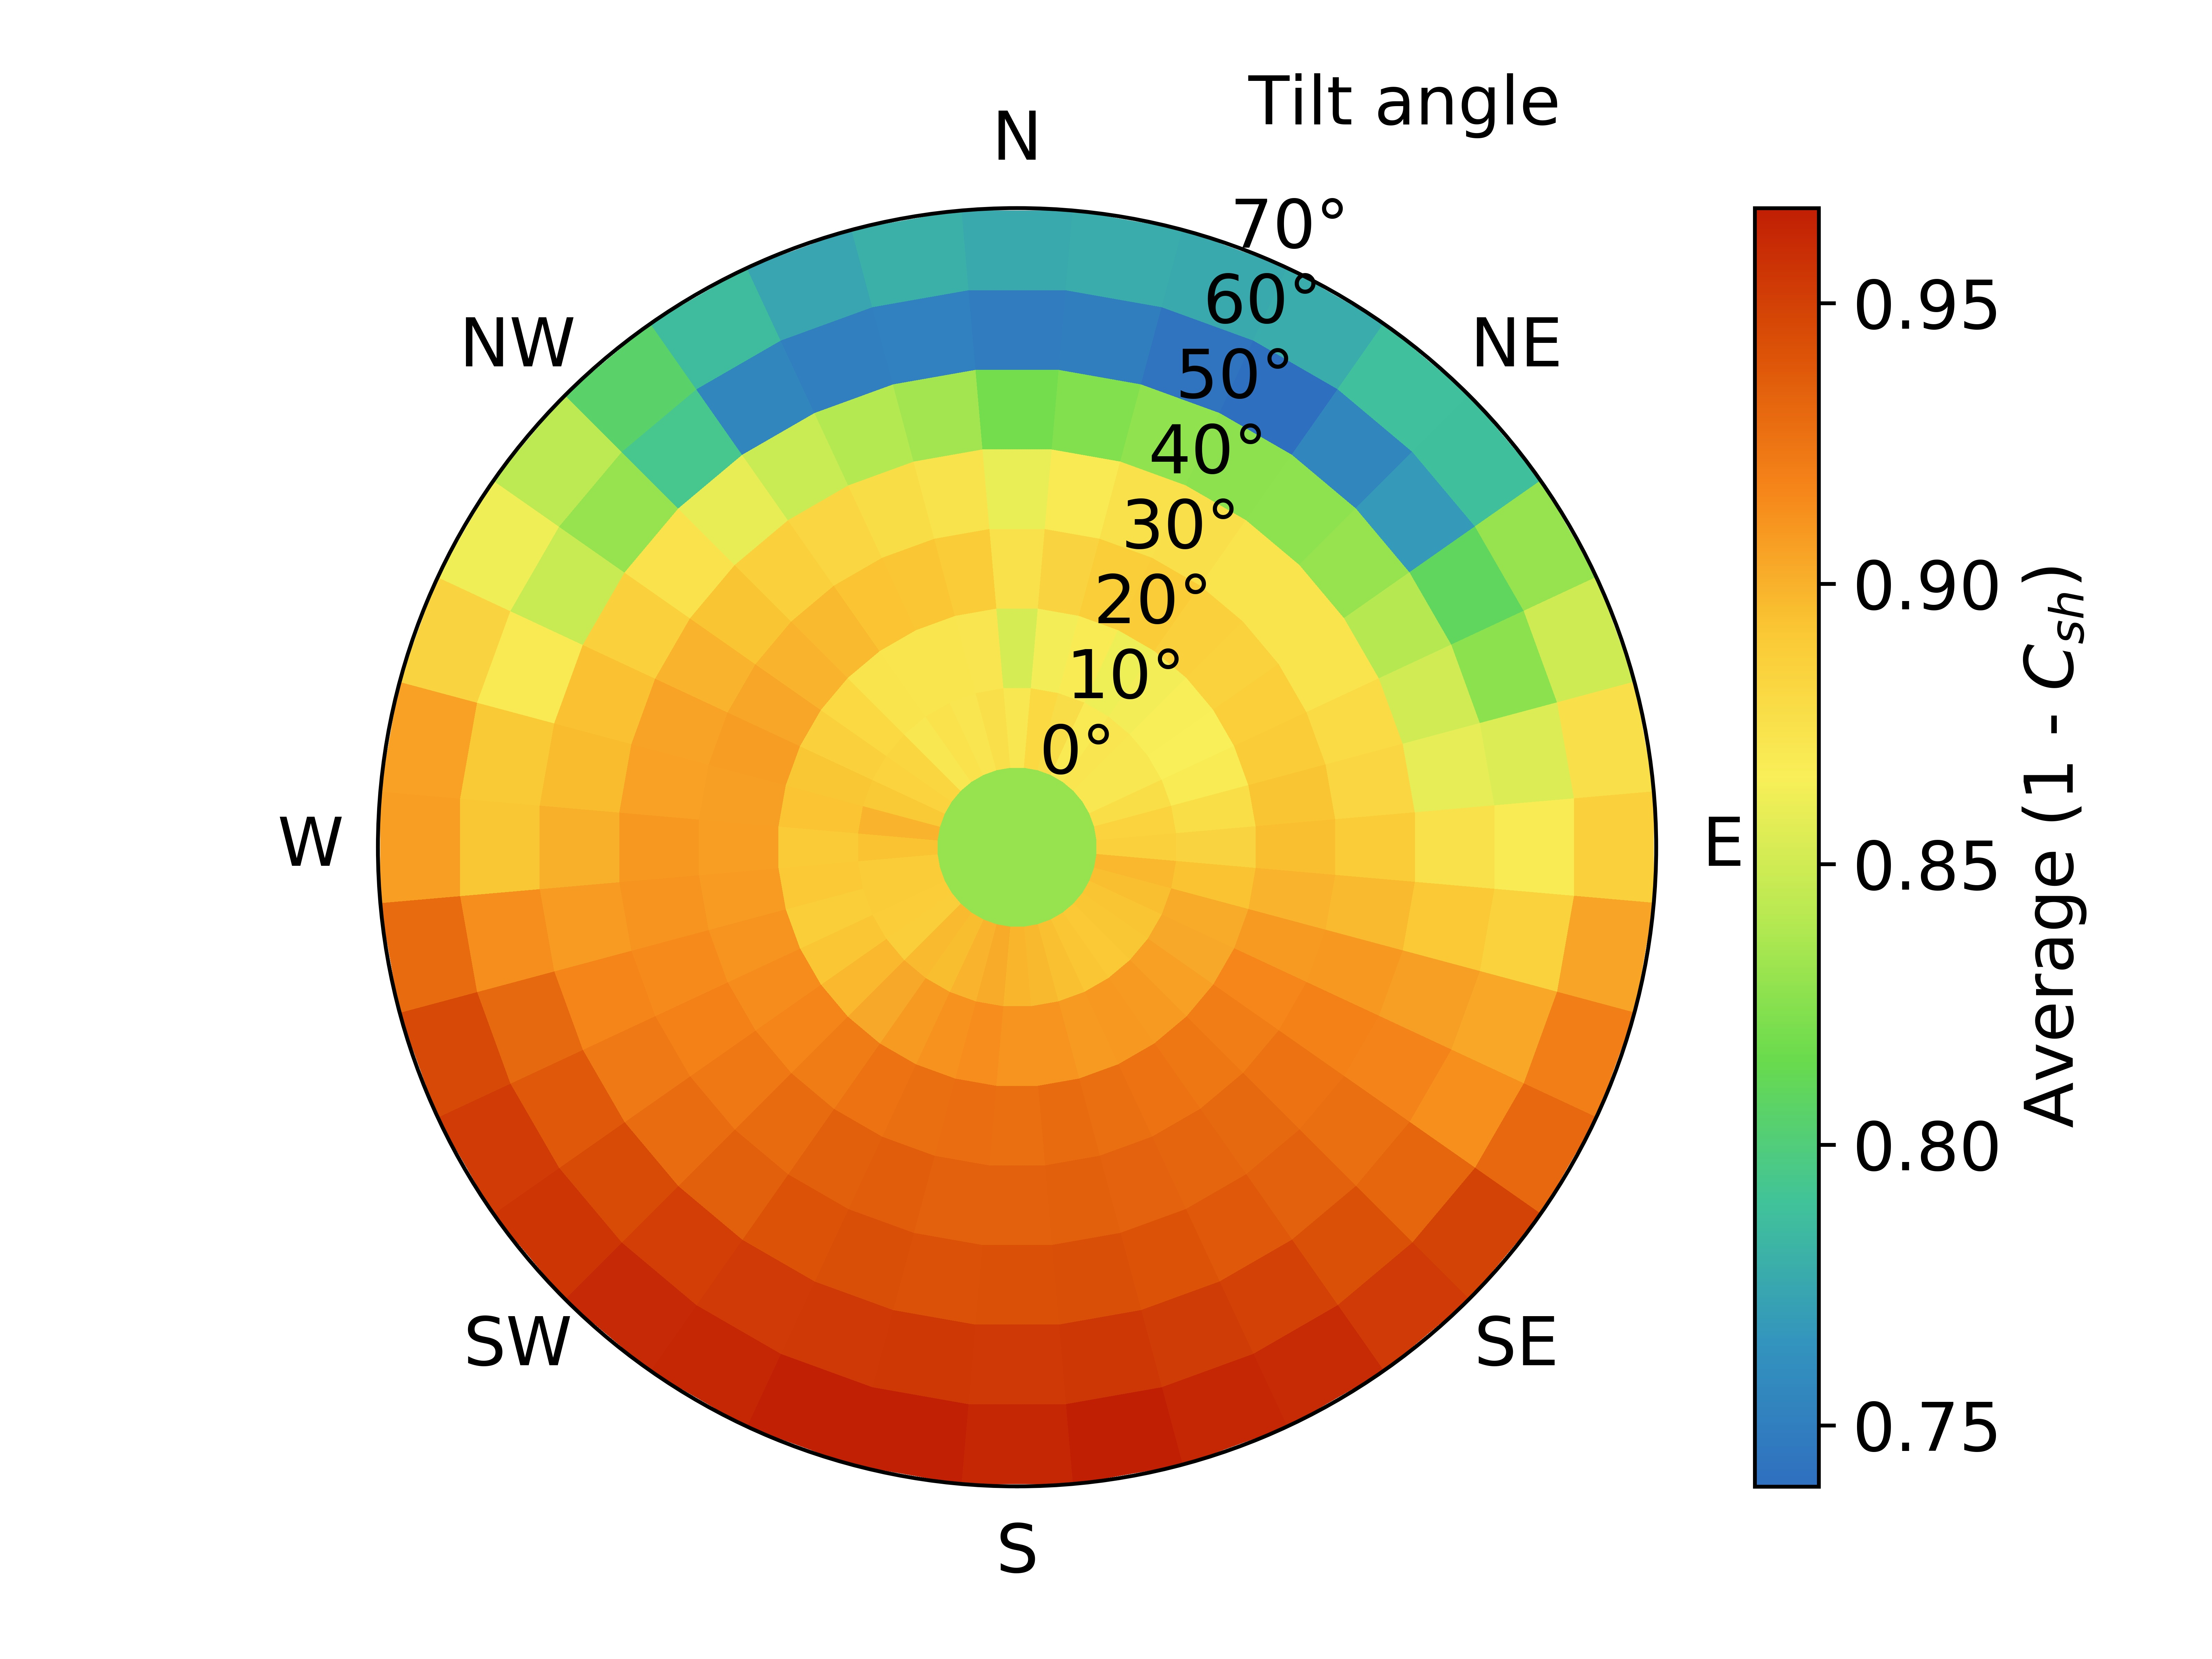
\includegraphics[width=0.9\linewidth]{Figs/Shade_slope_azimuth.jpg}
  \subcaption{}
\end{subfigure}
\begin{subfigure}{.49\textwidth}
  \centering
  % include first image
  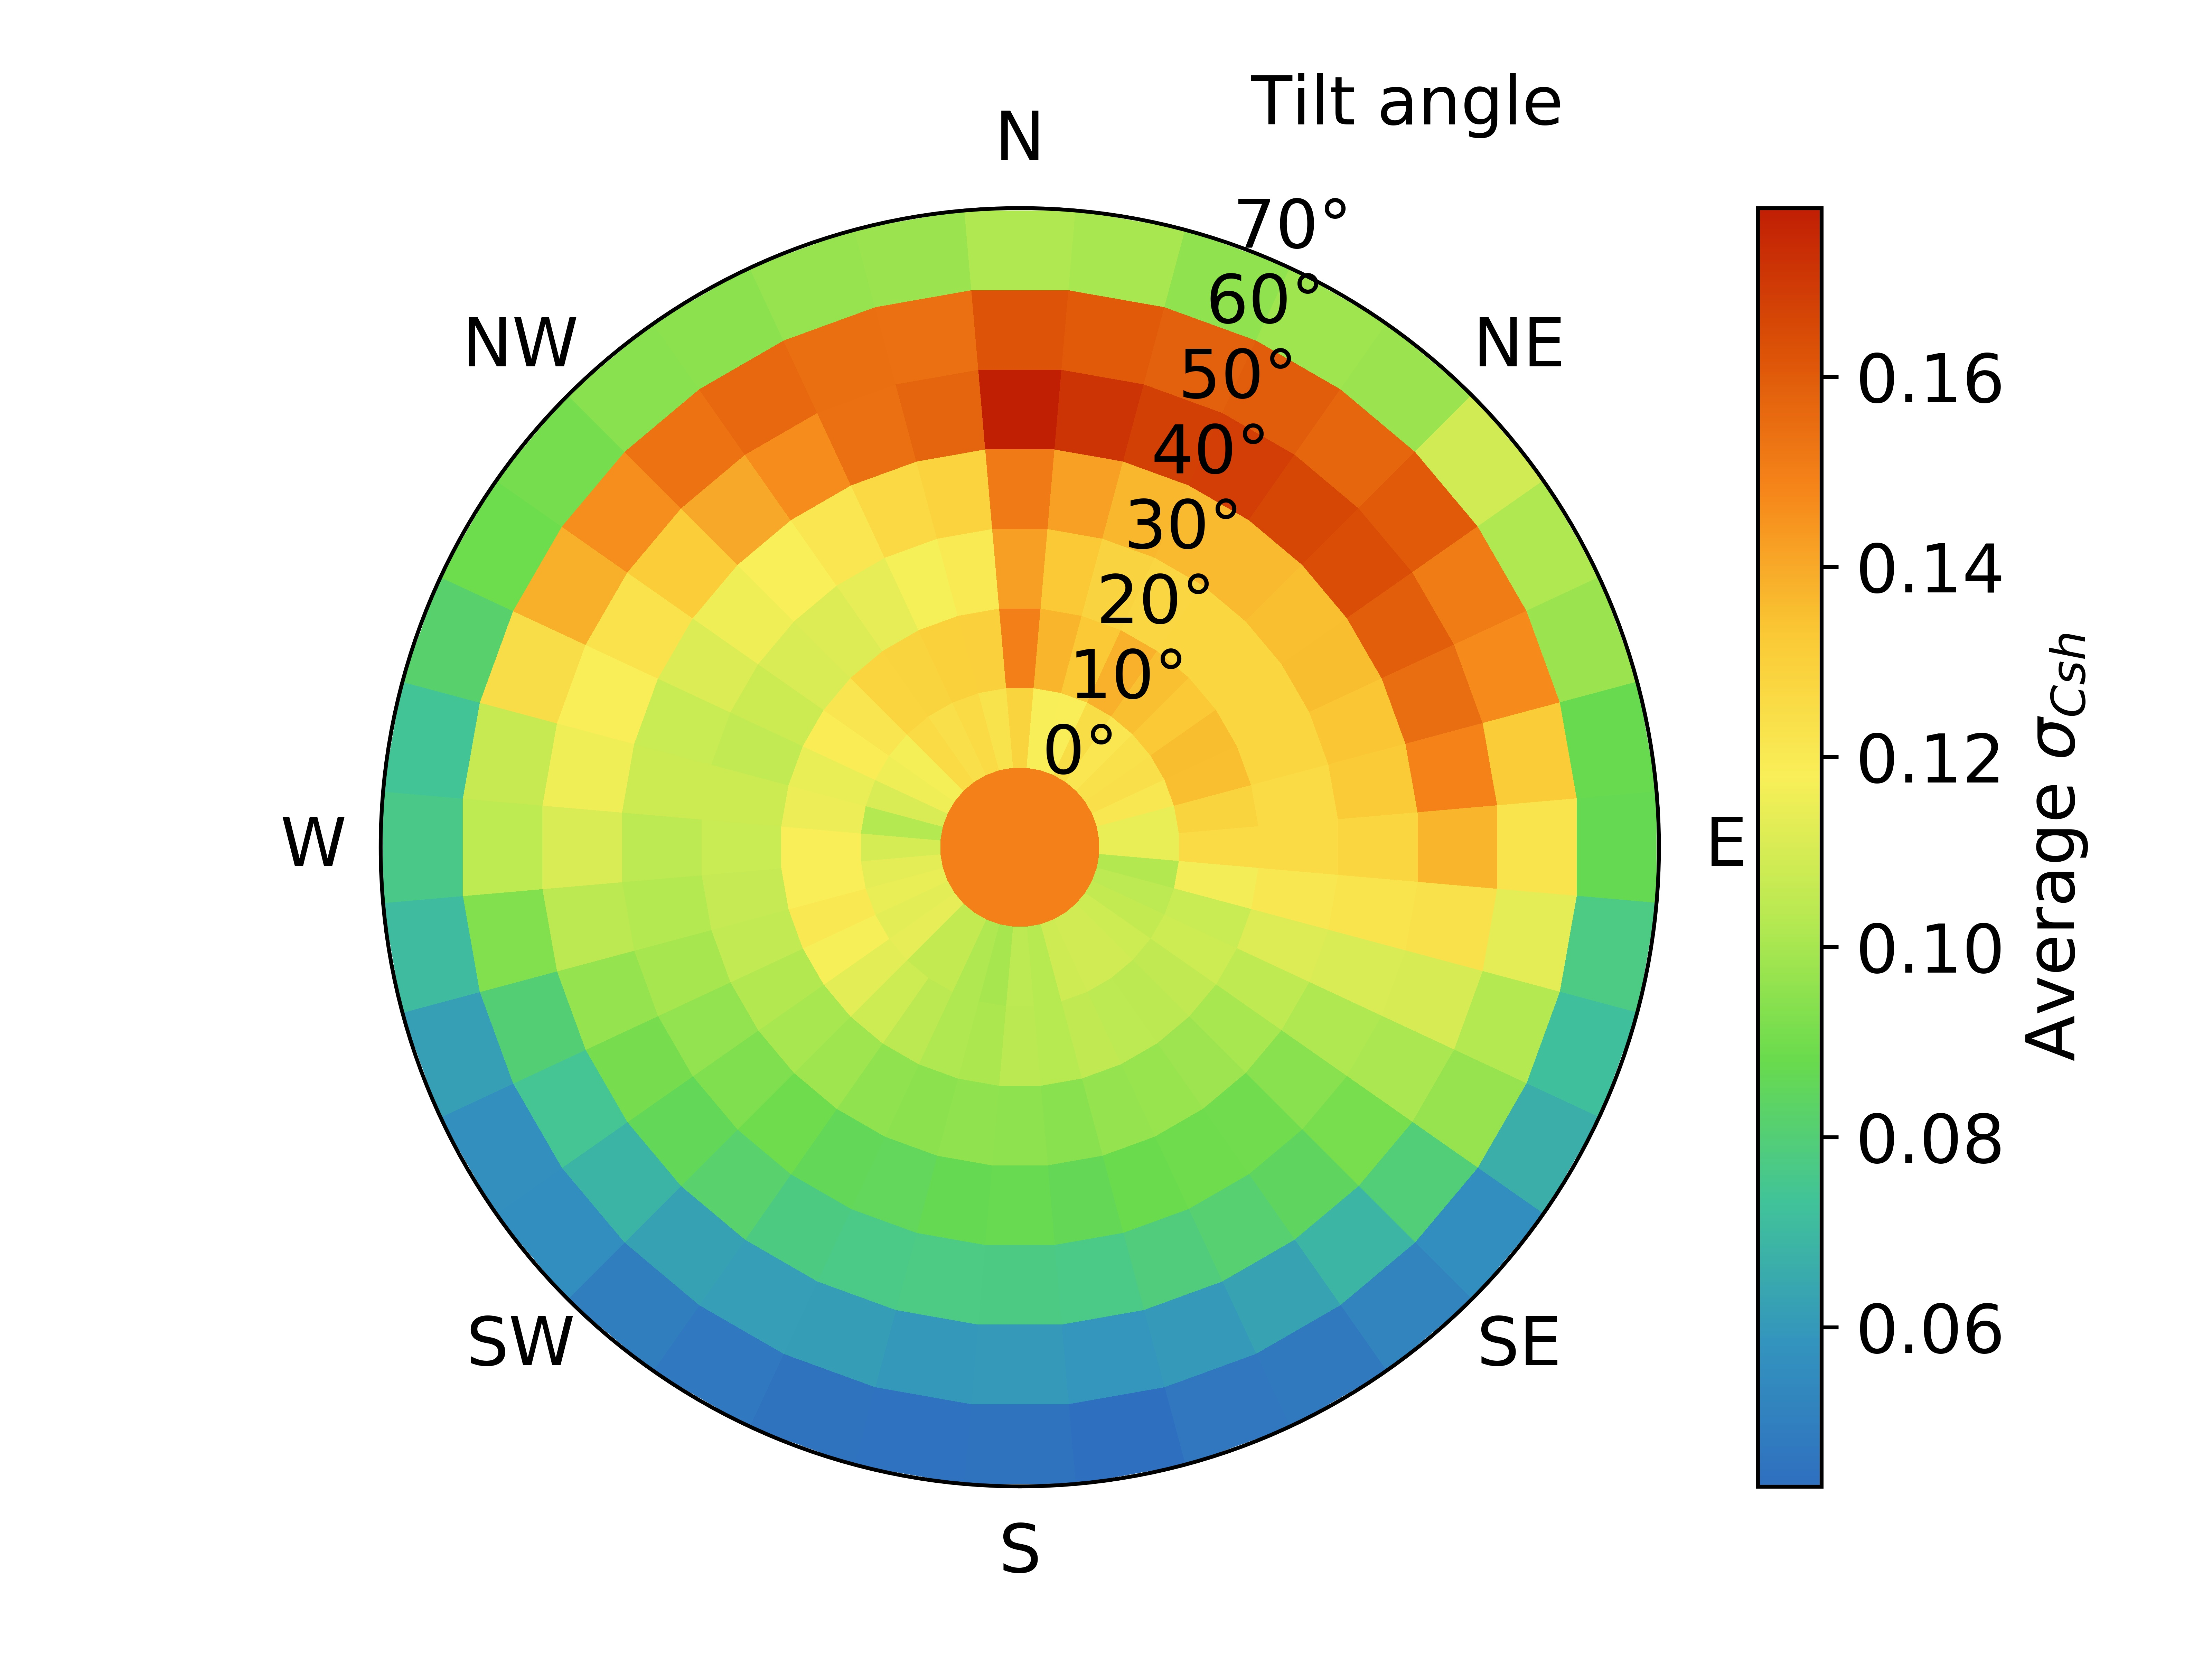
\includegraphics[width=0.9\linewidth]{Figs/Shade_slope_azimuth_unc.jpg}  
  \subcaption{}
\end{subfigure}
\caption{a) Proportion of roof area suitable for PV installation based on shading effects (1 - $C_{sh}$), b) its uncertainty $\sigma_{\mathit{Csh}}$ per roof aspect and tilt.}
\label{fig:Csh}
\end{figure}

The predicted values for $(1-C_{sh})$, grouped by roof aspect and tilt angles, are shown in Fig.~\ref{fig:Csh}a, with the related $\sigma_{\mathit{Csh}}$ shown in Fig.~\ref{fig:Csh}b. 
As expected, steep north-facing surfaces have the highest proportion of strongly shaded roof surface, i.e. the lowest values for $(1-C_{sh})$, while this value is highest for steep south-facing surfaces. 
Interestingly, flat surfaces (in the centre of  Fig.~\ref{fig:Csh}a) are significantly more shaded than roofs with a shallow tilt. This may be due to obstructing objects on flat surfaces or a stronger shading from surrounding buildings. 
The uncertainty is proportional to the shaded area coefficient and is hence highest for steep north-facing roofs. 

%%%%%%%%%%%%%%% Gt %%%%%%%%%%%%%%%%%%%%%%%

To compute $G_t$ from Eq.~(\ref{eq:irrad}) and its uncertainty $\sigma_{Gt}$ from Eq.~(\ref{eq:irrad_unc}), we combine the tilted radiation $G_{Bt,Dt,Rt}$ (Section \ref{app:irrad}) with the $S_{sh}$ (Section \ref{shade}) and the SVF (Section \ref{svf}).
%
Figure~\ref{fig:Sh}a shows the bias-corrected unshaded fraction $(1-S_{sh})$ for roofs of different tilts and aspects for four example hours in June. 
The patterns of $S_{sh}$ follow the trajectory of the sun, with shading on west-facing surfaces in the morning hours and shaded east-facing roofs in the evening.
Around solar noon (12h-14h), $S_{sh}$ is nearly zero for all roofs. This is expected as strongly shaded areas are already excluded (as part of $C_{sh}$). 
Figure~\ref{fig:Sh}b shows the related uncertainty $\sigma_{\mathit{Ssh}}$ (blue line), which is strongly correlated with the zenith angle of the sun (orange line). As the uncertainty primarily arises from the discrepancy between the DSM$_{2\text{m}}$ and the DSM$_{50\text{cm}}$, these results indicate that the discretization error of the DSM$_{2\text{m}}$ has a higher impact on $S_{sh}$ at low sun altitudes.
Consequently, the uncertainty is high in the morning and evening and low during midday in the summer months, when the solar radiation is highest. 
%
The average SVF on Swiss roofs is 0.69, with a $\sigma_{\mathit{SVF}}$ of 0.12 derived from the bias correction.

\begin{figure}[tb]
\centering
\begin{subfigure}{.98\textwidth}
    \centering
    
\includegraphics[width=0.9\linewidth]{Figs/Shade_hourly_slope_azimuth_row2.jpg} \subcaption{}
\end{subfigure}
\begin{subfigure}{.98\textwidth}
    \centering
    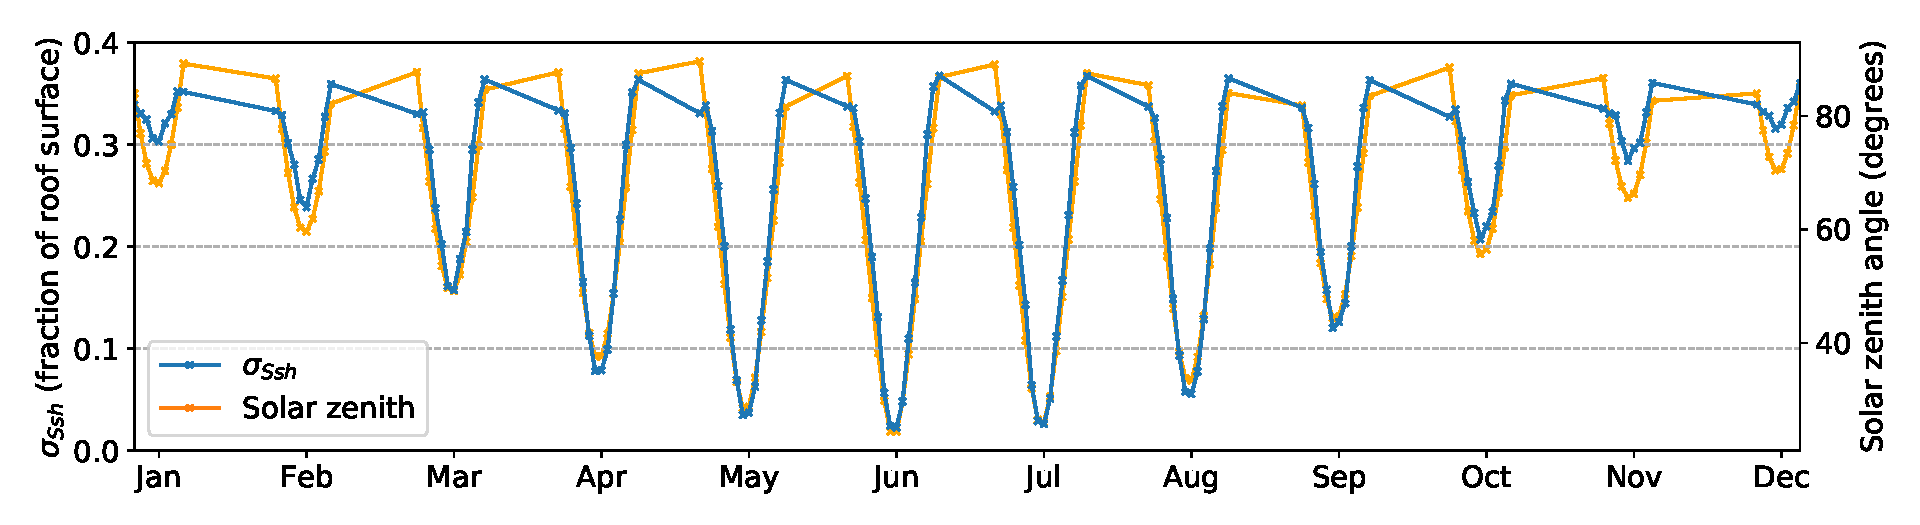
\includegraphics[width=0.9\linewidth]{Figs/Ssh_sigma_zenith2.pdf} 
    \subcaption{}
\end{subfigure}
\caption{a) Hourly unshaded fraction of suitable roof area ($1-S_{sh}$) for four example hours in June, averaged across roofs with equal aspect and tilt angles and b) its uncertainty $\sigma_{\mathit{Ssh}}$ as a function of time. The yellow line shows the bias between the two DSMs, for which we correct the values of $1-S_{sh}$.}
\label{fig:Sh}
\end{figure}

Figure~\ref{fig:Gt} shows the annual tilted irradiation on the building roofs ($G_t$) and its uncertainty ($\sigma_{Gt}$), again grouped by their tilt and aspect. The annual $G_t$ (a) is highest for south-facing roofs with a tilt angle of around $40^\circ$. This matches the latitude of Switzerland. As panels on flat roofs are oriented south and tilted at $30^\circ$, they receive near-maximum solar irradiation.
Fig.~\ref{fig:Gt}b shows $\sigma_{Gt}$ as percentage of $G_t$. It is lowest for steep north-facing roofs, which receive low direct radiation and are hence less impacted by $\sigma_{GB}$. 
The highest relative uncertainty is found on steep roofs in the east and the west. 
These roofs receive much direct radiation at low sun positions, for which $\sigma_{\mathit{Ssh}}$ is high.
%
Fig.~\ref{fig:Gt}c shows the hourly profiles for surfaces oriented north, east, west and south, averaged across all roofs of similar aspect. In summer, the peak of east-facing roofs in the morning is higher than that of the west-facing roofs in the afternoon. In winter, the opposite is the case. 
These results suggest that during summer the sky is clearer in the morning, while the weather is generally better in the afternoon in winter. 

\begin{figure}[tb]
\centering
\begin{subfigure}{.49\textwidth}
  \centering
  % include second image
  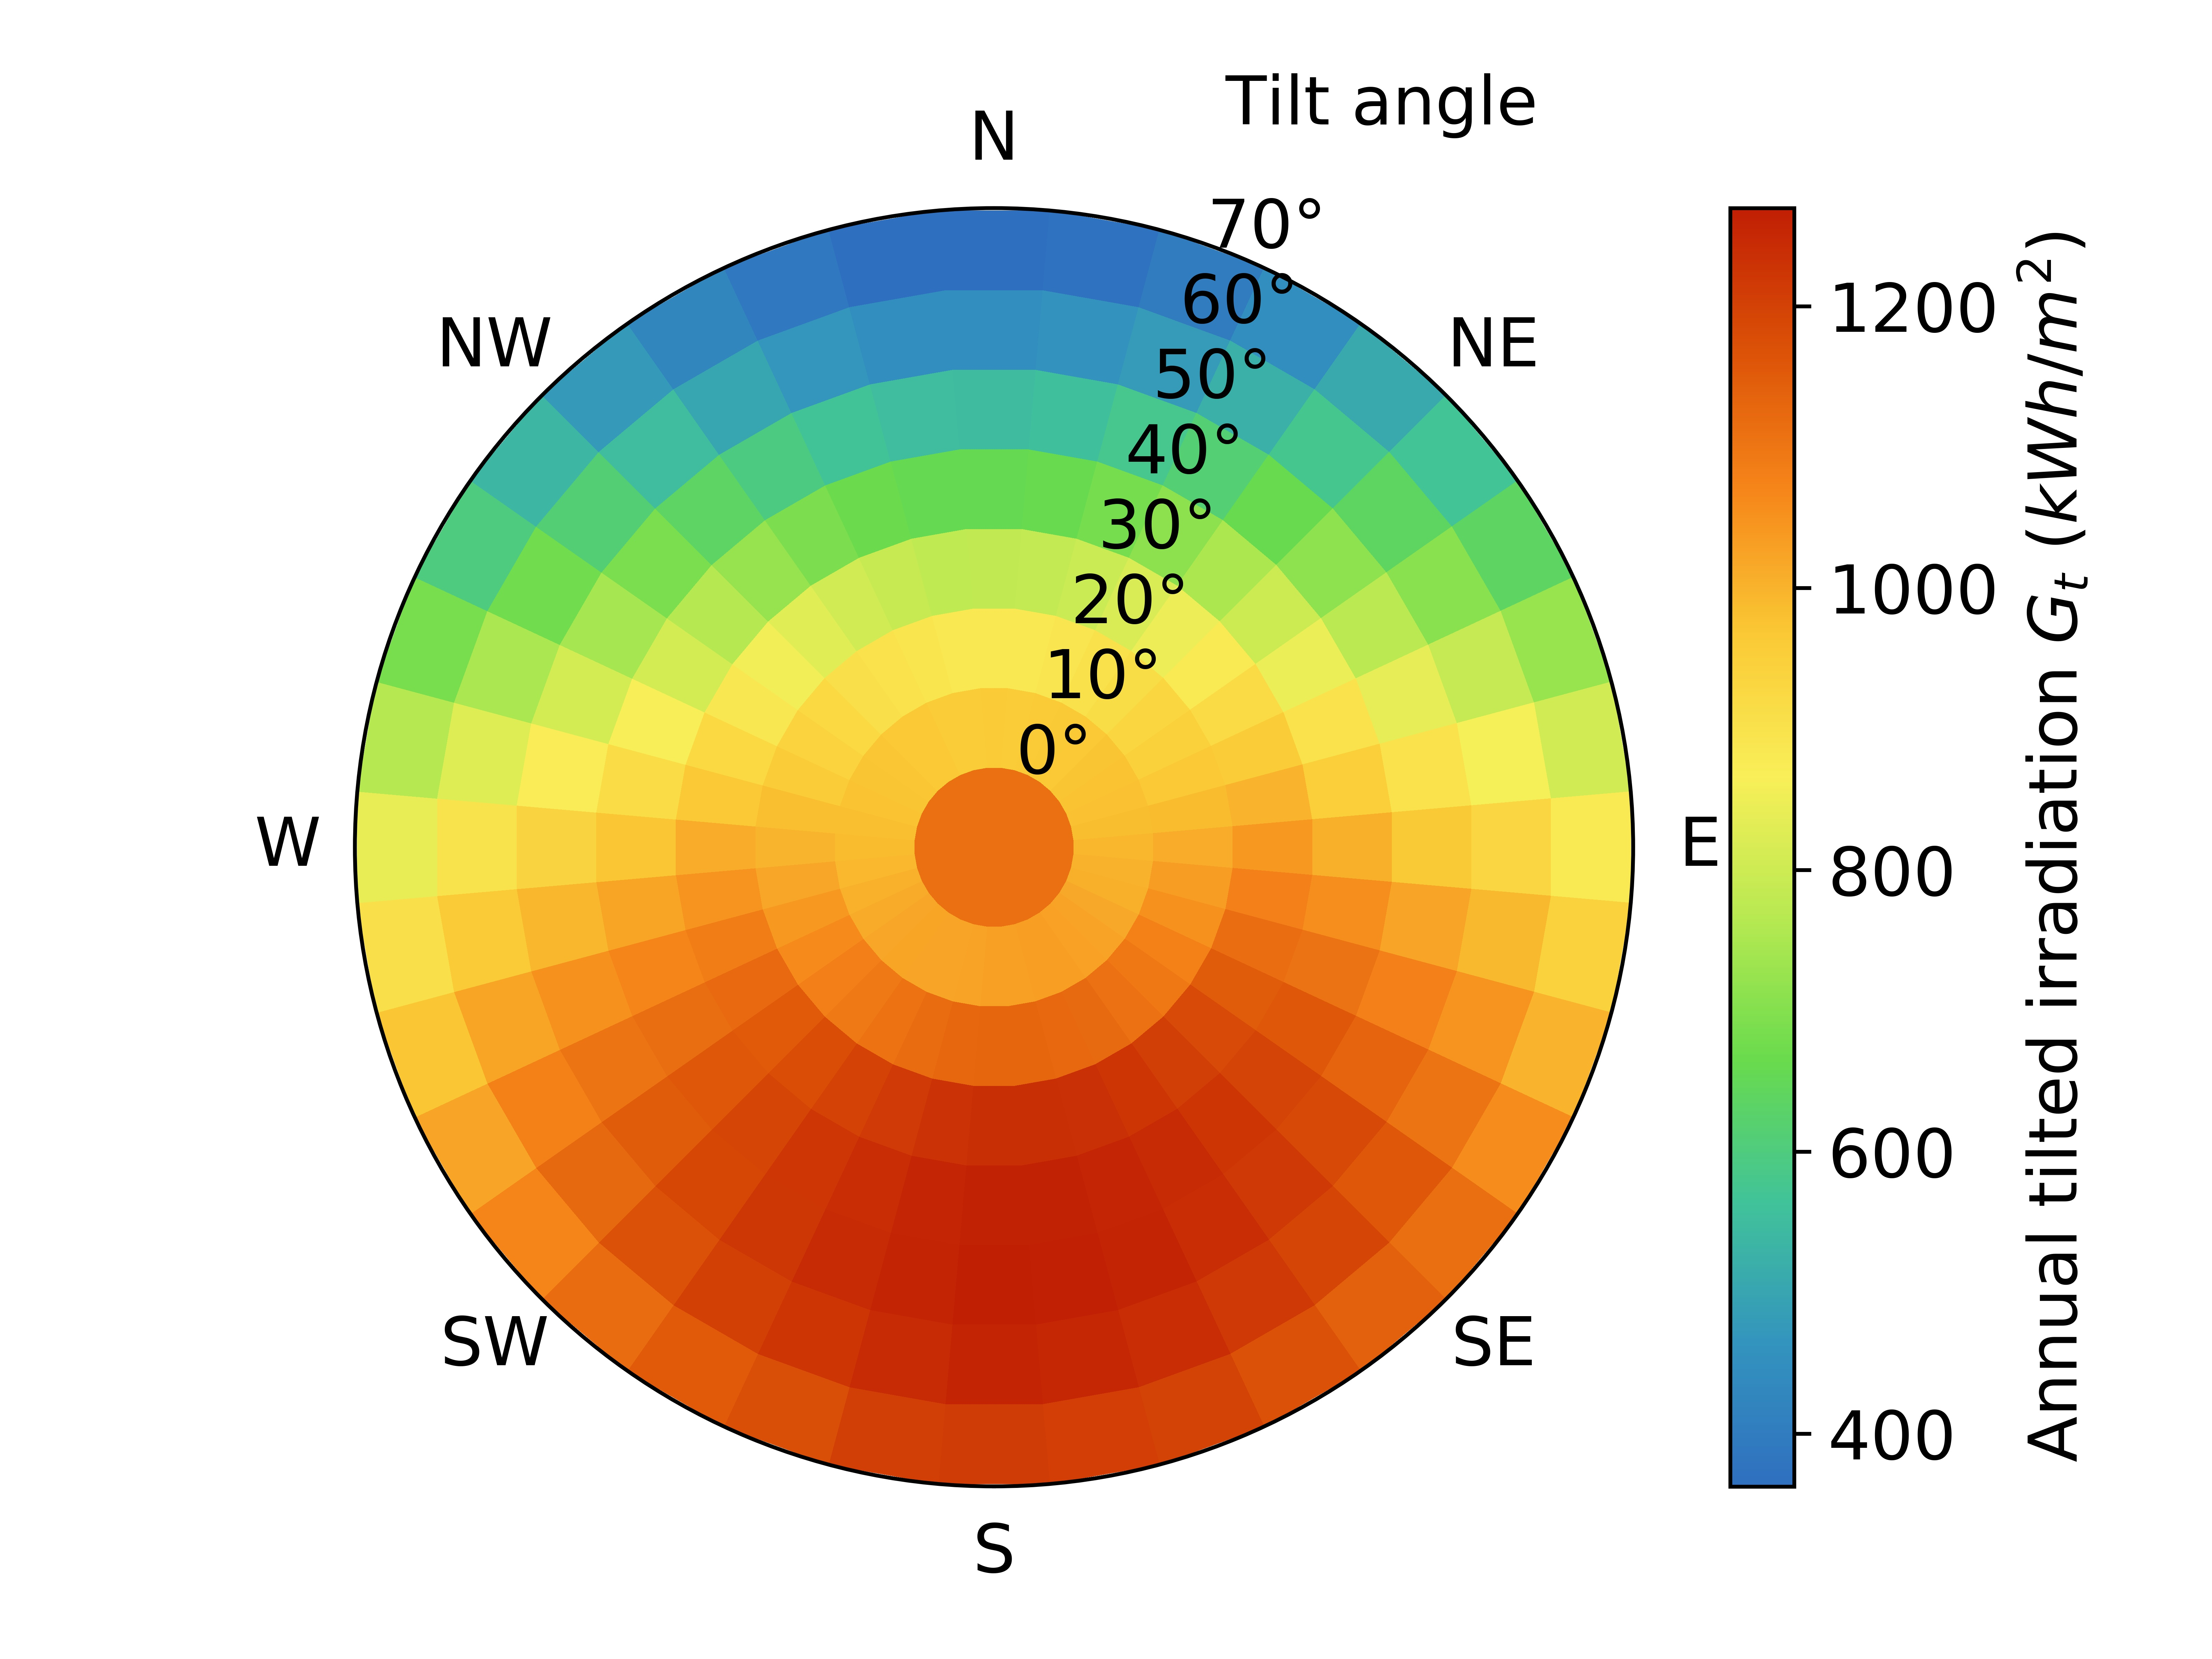
\includegraphics[width=0.9\linewidth]{Figs/annual_Gt.jpg}  
  \subcaption{}
\end{subfigure}
\begin{subfigure}{.49\textwidth}
  \centering
  % include first image
  \includegraphics[width=0.9\linewidth]{Figs/relative_unc_Gt.jpg}  
  \subcaption{}
\end{subfigure}
\begin{subfigure}{.9\textwidth}
  \centering
  % include first image
  \includegraphics[width=\linewidth]{Figs/Irrad_hourly_aspects.pdf} 
  \subcaption{}
\end{subfigure}
\caption{a) Annual tilted irradiation ($G_t$, in kWh/m$^2$) and b) relative annual uncertainty ($\sigma_{Gt} / G_t$) per roof aspect and tilt angle, c) MMH profiles of $G_t$ for north, east, west and south-facing roofs.}
\label{fig:Gt}
\end{figure}

%%%%%%%%%%%%%%%%%%%%%%%%%%%%%%%%%%%%%%%%%%%%%%%%%%%%%%%

\subsection{Technical potential estimation}
\label{solar_tech}

\begin{figure}[tb]
\centering
\begin{subfigure}{.48\textwidth}
  \centering
  % include first image
  \includegraphics[width=\linewidth]{Figs/PV_per_roof_area_tilt_norm.jpg} 
  \subcaption{}
  \label{figa:pv_roof}
\end{subfigure}
\begin{subfigure}{.48\textwidth}
  \centering
  % include second image
  \includegraphics[width=\linewidth]{Figs/PV_slope_azimuth_suitable_norm.jpg}
  \subcaption{}
  \label{figb:pv_roof}
\end{subfigure}
\caption{Annual technical RPV potential for all roof surfaces ($E_{PV}$, in kWh/m$^2$), a) grouped by roof tilt and area, b) grouped by roof tilt and aspect.}
\label{fig:pv_roof}
\end{figure}

To obtain the technical PV potential ($E_{PV}$) and its uncertainty ($\sigma_{PV}$), Eqs.~(\ref{eq:pv}) and (\ref{eq:pv_unc}) are applied to $G_t$, $A_{PV}$, the module efficiency ($\eta_{PV}$) and the performance factor ($\mathit{PF}$), which are obtained as described in Section~\ref{app:efficiency}.
%
Figure~\ref{fig:pv_roof} shows the annual $E_{PV}$ for Switzerland, grouped by its three main characteristics: tilt, aspect and roof area. For comparability, the values are normalized by the total roof area ($A_t$). 
Fig.~\ref{fig:pv_roof}a shows the potential with respect to roof tilt (x-axis) and roof area (y-axis), indicating the highest potential for large roofs ($> 500$ m$^2$) with shallow tilt. 
The similarity to the pattern of $C_{\mathit{pv}}$ in Fig.~\ref{fig:C_pv}a demonstrates the strong dependency of $E_{PV}$ on $C_{\mathit{pv}}$.
As a consequence, the peak potential in Fig.~\ref{fig:pv_roof}b is no longer at 40$^\circ$ south, as it is the case for $G_t$ (see Fig.~\ref{fig:Gt}), but it appears instead at around 10$^\circ$, which is the tilt angle of many large roofs. 
% This is due to the high potential of large roofs ($>500m$^2$) at this tilt angle. 
Flat roofs, on the other hand, show a relatively smaller potential, due the strategy for installing PV panels on flat roofs explained in Section \ref{flat}.

To obtain a realistic large-scale potential estimate, we exclude roofs with a small available area of $A_{PV}<8$ m$^2$~\cite{assouline_large-scale_2018}, which represents a minimal economic feasibility \cite{assouline_quantifying_2017, assouline_large-scale_2018, portmann_sonnendach.ch:_2016, romero_rodriguez_assessment_2017}. 
We further exclude all north-facing roofs with an aspect angle $|\gamma| > 90^\circ$ from south~\cite{assouline_large-scale_2018, assouline_quantifying_2017}, which aims at removing those roofs with a low PV potential. Other studies use a minimum annual $G_t$ of 1000 kWh/m$^2$ \cite{buffat_scalable_2018, portmann_sonnendach.ch:_2016, romero_rodriguez_assessment_2017}. This threshold however is found to be sensitive to small changes in the estimated potential, so we use the aspect angle as selection criterion instead.

\begin{figure}[b]
\centering
\begin{subfigure}{.63\textwidth}
  \centering
  % include second image
  \includegraphics[width=0.9\linewidth]{Figs/PV_per_pixel_small.jpg}
  \subcaption{}
\end{subfigure}
\begin{subfigure}{.34\textwidth}
  \centering
  % include second image
  \includegraphics[width=0.9\linewidth]{Figs/PV_MWh_roofs.jpg}
  \subcaption{}
\end{subfigure}
\begin{subfigure}{.95\textwidth}
  \centering
  % include first image
  \includegraphics[width=.9\linewidth]{Figs/PV_hourly_w_unc_demand.pdf} 
  \subcaption{}
\end{subfigure}
\caption{a) Spatial distribution of annual $E_{PV}$, aggregated to pixels of $500 \times 500$ m$^2$ for visualization purposes, 
b) annual $E_{PV}$ for the suitable roofs of a randomly selected $500 \times 500$ m$^2$ pixel in the city of Geneva,
c) monthly-mean-hourly profiles of $E_{PV}$, summed for all suitable roofs, the $\sigma_{PV}$ and the Swiss electricity demand of 2018.}
\label{fig:results}
\end{figure}

Applying these criteria to all 9.6 million roof surfaces in Switzerland, 2.7 million roofs on 2.3 million buildings remain suitable to install PV panels. 
In total, the $A_{PV}$ is $267 \pm 71$ km$^2$ and the resulting maximum technical PV potential is $25 \pm 9$ TWh. Figure~\ref{fig:results}a shows the spatial distribution of the annual $E_{PV}$ aggregated to pixels of $500 \times 500$ m$^2$ for visualisation purposes. The potential is centered in the Swiss plateau, where most densely populated cities are located.
%
The annual $E_{PV}$ per rooftop of one such pixel is shown in Figure~\ref{fig:results}b, which demonstrates that large flat roofs have by far the highest potential to install PV panels.
%
Figure~\ref{fig:results}c shows the temporal variation of the PV potential and its total uncertainty, in comparison with the Swiss electricity demand of 2018 \cite{swissgrid_production_2019}. In absolute terms, the uncertainty is highest during the summer, due to a high variability of the horizontal radiation. The RPV potential exceeds the electricity demand even for the lower boundary of $E_{PV}$ ($E_{PV} - \sigma_{PV}$) from March until September, while a deficit is expected from November to January and during night hours. 

\subsection{Sensitivity analysis}

We conduct a sensitivity analysis to quantify the impact of the individual parameters computed in this study on the technical PV potential. The analysis is performed in two stages: firstly, each parameter is independently varied in a fixed range of $\pm 50\%$. 
In a second step, all parameters with a quantifiable uncertainty are varied by $\pm \sigma$. 
Due to the high correlation of the horizontal radiation components, $G_h$ and $G_B$ are varied simultaneously. A representative sample of 10,000 rooftops has been used for this analysis.

Figure \ref{fig:sens_vars}a shows the change in technical PV potential for varying each parameter by $\pm 50\%$. The horizontal radiation components ($G_h$), and the fractions of available roof area ($C_{sh}, C_{\mathit{pv}}$) are the most sensitive parameters and thus exhibit the steepest slope. 
This is expected, as these variables are directly correlated with the factors in the computation of $E_{PV}$ (see Eq.~(\ref{eq:pv})). 
As the panel efficiency reduces slightly for high $G_h$, its sensitivity curve lies just below $C_{sh}, C_{\mathit{pv}}$.
Changes in $S_{sh}$ and $\mathit{SVF}$ have a smaller impact on the RPV potential, as they are multiplied with $G_{Bt}$ and $G_{Dt}$, respectively. 
The curves flatten out for large positive changes, as both factors are saturating at a value of 1. 
The albedo ($\rho$) has a very low sensitivity, as there are few steep roofs that are impacted by a change in $\rho$.
The ambient temperature ($T_{amb}$) is the only curve with a negative slope, as high temperatures decrease $\eta_{PV}$. Its sensitivity is rather low, as $T_{amb}$ only indirectly impacts the PV potential as part of the physical model of $\eta_{PV}$. 

\begin{figure}[b]
\centering
\begin{subfigure}{.49\textwidth}
  \centering
  % include second image
  \includegraphics[width=\linewidth]{Figs/sensitivity_vars_Tamb.pdf}
  \subcaption{}
  \label{figa:sens_vars}
\end{subfigure}
\begin{subfigure}{.49\textwidth}
  \centering
  % include first image
  \includegraphics[width=\linewidth]{Figs/sensitivity_unc.pdf}  
  \subcaption{}
  \label{figb:sens_vars}
\end{subfigure}
\caption{Change in RPV potential for the variation of a) each variable by $\pm 50\%$ and b) each uncertain variable by $\pm \sigma$. Considered variables are the horizontal radiation ($G_h$), partly shading factor ($S_{sh}$), sky view factor ($\mathit{SVF}$), surface albedo ($\rho$), shaded and panelled area ratios ($C_{sh}, C_{\mathit{pv}}$) and ambient temperature ($T_{amb}$).}
\label{fig:sens_vars}
\end{figure}

Figure \ref{fig:sens_vars}b shows the impact of varying each variable within their uncertainty ($\pm \sigma$). 
The upper and lower dashed lines represent the propagated $\sigma_{PV}$. 
The results suggests that in a year with low $G_h$, the electricity generation may be up to 18\% lower than estimated, and similarly for the higher case. 
The $S_{sh}$ and $\mathit{SVF}$ show the lowest sensitivity, which agrees with Fig.~\ref{fig:sens_vars}a.
Comparing $C_{\mathit{pv}}$ and $C_{sh}$ shows that $\sigma_{\mathit{Cpv}}$, driven by the high uncertainty of medium-sized roofs, is overall larger than $\sigma_{\mathit{Csh}}$, with a potential impact of $\pm 11 \%$. 
%
The bars in Fig.~\ref{fig:sens_vars}b indicate the potential change when all roofs are considered, while the lines show the potential change for the suitable roofs only (see Section~\ref{solar_tech}). 
For $G_t$, the suitable south-facing roofs have a higher uncertainty than all roofs, as expected from Fig~\ref{fig:Gt}b. 
The opposite is the case for $A_{PV}$, as the suitable roofs have a higher proportion of flat roofs with a low $\sigma_{\mathit{Cpv}}$.



%%%%%%%%%%%%%%%%%%%%%%%%%%%%%%%%%%%%%%%%%%%%%%%%%%%%%%%
%%%%%%%%%%%%%%%%%%%%%%%%%%%%%%%%%%%%%%%%%%%%%%%%%%%%%%%

\section{Comparison to existing studies}
\label{solar_comparison}

\begin{comment}
Installing photovoltaics (PV) on building rooftops is a promising approach to reduce greenhouse gas emissions, especially in dense urban areas. Understanding the large-scale potential for rooftop PV is important for several reasons, including electricity network design, urban and regional energy planning, as well as incentive policies for PV installations. Several studies in recent years focus on assessing a large-scale technical rooftop PV potential. Early methods relying on “rules of thumb” \cite{iea_potential_2002} have been continuously improved by incorporating environmental and building data as well as using powerful computational engines and advanced analytic methods such as Machine Learning (ML). This progress in data processing, enabled by the availability of larger and more accurate datasets, has led to widely varying results of PV potential studies, even for the same geographic area. This makes the comparison across studies intrinsically challenging. \citet{assouline_estimation_2017} provide an overview of the existing methods to estimate a large-scale technical rooftop PV potential, however this methodological review does not discuss the results obtained by individual studies. Some of these compare their results with those of other studies, but the discrepancies are explained in a qualitative rather than quantitative way \cite{assouline_quantifying_2017,assouline_large-scale_2018}. 
\end{comment}

To set the results from Section~\ref{solar_results} into context, we compare them to five existing national-scale studies of RPV potential for Switzerland, which have been carried out from 2002-2018 \cite{iea_potential_2002,assouline_quantifying_2017,assouline_large-scale_2018,klauser_solarpotentialanalyse_2016,buffat_scalable_2018}.
% In this Section, we propose a framework to compare large-scale rooftop PV assessment studies in a quantitative way. 
This helps to understand how different methods and hypotheses impact the potential estimates. 
% We focus the comparison on Switzerland, where six have been carried out at national scale from 2002 to 2020 
The six compared studies, including this work, are:
% The results are interpreted with respect to the following aspects: (i) target audience, (ii) spatio-temporal resolution, (iii) datasets, and (iv) methods. 
% We finally provide a perspective on future developments which may further improve the PV potential studies. 
% The comparison is based on the following studies: 

\begin{enumerate}
\item The first study (\textit{\textbf{S1}}) was conducted for several European countries including Switzerland by the International Energy Agency (IEA) in 2002 \cite{iea_potential_2002}. The method is based on rules of thumb, established at European scale, and does not reflect the local Swiss building stock. The technical potential is a yearly value for the entire country. This represents the lowest temporal and spatial resolution among the compared studies, indicating an order of magnitude of the total technical rooftop PV potential at national scale. 
\item The second study (\textit{\textbf{S2}}) for Switzerland was conducted by \citet{assouline_quantifying_2017} at commune scale. In this study, a Machine Learning algorithm, Support Vector Machines (SVM), combined with Geographic Information Systems (GIS), is used in order to estimate the technical PV potential on building rooftops. ML is used as an effective method of extrapolation to solve problems of data availability in parts of the study area. The study is performed at monthly-mean-daily temporal resolution for all Swiss communes. 
\item The third study (\textit{\textbf{S3}}) is again conducted by \citet{assouline_large-scale_2018} at $200 \times 200$ m$^2$ spatial resolution. In this study, another ML algorithm, Random Forests (RF), is used in combination with GIS to estimate the potential. The method from S3 is enhanced in S4 using (i) larger and more accurate datasets, (ii) a more efficient  ML algorithm that includes the estimation of model uncertainties, and (iii) a higher spatial resolution of $200 \times 200$ m$^2$. Both studies aim at a large-scale estimation of PV potential on building roofs to inform regional and national decision making.
\item The fourth study (\textbf{\textit{S4}}) was conducted as a national project, namely Sonnendach.ch, by the Swiss Federal Offices of Energy (SFOE), Topography (Swisstopo), and Meteorology and Climatology (MeteoSwiss) \cite{klauser_solarpotentialanalyse_2016,portmann_sonnendach.ch:_2016}. Monthly solar PV potential is estimated for each rooftop in Switzerland using a GIS-based approach \cite{klauser_solarpotentialanalyse_2016} complemented by rules of thumb \cite{portmann_sonnendach.ch:_2016}. In contrast to the above studies (S1-S3), the primary target group of this study is individual property owners and energy service providers interested in installing PV on specific building roofs. Thus, the primary output of this study is a classification of rooftop suitability for solar PV installation.
\item The fifth study (\textbf{\textit{S5}}), conducted by \citet{buffat_scalable_2018}, estimates PV potential from solar radiation profiles in half-hour temporal resolution for pixels of $0.5 \times 0.5$ m$^2$. In this study, GIS is used to estimate the solar radiation on tilted surfaces. In addition, the study includes a detailed model of the panel and inverter efficiencies. The results presented in the study aim primarily at a comparison between different PV technologies and are validated against measurement data.
\item The sixth study (\textbf{\textit{S6}}) is the estimation of solar PV potential presented above and published in \cite{walch_big_2020}. As explained in Section~\ref{solar_method}, Geographic Information Systems and Machine Learning approaches are used to estimate the solar PV potential for each building roof surface at hourly temporal resolution.
ML is used to quantify not only the modelling uncertainty for the resulting PV potential estimation, but also the uncertainty in the data. The hourly temporal resolution of the results is important for the spatio-temporal modelling of future electricity systems.   

\end{enumerate}
\subsection{Methodological comparison}

To compute the technical rooftop PV potential, the hierarchical approach presented in Chapter~\ref{method_solar_hierarchy} is used in all studies, which differentiates between physical potential, geographic potential and technical potential.
%
% The physical potential is defined as the global horizontal solar radiation ($G_h$), consisting of a direct horizontal ($G_B$) and a diffuse horizontal ($G_B$) component. 
To estimate the physical potential, a constant global horizontal radiation ($G_h$) of 1,167 kWh/m$^2$ (from Meteonorm) is used in S1 for the entire country. In all other studies (S2-S6), the global, direct and diffuse horizontal radiation components ($G_h$, $G_B$,$G_D$) are obtained from satellite-derived solar radiation data based on the Heliosat algorithm \cite{rigollier_method_2004}. S2 and S3 use this data for 100 locations, S5 uses a gridded dataset at $3.8 \times 5.6$ km$^2$ spatial resolution (SARAH) and S4 and S6 use data on a $1.6 \times 2.3$ km$^2$ grid provided by MeteoSwiss, which contains improvements for radiation modelling at high altitude \cite{stockli_heliomont_2017}. S4 and S5 directly use the input data as physical potential. S2, S3 and S6 use Machine Learning to derive $G_h$, $G_B$ and $G_B$ on a $200 \times 200$ m$^2$ grid to better represent the local terrain. In S2 and S3, measurements of temperature, precipitation, sunshine duration and cloud cover are used to support the estimation, while S6 use spatial features (coordinates and altitude) only. 

The geographic potential is driven by two factors: (i) tilted radiation ($G_t$, in kWh/m$^2$) and (ii) available area for PV panel installation ($A_{PV}$, in m$^2$). For this comparison of large-scale RPV potential estimations, we propose to define $G_t$ and $A_{PV}$ in a general form as:

\begin{equation}
\label{eq:Gt_compare}
    G_t = (1 - Sh_A) (Sh_{Bt} * G_{Bt} + \mathit{SVF} * G_{Dt} + G_{Rt})
\end{equation}

\begin{equation}
\label{eq:APV_compare}
    A_{PV} = A_{\mathit{floor}} * C_R \quad \forall A_{PV} > A_{min} 
\end{equation}

where $G_{Bt}$, $G_{Dt}$ and $G_{Rt}$ are the tilted radiation components (Section \ref{phys_models}), $Sh_A$ and $Sh_{Bt}$ are parameters of shading losses, explained below, \textit{SVF} denotes the sky view factor, $A_{\mathit{floor}}$ is the ground floor area, $C_R$ denotes the ratio of available area for PV panel installation over ground floor area and $A_{min}$ describes the minimum roof area considered for PV installation. 
These equations differ slightly from those presented in Section~\ref{solar_method} (Eq.~\ref{eq:irrad} and \ref{eq:area}) in order to be generalisable across all compared studies. 

Despite following the same physical principles, differences in spatio-temporal resolution and available datasets lead to significantly varying methods for calculating the parameters for geographic potential, as summarized in Table \ref{tab:compare_methods}. It should be noted that probabilistic functions are used in S2 and S3 to compute the geographic potential as detailed roof shapes are unknown. One exception to Eqs.~\ref{eq:Gt_compare} and \ref{eq:APV_compare} is S1, where the geographic potential is computed in a simplified way. In S1, $G_t$ is obtained by multiplying $G_h$ with an average solar yield ($\sim 93.3\%$ for Switzerland, derived from \cite{iea_potential_2002}). $A_{PV}$ is computed by multiplying an estimated floor area (45 m$^2$ per person) with the population size and a constant ratio of “architecturally suitable area / ground floor area”, equal to 0.72. This accounts for construction elements (here $C_R$) as well as shading (here $Sh_A$) \cite{iea_potential_2002}.

\begin{table}[tb]
\centering
\footnotesize
\caption{Comparison of methods for computing the main parameters of rooftop PV potential.}
\label{tab:compare_methods}
\resizebox{\textwidth}{!}{%
\begin{tabular}{lcccccc}
\hline
\textit{\textbf{Parameter}} & \textbf{S1}           & \textbf{S2}                     & \textbf{S3}   & \textbf{S4}          & \textbf{S5}    & \textbf{S6}         \\ \hline
$G_{Bt}, G_{Dt}, G_{Rt}$               & $G_h$ * \textit{yield}            & Daily                           & Daily         & Hourly               & Hourly         & Hourly              \\
\textit{SVF}                & -                     & 0.9                             & 0.9           & Horizon              & 1              & 0.9                 \\
$Sh_{Bt}$                        & -                     & Hillshade                       & Hillshade     & Horizon              & Horizon        & Horizon             \\
$Sh_A$                         & \multirow{2}{*}{0.72} & Hillshade = 0                   & Hillshade = 0 & 0                    & 0              & $\overline{Sh}_{Bt}$ \textless   40\% \\
$C_R$                          &                       & SP                              & SP + VP       & 0.42 – 0.8           & 1              & SP + VP             \\
$A_{min}$                        & -                     & 28 m$^2$                            & 8 m$^2$           & 10 m$^2$                 & -              & 8 m$^2$                 \\
\textit{Suitable roofs}     & 55\% of roofs         & \multicolumn{2}{c}{roof aspect $\in [-90^\circ,   90^\circ]$}          & \multicolumn{2}{c}{$G_t > 1000$ }       & as S2/S3            \\
$\eta$                      & \multirow{2}{*}{10\%} & 17\%                            & 17\%          & 17\%                 & Panel model    & Panel model         \\
\textit{PF}                 &                       & 80\%                            & 80\%          & 80\%                 & Inverter model & Inverter model      \\ \hline
\end{tabular}
}
\end{table}

In S2-S6, shading effects ($Sh_A$, $Sh_{Bt}$) are computed separately from $C_R$ using GIS and a DSM. All studies use Switzerland’s DSM in $2 \times 2$ m$^2$ resolution (see Chapter~\ref{data_DEM}). S4 and S5 interpolate this DSM to a $0.5 \times 0.5$ m$^2$ resolution. We distinguish between two types of shading, namely (i) the fraction of a roof area in full shade ($Sh_A$), and (ii) the average amount of shading on the remaining roof ($Sh_{Bt}$), reducing the direct tilted radiation. $Sh_A$ is only considered in S2, S3 and S6. S2 and S3 follow a Hillshade (HS) approach which estimates shading by computing relief maps for each pixel of a DSM. $Sh_A$ is obtained from pixels with a HS value of 0, while $Sh_{Bt}$ is obtained by averaging the remaining pixels over a building roof. 

ML is used by S2 and S3 to estimate shading effects at commune and pixel scale for Switzerland based on data from Geneva Canton. In contrast, S4-S6 use a horizon-based method (Chapter~\ref{GIS_methods}), where binary maps of sun visibility are computed for each hour and each pixel of a DSM. S5 directly uses these binary maps to compute the per-pixel tilted radiation, so $Sh_{Bt} \in \{0, 1\}$. S4 and S6 average the results for each roof such that $Sh_{Bt} \in [0, 1]$. $Sh_A$ is computed in S6 as areas with low sunlight exposure (see Section~\ref{shade}). SVF, which reduces the diffuse tilted radiation, is accounted for in S2 and S3 through a constant (0.9) and in S4 and S6 by using GIS. $G_{Bt}$, $G_{Dt}$ and $G_{Rt}$ are computed in S2 and S3 from daily solar radiation models \cite{assouline_quantifying_2017, assouline_large-scale_2018}. S4-S6 use hourly models, explained in \cite{perez_modeling_1990}, and apply the anisotropic Perez model for the diffuse component.

The available roof area for PV panel installation is estimated in each study to a different extent. S5 does not compute any $C_R$, while S4 uses roof-specific rules of thumb based on expert knowledge, which are in the range of 0.42-0.8 \cite{portmann_sonnendach.ch:_2016}. S2, S3 and S6 use a combination of GIS and ML to obtain $C_R$. GIS is used in S2 to remove superstructures (SP) from roof polygons and to compute the resulting useful roof area. S3 improves on S2 by virtually installing PV panels (VP) on the building roofs. In both cases, the GIS algorithms are applied to all rooftops in Geneva Canton, where detailed city GML data (LOD 4) is available. ML is then used to estimate $C_R$ in all other communes/pixels based on building characteristics, which are derived from the Swiss building registry (RBD). In contrast, S6 uses roof data for the entire country to virtually install panels, reducing the uncertainty related to estimating $C_R$ with respect to S2 and S3. ML is applied in S6 to consider superstructures at national scale, by extrapolating the change in $C_R$ when accounting for SP (see Section~\ref{panels}).
% , which is again computed for Geneva Canton where LOD 4 data is available.

The technical potential is computed by multiplying $G_t$, $A_{PV}$, the module efficiency ($\eta$) and a performance factor (\textit{PF}), which accounts for losses of the inverter, soiling, degradation, etc. Most studies approximate $\eta$ and \textit{PF} using constants (see Eq. ~\ref{eq:EPV_compare}). S5 and S6 use physical models for module and inverter efficiencies. S5 further compares the results for monocrystalline, poly-crystalline and thin film technologies. From an economic point of view, it is necessary to exclude unsuitable surfaces when estimating the solar rooftop PV potential. In S1, unsuitable surfaces are defined as those with a yield below 80\%, which is approximated to be 55\% of roofs \cite{iea_potential_2002}. S2, S3 and S6 define suitable roofs as those facing southwards, with an aspect angle of $\pm 90^\circ$ (east to west), while S4 and S5 exclude those roofs/pixels with an annual tilted radiation below 1,000 kWh (see Table~\ref{tab:compare_methods} for reference).
\begin{equation}
\label{eq:EPV_compare}
    E_{PV} = G_t * A_{PV} * \eta * \mathit{PF} \quad \forall \ \text{\textit{suitable roofs}}
\end{equation}

Finally, the number of buildings considered in each study and the type of dataset used to describe buildings/roofs impacts the total floor area ($A_{\mathit{floor}}$) and hence the order of magnitude of final PV potential. Again, S1 applies a rule of thumb of $A_{\mathit{floor}} = 45$ m$^2$ per capita. S2 uses polygons of building clusters in urban areas only. S3 uses a combination of these building clusters and roof surface polygons with a higher spatial resolution, representing a total of nearly 2 million buildings in Switzerland \cite{assouline_large-scale_2018}. The estimation in S5 is based on individual building footprints for the entire country, mostly from the Swiss cadastral survey. S4 and S6 use a national dataset of 9.6M roof surface polygons, representing 3.7M buildings, which was derived from a national 3D building model (LOD 2) by Swisstopo. The building footprint area in S5 is lower than the total building area declared by the Swiss Federal Statistical Office (2009 estimate) \cite{buffat_scalable_2018}. In contrast, the national roof surface dataset used in S3 (partly), S4 and S6 may overestimate total roof area, as some polygons may overlap \cite{swisstopo_swisstlm3d_2018}.

\subsection{Quantitative comparison}

% \subsubsection{Metrics of comparison}

The quantitative comparison of the studies, shown in Table~\ref{tab:compare_values}, is performed in terms of the main factors defined in Eqs.~\ref{eq:Gt_compare}-\ref{eq:EPV_compare} which can be derived from the results quoted in \cite{iea_potential_2002,assouline_quantifying_2017,assouline_large-scale_2018,klauser_solarpotentialanalyse_2016,buffat_scalable_2018, walch_big_2020}. They include (i) ground floor area ($A_{\mathit{floor}}$), (ii) ratio of available roof area to ground floor area ($C_R$), (iii) available area for PV panel installation ($A_{PV}$), (iv) average national tilted radiation ($G_t$), (v) percentage of total roof area suitable for PV installation (suitable roofs, see Table \ref{tab:compare_methods}), (vi) system efficiency ($\eta_{sys} = \eta * \mathit{PF}$), (vii) annual estimated PV potential ($E_{PV}$) and (viii) PV potential normalized by roof surface area ($\hat{E}_{PV}$). As not all quantities are quoted in every study, some need to be derived from the given data. For this we use Eq.~\ref{eq:EPV_compare} together with some approximations that are specific to individual studies:

\begin{enumerate}[label=(\alph*)]
    \item In S1, only “solar architecturally suitable area” [1] is given as 138.2 km$^2$, from which $A_{PV}$ and $A_{\mathit{floor}}$ are derived by dividing by the fraction of suitable roofs (55\%) and $C_R$ (72\%).
    \item S2 and S3 do not state a percentage of suitable roofs, but define suitable roofs as south-facing roofs with an aspect $\in [-90^\circ, 90^\circ]$. This percentage is approximated based on the national roof surface dataset, in which 60.5\% of roof area is in $[-90^\circ, 90^\circ]$.
	\item In S4, no national total PV potential is mentioned [5,8]. We thus aggregate the results for individual roofs, obtained by applying the method described in [8], to a national total.
	\item For S5, we derive the percentage of suitable roofs by dividing the suitable roof area (340 km$^2$), where $G_t > 1000$ kWh/m$^2$, by the total ground floor area (485 km$^2$). $G_t$ is obtained by dividing the total annual irradiation (400 TWh) by the suitable roof area (340 km$^2$).  
	\item S4 and S6 compute the PV potential per rooftop, based on a national dataset of building roofs. This dataset does not contain information on the floor area. $A_{\mathit{floor}}$ is thus approximated as the total polygon area of all roof surfaces.
\end{enumerate}
	
\begin{table}[tb]
\centering
\footnotesize
\caption{Quantitative comparison of results from six studies of rooftop PV potential in Switzerland.}
\label{tab:compare_values}
\begin{tabular}{lcccccccc}
\hline
     & $\boldsymbol{A_{\mathit{floor}}}$       & $\boldsymbol{C_R}$          & $\boldsymbol{A_{PV}}$          & $\boldsymbol{G_t}$             & \textit{Suitable}   & $\boldsymbol{\eta_{sys}}$          & $\boldsymbol{E_{PV}}$            & $\boldsymbol{\hat{E}_{PV}}$       \\
\textbf{Study} & (km$^2$)        & (\%)        & (km$^2$)        & (kWh/m$^2$)       & \textit{roofs (\%)} & (\%)          & (TWh)          & (kWh/m$^2$) \\ \hline
S1             & 349.0$^a$   & \textbf{72} & 251.3$^a$       & 1,088*         & \textbf{55}         & \textbf{10}   & \textbf{15.04} & 108.8    \\
S2             & \textbf{407} & \textbf{81} & \textbf{328} & 662*           & 60.5$^b$               & \textbf{13.6} & \textbf{17.86} & 90.6     \\
S3             & \textbf{269} & \textbf{94} & \textbf{252} & 786*           & 60.5$^b$               & \textbf{13.6} & \textbf{16.29} & 107.6    \\
S4             & 581.5$^{c,e}$       & 74.8$^c$       & 314.1$^c$       & 1,243$^c$         & 72.2$^c$               & \textbf{13.6} & 53.09$^c$         & 169      \\
S5             & \textbf{485} & 100         & 485          & 1,176$^d$         & 70.1$^d$               & \textbf{10.3} & 41.32*         & 121.5    \\
S6             & 581.5$^e$       & 45.9        & \textbf{267} & \textbf{1,186} & \textbf{56.4}       & \textbf{13.8} & \textbf{24.58} & 163.2    \\ \hline
\multicolumn{9}{l}{* Derived from Eq.~\ref{eq:EPV_compare}; bold values quoted directly from study}   \\ 
\multicolumn{9}{l}{$^{a,b,c,d,e}$ See approximations listed below}
\end{tabular}

\end{table}

% \subsubsection{Study comparison}
% Table~\ref{tab:compare_values} shows the quantitative comparison between the different studies. 
A first noticeable difference between the studies is related to the ratio of available area for PV panel installation over ground floor area ($C_R$). The ratios used in S1 and S4 are comparable, indicating a rule of thumb for current installation practices of around $70 - 75$\%. S2 and S3, which are based on data-driven methods that extrapolate $C_R$ from Geneva Canton to the rest of the country, estimate higher ratios. 
In contrast, this work (S6) quotes a significantly lower value for $C_R$, which is shown to be highly uncertain.
This may either indicate a rather conservative estimation of the available area for PV by the combined GIS and ML approach used in this work, or suggest that earlier methods may have overestimated the ratio of available roof area to ground floor area across the entire building stock, potentially due to the fact that current recommendations are focused on well-suited roofs for RPV installations. 
These may not be representative for all roofs in the Swiss building stock, as badly suited roof geometries and the presence of superstructures may be neglected. 
%, which may not be representative for all roofs in the Swiss building stock. 
% “Big data” can bring future improvements to the estimation of the available area for PV , e.g. classification of superstructures.
Further insights into this discussion are provided through an image-based detection of available roof area in Section \ref{scenario_area}.
% As S6 is the only study which uses a GIS algorithm at national scale to obtain $C_R$, earlier methods may have overestimated the ratio of available roof area to ground floor area. 
% However, S3 and S6 also show that the estimation of the available roof area is highly uncertain. “Big data” can bring future improvements to reduce this uncertainty, e.g. through an image-based classification of superstructures.

The annual mean tilted radiation ($G_t$) ranges from 662 to 1,243 kWh/m$^2$. The lowest values are found in S2 and S3, which use a conservative Hillshade analysis rather than the more optimistic horizon method for computing shading. 
The values found in S4 to S6, which follow similar approaches for the computation of the shading and tilted radiation components, are significantly higher.
Estimates based on MeteoSwiss data, which is corrected for high altitudes \cite{buffat_scalable_2018}, have the highest $G_t$. As the satellite sources are known to over-estimate solar radiation by 2-3\% \cite{klauser_solarpotentialanalyse_2016}, the upper estimates of $G_t$ should be considered slightly optimistic.
A validation of $G_t$ against measurement data is provided in \cite{buffat_scalable_2018}, who find a negligible mean error in summer when production is highest, and a small overestimation in winter. 
These results are confirmed by the validation against measurement data provided in Section~\ref{scenario_EW}, suggesting that the annual irradiation obtained in this work is close to its real value. 
% Consequently, while it is likely underestimated in \cite{iea_potential_2002, assouline_quantifying_2017, assouline_large-scale_2018}, possibly due to a different computation of the shading effects.
% These studies all use satellite data for the horizontal solar radiation. This is a strong indication that the choice of satellite or station data as source for the solar radiation impacts the PV potential estimate.

Across all studies, the percentage of suitable roofs and the system efficiency are similar.
Assessing suitability by a minimum radiation threshold of 1000 kWh/m$^2$ hereby leads to approximately 10\% more suitable roof surface area then using south-facing surfaces with a roof aspect below $90^\circ$. 
The system efficiency in S1, published over a decade ago, lies at 10\%. S5 quote a value of 10.3\% which is derived from measurements. However, a higher average module efficiency of 17\% and a PF of 80\% appear realistic when considering the performance improvements of PV systems. These values, used in S2-S4, are confirmed by the results obtained from the model of module and inverter efficiencies described in Section~\ref{phys_models}.

The final technical PV rooftop potential ranges from the lowest estimate of 15 TWh by S1 up to 53 TWh by S4, with our estimate (S6) lying in the mid-range of the existing studies at $25$ TWh. 
The relatively low $C_R$ obtained in this work is hereby offset by the high $A_\mathit{floor}$ and $G_t$ compared to previous studies.
% The lower values are based on a smaller ground floor area and hence likely underestimate the total available roof area for PV installation. 
% The upper estimates are characterized in particular through a high ratio of available area to ground floor area and high tilted radiation. 
% The former may lead to an overestimation of technical PV potential, as superstructures and roof geometry have a significant impact on the total available roof area. The latter is largely based on the meteorological input data. 
%
% Several complementarities exist between this study and previous work, given by the use of similar datasets and methods. This leads to comparable aggregated values and allows for the validation of our results against existing approaches.
The added value of our work is given firstly by the computation of the results in monthly-mean-hourly resolution, instead of yielding monthly or yearly values as used in \cite{klauser_solarpotentialanalyse_2016, assouline_quantifying_2017, assouline_large-scale_2018}. Secondly, we contribute to the existing work by assessing the available area for PV installation for each roof surface, rather than using communes~\cite{assouline_quantifying_2017} or pixel sizes of $200 \times 200$ m$^2$~\cite{assouline_large-scale_2018}. Thirdly, our study is the only one that quantifies the uncertainty on the final potential estimate. 
Uncertainties are not specifically addressed in \cite{assouline_quantifying_2017, assouline_large-scale_2018, iea_potential_2002} and qualitatively assessed in \cite{klauser_solarpotentialanalyse_2016, buffat_scalable_2018}.

%%%%%%%%%%%%%%%%%%%%%%%%%%%%%%%%%%%%%%%%%%%%%%%%%%%%%%%
%%%%%%%%%%%%%%%%%%%%%%%%%%%%%%%%%%%%%%%%%%%%%%%%%%%%%%%


\section{Model validation}
\label{solar_scenarios}

While a comparison to existing studies provides insights into the impact of the chosen methods and hypotheses on the RPV potential, 
only a validation against real-world data allows to quantify the reliability of the results.
This section provides a validation for two case studies.

% To assess the reliability of the results obtained above, this section provides a validation for two case studies.
To validate the solar radiation ($G_t$) and system efficiency ($\eta_\mathit{sys}$), we use hourly electricity generation measurements of 15 existing PV installations in the Canton of Aargau (Section~\ref{scenario_EW}).
Despite the relatively small sample size, this validation indicates systematic differences between the estimation and the actual generation from rarely available measurement data. 
% Measured electricity generation data of existing PV installations may be used to validate , which however is rarely available at hourly temporal resolution.
% Section~\ref{scenario_EW} provides such a validation of the estimated $G_t$ for a sample of 30 roof surfaces. 
For the validation, two configurations of PV panels on flat roofs are considered, namely (i) the technically optimized shedded rows used in Section~\ref{solar_results} and (ii) east-west facing triangular rows, which are commonly used in current installation practice.

% We further expand the method detailed in Section~\ref{solar_method} to compare two scenarios for PV panel placement on flat roofs, as shedded rows or as east-west facing triangular rows. The estimated PV area and hourly production are compared to real electricity generation data from 16 roofs with 31 individual roof parts in the Swiss Canton of Aargau (AG). Despite the relatively small sample size, the validation indicates systematic differences between the estimation and the actual generation from rarely available measurement data. 

In contrast to the solar radiation, no "ground truth" exists for the available roof area ($A_{PV}$), as PV systems may not be installed using the maximum available area.
While a ground truth can be manually established from satellite images, this approach is not scalable.
We thus propose an image segmentation method based on convolutional neural networks (CNNs) to automate the detection of available roof area from satellite images. This CNN approach is used to validate the estimated $A_{PV}$ for a sample of $\sim 2400$ roofs in the Canton of Geneva (Section~\ref{scenario_area}).

% As the above comparison has shown, this estimate of RPV potential depends on the applied methods and underlying hypotheses. In particular, the arrangement of PV panels on flat roofs and the definition of suitable roofs for PV installation may impact the magnitude of the estimated RPV potential. Furthermore, some of the variables, notably the available area for PV panel installation ($A_{PV}$), are estimated with uncertainties of around 25\% (see Fig.~\ref{figa:sens_vars}). 

% In this section, we explore two expansions of the method presented in Section~\ref{solar_method} challenging these hypotheses and uncertainties. 
% These are the arrangement of PV panels on flat roofs as alternating east-west-facing rows, with a validation against measurement data (Section~\ref{scenario_EW}), and the use of image segmentation for estimating $A_{PV}$, assessed for a case study in western Switzerland (Section~\ref{scenario_area}). 
% These expansions yield further scenarios of RPV potential, which will be compared to the first estimate of $25 \pm 9$ TWh in Section~\ref{scenario_compare}.

% PAPER CISBAT 2021
\begin{comment}
\subsection{Historical hourly RPV time series}

First, the physical potential is obtained from the incoming direct and global horizontal solar radiation and the surface reflectance (albedo). To be comparable to the validation data, we use the recorded hourly solar radiation from satellites during 2018 and 2019 \cite{stockli_daily_2013}. 
\end{comment}

\subsection{Measurement-based validation of solar radiation}
\label{scenario_EW}

\subsubsection{Measurement data}
The measurement data used for the validation of the hourly solar radiation has been provided by IBW, the local utility of Wohlen (AG), which owns about a dozen PV installations placed on own and customer roofs. 
IBW provides 15 hourly PV generation profiles (including third-party installations) of 2018 and 2019, which are obtained from 30 individual surfaces.
As the real PV areas of these installations may not correspond to the total available area, the PV generation profiles are normalized by the respective system sizes. They thus represent the product of the solar radiation ($G_t$) and the system efficiency ($\eta_\mathit{sys}$).
% , which are used to validate the hourly PV potential estimate. 
% The 15 roofs with PV installations are consisting of 30 individual surfaces. 
Table \ref{tab:valid_roofs} summarises the most relevant characteristics of the validation roofs (and roof parts). For reasons of confidentiality, no further information (e.g. address) can be given.  

To be comparable to the measured data, we compute the RPV potential as in  using the recorded hourly solar radiation from satellites for 2018 and 2019 \cite{stockli_daily_2013} as input.
% use the recorded hourly solar radiation from satellites during 2018 and 2019 \cite{stockli_daily_2013} to compute the $G_t$ for the \textit{base} and \textit{EW} scenarios.
% Finally, the technical potential is obtained by multiplying the geographical potential with the panel and inverter efficiency reported in Table~\ref{tab:efficiency}, which assumes that all PV panels are mono-crystalline panels. 
In contrast to Section~\ref{solar_method}, we do not account for losses due to soiling, system availability etc. ($\eta_\mathit{losses}$), as most systems are new and we consider these losses to be negligible. 
% For the comparison with the real data, the electricity yield is normalized by the PV installation size of each sample roof.
The potential estimates for the 30 roof surfaces are further normalized by their respective $A_{PV}$ and aggregated to the 15 installations as the average of all roof parts weighted by the full roof area.
% To remove discrepancies between the measured and estimated hourly PV profiles due to different PV areas, both values are normalized by the respective installation sizes ($A_{PV}$ for the potential estimate).

\begin{table}[tb]
\centering
\footnotesize
\caption{Characteristics of the roofs (and roof parts) used in this study.}
\label{tab:valid_roofs}
% \resizebox{\textwidth}{!}{%
\begin{tabular}{cccccc}
\hline
\textbf{ID} & \textbf{Part} & \textbf{Tilt [$^\circ$]} & \textbf{Orientation [$^\circ$]} & \textbf{Total area [m$^2$]} & \textbf{PV mount} \\ \hline
\textbf{5}  & a/b/c/d       & 36/35/36/35           & 40/-140/40/-140              & 1391                         & pitched           \\
\textbf{8}  & a/b/c         & 12 / 13 / 11          & -20/160/-20                  & 634                          & pitched           \\
\textbf{9}  & a/b/c/d       & 19/18/29/9            & 50/-130/140/140              & 781                          & pitched           \\
\textbf{10} &               & 0                     &                              & 619                          & triangular        \\
\textbf{11} & a/b           & 34/18                 & 1                            & 446                          & pitched           \\
\textbf{16} &               & 0                     &                              & 577                          & shed              \\
\textbf{18} &               & 7                     & 135                          & 1288                         & flat              \\
\textbf{19} &               & 0                     &                              & 628                          & triangular        \\
\textbf{20} & a/b/c         & 20/20/24              & 129/-51/-170                 & 1160                         & pitched           \\
\textbf{22} & a/b/c/d       & 6/6/8/8               & 44/-136/44/-136              & 4404                         & flat              \\
\textbf{26} &               & 5                     & -118                         & 1829                         & flat              \\
\textbf{29} &               & 30                    & 10                           & 321                          & pitched           \\
\textbf{32} &               & 3                     & -15                          & 25943                        & triangular        \\
\textbf{35} & a/b           & 4/6                   & 160/160                      & 470                          & flat              \\
\textbf{36} &               & 0                     &                              & 1883                         & triangular        \\ \hline
\end{tabular}
% }
\end{table}

\subsubsection{Panel placement on flat roofs (\textit{base} and \textit{EW} scenarios)}
As PV panels on flat roofs are installed in various configurations, we model two scenarios for flat roofs: (1) In the “\textit{base}” scenario, panels on fully flat surfaces (0$^\circ$) are placed in south-facing shed rows, tilted at 30$^\circ$ and spaced apart by one projected panel width of $\sim 87 cm$ (see Section \ref{flat}). This PV placement aims to maximize the electricity yield per panel with a realistic spacing between adjacent panel rows. (2) For practical reasons and to maximize the PV area, existing panels are often placed in adjacent and alternating, (approximately) east and west-facing rows at lower tilt. The “\textit{EW}” scenario hence models panels on flat roofs as alternating east and west-facing rows at 15$^\circ$ tilt, defining all roofs with tilt angles below 10$^\circ$ as flat.

To implement the \textit{EW} scenario, we re-compute the $G_t$ for all roofs with a tilt angle below 10$^\circ$, setting the panel tilt for these roofs to 15°. The $G_t$ is obtained for each roof by averaging the calculated tilted radiation for the two opposing roof aspect angles (east at 90° and west at 270°).
The available area for the \textit{EW} scenario equals the area of the \textit{base} approach for all roofs with tilt angles $\geq 1$°, as the difference in the projected panel height is considered negligible. For fully flat roofs (tilt angle $= 0$°), the available area is doubled, as the panel rows are now adjacent instead of the spacing of one panel row assumed in the \textit{base} scenario.
% COMMENT: USING ROOF ASPECT ANGLES - LOW IMPACT FOR LOW TILT (IN MEASUREMENT RESULTS)
% COULD ADD FIGURE

\subsubsection{Validation results}

To assess the quality of the modelled hourly PV generation profiles, the normalized (scaled to kWh/m$^2$) hourly PV generation profiles from actual measurements and modelled by the \textit{base} and \textit{EW} scenario are compared in Fig.~\ref{fig:valid_hourly} for a selection of two flat (ID 19, 36, \textit{EW} scenario) and one pitched (ID 9) roofs for five consecutive days in winter and summer in 2018. For pitched roofs, the \textit{base} and \textit{EW} scenarios are identical (see Section~\ref{scenario_EW}). From a visual inspection, the \textit{EW} scenario matches the real profiles more accurately, 
% which is expected for triangularly mounted panels (see Table~\ref{valid_roofs}), 
suggesting that the lower tilt of 15° is a more realistic assumption for flat roofs. Moreover, the match of the modeled profiles is generally better in summer than in winter. This is in particular the case for entirely sunny (clear-sky) days, while for cloudy or intermittently sunny days both models become less accurate. These differences may be due to discrepancies between the actual solar radiation and the satellite data, caused by local cloud coverage. Further variations may arise for example from inaccuracies in the PV geometries or from unexpected shading.

\begin{figure}[tb]
\centering\includegraphics[width=0.9\linewidth]{images/Figs/CISBAT_profiles.pdf}
\caption{Comparison of the normalized actual (yellow areas) and modelled PV profiles (\textit{base} as dashed lines, \textit{EW} as solid lines) for two flat (ID 19, 36) and one pitched (ID 9) roof for five days in 2018.}
\label{fig:valid_hourly}
\end{figure}

To see diurnal patterns, hourly differences of the actual and modelled (only \textit{EW}) profiles are shown in Fig.~\ref{fig:valid_boxplots} as boxplots for five selected roofs per season. To avoid large outliers, hours with missing values have been discarded. Figure~\ref{fig:valid_boxplots} shows no systematic bias for some roofs (e.g. ID 26), while for other roofs the model generally underestimates (e.g. ID 8) or overestimates (e.g. ID 16) the actual PV generation. For ID 16, this overestimation is higher in the morning hours and levels off towards the evening. An opposite pattern is shown for ID 22, where the model underestimates the actual generation in the morning and overestimates generation in the afternoon. Outliers are typically large in winter, even though absolute solar irradiance and hence the average (median) differences are smaller in winter. This is in line with Fig.~\ref{fig:valid_hourly}, where in some days in winter, the modelled and the actual generation are off by a relatively large amount. This may for example be due to unaccounted for phenomena in the model such as snow cover on PV panels or more extensive near-object shading. % Based on these patterns, a better calibration of the model can be conducted. 
\\

\begin{figure}[tb]
\centering\includegraphics[width=\linewidth]{images/Figs/hourly_compare.pdf}
\caption{Boxplots of the hourly differences between modelled (only \textit{EW} scenario) and the actual PV generation on five roofs (ID) divided by season. Outliers due to missing data have been discarded.}
\label{fig:valid_boxplots}
\end{figure}

\begin{table}[tb]
\centering
\footnotesize
\caption{Weighted mean absolute percentage error (wMAPE, in \%) between measured and modelled hourly PV profiles of roofs (ID) per season. Errors for flat roofs are shown for both scenarios, as \textit{base/EW}. The column “all” shows the mean of all roofs (for both scenarios of flat roofs).}
\label{tab:valid_mape}
\resizebox{\textwidth}{!}{%
\begin{tabular}{llccccccccclccccccc}
\hline
                        & \textbf{}        & \multicolumn{9}{c}{\textbf{\textless 10° (flat: \textit{base/EW} for \textgreater 5\% difference)}}                                  &  & \multicolumn{6}{c}{\textbf{\textgreater   10° (pitched)}}                      & \multirow{2}{*}{\textbf{all}} \\ \cline{3-11} \cline{13-18}
                        & \textbf{Roof ID} & \textbf{10} & \textbf{16} & \textbf{18} & \textbf{19} & \textbf{22} & \textbf{26} & \textbf{32} & \textbf{35} & \textbf{36} &  & \textbf{5} & \textbf{8} & \textbf{9} & \textbf{11} & \textbf{20} & \textbf{29} &                               \\ \hline
\parbox[t]{2mm}{\multirow{5}{*}{\rotatebox[origin=c]{90}{Hourly}}} & \textit{WIN}     & 136/ 46     & 93/35       & 41          & 104/ 37     & 51          & 35          & 57          & 62          & 127/ 45     &  & 84         & 83         & 38         & 42          & 38          & 73          & 70/50                         \\
                        & \textit{SPR}     & 48/22       & 28/18       & 23          & 35/18       & 34          & 17          & 48          & 28          & 54/26       &  & 53         & 28         & 22         & 23          & 18          & 28          & 32/26                         \\
                        & \textit{SUM}     & 39/20       & 19/14       & 21          & 26/13       & 27          & 13          & 82          & 17          & 42/23       &  & 49         & 24         & 18         & 21          & 14          & 22          & 27/23                         \\
                        & \textit{FAL}     & 80/27       & 49/21       & 28          & 63/23       & 32          & 19          & 45          & 34          & 83/29       &  & 71         & 45         & 23         & 27          & 20          & 42          & 43/31                         \\
                        & \textit{Year}    & 56/24       & 33/18       & 24          & 41/18       & 32          & 18          & 62          & 28          & 60/27       &  & 57         & 33         & 22         & 25          & 18          & 33          & 35/27                         \\ \hline
\parbox[t]{2mm}{\multirow{5}{*}{\rotatebox[origin=c]{90}{Daily}}}  & \textit{WIN}     & 126/36      & 82/25       & 31          & 93/26       & 31          & 27          & 47          & 61          & 116/34      &  & 71         & 74         & 27         & 30          & 30          & 61          & 48/31                         \\
                        & \textit{SPR}     & 41/14       & 20/12       & 16          & 27/11       & 15          & 11          & 44          & 22          & 47/19       &  & 48         & 22         & 11         & 16          & 13          & 20          & 19/14                         \\
                        & \textit{SUM}     & 33/15       & 13/9        & 16          & 18/8        & 13          & 8           & 80          & 10          & 37/19       &  & 46         & 20         & 8          & 16          & 9           & 17          & 18/14                         \\
                        & \textit{FAL}     & 75/21       & 43/13       & 22          & 57/15       & 21          & 13          & 40          & 31          & 78/23       &  & 66         & 39         & 11         & 20          & 14          & 36          & 31/19                         \\
                        & \textit{Year}    & 50/17       & 26/12       & 18          & 33/11       & 16          & 12          & 58          & 22          & 54/21       &  & 52         & 27         & 11         & 18          & 13          & 26          & 28/21                         \\ \hline
\end{tabular}
}
\end{table}

A quantitative comparison of the actual and modelled (normalized) PV generation, using a weighted mean absolute percentage error (wMAPE), is shown in Table \ref{tab:valid_mape} for hourly (top) and daily (bottom) PV yields in 2018 and 2019 per season, for \textit{base} and \textit{EW} scenarios. The weighting uses measured absolute PV generation of the whole year to give higher weights to deviations when PV generation is large. Missing values and night hours have again been discarded. In agreement with Fig.~\ref{fig:valid_hourly}, the \textit{EW} scenario generally outperforms the \textit{base} scenario for flat roofs. The wMAPE is substantially higher in winter with a daily mean of 31\% (\textit{EW}), while in other seasons its daily mean is of 14\%-21\% and 18\%-31\% for the \textit{EW} and \textit{base} scenarios, respectively. Hourly wMAPEs are generally 10\%-20\% higher than the daily values, as small temporal shifts between the production profiles can be balanced across the day. The yearly estimated production lies on average 11\% above the measured values (\textit{EW}), possibly due to different panel efficiencies, unaccounted losses, or overestimated solar radiation. 

\subsection{Image-based validation of available area}
\label{scenario_area}

\begin{comment}
While this assessment can be very precise locally, at larger scale (regional and national) it poses a major challenge. This is mostly due to the lack of a scalable approach for accurately estimating the available area for RPV panel installation. For individual roofs, panels can be custom-fitted based on aerial photographs taking into account all obstructing objects, a practice widely applied for creating offers for RPV installations. Custom-fitting however is not scalable to 9.6 million rooftops in Switzerland. Automatic panel fitting algorithms based on roof shape data have hence been developed to estimate the available area for RPV installations at regional and national scale \cite{assouline_large-scale_2018, walch_big_2020}. While these algorithms are scalable, they depend on the availability and accuracy of the roof shape data. Such data however rarely includes information on rooftop obstructing objects. Using Machine Learning (ML) techniques, the impact of these objects on the available roof area can be extrapolated from areas with detailed roof shape data \cite{assouline_large-scale_2018, walch_big_2020}. While such detailed roof data include superstructures (dormers, chimneys, etc.), other obstructing objects, such as windows, remain unknown. In other studies, the fraction of available roof area for large-scale RPV potential studies is estimated using constant coefficients and expert knowledge \cite{portmann_sonnendach.ch:_2016} or sampling techniques \cite{wiginton_quantifying_2010}. Aerial photographs, which are used for the custom fitting of PV panels, are rarely used in large-scale approaches due to their large volume and processing requirements. The only notable attempt is the work of \citet{mainzer_assessment_2017} where public geographical data are used to extract roof slopes and available areas using edge detection techniques. However, the algorithms employed fail in 27\% of the analyzed buildings, classifying them as flat instead of considering their actual slope. 
In this paper, we leverage the power of Convolutional Neural Networks (CNNs) for pixel-wise semantic segmentation in combination with high spatial resolution aerial imagery to provide a quantification of the available area for RPV installation. This approach has already shown promising results in detecting existing RPV installations \cite{castello_deep_2019}, having the advantages of being scalable and requiring a relatively small training set of images.   
\end{comment}

\subsubsection{Automated detection of available roof area}

The detection of the rooftop available area for PV panel installation has been developed and implemented by \citet{castello_quantification_2021}.
% using a Machine Learning (ML)-based framework. 
The algorithm, which is adapted from a method to detected existing PV panels \cite{castello_deep_2019}, 
combines high-resolution ($25 \times 25$ cm$^2$) aerial images
% , collected during a multi-year aerial campaign
provided by swisstopo \cite{swiss_federal_institue_of_topography_swisstopo_swissimage_nodate} with a Convolutional Neural Network (CNN) for pixel-wise semantic image segmentation. 
% The strength of this method resides in the combination of transfer learning with an encoder-decoder architecture (U-Net), which allows to drastically reduce the number of labelled images used for training the algorithm. 
The CNN, trained using manually labelled images as described in \cite{castello_quantification_2021}, classifies each pixel of the aerial images as either "suitable" or "not suitable" to install PV panels. 
The performance of the CNN for the labelled test images shows an accuracy of 93\% and an intersection over union (IoU) of 0.64. 
Given the unbalanced amount of "suitable" versus "not suitable" pixels, the IoU is considered as a more suited performance metric than the accuracy, whereby an IoU $> 0.5$ is regarded as a good prediction in the literature \cite{castello_quantification_2021}. %  for unbalanced datasets

Based on the results of the pixel-wise image segmentation, a post-processing algorithm (described in Appendix~\ref{app:CNN_postprocess}) has been developed as part of this thesis.
Post-processing is necessary to link the detected areas to the existing building stock. It further allows to add contextual information, such as the size, tilt and orientation of the underlying roof, and to remove false positive pixels outside buildings. 
Comparing the post-processed results to the manually labelled available areas, the CNN model underestimates the (labelled) available area per roof by 8\% on average. 
% As shown in Figure 2c, 
This underestimation is driven by small roofs (< 100 m$^2$, 9\%), while a smaller bias in the fraction of available roof area is observed for large roofs (> 500 m$^2$, 4\%).

For comparability with the results from Section~\ref{solar_results}, the number of RPV panels that could be installed on the rooftop available area is obtained using a virtual panel fitting algorithm based on Section~\ref{panels}. In contrast to Section~\ref{panels}, RPV panels are (virtually) installed only on the newly estimated shapes representing the available area, without leaving any buffer to the edge of these shapes. On flat roofs, panels are installed along the main roof aspect, simulating a “triangular” panel placement in rows of opposite orientation that are tilted at 15°, adopting the scenario for east-west-facing rows (\textit{EW}) detailed in Section \ref{scenario_EW}. The \textit{EW} scenario is chosen based on the results of Section~\ref{scenario_EW}, which favor the \textit{EW} over the \textit{base} scenario.

\subsubsection{Case study}

For the validation of the available roof area, 
the CNN-based model is applied over two areas in the Canton of Geneva, where buildings are mostly residential and of relatively small size.
% The CNN-based model is applied over two areas of the city of Geneva, where buildings are mostly residential and of relatively small size. 
Buildings with rooftop surfaces smaller than 10 m$^2$ have nearly zero available area and thus are excluded as considered not economically viable for the installation of panels. The total number of roof surfaces considered is 2391.

Figure \ref{fig:CNN_images} shows the detected rooftop available area using the CNN model for two different residential building types (flat and pitched roofs), selected in the case-study area. Besides detecting most of the obstructing objects on rooftops, including the already installed RPV panels and roof areas covered by trees, surprisingly the CNN-based model excludes as “by-product” also shaded areas on the roofs, where the actual installation of RPV would be unsuitable. Furthermore, most roof terraces are classified as unsuitable by the model, since these often contain several objects which reduce the available area and consequently do not allow for the installation of RPV panels. Limitations of the current models are in detecting dormers, which are usually built from the same material as the roof itself and hence hard to distinguish from an overhead perspective, as well as areas on “green roofs” with vegetation.

\begin{figure}[tb]
\centering
\begin{subfigure}{.4\textwidth}
  \centering
  % include second image
  \includegraphics[width=.9\linewidth]{images/Figs/images1.png}
  \subcaption{}
  \label{figa:CNN_images}
\end{subfigure}
\begin{subfigure}{.4\textwidth}
  \centering
  % include first image
  \includegraphics[width=.9\linewidth]{images/Figs/images2.png}  
  \subcaption{}
    \label{figb:CNN_images}
\end{subfigure}
\begin{subfigure}{.4\textwidth}
  \centering
  % include second image
  \includegraphics[width=.9\linewidth]{images/Figs/images3.png}
  \subcaption{}
  \label{figc:CNN_images}
\end{subfigure}
\begin{subfigure}{.4\textwidth}
  \centering
  % include first image
  \includegraphics[width=.9\linewidth]{images/Figs/images4.png}  
  \subcaption{}
    \label{figd:CNN_images}
\end{subfigure}
\caption{Example of area detected by the CNN model (blue shades in a, c) and virtually installed panels (light blue shapes in b, d) for large flat (a, b) and small pitched (c, d) rooftops.}
\label{fig:CNN_images}
\end{figure}

Despite some misclassifications due to the limits in the model sensitivity and the current workflow, the CNN model accurately detects the available roof area in the majority of cases.
The CNN-based areas are thus considered as pseudo-"ground truth" in the validation of $A_{PV}$.
To reduce the number of roofs with an incomplete detection of available area, we exclude roofs where the CNN-based model detects less than 20\% of the available area from the validation.

\subsubsection{Validation results}

% To set this work in context with existing studies on the available area for RPV installations, we compare the suitable roof surface extracted by the CNN-based method with the suitable areas obtained from Section~\ref{panels}, using the new scenario for flat roofs (Section~\ref{scenario_EW}). 
For the validation of $A_{PV}$, we divide the rooftops into three categories based on the individual roof surfaces: small roofs (surfaces of $10-100$ m$^2$), medium roofs ($100-500$ m$^2$), and large roofs ($>500$ m$^2$). 
% We further exclude roofs where the CNN-based model detects less than 20\% of the available area, assuming that for these roofs there might have been an incomplete detection of the surface, given the limit in the model sensitivity. 
Figure \ref{fig:CNN_boxplots} shows the comparison for three estimations: the suitable fraction of roofs as detected by the CNN model (\textit{CNN}), the area covered by virtually installed panels (\textit{Panels}) and the available area for RPV installation using the \textit{EW} scenario from Section \ref{scenario_EW} (\textit{RPV}). The only difference between the \textit{EW} scenario and the results in Section~\ref{solar_results} (\textit{base}) is hereby the doubling of $A_{PV}$ for roofs of 0° tilt.
% which also employs a panel fitting algorithm in combination with ML to extrapolate the impact of superstructures on the available area.

\begin{figure}[tb]
\centering
\includegraphics[width=\linewidth]{images/Figs/boxplots_area_cmp_min20pct.pdf}
\caption{Estimated available surface for RPV installation as a fraction of the roof area. Results are separated in three building categories according to the roof size.}
\label{fig:CNN_boxplots}
\end{figure}

% The latter two estimations (\textit{Panels} and \textit{RPV}) are hence directly comparable
By using the same panel fitting method, the latter two estimations (\textit{Panels} and \textit{RPV}) are directly comparable. As Figure 3 shows, the CNN model in combination with panel fitting (Panels)  yields a smaller median fraction of available area (39\%) than the RPV approach (66\%) for large roofs, similar fractions (51-52\%) for medium-sized roofs and a larger fraction (47\% vs. 32\%) for small roofs. The large interquartile ranges and whiskers show that these fractions vary largely between roofs, which also causes large uncertainties for the estimations in Section~\ref{solar_results}. 

Considering the CNN model as pseudo-"ground truth"
% Assuming the CNN model yields more realistic results than the \textit{RPV} estimate as it is based on aerial images
, the results hence suggest that the available area on large roofs is over-estimated in the \textit{RPV} approach, presumably due to the large areas covered by superstructures such as HVAC equipment on many of these roofs. As the case study only covers primarily residential areas, no conclusion can be drawn for industrial areas. 
By contrast, the available area on small roofs may be underestimated by the \textit{RPV} method. In the formulation of strategies for PV integration, these roofs however are of lower priority, since they mostly 
% belong to single-family homes and 
represent small individual potentials.

Comparing the absolute available areas for the three estimations (Table \ref{tab:CNN_compare}), both approaches yield similar areas across all roofs, whereby a larger total area of \textit{RPV} for large roofs is offset by a larger total area of Panels for small roofs. One drawback of the automatic panel fitting as shown in Figure \ref{fig:CNN_images}b/d is that it yields suboptimal configurations and hence a lower number of installed panels compared to manual panel placement on images. This effect is particularly noticeable for small roofs, causing the large difference between the CNN and Panels estimation. However, the panel fitting may yield an overall more realistic estimation of available roof surface, as it allows to account for roof geometry and because it is unlikely that the whole available area would be exploited on all roofs. 

\begin{table}[htb]
\centering
\footnotesize
\caption{Statistical comparison of the three estimations of available area (\textit{CNN}, \textit{Panels}, \textit{RPV}) for all roofs as well as for large, medium and small roofs.}
\label{tab:CNN_compare}
\resizebox{\textwidth}{!}{%
\begin{tabular}{lcccccccccccc}
\hline
\multicolumn{1}{c}{\textbf{}} & \multicolumn{3}{c}{\textbf{All roofs}}        & \multicolumn{3}{c}{\textbf{Large ($\mathbf{> 1000}$ m$\mathbf{^2}$)}} & \multicolumn{3}{c}{\textbf{Med. ($\mathbf{100-500}$ m$\mathbf{^2}$)}} & \multicolumn{3}{c}{\textbf{Small ($\mathbf{10 - 100}$ m$\mathbf{^2}$)}} \\ 
                              & \textit{CNN} & \textit{Panels} & \textit{RPV} & \textit{CNN}     & \textit{Panels}     & \textit{RPV}     & \textit{CNN}  & \textit{Panels} & \textit{RPV} & \textit{CNN}  & \textit{Panels}  & \textit{RPV}  \\ \hline
\textbf{Total area ($\mathbf{10^3}$ m$\mathbf{^2}$)}  & 98.5         & 65.8            & 65.4         & 18.1             & 12.9                & 20             & 24.7          & 17.1            & 18.3         & 55.6          & 35.8             & 27          \\
\textbf{Mean \% of roof}      & 74           & 45.4            & 33.1         & 57.4             & 40                  & 63.5             & 70.9          & 49              & 49.5         & 74.8          & 45.1             & 30.4          \\
\textbf{Std. \% of roof}      & 19.6         & 22.5            & 17.9         & 17.6             & 17.3                & 7.4              & 19.3          & 19.6            & 14           & 19.5          & 22.9             & 16.8          \\
\textbf{Median \% of roof}    & 79           & 47.7            & 35           & 61               & 39.4                & 66.4             & 76.6          & 52.8            & 51.8         & 80            & 47               & 32.2          \\ \hline
\end{tabular}
}
\end{table}

\section{\textit{Application}: Estimating annual solar radiation in new areas}
\label{solar_application}

% \subsection{Methods and data}
\label{chile_method}

While the previous sections have addressed the estimation of RPV potential for Switzerland, this section suggests an application of the results presented above to estimate the RPV potential in regions with similar geographic and meteorological conditions as Switzerland or for future scenarios of urbanisation.
More specifically, we propose here a Machine Learning model which can accurately predict long-term annual solar irradiation on building roofs from a reduced set of inputs and with a significantly smaller computational effort compared to the studies assessed in Section~\ref{solar_comparison}. 
Combined with an estimation of the available area for PV and the system efficiency, the proposed method may hence allow to carry out RPV potential studies at large scale for example in Germany, France or northern Italy.

% PAPER CHILE
% Existing studies of PV potential hence require the collection of various input datasets and the implementation of computationally intensive data processing methods to compute each parameter. We propose a model which can accurately predict long-term annual solar irradiation on building roofs from a reduced set of inputs and with a significantly smaller computational effort compared to existing studies. Recent suggested methods such as a simplified skyline-based method \cite{calcabrini_simplified_2019} are insufficient for this task, as separate models needed to be fitted for each pair of roof slope and aspect. Instead, we train a Machine Learning model using data from an existing dataset of rooftop PV potential at national scale in Switzerland, in order to learn the relation between rooftop features, weather data and rooftop irradiation. The use of ML for a large-scale estimation of rooftop PV potential has been tested at the scale of communes \cite{assouline_quantifying_2017} and pixels of $200 \times 200$ m$^2$ resolution \cite{assouline_large-scale_2018}, but it has not yet been applied to the estimation of solar irradiation for individual roof surfaces. 
% ML methods to predict solar irradiation perform a short-term forecasting for single roofs, but do not address a large-scale potential estimation. An overview of these methods is provided by \citet{voyant_machine_2017}. 

\begin{figure}[tb]
\centering\includegraphics[width=0.9\linewidth]{Figs/chile_schematic.pdf}
\caption{Schematic for estimation of annual rooftop solar irradiation ($G_t$). Feature selection is applied to reduce the number of features to the most important ones. Five ML algorithms are tested for the prediction of annual $G_t$ (* see Chapter~\ref{ML_models}). Uncertainties are computed for the ensemble algorithms (ELM-E, RF). }
\label{fig:chile_schema}
\end{figure}

The proposed approach, summarized in Fig. \ref{fig:chile_schema}, consists of (i) the selection of appropriate features for modelling annual solar irradiation amongst a set of 15 available input variables (Section~\ref{chile_ftrSelect}), (ii) the training and  comparison of five different ML models (Section~\ref{chile_ml}), and (iii) its application for the estimation of large-scale solar irradiation patterns (Section~\ref{chile_predict}). 
% The five considered supervised ML models are (i) Linear Regression (LIN), (ii) K-Nearest Neighbors (KNN), (iii) Support Vector Machines (SVM), (iv) Extreme Learning Machine Ensembles (ELM-E), and (v) Random Forests (RF) as described in Chapter~\ref{ML_models}.

\begin{figure}[tb]
\centering\includegraphics[width=0.6\linewidth]{images/Figs/train_test_w_cities.png}
\caption{Geographic location of training and test data (Swiss Romandie area and remaining Switzerland).}
\label{fig:chile_case_study}
\end{figure}

To test the performance of the proposed approach, we divide Switzerland into two separate geographic areas, using the Swiss Romandie area for training and the remaining country for testing (see Fig. \ref{fig:chile_case_study}). This boundary is chosen as it represents a cultural and language border which divides all three geographic terrains of Switzerland, namely the Alps, the Plateau (where most buildings are situated) and the Jura mountains. 
We randomly select 100,000 samples for training and 1,000,000 samples for testing with no noticeable reduction in the model performance. 
We further select six cities inside the test area, shown in Fig. \ref{fig:chile_case_study}, for which we will predict the aggregated annual PV potential in order to test the performance of the proposed method at city level. The cities are selected to cover different population sizes, geographic areas and altitudes. The details for each city are shown in Table \ref{tab:chile_cities}. 

\begin{table}[tb]
\centering
\footnotesize
\caption{Characteristics of six cities selected for testing of the presented method. $A_\mathit{roof}$: total roof surface.}
\label{tab:chile_cities}
\begin{tabular}{lcccccc}
\hline
\textbf{City} & \textbf{Inhabitants} & \textbf{Area (km$^2$)} & \textbf{\# buildings} & \textit{\textbf{$A_\mathit{roof}$ (km$^2$)}} & \textbf{$A_\mathit{roof}$ / inhab.} & \textbf{Altitude (m)} \\ \hline
Zürich        & 409,241              & 91.9                & 46,888                & 13.77                         & 33.65 m$^2$                & 400                   \\
Basel         & 171,513              & 23.9                & 11,122                & 6.27                          & 36.55                   & 260                   \\
Luzern        & 81,401               & 37.4                & 5,940                 & 3.25                          & 39.95                   & 435                   \\
Lugano        & 63,494               & 86.2                & 10,052                & 3.1                           & 48.85                   & 270                   \\
Davos         & 10,937               & 284                 & 2,582                 & 1.21                          & 110.49                  & 1,560                 \\
Interlaken    & 5,592                & 4.3                 & 1,025                 & 0.48                          & 85.06                   & 565                   \\ \hline
\end{tabular}
\end{table}

% In this section, we compare the performance of five different ML models in estimating the annual solar irradiation on building roofs ($G_t$, in kWh/m$^2$) and we quantify the uncertainty for the predicted values. We further use ML to reduce the number of input features by determining those with the highest importance for the prediction of annual irradiation. As an example application, our model is trained and tested on data belonging to two distinct geographic areas in Switzerland. 
% The testing procedure demonstrates that our model predicts tilted irradiation (in kWh/m$^2$) with an accuracy of 92.3\%. The results suggest that the proposed model is suitable to estimate annual solar irradiation on building roofs in regions with similar geographic and meteorological conditions, for example in Germany, France or northern Italy.
% To estimate annual solar irradiation on building roofs ($G_t$, in kWh/m$^2$), 

% account for different types of input features, which represent the main input parameters used in existing studies. These are (i) horizontal irradiation, (ii) roof aspect, (iii) roof tilt, (iv) shading effects from buildings and trees, (v) sky visibility, (vi) horizon maps. We use a feature selection procedure to extract the most relevant features, and compare five Machine Learning methods with respect to their performance in predicting $G_t$. The complete methodology is summarized in \ref{fig:chile_schema}.

\subsection{Feature selection and importance analysis}
\label{chile_ftrSelect}

\subsubsection{Dataset description}

The target variable estimated in this section is the annual rooftop solar irradiation ($G_t$, in kWh/m$^2$). We use values for $G_t$ from a publicly available dataset of PV potentials (Sonnendach.ch) \cite{klauser_solarpotentialanalyse_2016} as labels for training the ML models, which are closely correlated to those presented in Section~\ref{solar_results}. The method applied by \citet{klauser_solarpotentialanalyse_2016} to obtain $G_t$ is summarized in \cite{walch_fast_2019}. 
The full set of input features represent the main variables used to estimate $G_t$, namely
% account for different types of input features, which represent the main input parameters used in existing studies. These are
(i) horizontal irradiation, (ii) roof aspect, (iii) roof tilt, (iv) roof shading from buildings and trees, (v) sky visibility, (vi) horizon maps. 
% The dataset also contains information on roof slope and roof aspect, which are input features to the ML models. We further include the global and direct horizontal irradiation components (GHI and DNI) in the set of features. They are derived from satellite data provided by the Swiss meteorological office MeteoSwiss \cite{stockli_daily_2013} for the years of 2004-2015, by linearly interpolating the satellite pixels to the coordinates of each roof surface and averaging the results for all years. The diffuse horizontal irradiation is omitted, as it is the difference between GHI and DNI.

The horizontal irradiation features are the annual sum of the global and direct radiation (GHI and DNI) estimated in Section~\ref{irrad}. The diffuse irradiation is omitted, as it is the difference between GHI and DNI.
The roof aspect and tilt are the attributes contained in the rooftop dataset (Chapter~\ref{data_geometry}). 
The roof shading feature is the average value of the hourly shading, and the sky visibility is represented by the SVF, which are both obtained from Section~\ref{shade}.
Furthermore, we use average horizon heights for each roof as input features. 
The maps of horizon heights are intermediate results in the computation of shading effects and the SVF (see Chapter~\ref{GIS_methods}), whose generation is the most computationally intensive part of the RPV potential estimation. Reducing the number of required horizon maps hence significantly reduces the data pre-processing efforts.
To sufficiently represent the solar trajectory, we select 9 horizon heights for azimuth angles of $60^\circ-300^\circ$ from north in bins of 30$^\circ$. 
% For feature selection and ML model training, all features are standardized. - MENTIONED SOMEWHERE IN ML
% The shading effects from surrounding buildings and trees and the sky visibility, which is quantified as the sky view factor (SVF), are typically derived from the horizon height of a roof, as explained in  Chapter~\ref{GIS_methods}. The horizon height can be interpreted as the minimum sun altitude to illuminate a given point (in degrees), which is typically computed using a Digital Surface Model (DSM).
% The shading effects are then computed for each time step (e.g. hourly) as the portion of roof surface with a horizon height above the current sun altitude, while the SVF is obtained by integrating the horizon height for all azimuth angles. 
% We compute the average horizon height for each roof as described in Appendix \ref{app:shade} based on the DSM of Switzerland (Table~\ref{tab:bld_landscape}). In the feature set, we include the roof shading, obtained by averaging hourly shading effects, the SVF and 9 of the DSM-derived horizons for azimuths of 60$^\circ$-300$^\circ$ in bins of 30$^\circ$.
Table \ref{tab:chile_features} summarizes all 15 input features considered in the feature selection procedure.

\begin{table}[tb]
\centering
\footnotesize
\caption{All available features for the estimation of rooftop solar irradiation. Italic features may not be readily available or are computationally demanding to compute.}
\label{tab:chile_features}
\begin{tabular}{lll}
\hline
\textbf{Roof features} & \textbf{Horizontal irradiation}          & \textbf{Shade and skyview}         \\ \hline
Aspect angle           & Annual global irradiation (GHI)          & \textit{Roof shading}              \\
Tilt angle             & \textit{Annual direct irradiation (DNI)} & \textit{Skyview factor (SVF)}      \\
                       &                                          & 9 $\times$ horizon height (30$^\circ$ angle bins) \\ \hline
\end{tabular}
\end{table}

% The data set is standardized
%and split into training and test data, covering separate geographic areas of Switzerland (see \ref{fig:chile_case_study}). We use the Swiss Romandie area for training and the remaining country for testing. This boundary is chosen as it represents a cultural and language border which divides all three geographic terrains of Switzerland, namely the Alps, the Plateau (where most buildings are situated) and the Jura mountains. 
%We choose six cities inside the test area, shown in \ref{fig:chile_case_study}, for which we will predict the aggregated annual PV potential in order to test the performance of the proposed method at city level. The cities are selected to cover different population sizes, geographic areas and altitudes. The details for each city are shown in Table \ref{tab:chile_cities}. 

\subsubsection{Sequential feature selection}
The reduction of the number of features to a small set of easily available variables is one of the key aspects of this section. To obtain such a reduced feature set, we use the sequential backward selection (SBS) technique described in Chapter~\ref{ML_features}, using a k-nearest neighbor model and the MSE as selection criterion.
We further aim to obtain a feature set that contains only easily accessible features that can be obtained with a low computational effort. Three out of 15 features, highlighted in Table \ref{tab:chile_features}, are hence excluded before applying the SBS. These are (i) the DNI, which is frequently unavailable at measurement stations and not included in some future climate scenarios, (ii) the roof shading and (iii) the SVF, which both require the computation of the horizon height for all azimuth angles, which is the highest computational burden in large-scale PV potential studies. 

The SBS is hence perfomed for a reduced set of 12 features, excluding DNI, roof shading and SVF. Figure~\ref{fig:chile_RFE} shows the results for the selection procedure as the increase in the cross-validation RMSE for the selected features with respect to the RMSE obtained from the complete feature set (listed in Table \ref{tab:chile_features}). The curve falls steeply for a low number of features, where each additional feature brings a large improvement in performance, and flattens out when six or more features are used. We choose a threshold of 5 kWh/m$^2$ as maximum acceptable increase in RMSE, corresponding to approximately 5\% of the modelling RMSE (see Table \ref{tab:chile_results}). This gives a set of six remaining features, and six features are excluded. The removed features are shown in Figure~\ref{fig:chile_RFE} in the order of exclusion, showing that 6 horizon heights (north-facing, near-south, east and west) are excluded.
% , indicating that north-facing horizon heights have the smallest contribution in the modelling, followed by the near-south as well as the east and west horizon heights. 
The computation of only 3 horizon maps is thus sufficient for the ML model, corresponding to a 10-fold decrease in the required number of horizon maps compared to the GIS approach (Appendix~\ref{app:shade}). 

\begin{figure}[b]
\centering
\begin{subfigure}{.49\textwidth}
  \centering
  % include second image
  \includegraphics[width=\linewidth]{images/Figs/ftr_selection_topdown_reduced_run1_w_excluded.png}
  \subcaption{}
  \label{fig:chile_RFE}
\end{subfigure}
\begin{subfigure}{.49\textwidth}
  \centering
  % include first image
  \includegraphics[width=\linewidth]{images/Figs/Feature_importance_selFtrs_mean_10k.png}  
  \subcaption{}
    \label{fig:chile_FtrImp}
\end{subfigure}
\caption{(a) Change in RMSE for sequentially feature selection, with indication of eliminated features (threshold = 5 kWh/m$^2$); (b) Feature importance score for all selected features used in the ML models.}
\label{fig:chile_ftrs}
\end{figure}

\subsubsection{Feature importance}
The remaining features are shown in Figure~\ref{fig:chile_FtrImp}, ranked by their importance score, obtained as described in Chapter~\ref{ML_features}. 
% This score is obtained from the built-in feature importance method of the Random Forest algorithm, which quantifies the contribution of each feature to increasing the model performance. 
The results confirm that all features are relevant to the modelling, with the roof aspect as well as the south-facing horizon height scoring highest, before the roof tilt and GHI. This analysis suggests that three horizon heights, at 120$^\circ$, 180$^\circ$ and 240$^\circ$ from north, are sufficient for a good prediction of annual tilted rooftop irradiation.

\subsection{Machine Learning and uncertainty estimation}
\label{chile_ml}

We compare five of the supervised regression models introduced in Chapter~\ref{ML_models}: (i) Linear Regression (LIN), (ii) K-Nearest Neighbors (KNN), (iii) Support Vector Machines (SVM), (iv) Extreme Learning Machine Ensembles (ELM-E), and (v) Random Forests (RF), which are tuned as described in Appendix \ref{app:tune_irrad}. In each case, the annual $G_t$ is predicted from the selected features. 
For the ensemble models (RF, ELM-E), we further estimate the model and data uncertainties as described in Chapter~\ref{unc_ML}.

\begin{table}[tb]
\centering
\footnotesize
\caption{Test errors and computational time for the ML models, using 100k training and 1M test samples.}
\label{tab:chile_results}
\begin{tabular}{cccccc}
\hline
\textbf{}                    & \textbf{LIN} & \textbf{KNN} & \textbf{ELM-E} & \textbf{SVM} & \textbf{RF} \\ \hline
\textbf{RMSE (kWh/m$^2$)}       & 157.03       & 115.48       & 117.55         & 113.92       & 94.69       \\
\textbf{MAE (\% of target)}  & 14.16        & 9.45         & 10.03          & 9.21         & 7.66        \\
\textbf{MBE (\% of target)}  & -8.84        & -6.38        & -5.16          & -5.88        & -3.87       \\
\textbf{R$^2$}                  & 0.55         & 0.76         & 0.75           & 0.76         & 0.84        \\
\textbf{Training time (s)}   & 0.02         & 0.31         & 2.03           & 254.1        & 44.42       \\
\textbf{Prediction time (s)} & 0.16         & 29.94        & 39.44          & 1178.3       & 33.3        \\ \hline
\end{tabular}
\end{table}

After choosing the final set of features (see Figure~\ref{fig:chile_FtrImp}), we apply each of the five tuned ML models to the test data. 
% The models are previously tuned individually using 5-fold cross-validation, yielding the hyper-parameters shown in \ref{tab:chile_hyperparams}. 
The test errors and execution times for the algorithms are given in Table  \ref{tab:chile_results}. Four error metrics are shown, namely RMSE, MAE, MBE and the $R^2$ coefficient of determination ($R^2$) (see Table~\ref{tab:error_metrics}), as well as the training and testing times (using a laptop with 4 cores and 8GB RAM). Linear regression is the fastest method but shows large errors. KNN and ELM-E show a similar performance and execution time, with particularly low training times. SVM has a similar error as KNN and ELM-E, but it is very slow. This is expected, as the SVM is designed for high-dimensional feature spaces rather than large datasets. 

\begin{figure}[tb]
\centering
\begin{subfigure}{.49\textwidth}
  \centering
  % include second image
  \includegraphics[width=\linewidth]{images/Figs/Regression_RF_1M.png}
  \subcaption{}
  \label{fig:chile_regr}
\end{subfigure}
\begin{subfigure}{.49\textwidth}
  \centering
  % include first image
  \includegraphics[width=\linewidth]{images/Figs/pred_uncertainty_irrad_tst_new.png}  
  \subcaption{}
  \label{fig:chile_ml_pred}
\end{subfigure}
\caption{(a) Predicted against target irradiation for 1 million roofs in the test area; (b) Prediction (blue), target (green) and uncertainties (bars) for a random sample of the test data.}
\end{figure}

The RF shows the lowest errors with a reasonable execution time. 
% Further tests have shown that this is due to the strong decrease in the error when increasing the size of the training set from 10k to 100k samples. This improvement, caused by a larger training sample, is much smaller for the other algorithms, which suggests that the RF is well suited for modelling large datasets. 
Using the RF model, the time for estimating the solar irradiation of 1M rooftops is 33.3s, which is much less than the hours needed to perform a detailed modelling. Figure~\ref{fig:chile_regr} shows a density graph for RF of the targets against the predictions and the fitted regression line. We see that the prediction tents to slightly underestimate $G_t$, as many values lie just above the diagonal. Figure~\ref{fig:chile_ml_pred} shows the predicted $G_t$ for a random sample of 50 roofs, with their targets and uncertainties. The predicted values lie mostly within one standard deviation of the total uncertainty (error bars). The MAE for the test sample (generalization error) amounts to 7.7\% of the target potential. % , resulting in an average accuracy of 92.3\%. 

\subsection{Large-scale estimation of rooftop solar irradiation patterns}
\label{chile_predict}

We use the test results for the RF model to analyze the solar irradiation patterns for roof surfaces in Switzerland with respect to their aspect and tilt angles. Figure~\ref{fig:chile_tiltIrrad} shows the predicted annual $G_t$, with flat roofs in the center. The largest irradiation is found for surfaces with a tilt angle of 30-50$^\circ$, which is expected given Switzerland’s latitude. Steep north-facing roofs have the lowest solar irradiation, of less than 700 kWh/m$^2$ on average. Figure~\ref{fig:chile_unc} shows the relative uncertainty, as percentage of predicted $G_t$. The relative uncertainty is lowest for the roofs with the highest solar irradiation, while it is high for roofs with low $G_t$. This may be due to a low number of steep roofs and strong shading effects on these. We also observe a relatively high uncertainty for (nearly) flat roofs, which may be due to unpredictable shading effects on these roofs, for example caused by objects installed on the surfaces.

\begin{figure}[tb]
\centering
\begin{subfigure}{.49\textwidth}
  \centering
  % include second image
  \includegraphics[width=\linewidth]{images/Figs/prediction_tilt_aspect.png}
  \subcaption{}
  \label{fig:chile_tiltIrrad}
\end{subfigure}
\begin{subfigure}{.49\textwidth}
  \centering
  % include first image
  \includegraphics[width=\linewidth]{images/Figs/total_std_perc_tilt_aspect.png}  
  \subcaption{}
  \label{fig:chile_unc}
\end{subfigure}
\caption{(a) Predicted pattern for annual solar irradiation ($G_t$) and (b) estimated uncertainty (as percentage of predicted $G_t$) for building roofs with different aspect and tilt angles (grouped in bins of 10$^\circ$).}
\end{figure}

To assess the performance of the model on the large scale, we compute the PV potential for the six cities shown in \ref{tab:chile_cities}. To obtain the PV potential, we follow the method suggested by \cite{portmann_sonnendach.ch:_2016}, which was developed for the dataset used here. The annual $G_t$ is multiplied with the total roof surface, a roof utilization factor (which depends on the roof tilt and the building type), a module efficiency of 17\% and a performance factor of 80\%. Roofs with a surface area below 10 m$^2$ and an irradiation below 1000 kWh/m$^2$ are excluded. The aggregated PV potential for the selected cities is shown in Fig.~\ref{fig:chile_predCity}, while Fig.~\ref{fig:chile_predInhab} shows the PV potential per inhabitant. The orange bars show the target value, the blue bars show the RF prediction and the error bars indicate the uncertainty. The largest cities clearly have the highest total PV potential, while the small cities (Davos and Interlaken) have the highest potential per inhabitant. It is interesting to see that Lugano has a noticeably higher potential than Luzern, despite a nearly identical roof surface, due to its location south of the Alps. Davos, with its high altitude and large roof area per person, has the highest potential per inhabitant. Comparing the targets and predictions, we see that the difference is small, and in all cases within the estimated uncertainty.

\begin{figure}[tb]
\centering
\begin{subfigure}{.49\textwidth}
  \centering
  % include second image
  \includegraphics[width=\linewidth]{images/Figs/pred_cities.png}
  \subcaption{}
  \label{fig:chile_predCity}
\end{subfigure}
\begin{subfigure}{.49\textwidth}
  \centering
  % include first image
  \includegraphics[width=\linewidth]{images/Figs/pred_cities_per_inhab.png}  
  \subcaption{}
  \label{fig:chile_predInhab}
\end{subfigure}
\caption{(a) Target and predicted PV potential for six Swiss cities of different sizes (see Table~\ref{tab:chile_cities}); (b) PV potential per inhabitant for each city.}
\end{figure}

\subsubsection{Limitations and further work}
The model proposed here reduces the set of features required for a large-scale estimation of annual solar irradiation to the GHI, the roof aspect, the roof tilt as well as three horizon heights, approximately towards south, east and west. While this largely reduces the computation required for such a study, a DSM and a reliable dataset with roof tilt and aspect angles are still necessary. The latter two are only available for cities with a 3D building model (LOD 2 or higher). If such a dataset is not available, a high-resolution DSM or a roof shape classification as proposed by \cite{mohajeri_city-scale_2018} may be used to derive tilt and aspect angles. 

As the model is trained in Switzerland, it is only applicable to locations with a similar latitude, as the latitude has a major impact on the peak irradiation and the corresponding tilt angle. 
To extend the area of applicability, transfer learning techniques may be applied to retrain our model on different latitudes, meteorological conditions and roof characteristics, by using large-scale PV potential studies from other regions or countries.

While the estimation of annual irradiation gives a useful indication of the order of magnitude of the large-scale PV potential, a higher temporal resolution is required to assess its seasonal and intra-day variation. Studies in monthly \cite{assouline_large-scale_2018} or hourly \cite{buffat_scalable_2018} resolution may be used for this task. 
%
% To extend the area of applicability, results from a study in another geographic area can be added to the training dataset. 
Finally, we do not specifically address the available area for the installation of PV panels in this work. Studies show that the available area may be much smaller than the total roof surface \cite{assouline_quantifying_2017}, which reduces the estimated large-scale PV potential.

\begin{comment}
\subsubsection{Application and further work}
The motivation behind this work is to facilitate the study of rooftop PV potentials in areas where no such study has yet been carried out, primarily in similar meteorological and geographic conditions as Switzerland. Applying our model to such a case study will be the principal objective of future work. The model can further be used to predict future PV potentials, accounting for climate as well as urbanization scenarios. The former leads to changes in GHI, while the latter reflects as changes in the number of roofs and the composition of tilt and aspect angles. 
\end{comment}

% Furthermore, transfer learning techniques may be applied to retrain our model on different latitudes, meteorological conditions and roof characteristics, by using large-scale PV potential studies from other regions or countries.


% \section{Technical potential of solar thermal collectors}

%%%%%%%%%%%%%%%%%%%%%%%%%%%%%%%%%%%%%%%%%%%%%%%%%%%%%%%
%%%%%%%%%%%%%%%%%%%%%%%%%%%%%%%%%%%%%%%%%%%%%%%%%%%%%%%

\section{Discussion}
\label{discussion_pv}

\subsection{Methodological contribution}

Our methodology (Section~\ref{solar_method}) presents an end-to-end approach to estimate RPV potential at monthly-mean-hourly temporal resolution for individual roof surfaces. It uses large building and environmental datasets and may be transferred to any region or country where such data is or will become available. 
The proposed method adapts best existing practices for a data-driven estimation of each parameter that impacts RPV potential. This includes
(i) the spatio-temporal variation of the horizontal solar radiation,
(ii) the effects of surrounding trees and buildings on roof shading and the sky view factor,
(iii) the impact of roof geometry and superstructures on the available area for installing PV panels, and
(iv) the temperature-dependence of the PV module efficiency.
As a result, the potential computed here is more accurate and provides a higher spatio-temporal resolution than previous works.
Furthermore, the proposed method may be easily adapted to different underlying hypotheses, for example to estimate real hourly RPV generation for specific years or to model a different arrangement of PV panels on flat roofs (see Section~\ref{scenario_EW}).

The strength of our method lies in the combination of physical models with GIS and ML. The former two provide a detailed representation of the physical processes underlying the RPV assessment. The use of ML, applied previously only in \cite{assouline_quantifying_2017, assouline_large-scale_2018}, allows to include additional knowledge extracted from data with only partial spatial or temporal coverage. This approach is transferable to RPV assessments in other regions with sparsely available datasets.
% and hence improves the accuracy of the results. 
We also show that available roof areas for RPV installation can be accurately detected from aerial imagery using an image-based ML approach, namely Convolutional Neural Networks (CNN).
% Using aerial imagery as input data, we further demonstrate that convolutional neural networks (CNNs)
% SENTENCE: OTHER USES OF ML WITHIN THIS WORK

% The ML approach also outlines a method to use sparsely available datasets for a PV assessment in other regions.

Furthermore, we propose a structured method to estimate and propagate uncertainty in large-scale PV potential studies. Using the ML and GIS methods, we are able to quantify uncertainties related to the data sources and individual processing steps. These values are then combined using statistical tools to estimate the total uncertainty.
This allows decision-makers to better understand the potential contribution of RPV to future energy systems. 

%%%%%%%%%%%%%%%%%%%%%%%%%%%%%%%%%%%%%%%%%%%%%%%%%

\subsection{Practical contribution}

The application of the methodology to Switzerland provides several practical contributions for an effective integration of RPV in the built environment. 
First, our results form a dataset of hourly profiles of RPV potential and its uncertainty for 9.6M rooftops in Switzerland, which are publicly accessible\footnote{\url{http://doi.org/10.5281/zenodo.3609833}}. 
To the best of our knowledge, it is the first dataset of its type at this spatio-temporal resolution and scale. 
Our data can be used by the research community to study future energy systems with large shares of RPV in Switzerland, whereby the uncertainty permits the modelling of different RPV scenarios. 
The application presented in Section~\ref{solar_application} further shows an example of how this data may be used for RPV studies outside of Switzerland or for future scenarios of urbanisation.

\begin{figure}[tb]
\centering
\includegraphics[width=\linewidth]{images/Figs/Cumulative_PV_potential.pdf}
\caption{Cumulative PV potential for the Swiss building stock, sorted by the PV potential per building.}
\label{fig:PV_cumulative}
\end{figure}

Second, the large-scale estimate of $25 \pm 9$ TWh provides a realistic estimate of the national technical RPV potential for Switzerland. 
According to our data, PV generation may cover over 40\% of Switzerland's annual electricity demand of 57.6 TWh in 2018 \cite{swiss_federal_institue_for_energy_schweizerische_2018}. 
However, our results also show that the potential contribution from RPV is insufficient during winter and night hours, while there may be a surplus of RPV generation during peak hours in summer (see Fig~\ref{fig:results}b). 
A further analysis of this RPV potential by installation size (Figure~\ref{fig:PV_cumulative}) shows that the exploitation of the best 11\% of buildings is sufficient to realise 50\% of the maximum potential (12.5 TWh), while 75\% of the potential may be realised by installing PV on the best third of buildings. 
These findings make a strong case for the prioritisation of large (mostly industrial) roofs in national RPV integration strategies.

Third, the analysis of the intermediate and final results at national scale shows how the final RPV potential estimate of 25 TWh is impacted by each of the data processing steps. In particular, the available area is of high interest in this analysis, as methods to estimate it vary widely across the literature (see Chapter~\ref{method_solar_hierarchy}).
As shown in Figure~\ref{fig:PV_sankey}, the virtual panel fitting algorithm ("Buffer + panel fitting") reduces the available area by 40\%, while the impact of superstructures and mostly shaded areas only result in a further reduction of 24\% and 9\% of the (remaining) area, respectively. 
This shows that roof geometry and the hypotheses for the virtual panel fitting algorithm, such as the panel placement on flat roofs, influence the RPV potential estimate significantly.
Using the diagram in Fig.~\ref{fig:PV_sankey}, estimations of the national RPV potential under different hypotheses may be obtained by adjusting the quoted percentages.
% Unsuitable roofs, defined as those facing north (roof aspect > 90° from south) or having an available area below 8 m$^2$ reduce the available area by another 44\%. A more optimistic definition of suitable roofs may hence lead to a higher national RPV potential estimate (see following Section)


\begin{figure}[tb]
\centering
\includegraphics[width=\linewidth]{images/Figs/solar_sankey_V2.pdf}
\caption{Sankey diagram of the RPV potential estimation, separating between the tilted radiation (top left) and available area (bottom left), which are then multiplied to obtain the electricity generation (right). The percentages in brackets denote the percentage reduction with respect to the remaining quantity (radiation, area, electricity).}
\label{fig:PV_sankey}
\end{figure}


Fourth, the sensitivity analysis performed here identifies the parameters with the highest impact on the estimated RPV potential, as well as the main sources of uncertainty (see Fig.~\ref{fig:sens_vars}). The parameter with the highest impact is the horizontal radiation. Its uncertainty is mainly caused by the high intermittency of the solar resource and can not be significantly reduced, even if higher-quality data was available. 
The panelled area ratio represents the second largest source of uncertainty. In this case, it is due to inaccuracies in the input data and uncertainty in the modelling approach. 
The \textit{CNN}-based approach for detecting available areas (Section~\ref{scenario_area}) presents a method to reduce this uncertainty by using aerial images as input data instead of more general roof characteristics such as roof slope, roof area or surrounding building density.

% These may be reduced by a more precise model, for example using image processing techniques \cite{mainzer_assessment_2017}, or a more detailed building model (i.e. LOD 4) that is available in the entire study region.

\subsection{Scenario comparison}
\label{scenario_compare}

As discussed above, the national RPV potential of $25 \pm 9$ TWh depends fundamentally on the hypotheses in the definition of the available area and the suitable rooftops for PV installation. 
While the hypotheses used in Section~\ref{solar_method} are based on best practices in the scientific literature, current installation practices and methodological advances may yield different results. 
This section compares different scenarios of roof utilisation and roof suitability (see Chapter~\ref{GIS_methods} for a definition) with respect to the resulting national RPV potential. 
In the context of the Swiss targets to achieve 34 TWh of PV electricity generation by 2050 \cite{bfe_energieperspektiven_2020}, we hereby consider only scenarios leading to a more optimistic potential estimate.

Three main scenarios for roof utilisation are considered here. 
The \textit{baseline} scenario follows the method from Section~\ref{solar_method}, assuming that PV panels are virtually installed on all building roofs with a buffer of 40 cm to the roof edge, and with panels on flat roofs (0° tilt) being installed as separated south-facing shed rows at 30° tilt.
The \textit{EW (flat)} scenario equals the \textit{baseline} except for flat roofs, for which panels are virtually installed in adjacent alternating east- and west-facing rows at 15° tilt, whereby all roofs with tilt angles below 10° are considered as flat (see Section~\ref{scenario_EW}).
The \textit{BIPV} scenario simulates building-integrated PV, by assuming that the entire unshaded and unobstructed roof area may be used for electricity generation. This is unarguably a very optimistic scenario given the current state and cost of BIPV technology, however in the future it may become an interesting option for rooftops with high visibility. To implement the \textit{BIPV} scenario, we adjust the potential estimate for the intermediate result of the panel fitting algorithm ($C_{pv}^F$ in Section~\ref{panels}).

For each of the tree main scenarios, we further include a \textit{CNN} estimate, which is adjusted for the results of the CNN-based validation of the available area for small ($10 - 100$ m$^2$), medium ($100 - 500$ m$^2$) and large ($> 500$ m$^2$) roofs (Section~\ref{scenario_area}).
The validation results suggest that the RPV method (Section~\ref{solar_method}) tends to underestimate the available area on small roofs by 15\% of the total roof area on average, while it overestimates the available area on large roofs by 23.5\% of the roof area. 
To obtain the \textit{CNN} estimates, we use the ratios between the mean percentage of available roof areas for the different roof sizes shown in Table~\ref{tab:CNN_compare} and extrapolate these to all roofs in Switzerland.
As the sample used for the validation in  Section~\ref{scenario_area} is rather small and not shown to be representative of the Swiss building stock, these results are preliminary.

For the roof suitability, we also consider three scenarios. The first one assumes that all south-facing roofs (< 90° from south) and all flat roofs (see above) are suitable for PV installation - this is the roof suitability used in Section~\ref{solar_results}. As roofs of tilt angles up to 20° still have a high technical potential (see Fig.~\ref{figb:pv_roof}), the second suitability scenario assumes that in addition to all south-facing roofs, all roofs with tilt angles until 20° are suitable. 
This scenario further corresponds to some of the existing installations reported in Table~\ref{tab:valid_roofs}.
The third scenario assumes that all roofs are exploited, which is a rather optimistic assumption.
A summary of all scenarios is provided in Table~\ref{tab:solar_scenarios}.

% While Section~\ref{solar_comparison} compares existing hypotheses used in the Swiss context, Section~\ref{solar_scenarios} discusses the impact of changes in these hypotheses on the potential estimate presented above.
% As the \textit{CNN} results (italic values) are extrapolated from a case study that may not be representative of the entire Swiss building stock, these results are preliminary.

\begin{table}[tb]
\centering
\footnotesize
\caption{Overview of scenarios for roof utilisation and roof suitability.}
\label{tab:solar_scenarios}
\resizebox{\textwidth}{!}{%
\begin{tabular}{lll}
\hline
\textbf{Type} & \textbf{Scenario} & \textbf{Description} \\ \hline
\multirow{8}{*}{\begin{tabular}[c]{@{}l@{}}\textit{Roof} \\ \textit{utilization}\end{tabular}} & Baseline & Roof utilisation as obtained from the big data mining method (see Section  \ref{solar_method}) \\ \cline{2-3} 
 & EW (flat) & \begin{tabular}[c]{@{}l@{}}As above, but assuming   alternating east and west-facing adjacent panel rows at 15° tilt\\ on flat   roofs (\textless 10° tilt angle) following Section \ref{scenario_EW}\end{tabular} \\ \cline{2-3} 
 & BIPV & \begin{tabular}[c]{@{}l@{}}Simulating building-integrated   PV (BIPV) panels, assuming all unshaded and \\ unobstructed area is used for   BIPV (i.e. assuming no virtual panel fitting)\end{tabular} \\ \cline{2-3} 
 & \textit{CNN} & \begin{tabular}[c]{@{}l@{}}For each utilisation scenario,   the available area is adjusted for the outcomes of the CNN-\\ based validation   for small, medium and large roofs (Section \ref{scenario_area}). As the CNN results are \\ based on   a small case study only, they are preliminary and may not be representative.\end{tabular} \\ \hline
\multirow{4}{*}{\begin{tabular}[c]{@{}l@{}}\textit{Roof}\\ \textit{suitability}\end{tabular}} & \begin{tabular}[c]{@{}l@{}}South-facing, \\ flat\end{tabular} & \begin{tabular}[c]{@{}l@{}}Roofs with aspect angles \textless   90° from south and flat roofs (0° tilt for baseline, \textless 10° tilt \\ for EW and   BIPV)\end{tabular} \\ \cline{2-3} 
 & \begin{tabular}[c]{@{}l@{}}South-facing,  \\ \textless 20° tilt\end{tabular} & Roofs with aspect angles \textless   90° from south and roofs with tilt angles \textless 20° \\ \cline{2-3} 
 & All roofs & All rooftops with available area \\ \hline
\end{tabular}%
}
\end{table}


\begin{figure}[tb]
\centering
\includegraphics[width=\linewidth]{images/Figs/scenarios.pdf}
\caption{National RPV potential under different scenarios of roof utilisation (bars) and roof suitability (colors), compared to the goal of the Swiss Energy Perspective 2050+ \cite{bfe_energieperspektiven_2020} (dashed line).
Preliminary results from the extrapolation of the CNN-based available area are shown as semi-transparent bars.}
\label{fig:PV_scenarios}
\end{figure}

\begin{comment}
\begin{table}[tb]
\centering
\footnotesize
\caption{National RPV potential under different scenarios for roof suitability (rows) and roof utilisation (columns). Preliminary results from the \textit{CNN}-based extrapolation of the available area are shown as italic values.}
\label{tab:scenario_compare}
\begin{tabular}{lcccccccc}
\hline
 & \textbf{Baseline} & \textbf{Baseline - \textit{CNN}} &  & \textbf{EW (flat)} & \textbf{EW (flat) - \textit{CNN}} &  & \textbf{BIPV} & \textbf{BIPV - \textit{CNN}} \\
\textbf{Roof suitability} & TWh & TWh &  & TWh & TWh &  & TWh & TWh \\ \hline
South-facing, flat & 24.6 & \textit{29.0} &  & 31.1 & \textit{34.9} &  & 48.5 & \textit{53.4} \\
South-facing, \textless 20° tilt & 31.1 & \textit{35.4} &  & 34.6 & \textit{39.0} &  & 53.3 & \textit{59.7} \\
All roofs & 38.3 & \textit{44.2} &  & 41.7 & \textit{47.7} &  & 64.0 & \textit{73.6} \\ \hline
\end{tabular}
\end{table}
\end{comment}

\begin{table}[tb]
\centering
\footnotesize
\caption{Comparison of scenarios for roof utilisation (columns) and roof suitability (rows), including the percentage of roof utilisation, percentage of roof suitability, total PV area (= total roof area (644 km$^2$) * roof utilisation * roof suitability) and resulting PV potential.
Preliminary results from the \textit{CNN}-based extrapolation of the available area are shown as italic values.}
\label{tab:scenario_compare}
\resizebox{\textwidth}{!}{%
\begin{tabular}{lcccccccccccccccccc}
\hline
\textit{} & \multicolumn{3}{c}{\textbf{Roof utilisation ( \%)}} & \textbf{} & \multicolumn{1}{l}{} & \multicolumn{3}{c}{\textbf{Roof suitability (\%)}} & \textbf{} & \textbf{} & \multicolumn{3}{c}{\textbf{PV area (km$^\mathbf{2}$)}} & \textbf{} & \textbf{} & \multicolumn{3}{c}{\textbf{PV potential (TWh)}} \\ \cline{2-4} \cline{7-9} \cline{12-14} \cline{17-19} 
\textbf{Scenario} & S, flat & S, \textless 20° & all &  &  & S, flat & S, \textless 20° & all &  &  & S, flat & S, \textless 20° & all &  &  & S, flat & S, \textless 20° & all \\ \hline
Baseline & 43.6 & 46.4 & 45.6 &  &  & 53.6 & 64.7 & 88.1 &  &  & 151 & 194 & 259 &  &  & 25.4 & 31.1 & 38.3 \\
Baseline - \textit{CNN} & \textit{48.5} & \textit{51.5} & \textit{51.4} &  &  & \textit{55.3} & \textit{66.8} & \textit{91.1} & \textit{} & \textit{} & \textit{173} & \textit{222} & \textit{302} &  &  & \textit{29.0} & \textit{35.4} & \textit{44.2} \\
EW (flat) & 53.3 & 53.9 & 51.1 &  &  & 58.7 & 65.9 & 89.3 &  &  & 202 & 229 & 294 &  &  & 31.1 & 34.6 & 41.7 \\
EW (flat) - \textit{CNN} & \textit{58.1} & \textit{59.0} & \textit{57.0} &  &  & \textit{60.3} & \textit{67.7} & \textit{92.0} & \textit{} & \textit{} & \textit{226} & \textit{258} & \textit{338} &  &  & \textit{34.9} & \textit{39.0} & \textit{47.7} \\
BIPV & 71.2 & 71.9 & 68.9 &  &  & 62.3 & 69.9 & 95.1 &  &  & 286 & 324 & 422 &  &  & 48.5 & 53.3 & 64.0 \\
BIPV - \textit{CNN} & \textit{87.0} & \textit{88.5} & \textit{85.9} &  &  & \textit{61.7} & \textit{69.3} & \textit{94.4} & \textit{} & \textit{} & \textit{346} & \textit{395} & \textit{523} &  &  & \textit{53.4} & \textit{59.7} & \textit{73.6} \\ \hline
\end{tabular}%
}

\end{table}


The comparison of the magnitude of the Swiss national RPV potential for these scenarios, shown in Fig~\ref{fig:PV_scenarios}, yields several insights.
First, considering all roofs with tilt angles below 20° as suitable increases the total PV potential by around 6 TWh (\textit{baseline}). This increase is smaller ($\sim 3.5$ TWh) for the  \textit{EW (flat)} scenario, as all roofs with < 10° tilt are considered flat in \textit{EW (flat)}.
Second, doubling the PV area on fully flat roofs (as done in \textit{EW (flat)}) adds another 3.5 TWh to the total PV potential. This increase of more than 10\% shows the importance of exploiting flat roofs. 
Third, the \textit{CNN} scenarios show that the larger available area on small roofs obtained from the CNN validation exceeds the reduction in available area on large roofs, leading to an increase in PV potential of $4-4.5$ TWh (\textit{preliminary}). 
Fourth, the \textit{BIPV} scenario increases the national PV potential by another 50\% compared to \textit{EW (flat)}, highlighting the need for technological advances to achieve RPV potentials beyond 40 TWh.

Based on the above insights, the goal of the Swiss Energy Perspectives of 34 TWh by 2050 (dashed line in Fig.~\ref{fig:PV_scenarios}) seems achievable if nearly all south-facing roofs and those with tilt angles $<$ 20° ($\sim 65\%$ of the roof surface) are covered with standard PV panels. As Table~\ref{tab:scenario_compare} shows, this assumes that $50 - 55\%$ of the roof surface on suitable roofs is utilised (i.e. covered with PV). This estimated roof utilisation is lower than current installation practices, which are considered to cover around 70\% of the roof surface on average \cite{portmann_sonnendach.ch:_2016}.
Table~\ref{tab:scenario_compare}  further suggests that the realisation of 34 TWh of rooftop PV would require around 220 km$^2$ of PV area, which amounts to 34\% of the entire roof area.
The required area and roof utilisation is dependent on the PV system efficiency, so technological advances leading to increased efficiencies may reduce the space requirements to achieve the goals of the Swiss Energy Perspectives.

\begin{comment}
% MOVED TO SEPARATE SUB-SECTION
\subsection{Comparison with existing studies}
\label{comparison}

\begin{table}[b]
\centering
\footnotesize
\caption{Comparison of the results presented in 6 studies of technical RPV potential in Switzerland. To obtain comparable results, the entries labelled with * are computed from values quoted in the respective publications as explained in \cite{walch_critical_2019}.}
\label{tab:comparison}
\begin{tabular}{lccccc}
\hline
 & \textbf{$\mathbf{A_{PV}}$} & \textbf{Suitable} & \textbf{$\mathbf{G_t}$} & \textbf{$\boldsymbol{\eta_{sys}}$} & \textbf{$\mathbf{E_{PV}}$} \\
\textbf{Study}           & (km$^2$) & \textbf{roofs} (\%) & (kWh/m$^2$) & (\%) & (TWh) \\
\hline
\citet{iea_potential_2002}             & 251*               & 55                   & 1,088*             & 10                   & 15.04                   \\
\citet{assouline_quantifying_2017}             & 328                & 60.5*                & 662*               & 13.6                 & 17.86                   \\
\citet{assouline_large-scale_2018}             & 252                & 60.5*                & 786*               & 13.6                 & 16.29                   \\
Sonnendach \cite{klauser_solarpotentialanalyse_2016, portmann_sonnendach.ch:_2016}    & 439*               & 71.6*                & 1,243*             & 13.6                 & 53.09*                  \\
\citet{buffat_scalable_2018}            & 485                & 70.1*                & 1,176*             & 10.3                 & 41.20*                  \\
Present study        & 267                & 56.4                 & 1,186              & 13.8                 & 24.58                   \\ \hline
\end{tabular}
\end{table}

To set our large-scale estimate into context, we compare it to five national studies on RPV potential in Switzerland \cite{iea_potential_2002, assouline_quantifying_2017, assouline_large-scale_2018, klauser_solarpotentialanalyse_2016, buffat_scalable_2018}, including a national project known as \textit{Sonnendach/toitsolaire}~\cite{klauser_solarpotentialanalyse_2016, portmann_sonnendach.ch:_2016}. This allows to validate the magnitude of our results against existing work and to point out the improvements achieved through our methodology.
Table~\ref{tab:comparison} shows a quantitative comparison of all studies, which is further detailed in \cite{walch_critical_2019}. The metrics used for comparison are the total available area ($A_{PV}$), the percentage of total roof surface that is suitable for installing PV, the annual tilted irradiation ($G_t$), the system efficiency ($\eta_{sys}$), which combines module efficiency and performance factor, and the annual PV potential ($E_{PV}$). 

Our results lie in the mid-range of the existing work. Using high-resolution building data shows that $A_{PV}$ is relatively low in comparison with other studies. It is in the range of the estimates by Assouline et al. \cite{assouline_large-scale_2018, assouline_quantifying_2017}, which use similar data-driven methods for estimating $A_{PV}$ as applied here. This suggests that the ratio of available roof area for PV installation lies much below current expert recommendations, which are used in \cite{portmann_sonnendach.ch:_2016}. This may be due to the fact that current recommendations are focused on roofs with a high potential, which may not be representative for all roofs in the Swiss building stock. In \cite{buffat_scalable_2018}, the available area for PV is not specifically addressed.

The annual tilted irradiation is relatively high and comparable to that estimated by \citet{klauser_solarpotentialanalyse_2016} and \citet{buffat_scalable_2018}. Both studies apply best practices for the estimation of shading effects and use high-resolution satellite data. A validation of $G_t$ against measurement data is provided in \cite{buffat_scalable_2018}, who find a negligible mean error in summer when production is highest, and a small overestimation in winter. 
This suggests that the annual irradiation is close to its real value, while it is likely underestimated in \cite{iea_potential_2002, assouline_quantifying_2017, assouline_large-scale_2018}, possibly due to a different computation of the shading effects.

Several complementarities exist between this study and previous work, given by the use of similar datasets and methods. This leads to comparable aggregated values and allows for the validation of our results against existing approaches.
The added value of our work is given firstly by the computation of the results in monthly-mean-hourly resolution, instead of yielding monthly or yearly values as used in \cite{klauser_solarpotentialanalyse_2016, assouline_quantifying_2017, assouline_large-scale_2018}. Secondly, we contribute to the existing work by assessing the available area for PV installation for each roof surface, rather than using communes~\cite{assouline_quantifying_2017} or pixel sizes of $200 \times 200$ m$^2$~\cite{assouline_large-scale_2018}. Thirdly, our study is the only one that quantifies the uncertainty on the final potential estimate. 
Uncertainties are not specifically addressed in \cite{assouline_quantifying_2017, assouline_large-scale_2018, iea_potential_2002} and qualitatively assessed in \cite{klauser_solarpotentialanalyse_2016, buffat_scalable_2018}.
\end{comment}

%%%%%%%%%%%%%%%%%%%%%%%%%%%%%%%%%%%%%%%%%%%%%%%%%%%%%%%

\subsection{Limitations}
\label{limitations_pv}
As all large-scale potential studies, our study relies on various data sources and a combination of statistical and empirical modelling steps. In this work, emphasis has been placed on systematically identifying and combining uncertainties in order to obtain a global uncertainty estimate for the technical RPV potential. 
Furthermore, a sensitivity analysis has been conducted to assess the impact of the uncertainty of each step on the PV potential and a scenario analysis has been performed to quantify the impact of changes in the underlying hypotheses.

Some assumptions were made that impact these results:
(i) The input data is assumed to be coherent and without error. In reality, some features may be missing or incorrectly represented, and discrepancies between the datasets may arise from  different data collection dates and methods of creation.
(ii) The systematic error introduced by using a fixed number of azimuth angles for computing the shading effects (38 bins) and the SVF (32 bins) is neglected. This error is expected to be negligible as the number of bins used here is relatively high.
(iii) The potential uncertainties arising from the physical models of tilted radiation and module efficiency are neglected, as no comprehensive quantification of these has been found in the literature.
(iv) The PV panel performance parameters as well as the system losses are treated as assumptions rather than random variables, due to the large variety of available technologies and their fast development. 
(v) PV panels on flat roofs are placed either in a technically optimal fashion (see Section~\ref{flat}) or corresponding to one wide-spread installation practice (see Section~\ref{scenario_EW}).
% A comparison with other installation practices, such as lower tilt angles or the alternation of east and west-facing rows, will be assessed in Section~\ref{scenario_EW}.
By extending the scenario-based comparison from Section~\ref{solar_scenarios}, other configurations of PV on rooftops and scenarios of future techological developments may be evaluated.
% The scenario-based comparison from Section~\ref{solar_scenarios} may be further extended to account for other configurations of PV on rooftops and to evaluate scenarios for future technological developments.
% Other configurations of PV on rooftops and the uncertainty in technological developments, a scenario-based approach may be followed (see Section \ref{solar_scenarios}).

%%%%%%%%%%%%%%%%%%%%%%%%%%%%%%%%%%%%%%%%%%%%%%%%%%%%%%%

\subsection{Application and further work}
\label{application_pv}
% REFER TO FURTHER WORK DONE IN THE NEXT SUB-SECTION
An hourly technical RPV potential for Switzerland is useful for applications including policy making, urban planning and the design of future energy systems. 
Policy makers may use our results, aggregated at regional or national scale, in order to  formulate effective policies to integrate RPV into the built environment. 
Urban planners may assess the potential self-consumption and the electricity demand which could be covered by installing PV on existing roofs. They may further estimate the expected PV yield for new roofs of a given area, tilt and orientation from our results.
Energy system designers can use this work to simulate future electricity networks at local scale, which allows to assess the potential mismatch between supply and demand and the resulting storage needs. 

The generated dataset may be further used to estimate the PV potential for future scenarios that account for urbanization, climate change and technological advancement of PV, by expanding for example on the application shown in Section~\ref{solar_application}.
This is possible as the existing building stock covers different types of roofs in various urban contexts and climatic conditions, which exist in the Swiss plateau, the Jura mountains and the Alps. 
A techno-economic potential may be formulated for these scenarios by combining the maximum technical potential with economic factors such as installation and operational cost.
% An example application for the prediction of solar radiation in similar climatic and geographic conditions is provided in Section~\ref{solar_application}.

Further work may also address methodological developments, such as the expansion of the CNN-based detection of available roof area (Section~\ref{scenario_area}) to national scale or the expansion of the current methodology to account for solar thermal generation.  
Finally, the big data mining approach could be adapted to model PV on building facades or as free-standing PV parks.
The former is a challenging subject of work due to large unknowns with respect to the available area and computational challenges in the quantification of shading effects. The latter may be achieved by applying knowledge on the regulatory frameworks and land use within the country.
% Finally, a further validation of the estimated RPV potential provides a challenging subject of future work. 
% We validate our results against those of previous work (Section~\ref{solar_comparison}) and to measurement data for a small roof sample (Section~\ref{scenario_EW}).
% some of which have been compared to measurement data \cite{buffat_scalable_2018}. 
% While this approach is feasible for validating the tilted radiation, a direct validation of the available area is difficult due to the lack of a "ground truth". A possible method to establish such a ground truth may be the application of image segmentation techniques, for example using Convolutional Neural Networks \cite{castello_deep_2019}, to high-resolution aerial imagery. 
% As shown for a case study in Section \ref{scenario_area}, this allows for a more accurate detection of obstructing objects on rooftops as well as the recognition of already installed PV panels.

\section{Summary}
\label{solar_conclusion}

% Source: PV potential
In this chapter, we present a big data mining approach (Section~\ref{solar_method}) to estimate the PV potential on building roofs at hourly temporal resolution and propose a quantification the uncertainty on the estimated potential. 
The developed Machine Learning methodology uses high-resolution building and environmental data to extract information from data which is only available in parts of the study area.
%
The Machine Learning algorithms are further used to quantify the uncertainties related to the estimated parameters. These are combined with uncertainties arising from other modelling steps and propagated to obtain an uncertainty on the technical PV potential estimate. 
The proposed % PV assessment method using data mining and uncertainty propagation 
method is transferable to any region or country with sufficient high-quality data.

The national-scale application of our method (Section~\ref{solar_results}) yields a dataset of hourly RPV potential for the entire Swiss building stock, which is publicly available.
The total rooftop PV potential for Switzerland is estimated at $25\pm9$ TWh, which could meet more than 40\% of the country's electricity demand in 2018. 
Half of this potential may be realised by exploiting the 11\% of buildings with the highest potential, whereas 75\% of the potential (18 TWh) may be realised from the best one third of buildings. 

A comparison to five previous studies of RPV potential for Switzerland (Section~\ref{solar_comparison}) shows that this potential is in the mid-range of other large-scale estimates for Switzerland.
A comparatively high tilted radiation is hereby offset by a rather low estimate of the available area for PV installation.
The added value of our approach lies in the higher spatio-temporal resolution of the resulting dataset compared to existing studies, and in the uncertainty estimate for each spatio-temporal instance.
This highlights areas and time spans with potential inaccuracies. 

% SOURCE: CISBAT validation
A validation against measured data of 15 RPV installations (Section~\ref{solar_scenarios}) shows that the real production, normalized per PV area, is overestimated by 11\% on average, with higher errors in winter than in summer, assuming a triangular PV placement at 15$^\circ$ tilt on flat roofs.
The errors are to be treated with caution as the sample size is relatively small and there are several unknowns.
We further compare the estimated available area for PV panel installation to an image-based detection of available area for a case study of $\sim 2,400$ rooftops in the Canton of Geneva. 
The results suggest that the mean fraction of available area on large roofs seems to be over-estimated by the big data mining method, while the potential of small surfaces is under-estimated. 
To improve the estimation of the available area, the proposed image-based detection algorithm may be improved and extended to national scale. 

We further propose an application of the RPV potential dataset to estimate solar irradiation on building rooftops for areas at similar latitudes as Switzerland using a Machine Learning model (Section~\ref{solar_application}).
We show that the proposed model can effectively learn from existing large-scale datasets of PV potential and accurately estimate annual irradiation for individual rooftops and entire cities. The computational time for estimating solar irradiation can thereby be reduced from hours to seconds.
The selected application demonstrates that not only the method, but also the datasets generated as part of this thesis can be useful for studies outside of Switzerland, and aims to encourage the use of existing RPV potential data in future studies.

In addition to the methodological and practical contributions summarized above, we compare different scenarios of RPV potential by changing some underlying hypotheses on the roof utilisation and roof suitability for PV panel installation (Section~\ref{discussion_pv}).
The scenario analysis shows that achieving the target of the Swiss Energy Perspective of 35 TWh by 2050 requires the installation of RPV on around 220 km$^2$.
This objective may be feasible if nearly all south-facing roofs and those with a tilt angle < 20° are exploited, covering $50 - 55$\% of the suitable roof area on average.
%
% The work presented in this chapter may be used to quantify the potential mismatch between PV production and supply, which is relevant for the design of future energy efficient districts and for the formulation of regional and national incentive policies for the diffusion of rooftop PV.
The work presented in this chapter provides an important contribution for the decarbonisation efforts in Switzerland, as it enables the large-scale modelling of future electricity grids with high shares of rooftop PV using hourly data for individual buildings. 
% , where it can contribute to the transition towards low carbon energy systems.

\begin{comment}
% SOURCE: CISBAT comparison
Throughout the past two decades, six studies have estimated the technical rooftop solar PV potential in Switzerland. During this time, the methodologies have changed significantly, moving from simple rules of thumb to data-driven approaches that process very large datasets. Different datasets and methods lead to widely varying potential estimations, ranging from 15TWh to 53TWh. A quantitative comparison showed that in particular the estimation of available roof area for PV panel installation, the source of the solar radiation data as well as the method to compute shading effects on rooftops has a large impact on the results. The analysis also showed that methods based on Machine Learning have achieved good results with using only a small amount of data, indicating that ML is an effective tool to handle missing data and to estimate uncertainty. Uncertainties can be systematically reduced by using powerful processing methods, as larger and more accurate data become available. This is particularly important for a reliable extraction of the available roof area for PV installation, which is currently the most uncertain aspect of the rooftop PV potential estimation. A promising approach is the use of Machine Learning to extract these areas from high-resolution satellite images, for example using deep learning. 

% SOURCE: CNN paper
In this work we present a novel method to estimate the available rooftop surfaces for solar panel installation by combining state-of-the-art ML and computer vision techniques together with high-resolution aerial images. The application of the method to the case study areas in Geneva demonstrates that an image segmentation approach can reliably detect and exclude several types of roof superstructures. Assuming this CNN-based model yields realistic results, as it is based on aerial images, we compare it with an existing approach for large-scale estimate applied to the same group of buildings. The results suggest that the median fraction of available area on large roofs seems to be over-estimated by the large-scale approach, while the potential of small surfaces is under-estimated. To further enhance the discriminative power of the CNN-based model, a fourth channel (infrared) may be added to the images to include information on the emissivity of roofs materials. Furthermore, higher-resolution aerial images from more recent campaigns may allow to include more recent buildings. These ameliorations would make possible the extension of the CNN-based model for the quantification of rooftop areas at the national scale. Such an estimate may provide valuable insights for the ongoing public discussion on the realizable solar potential across Switzerland, as the output of the model would be available for individual roofs and could be integrated in existing databases and visualization tools.

%SOURCE: Chile paper
This study provides a Machine Learning algorithm to estimate annual solar irradiation on building rooftops for areas at similar latitudes as Switzerland. The proposed model is trained using data of existing PV potential studies and uses the following six input features: annual GHI, roof tilt, roof aspect and three mean horizon heights for each roof ($120^\circ$, $180^\circ$, $240^\circ$). Comparing five ML algorithms, we found that Random Forests are most suited for this task due to their high accuracy, reasonable execution time and their ensemble structure, which in turn allows for a sound estimation of uncertainties. The obtained results show that the proposed model can effectively learn from existing large-scale datasets of PV potential and accurately estimate annual irradiation for individual rooftops and entire cities. The computational time for estimating solar irradiation at city or even country scale can thereby be reduced from hours to seconds.
% ADDED: The selected application demonstrates that not only the method, but also the datasets generated as part of this thesis can be useful for studies outside of Switzerland, and aims to encourage the use of already existing RPV potential data in future studies.
\end{comment}


\cleardoublepage
\chapter{Shallow geothermal energy potential}
\label{geothermal}

\vspace{-15pt}
\begin{tcolorbox}[enhanced,width=\textwidth,size=fbox,
        sharp corners,colframe=black!5!white,drop fuzzy shadow southeast] % other options: fontupper=\large\bfseries
(B) text write here

Add some citation
\end{tcolorbox}

\section{Related literature}

\section{Technical potential of shallow ground-source heat pumps: Case study}

% \section{Machine Learning for extrapolation to national scale}

\section{Potential for heating and cooling with ground regeneration}
\cleardoublepage

\part{Hybrid renewable energy \mbox{integration} for urban energy systems}
\label{hybrid}
\chapter{Optimization of hybrid renewable energy potential}
\label{hybrid_chapter}

\section{Mapping electricity and heat demand}
\label{demand_chapter}

\subsection{Residential sector}

\subsection{Service sector}


% use to end the last part if the thesis is composed of parts
\addtocontents{toc}{\vspace{\normalbaselineskip}}
\cleardoublepage
\bookmarksetup{startatroot}

\cleardoublepage
\chapter{Conclusions}
\label{conclusion}

\section{Main findings}
\section{Future outlook}

%%%%%%%%%%%%%%%%%%%%%%%%%%%%%%%%%%%%%%%%%%%%%%
%%%%% TAIL: Bibliography, Appendix, CV
%%%%%%%%%%%%%%%%%%%%%%%%%%%%%%%%%%%%%%%%%%%%%%
\appendix
\addcontentsline{toc}{chapter}{Appendix} % adds an entry to the table of contents

\chapter{Data collection}

\section{Cantonal data sources}

\subsection*{Parcel boudaries}
\label{app:canton_parcels}

 [ADD FIGURE ON THE AVAILABILITY OF THE DATA]
 
  [ADD TABLE ON THE SOURCES OF THE DATA]

\section{Data pre-processing}

\subsection*{Missing data in the RBD}
\label{app:rbd}
[DEMAND MAPPING LATEX DOCUMENT CONTAINS SOME INFORMATION]

\subsection*{Sub-sectors of industrial and service sectors}
\label{app:noga}

To link the STATENT data (Section \ref{data_rbd_statent}) to different economic activities and to estimate their heat and electricity demand, we use a grouping of NOGA codes into sub-sectors of service and industrial sector based on the mapping suggested in the analysis of the energy use in the industry and services sectors (2019) \cite{bfe_energieverbrauch_2019}, as shown in Table~\ref{tab:noga}. Some NOGA codes are not assigned to any sector, as these codes are considered to have no or a negligible demand for energy and are hence not relevant for the estimation of energy demand (Section \ref{demand_chapter}).

\begin{table}[ht]
\centering
\footnotesize
\caption{Mapping of NOGA codes to sub-sectors of the industry and service sectors}
\label{tab:noga}

\resizebox{\textwidth}{!}{%
\begin{tabular}{llll}
\hline
\textbf{Sector}            & \textbf{Sub-sector}        & \textbf{Sector ID \cite{bfe_energieverbrauch_2019}} & \textbf{NOGA-Code}                                   \\ \hline
\multirow{12}{*}{Industry} & Food production            & 1                            & 10-12                                                \\
                           & Textile / Leather          & 2                            & 13-15                                                \\
                           & Paper / Print              & 3                            & 17, 18                                               \\
                           & Chemistry / Pharmaceutical & 4                            & 20, 21                                               \\
                           & Cement / Concrete          & 5                            & -                                                    \\
                           & Other non-ferrous minerals & 6                            & 23                                                   \\
                           & Metal / Iron               & 7                            & 24                                                   \\
                           & Non-ferrous metals         & 8                            & -                                                    \\
                           & Metal / Tools              & 9                            & 25,27                                                \\
                           & Machines                   & 10                           & 28                                                   \\
                           & Other industries           & 11                           & 7-9, 16, 22, 29-32                                   \\
                           & Construction               & 12                           & 41-43                                                \\ \hline
\multirow{7}{*}{Services}  & Trade                      & 13                           & 45-47, 95                                            \\
                           & Hospitality                & 14                           & 55, 56                                               \\
                           & Credit / Assurances        & 15                           & 64-66                                                \\
                           & Administration             & 16                           & 84                                                   \\
                           & Schools                    & 17                           & 85                                                   \\
                           & Health / Welfare           & 18                           & 75, 86-88                                            \\
                           & Other services             & 19                           & 33, 36-39, 49-53, 58-63, 68-74, 77-82, 85, 90-94, 96 \\ \hline
\end{tabular}%
}
\end{table}

\subsection*{Roads and railways}
\label{app:roads}

To convert roads and railways of the TLM into vector polygons, they are buffered by their width. While road widths are defined for some roads, it has to be derived for several other road objects. We use high-resolution overhead imagery for Switzerland in combination with the TLM and geospatial tools to identify street patterns and measure the typical width for different road and railways types. The resulting mapping between road and railway objects and their width is shown in Table~\ref{tab:roads}.  

\begin{table}[ht]
\centering
\footnotesize
\caption{Mapping of road and railway widths to road types provided in the TLM.}
\label{tab:roads}

\begin{tabular}{llll}
\hline
\textbf{Type}            & \textbf{Description}    & \textbf{Object ID(s) \cite{swisstopo_swisstlm3d_2018}} & \textbf{Width (m)} \\ \hline
\multirow{5}{*}{Road}    & Driveways           & 0, 1, 5, 6                      & 6                  \\
                         & Connecting roads    & 4                               & 6                  \\
                         & Road (3,4,6,8,10 m) & 8-11, 20                        & 3-10*              \\
                         & Regional road       & 21                              & 15                 \\
                         & Highway             & 2                               & 30                 \\ \hline
\multirow{3}{*}{Railway} & Normal track        & 0                               & 5                  \\
                         & Narrow track        & 2, 4                            & 3                  \\
                         & Small train         & 5                               & 3                  \\ \hline
\multicolumn{4}{l}{* Road width given as line attribute}                                             
\end{tabular}
\end{table}


\chapter{Solar PV potential estimation}

\section{Tuning of Machine Learning models}
\label{app:tuning}
%
For the tuning of the ML models (see Section~\ref{methods_ML} for details), the mean-squared error (MSE) is used as means to assess performance and is evaluated on a validation set, which is randomly sampled as 20\% of the training data. A k-fold cross-validation procedure, as suggested in \cite{leuenberger_extreme_2015}, is not applied here as it is beneficial for relatively small data sizes but does not bring significant improvements for large datasets as used here \cite{heskes_practical_1997}.

This section borrows from \citet{walch_spatio-temporal_2019} to provide a more complete overview of the tuning procedure for Extreme Learning Machine Ensembles in the context of the estimation of global solar radiation.

\subsection*{Extreme Learning Machine Ensemble}
\label{app:tune_ELM}

To estimate $G_h$ and $G_B$ (Section~\ref{irrad}), we use training data from 11,243 pixel coordinates in Switzerland and for 4,663 hours with non-zero solar radiation, which are split into 12 monthly subsets (see Section~\ref{data_solarRad}).
The training data for $\rho$ are 365 daily values for each coordinate. 
The output grid of $200 \times 200$ m$^2$ pixels results in a prediction set of 1.04 M locations, with 146 non-zero MMH time steps (for $G_h, G_B$) or 12 monthly values (for $\rho$).  For model training, each variable is normalized to zero mean and unit variance.
%
As Extreme Learning Machines (ELM) are single-layer neural networks, the ELM-E has two hyper-parameters that are tuned, (i) the number of nodes of the hidden layer of each neural network $m$, and (ii) the number of ELM in the ensemble $n$. While the number of nodes significantly impacts the generalization performance of the algorithm, an increased ensemble size improves the stability of the algorithm and hence $n$ is mainly limited by computational time. % MAKE SURE THESE AGREE WITH ML SECTION

\begin{figure}[tb]
\centering
\begin{subfigure}{.49\textwidth}
  \centering
  % include second image
  \includegraphics[width=\linewidth]{Figs/ELM_error.png}  
  \caption{}
  \label{figa:ELM_training}
\end{subfigure}
\begin{subfigure}{.49\textwidth}
  \centering
  % include first image
  \includegraphics[width=\linewidth]{Figs/ELM_time.png}  
  \caption{}
  \label{figb:ELM_training}
\end{subfigure}
\caption{ELM tuning, including (a) wall clock time per model and (b) training (TRN), validation (VAL) and test (TST) MSE, both as a function of number of nodes.}
\label{fig:ELM_training}
\end{figure}

The tuning of ELM hyper-parameters based on the MSE minimization of the validation data (VAL) is performed by scanning $n$ ranging from 10 to 100 and $m$ from 50 to 10000. Preliminary studies showed that this is a reasonable range, given that higher values come at high computational cost without resulting in significant improvements. Depending on $m$, the wall clock time needed for training a single model can range from few seconds up to 15-20 minutes, as shown in Fig.~\ref{figa:ELM_training}, on a GPU accelerated machine using one K40 NVIDIA card. The optimal number of $n$ and $m$ is hence a trade-off between the computational time required by the model and the exhibited performance on the VAL sample.

The tuning procedure of $G_h$ for the month of June is visualised in Fig.~\ref{figa:ELM_training} and Fig.~\ref{figb:ELM_training}, while a numerical comparison of MSE, training and prediction times is provided in Table~\ref{tab:ELM_tuning}. The computational time (Fig.~\ref{figa:ELM_training}) is dominated by the evaluation of the chosen model on the dense spatial grid used for the GHI predictions (PRED). The MSE for VAL (Fig.~\ref{figb:ELM_training}), representing the model performance, steeply falls before 500 nodes and then stabilizes on low values without significant improvement when further increasing $m$, suggesting a minimum model size of $m = 500$. While the given data is for $G_h$ in June, similar trends exist for the other months, for $G_B$ and $\rho$. 
Considering also the computational time, which constantly increases with $m$, we choose the model hyper-parameters as a trade-off between performance and computational efficiency. 
The selected hyper-parameters are $m=1000, n=50$ for $G_h$ and $G_B$ and $m=1000, n=30$ for $\rho$.
The model performance on the test set (TST) shows a-posteriori that this choice is appropriate.

\begin{table}[tb]
\centering
\footnotesize
\caption{Results of the tuning of $m$, showing the trade-off between the validation MSE and training and prediction times (per ELM), for $G_h$ in June. The selected value for $m$ is shown in bold.}
\label{tab:ELM_tuning}

    \begin{tabular}{lccccccc}
    \hline
    \textit{m}          & 50    & 100   & 500   & \textbf{1000}  & 2000  & 5000  & 10000 \\ \hline
    Validation MSE      & 0.084 & 0.052 & 0.044 & \textbf{0.043} & 0.043 & 0.042 & 0.042 \\
    Training time (s)   & 16    & 18    & 18    & \textbf{23}    & 43    & 230   & 1040  \\
    Prediction time (s) & 2.5   & 3.0   & 2.7   & \textbf{3.0}   & 3.4   & 5.4   & 7.8   \\ \hline
    \end{tabular}
\end{table}

\subsection*{Random Forest}
\label{app:tune_RF}

Random Forests are used for two separate models, to estimate $C_{\mathit{pv}}$ (Section~\ref{panels}) and $C_{sh}$ (Section~\ref{shade}). Due to the smaller size of the data as compared to the ELM-E, a 5-fold cross-validation is applied. It splits the data into 5 subsets, from which 5 separate models are trained and validated each on a different subset. 
The RF has three main hyper-parameters which can be tuned: the number of trees in the ensemble ($n$), the minimum number of samples in each leaf node ($l$), and the number of features ($m$) which are randomly considered for splitting at each node. $m$ determines the level of randomization within each decision tree, $l$ impacts the level of smoothing of the predictions, while $n$ improves the robustness of the model, and is primarily limited by computational time \cite{breiman_random_2001}.
The selected hyper-parameters for both models are  $l = 3$, $m = 5$ and $n = 1000$. It should be noted that the RF is much less prone to small deviations in the model hyper-parameters than the ELM-E.

%%%%%%%%%%%%%%%%%%%%%%%%%%%%%%%%%%%%%%%%%%%%%%%%%%%%%%%

\section{Geospatial algorithms}

\subsection*{Virtual installation of PV panels}
\label{app:virtualPV}

Algorithm~\ref{alg:panels} details the geospatial algorithm that is implemented to virtually install PV panels on roof surfaces. It uses the python \texttt{geopandas} library \cite{kelsey_jordahl_geopandas/geopandas:_2019}. 
The output of the geospatial algorithm, $C_{\mathit{pv}}$, is calculated for each roof surface as the ratio between the roof area covered by $N_{\mathit{panels}}$ virtual panels, each of area $A_{\mathit{panel}}$, and the tilted area $A_{t}$ of the roof surfaces: 

\begin{equation}
\label{eq:cpv}
C_{\mathit{pv}} = \frac{N_{\mathit{panels}} \times A_{\mathit{panel}}}{A_t}
\end{equation}

\begin{algorithm}[htbp]
\caption{PV panel placement on rooftop polygons}
\label{alg:panels}
\begin{algorithmic}[1]
  \footnotesize
  \State Rotate roof surfaces to face south
  \State Create inside buffers (0.4m) along the roof edges
  \State Project PV panel dimensions for each tilted roof
  \Statex \textbf{for all} roof surfaces:
    \State \qquad Place rectangular grid on south-facing roof
    \State \qquad Remove grid cells (panels) outside roof surface
    \State \qquad Count panels and rotate to roof aspect
  \State Compute panelled area and panelled area ratio
\end{algorithmic}
\end{algorithm}

\subsection*{Shading effects}
\label{app:shade}

The shading effects, namely $S_{sh}$ and $C_{sh}$, are computed using horizon maps for each azimuth angle of the sun. Algorithm~\ref{alg:shade} describes the steps to extract $S_{sh}$ and $C_{sh}$ from the horizon maps.
The computation of these maps is the most computationally expensive step in the estimation of hourly RPV potential. Hence, several measures are taken to assure the feasibility of the approach:

\begin{enumerate}
    \item Horizon maps are computed in bins of $5^\circ$ for south-east to south-west sun azimuths (110-250$^\circ$), and in bins of $10^\circ$ for east (60-110$^\circ$) and west (250-300$^\circ$) azimuths, where solar radiation is low. Thus, only 38 maps need to be computed.
    \item The horizon distance is 100 m, i.e. a radius of 100 m is considered around each pixel to compute horizons. In Switzerland, where few high-rise buildings exist, this threshold is suitable to estimate the shading effects from surrounding trees and buildings.
    \item The algorithm is implemented using the GRASS GIS engine~\cite{neteler_grass_2012}. The Swiss terrain is split into 16 sub-regions and processed in parallel to reduce the computational time from $\sim$1000 to $\sim$30 hours. 
    
\end{enumerate}

\begin{algorithm}[htbp]
\caption{Computation of shading effects on rooftops}
\label{alg:shade}
\begin{algorithmic}[1]
  \footnotesize
  \State Compute horizon maps from DSM for 38 angle bins
  \State Crop horizon maps over (rasterized) roofs
  \Statex \textbf{for all} $t$:
    \State \qquad Apply binary filter to horizon maps using the solar position
  \State Average binary shading masks over \textit{t} (sun exposure map)
  \State Extract roof areas with sun exposure $< 40\%$
  \State Compute \textit{shaded area coefficient} $C_{sh}$
  \Statex \textbf{for all} $t$:
  	\State \qquad Extract roof areas with sun exposure $> 40\%$
    \State \qquad Compute \textit{hourly shading fraction} $S_{sh}(t)$
\end{algorithmic}
\end{algorithm}

\subsection*{Sky view factor}

The sky view factor is computed from similar horizon maps as described above for 32 equally spaced azimuth bins and a horizon distance of 100 m, using the \textit{skyview} add-on for GRASS GIS~\cite{zaksek_sky-view_2011}. The computation is performed in parallel over 64 sub-regions.



\section{Configuration of solar panels on flat roofs}
\label{app_flat}

\begin{figure}[tb]
	\centering
	\includegraphics[width=.7\linewidth]{Figs/flat_panels2.pdf}  
	\caption{Geometric model for calculating mutual shading between panel rows, simplified in 2 dimensions and assuming infinite length of the panel rows.}
	\label{fig:flat_concept}
\end{figure}

In this work, panels on flat roofs are not modelled as flat panels on the surface, but instead they are modelled as rows of south-facing panels. For this, the tilt angle ($\beta$) and the distance between adjacent rows of panels ($D$) have to be chosen. We use a 2-dimensional geometric model, shown in Figure~\ref{fig:flat_concept}, to simulate the PV output of roofs with different panel configurations (i.e. different values for $\beta$ and $D$). The optimal parameters are then selected as a trade-off between the simulated PV output and the economic feasibility (indicated by the capacity factor).

The simulation also accounts for mutual shading between panel rows, which reduces the direct tilted radiation and the skyview factor.
The additional direct shading ($S_{\mathit{flat}}$) of a panel at a time $t$ is given by the ratio of the shaded panel height ($H_s$) to the total panel height ($H$). For computational reasons, we only consider distances which are integer multiples of the projected panel height, i.e. $D=n*H \cos{\beta}$. $S_{\mathit{flat}}(t)$ is hence given by:

\begin{equation}
\label{eq:flat_Sh}
    S_{\mathit{flat}}(t) = \frac{H_s}{H} =  \frac{1 - n \frac{\tan{\theta_Z}}{\tan{\beta}}}
               {1 + \frac{\tan{\theta_Z}}{\tan{\beta}}}
\end{equation}

where $\theta_z$ denotes the zenith angle of the sun. As $S_{sh}$ is bounded in the interval $[0,1]$, the minimum and maximum zenith angles for the mutual shading effects are:

\begin{equation}
\begin{aligned}
\label{eq:flat_theta}
    \theta_{min} & = 90^\circ - \tanh(\tfrac{\tan{\beta}}{n} ) \\
    \theta_{max} & = 90^\circ
\end{aligned}
\end{equation}

In addition to direct shading, the installation of adjacent panel rows reduces the skyview factor ($\mathit{SVF}_{\mathit{flat}}$). The SVF is computed as the fraction of a semisphere placed in the center of the panel that is covered by the previous panel row. In the 2D case, this fraction is represented by the angle $\alpha$ shown in Fig.~\ref{fig:flat_concept}. The $\mathit{SVF}_{\mathit{flat}}$ is hence computed as:

\begin{equation}
\begin{aligned}
\label{eq:flat_svf}
    \mathit{SVF}_{\mathit{flat}} & = \frac{\alpha}{\pi} \\
    \tan{\alpha} & = \frac{\tan{\beta}}{2 n + 1}
\end{aligned}
\end{equation}

To choose the optimal tilt angle and distance between panel rows, we compute the annual PV output per unit area of roof surface ($\mathit{Ssh}_{\mathit{out}}$, in kWh$_{\mathit{pv}}$/m$^2_{\mathit{roof}}$) and the annual capacity factor ($\mathit{CF}$, in kWh$_{\mathit{pv}}$/kWp):

\begin{equation}
\begin{aligned}
\label{eq:flat_pv}
    \mathit{PV}_{\mathit{out}} &= \sum_t G_t(t) * \bar{A}_{\mathit{panels}} * \eta_{PV} \\
    \mathit{CF} &= \frac{A_{\mathit{cap}}}{\bar{A}_{\mathit{panels}}} \mathit{PV}_{\mathit{out}}
\end{aligned}
\end{equation}

where $\bar{A}_{\mathit{panels}}$ denotes the normalized panelled area, i.e. the PV panel area per unit of roof surface (in m$^2_{\mathit{panels}}$/m$^2_{\mathit{roof}}$), and $A_{\mathit{cap}}$ denotes the area required to install a peak power of 1 kWp. $A_{\mathit{cap}}$ is estimated at 6 m$^2$/kWp. $\bar{A}_{\mathit{panels}}$ is given by:
\begin{equation}
\label{eq:flat_n_norm}
    \bar{A}_{\mathit{panels}} = \frac{1}{(n+1) \cos{\beta}}
\end{equation}

\begin{figure}[tb]
	\centering
	\begin{subfigure}{.49\textwidth}
		\centering
		% include second image
		\includegraphics[width=.8\linewidth]{Figs/mututal_pv_out.png}  
	\end{subfigure}
	\begin{subfigure}{.49\textwidth}
		\centering
		% include first image
		\includegraphics[width=.8\linewidth]{Figs/mututal_cap_factor.png}  
	\end{subfigure}
	\caption{a) PV output per unit of roof area and b) capacity factor, for different configurations of panel tilt and distance between panels on flat rooftops}
	\label{fig:flat_panels}
\end{figure}

The results for simulating $\mathit{PV}_{\mathit{out}}$ and $\mathit{CF}$ for different $\beta$ and $n$ is shown in Figure \ref{fig:flat_panels}.
The simulation assumes a nominal horizontal radiation of 1000 W/m$^2$ and accounts for the effects of mutual shading between rows ($S_{\mathit{flat}}$ and $\mathit{SVF}_{\mathit{flat}}$). 
DR in Fig.~\ref{fig:flat_panels} denotes the "distance ratio", i.e. the integer multiple $n$. While total PV output is largest for rows without spacing, this configuration is the least economically feasible, as it has the lowest $\mathit{CF}$. If panel rows are placed with some spacing, the PV output is higher and the capacity factor peaks at a panel tilt of 25$^\circ$-50$^\circ$. 
Based on these results, we choose a panel tilt of 30$^\circ$ and a distance of 1 panel height ($n=1$) for flat roofs as a trade-off between PV output and capacity factor.


%%%%%%%%%%%%%%%%%%%%%%%%%%%%%%%%%%%%%%%%%%%%%%%%%%%%%%%

\section{Uncertainty propagation for tilted radiation}
\label{unc_Gt}

The variance and covariance of the three addends in Eq.~(\ref{eq:irrad}) (labelled $B, D, R$ in Eq.~(\ref{eq:irrad_unc})) are computed from the mean and variance of the horizontal radiation ($G_{B,D,h}$, $\sigma^2_{GB,GD,Gh}$), the partly shaded factor ($(1-S_{sh})$, $\sigma^2_{sh}$) and the sky view factor ($\mathit{SVF}$, $\sigma^2_{\mathit{SVF}}$) such that:

\begin{equation}
\begin{aligned}
% Definition of variance of beam component
\sigma^2_{B} & = F_{B}^2 (\sigma^2_{\mathit{Ssh}} G_B^2 + \sigma^2_{GB} (1-S_{sh})^2 + \sigma^2_{\mathit{Ssh}} \sigma^2_{GB}) \\
% Definition of variance of diffuse component     
\sigma^2_{D} & = F_{D}^2 (\sigma^2_{\mathit{SVF}} G_D^2 + \sigma^2_{GD} \mathit{SVF}^2 + \sigma^2_{\mathit{SVF}} \sigma^2_{GD}) \\
% Definition of variance of reflected component
\sigma^2_{R}&  = F_{R}^2 \sigma^2_{Gh}
\end{aligned}
\end{equation}

where $F_{B}, F_{D}, F_{R}$ are the beam, diffusion and reflection factors introduced in Eq.~\ref{eq:tilted_irrad_simplified}. 
Under the assumptions in Section~\ref{unc_prop}, we derive the covariances between the beam, diffuse and reflected components of $G_t$ as a function of the covariances between the horizontal radiation components, as well as the covariance between the shading and the SVF, such that:

\begin{equation}
\begin{aligned}
% covariance between direct and diffuse
\mathrm{Cov}(B, D) & = F_{B}  F_{D} \times (\mathrm{Cov}(G_B, G_D) \times \mathrm{Cov}(S_{sh}, \mathit{SVF}) \\
& + G_B  G_D \times \mathrm{Cov}(S_{sh}, \mathit{SVF}) \\
& + (1-S_{sh}) \times \mathit{SVF} \times \mathrm{Cov}(G_B, G_D)) \\
% covariance between direct and reflected
\mathrm{Cov}(B, R) & = F_{B}  F_{R} \times (1-S_{sh}) \times \mathrm{Cov}(G_B, G_h) \\
% covariance between diffuse and reflected
\mathrm{Cov}(D, R) & = F_{D}  F_{R} \times \mathit{SVF}  \times      \mathrm{Cov}(G_D, G_h) 
\end{aligned}
\end{equation}

where the covariances $\mathrm{Cov}(G_h, G_D)$ and $\mathrm{Cov}(G_B, G_D)$ are computed from $\sigma_{Gh}, \sigma_{GB}$ and $\sigma_{GD}$ in analogy to Eq.~(\ref{eq:unc_GD}).

%%%%%%%%%%%%%%%%%%%%%%
%%%%%%%%%%%%%%%%%%%%%%%

\chapter{Geothermal potential estimation}

\section{Analytical models and comparison}
\label{app:allModels}

As explained in Section~\ref{geo_models}, three analytical solutions exist for modelling the thermal dynamics in the ground due to heat extraction from a BHE: the Finite Line Source (FLS), the Infinite Line Source (ILS) and Eskilson's approximation (Esk) \cite{pahud_geothermal_2002}. The transient and steady-state behaviour of the three models is explained below, followed by a comparison in terms of accuracy (with respect to the FLS) and computational time. The comparison is performed based on own simulations using the equations provided below.

\textbf{Finite Line Source (FLS)}. 
The FLS describes the most accurate analytic model used in the literature. It is a solution to the heat conduction equation that satisfies the boundary conditions $T(r, z=0, t=0) = 0$. The g-function of the transient solution is given by \citep{pahud_geothermal_2002}:

\begin{equation}
\label{eq:FLS}
    \mathrm{g}_{FLS}(r, z, t) = \frac{1}{2} \int_{D}^{D+H} \left( \frac{1}{r_+} \mathrm{erfc}\left(\frac{r_+}{\sqrt{4 \alpha t}}\right) - \frac{1}{r_-}\mathrm{erfc}\left(\frac{r_-}{\sqrt{4 \alpha t}}\right) \right) ds
\end{equation}

where
\begin{equation*}
    r_+ = \sqrt{r^2 + (z - s)^2}, \quad r_- = \sqrt{r^2 + (z + s)^2}
\end{equation*}

\begin{equation*}
   \mathrm{erfc}(x) = \frac{2}{\sqrt{\pi}} \int_{x}^{\infty} e^{-\mu^2} d\mu
\end{equation*}

The steady-state solution (valid for $t > t_{ss}$) is defined as:

\begin{equation}
\label{eq:FLS_ss}
    \mathrm{g}_{FLS,ss}(r, z) = \frac{1}{2} \int_{D}^{D+H} \left( \frac{1}{r_+} - \frac{1}{r_-} \right) ds
\end{equation}
For many borehole applications, the mean temperature along the borehole length is of interest. This can be obtained by integrating $\mathrm{g}_{FLS}(r, z, t) $ along the $z$-axis. \citet{claesson_analytical_2011} provide the analytical solution described in Section~\ref{geo_models}.

\begin{comment}

\begin{equation}
\label{eq:FLS_int}
    \mathrm{g}_{FLS}(r, \overline{z}, t) = \frac{1}{2} \int_{\frac{1}{\sqrt{4 \alpha t}}}^{\infty}  e^{- r^2 s^2} \ \frac{I_{ls}(Hs, Ds)}{H s^2} \ ds
\end{equation}

where
\begin{equation*}
    I_{ls}(h, d) = 2\ \mathrm{ierf}(h) + 2\ \mathrm{ierf}(h + 2d) - \mathrm{ierf}(2h + 2d) - \mathrm{ierf}(2d)
\end{equation*}

\begin{equation*}
    \mathrm{ierf}(x) = \int_0^x \mathrm{erf}(u) du 
                     = x \ \mathrm{erf}(x) - \frac{1}{\sqrt{\pi}} (1 - e^{-x^2})
    \qquad
    \mathrm{erf}(x) = \frac{2}{\sqrt{\pi}} \int_0^x e^{-\mu^2} d \mu 
\end{equation*}

\\
The FLS can be simplified under certain assumptions by simpler models, namely the infinite line source model (ILS) and an asymptotic approximation of the FLS model, here referred to as Eskilson's approximation (Esk). A comparison of all methods is provided in Section~\ref{comparison}.
\\
\end{comment}

\textbf{Infinite Line Source (ILS)}. The ILS approximation is defined as \citep{poppel_grenzabstande_2017}:

\begin{equation}
\label{eq:ILS}
    \mathrm{g}_{ILS}(r, t) = \frac{1}{2} \int_\frac{r^2}{4 \alpha t}^\infty \frac{e^{-u}}{u}du 
                  = \frac{1}{2} E_1\left(\frac{r^2}{4 \alpha t}\right)
\end{equation}

The error between the ILS and FLS is negligible for $t < 0.1 t_s$ \citep{claesson_conductive_1988}, making it particularly suitable for short and medium-term analyses. For $t<t_s$, it is accurate with a bounded error (see \ref{comparison}), but as it does not reach a steady state (due to the assumed infinite length), it is not suitable for modelling ground temperature at $t>t_s$.
\\

\textbf{Eskilson's approximation (Esk)}.
\citet{eskilson_thermal_1987} proposes to model the temperature drop along the borehole as a function of the two asymptotes of the FLS model. The lower asymptote is valid for $t < t_s$ and represents the transient behaviour ($\mathrm{g}_{Esk, trans}$). For $t > t_s$, the upper asymptote represents the (quasi) steady-state ($\mathrm{g}_{Esk, qss}$). The g-function of the asymptotic approximation is hence defined as:

\begin{equation}
    g_{Esk}(r, t) = \left\{
        \begin{matrix}
            \mathrm{g}_{Esk, trans} & t_{min} < t < t_s   \\ 
            \mathrm{g}_{Esk, qss}    & t > t_s           
        \end{matrix} 
\right.
\end{equation}

The \textit{transient asymptote} is an approximation of the ILS \citep{wagner_erdwarmesonden._2019}. Two equivalent formulations of $\mathrm{g}_{Esk, trans}$ exist. The first is derived from the mathematical approximation of the exponential integral $E_1$ in Eq.~\ref{eq:ILS}, while the second represents the physical process. The expressions are \citep{pahud_geothermal_2002}: 

\begin{equation}
\label{eq:Esk_trans}
    \mathrm{g}_{Esk, trans}(r, t) = \frac{1}{2} \left(\ln\left(\frac{4 \alpha t}{r^2}\right) - \gamma\right)
                                  = \ln\left(\frac{H}{2 r}\right) + \frac{1}{2} \ln\left(\frac{t}{t_s}\right), \quad
    t_{min} < t < t_s
\end{equation}

While the second expression is more intuitive, the first provides more information on the validity of the approach. It is derived from the following approximation of the exponential integral:

\begin{equation}
\label{eq:apx}
    E_1\left(x\right) \approx \ln\left(\frac{1}{x}\right) - \gamma, \quad x \ll 1
\end{equation}

where $\gamma$ is Euler's constant (0.57221...). To obtain Eq.~\ref{eq:Esk_trans}, we substitute Eq.~\ref{eq:apx} in Eq.~\ref{eq:ILS}.
Equation~\ref{eq:apx} approximates the ILS for all $x < 0.05$ with negligible error. For $x = r^2/(4 \alpha t)$ and $r = r_b$ (the borehole wall), this gives a minimum time for the transient asymptote of:

\begin{equation}
    t_{min} = \frac{5 r_b^2}{\alpha}, \quad r_b \ll H
\end{equation}

The values of $t_{min}$ typically lie below 6 h, so the condition is fulfilled for all timescales of interest.

If the temperature at larger distances from the borehole is of interest ($r \gg r_b$), for example for modelling borehole fields, the condition for the validity of Eq.~\ref{eq:Esk_trans} becomes:

\begin{equation}
\label{eq:r_cond}
    r < \sqrt{(0.2 \alpha t )}
\end{equation}

The interaction between boreholes is only of interest in the long term. On this temporal scale, we obtain $r_{dim} < 18$ m for the planning horizon of 50 years, $r_{qss} < 0.15H$ for $t_s$ and $r_{ss} < 0.4H$ for $t_{ss}$.

The \textit{steady-state asymptote} approximates the steady-state solution of the FLS (Eq.~\ref{eq:FLS_ss}). We refer to it as \textit{quasi steady-state}. According to \citet{eskilson_thermal_1987}, the quasi steady-state is given by:

\begin{equation}
\label{eq:Esk_qss}
    \mathrm{g}_{Esk, qss}(r) = \ln\left(\frac{H}{2 r}\right), \quad t > t_s
\end{equation}

From Eqs.~\ref{eq:Esk_trans} and \ref{eq:Esk_qss} it is easy to see that the two asymptotes intersect at $t = t_s$.
As the Esk model is practically equivalent to the ILS solution for $t_{min} < t < t_s$ (provided Eq.~\ref{eq:r_cond} is fulfilled), the transient asymptote has a negligible error with respect to the FLS for $t < 0.1 t_s$, and a bounded error for $t = t_s$. The transient asymptote also has a bounded error with respect to the FLS.

\subsection*{Model comparison}
\label{comparison}

\begin{figure}[t]
    \centering
    \includegraphics[width=.9\linewidth]{Figs/FLS_ILS_Esk_compare_ts.pdf}
    \caption{a) Temporal dynamics of the temperature variation along the borehole (shape of the "g-function") for the Finite Line Source (FLS), Infinite Line Source (ILS) and asymptotic (Esk) models, b) relative error for the temperature variation, as percentage of the $\Delta T_{FLS}$. The time duration of peak (red) and seasonal (grey) effects are highlighted.}
    \label{fig:T_dynamics}
\end{figure}

As mentioned above, the approximations of the FLS model are valid under certain assumptions, but may significantly speed-up the modelling time (even though the formulation in Eq.~\ref{eq:FLS_int} is already much faster than Eq.~\ref{eq:FLS}). To understand the ranges of validity and the error induced by the use of the approximations, we compare the different models for different time scales and distances to the borehole. All examples are shown for a borehole of 100m length, but the patterns are nearly identical for longer BHE's. In general, the temperature drop ($\Delta T$) along the borehole is smaller for larger $H$, hence leading to smaller absolute, but similar relative errors. 

Figure~\ref{fig:T_dynamics} shows a comparison between the models for different time scales at the borehole wall ($r = r_b$). We can see that for short time scales (red/grey), all models have a negligible error (up to $1\%$). 
Hence, any approximation may be used to model both peak and seasonal effects. At larger time scales, the ILS model starts to diverge from the FLS solution. 
This is expected, as the ILS never reaches a steady-state due to its infinite length. In this context, \citet{bandos_finite_2009} provide a formulation for a semi-infinite line source (SILS), which does reach a steady state. 

The Esk model is quasi-equivalent to the ILS for $t_{min} < t < t_s$, and reaches its steady-state for $t > t_s$. The figure shows that the upper asymptote overestimates the steady-state temperature by $3.7\%$, with the largest error occurring around $t = t_s$ ($\approx 8\%$). These percentages are valid for all borehole lengths. 
For typical boreholes of $H=100-200m$, the time scales with the maximum error (around $t_s$) correspond to the time scales of highest interest. 
As the absolute difference is relatively small, this may not have a large impact for modelling individual boreholes, and the asymptotic steady-state $\mathrm{g}_{Esk, qss}$ can be safely used. For modelling large borehole fields, however, the error accumulates, which can lead to significant differences in the estimated potential. For large-scale studies, the exact FLS solution should hence be used.

\begin{figure}[t]
    \centering
    \includegraphics[width=.9\linewidth]{Figs/FLS_ILS_compare_r.pdf}
    \caption{a) Temperature field with distance to the BHE (length 100m) on logarithmic scale. The Infinite Line Source (with $\mathrm{g}_{Esk, qss}$ for $t = t_{ss}$) is shown for comparison (dashed lines). b) Absolute error (in $\circ$C) for the ILS model. The example shows a BHE of 100m length.}
    \label{fig:r_field}
\end{figure}

To assess the effect of adjacent boreholes, the temperature fields at large distances from the borehole ($5m < r < H$) are of interest. As seasonal and peak effects have a penetration depth that is lower than the minimum borehole distance of $5m$, only long-term effects are relevant. Figure~\ref{fig:r_field} shows the temperature drop in the ground for three long-term time intervals: the typical planning horizon ($t_{dim}$) for BHEs of 50 years, the quasi-steady-state $t_s$, where the temperature drop has reached around $95\%$ of its final value, and the actual steady state ($t_{ss}$). For comparison, also a short horizon of 1 year is shown.

While the temperature drop increases logarithmically for small distances, it trails off for distances that approach the borehole length $H$. In this range, Eq.~\ref{eq:apx} is no longer valid, so the transient asymptote cannot be used. This can be seen by the unrealistic steady-state solution, which represents the Esk steady-state asymptote (see Eq.~\ref{eq:Esk_qss}). It reaches a value of $0$ at $H/2$ and has negative values after, which is infeasible.

As Fig.~\ref{fig:T_dynamics} suggests, the error between the ILS and the FLS model increases with time, up to $0.1-0.3 ^\circ$C for the radii of interest. While this may  be negligible for a single neighbor, the error accumulates for borehole fields.  The exact FLS solution should hence be used for modelling large-scale geothermal potentials.



\backmatter
\cleardoublepage
\phantomsection
\addcontentsline{toc}{chapter}{References}
\bibliography{tail/references}
% \addcontentsline{toc}{chapter}{Bibliography}

% Add your glossary here
% Add your index here
% Photographic credits (list of pictures&images that have been used with names of the person holding the copyright for them)
\cleardoublepage
\thispagestyle{empty}
\phantomsection
\addcontentsline{toc}{chapter}{Curriculum Vitae}
\ifpdf
\includepdf[pagecommand=\thispagestyle{addpagenumbersforpdfimports},pages=-]{tail/CV_long_2021-01.pdf}
\fi

\end{document}
